\pdfoutput=1
%% Author: PGL  Porta Mana
%% Created: 2015-05-01T20:53:34+0200
%% Last-Updated: 2024-03-09T22:57:10+0100
%%%%%%%%%%%%%%%%%%%%%%%%%%%%%%%%%%%%%%%%%%%%%%%%%%%%%%%%%%%%%%%%%%%%%%%%%%%%
\newif\ifarxiv
\arxivfalse
%\iftrue\pdfmapfile{+classico.map}\fi
\newif\ifafour
\afourtrue% true = A4, false = A5
\newif\iftypodisclaim % typographical disclaim on the side
\typodisclaimfalse
\newcommand*{\memfontfamily}{zpl}
%\newcommand*{\memfontenc}{T1}
\newcommand*{\memfontpack}{newpx}
\documentclass[a4paper,12pt,%extrafontsizes,%
onecolumn,oneside,titlepage,%french,italian,german,swedish,latin,
british%
]{memoir}
\newcommand*{\firstdraft}{26 May 2023}
\newcommand*{\version}{0.1}
\newcommand*{\updated}{\ifarxiv***\else\today\fi}
%%%***%%%\newcommand*{\propertitle}{The Seven Wonders of the World\\[\jot]\Large Notes on 21st-century physics}
\newcommand*{\propertitle}{The Seven Wonders of the World\\[\jot]\Large Lecture notes for ING\,175}
\newcommand*{\pdftitle}{The Seven Wonders of the World: Notes on 21st-century physics}
\newcommand*{\headtitle}{21st-century physics (ING175)}
\newcommand*{\pdfauthor}{P.G.L.  Porta Mana}
\newcommand*{\headauthor}{\nameref}
\newcommand*{\reporthead}{\iftrue\else Open Science Framework \href{https://doi.org/10.31219/osf.io/***}{\textsc{doi}:10.31219/osf.io/***}\fi}% Report number

%%%%%%%%%%%%%%%%%%%%%%%%%%%%%%%%%%%%%%%%%%%%%%%%%%%%%%%%%%%%%%%%%%%%%%%%%%%%
%%% Calls to packages (uncomment as needed)
%%%%%%%%%%%%%%%%%%%%%%%%%%%%%%%%%%%%%%%%%%%%%%%%%%%%%%%%%%%%%%%%%%%%%%%%%%%%

%\usepackage{pifont}

%\usepackage{fontawesome}
\PassOptionsToPackage{obeyspaces}{url}
\usepackage[T1]{fontenc}
\input{glyphtounicode} \pdfgentounicode=1

\usepackage[utf8]{inputenx}

%\usepackage{newunicodechar}
% \newunicodechar{Ĕ}{\u{E}}
% \newunicodechar{ĕ}{\u{e}}
% \newunicodechar{Ĭ}{\u{I}}
% \newunicodechar{ĭ}{\u{\i}}
% \newunicodechar{Ŏ}{\u{O}}
% \newunicodechar{ŏ}{\u{o}}
% \newunicodechar{Ŭ}{\u{U}}
% \newunicodechar{ŭ}{\u{u}}
% \newunicodechar{Ā}{\=A}
% \newunicodechar{ā}{\=a}
% \newunicodechar{Ē}{\=E}
% \newunicodechar{ē}{\=e}
% \newunicodechar{Ī}{\=I}
% \newunicodechar{ī}{\={\i}}
% \newunicodechar{Ō}{\=O}
% \newunicodechar{ō}{\=o}
% \newunicodechar{Ū}{\=U}
% \newunicodechar{ū}{\=u}
% \newunicodechar{Ȳ}{\=Y}
% \newunicodechar{ȳ}{\=y}

\newcommand*{\bmmax}{3} % reduce number of bold fonts, before font packages
\newcommand*{\hmmax}{0} % reduce number of heavy fonts, before font packages

\usepackage{textcomp}

%\usepackage[normalem]{ulem}% package for underlining
% \makeatletter
% \def\ssout{\bgroup \ULdepth=-.35ex%\UL@setULdepth
%  \markoverwith{\lower\ULdepth\hbox
%    {\kern-.03em\vbox{\hrule width.2em\kern1.2\p@\hrule}\kern-.03em}}%
%  \ULon}
% \makeatother

\usepackage{amsmath}

\usepackage{mathtools}
%\addtolength{\jot}{\jot} % increase spacing in multiline formulae
\setlength{\multlinegap}{0pt}

%\usepackage{empheq}% automatically calls amsmath and mathtools
%\newcommand*{\widefbox}[1]{\fbox{\hspace{1em}#1\hspace{1em}}}

%%%% empheq above seems more versatile than these:
%\usepackage{fancybox}
%\usepackage{framed}

% \usepackage[misc]{ifsym} % for dice
% \newcommand*{\diceone}{{\scriptsize\Cube{1}}}

\usepackage{amssymb}

\usepackage{amsxtra}

\usepackage[main=british]{babel}\selectlanguage{british}
%\newcommand*{\langnohyph}{\foreignlanguage{nohyphenation}}
\newcommand{\langnohyph}[1]{\begin{hyphenrules}{nohyphenation}#1\end{hyphenrules}}

\usepackage[autostyle=false,autopunct=false,english=british]{csquotes}
\setquotestyle{american}
\newcommand*{\defquote}[1]{`\,#1\,'}

% \makeatletter
% \renewenvironment{quotation}%
%                {\list{}{\listparindent 1.5em%
%                         \itemindent    \listparindent
%                         \rightmargin=1em   \leftmargin=1em
%                         \parsep        \z@ \@plus\p@}%
%                 \item[]\footnotesize}%
%                 {\endlist}
% \makeatother


\usepackage{amsthm}
%% from https://tex.stackexchange.com/a/404680/97039
\makeatletter
\def\@endtheorem{\endtrivlist}
\makeatother

% \newcommand*{\QED}{\textsc{q.e.d.}}
% \renewcommand*{\qedsymbol}{\QED}
% \theoremstyle{remark}
% \newtheorem{note}{Note}
% \newtheorem*{remark}{Note}
% \newtheoremstyle{innote}{\parsep}{\parsep}{\footnotesize}{}{}{}{0pt}{}
% \theoremstyle{innote}
% \newtheorem*{innote}{}

\usepackage[shortlabels,inline]{enumitem}
\SetEnumitemKey{para}{itemindent=\parindent,leftmargin=0pt,listparindent=\parindent,parsep=0pt,itemsep=\topsep}
\SetEnumitemKey{shift}{leftmargin=1em}
% \begin{asparaenum} = \begin{enumerate}[para]
% \begin{inparaenum} = \begin{enumerate*}
\setlist{itemsep=0pt,topsep=\parsep}
\setlist[enumerate,2]{label=(\roman*)}
\setlist[enumerate]{label=(\alph*),leftmargin=1.5\parindent}
\setlist[itemize]{leftmargin=1.5\parindent}
\setlist[description]{leftmargin=1.5\parindent,font=\sffamily\bfseries}
% old alternative:
% \setlist[enumerate,2]{label=\alph*.}
% \setlist[enumerate]{leftmargin=\parindent}
% \setlist[itemize]{leftmargin=\parindent}
% \setlist[description]{leftmargin=\parindent}

\usepackage[babel,theoremfont,largesc,smallerops,nosymbolsc]{newpx}

% For Baskerville see https://ctan.org/tex-archive/fonts/baskervillef?lang=en
% and http://mirrors.ctan.org/fonts/baskervillef/doc/baskervillef-doc.pdf
% \usepackage[p]{baskervillef}
% \usepackage[varqu,varl,var0]{inconsolata}
% \usepackage[scale=.95,type1]{cabin}
% \usepackage[baskerville,vvarbb]{newtxmath}
% \usepackage[cal=boondoxo]{mathalfa}


% \usepackage[bigdelims,nosymbolsc%,smallerops % probably arXiv doesn't have it
% ]{newpxmath}
%\useosf
%\linespread{1.083}%
%\linespread{1.05}% widely used
\linespread{1.1}% best for text with maths
%% smaller operators for old version of newpxmath
\makeatletter
\def\re@DeclareMathSymbol#1#2#3#4{%
    \let#1=\undefined
    \DeclareMathSymbol{#1}{#2}{#3}{#4}}
%\re@DeclareMathSymbol{\bigsqcupop}{\mathop}{largesymbols}{"46}
%\re@DeclareMathSymbol{\bigodotop}{\mathop}{largesymbols}{"4A}
\re@DeclareMathSymbol{\bigoplusop}{\mathop}{largesymbols}{"4C}
\re@DeclareMathSymbol{\bigotimesop}{\mathop}{largesymbols}{"4E}
\re@DeclareMathSymbol{\sumop}{\mathop}{largesymbols}{"50}
\re@DeclareMathSymbol{\prodop}{\mathop}{largesymbols}{"51}
\re@DeclareMathSymbol{\bigcupop}{\mathop}{largesymbols}{"53}
\re@DeclareMathSymbol{\bigcapop}{\mathop}{largesymbols}{"54}
%\re@DeclareMathSymbol{\biguplusop}{\mathop}{largesymbols}{"55}
\re@DeclareMathSymbol{\bigwedgeop}{\mathop}{largesymbols}{"56}
\re@DeclareMathSymbol{\bigveeop}{\mathop}{largesymbols}{"57}
%\re@DeclareMathSymbol{\bigcupdotop}{\mathop}{largesymbols}{"DF}
%\re@DeclareMathSymbol{\bigcapplusop}{\mathop}{largesymbolsPXA}{"00}
%\re@DeclareMathSymbol{\bigsqcupplusop}{\mathop}{largesymbolsPXA}{"02}
%\re@DeclareMathSymbol{\bigsqcapplusop}{\mathop}{largesymbolsPXA}{"04}
%\re@DeclareMathSymbol{\bigsqcapop}{\mathop}{largesymbolsPXA}{"06}
\re@DeclareMathSymbol{\bigtimesop}{\mathop}{largesymbolsPXA}{"10}
%\re@DeclareMathSymbol{\coprodop}{\mathop}{largesymbols}{"60}
%\re@DeclareMathSymbol{\varprod}{\mathop}{largesymbolsPXA}{16}
\makeatother
%%
%% With euler font cursive for Greek letters - the [1] means 100% scaling
\DeclareFontFamily{U}{egreek}{\skewchar\font'177}%
\DeclareFontShape{U}{egreek}{m}{n}{<-6>s*[1]eurm5 <6-8>s*[1]eurm7 <8->s*[1]eurm10}{}%
\DeclareFontShape{U}{egreek}{m}{it}{<->s*[1]eurmo10}{}%
\DeclareFontShape{U}{egreek}{b}{n}{<-6>s*[1]eurb5 <6-8>s*[1]eurb7 <8->s*[1]eurb10}{}%
\DeclareFontShape{U}{egreek}{b}{it}{<->s*[1]eurbo10}{}%
\DeclareSymbolFont{egreeki}{U}{egreek}{m}{it}%
\SetSymbolFont{egreeki}{bold}{U}{egreek}{b}{it}% from the amsfonts package
\DeclareSymbolFont{egreekr}{U}{egreek}{m}{n}%
\SetSymbolFont{egreekr}{bold}{U}{egreek}{b}{n}% from the amsfonts package
% Take also \sum, \prod, \coprod symbols from Euler fonts
\DeclareFontFamily{U}{egreekx}{\skewchar\font'177}
\DeclareFontShape{U}{egreekx}{m}{n}{%
       <-7.5>s*[0.9]euex7%
    <7.5-8.5>s*[0.9]euex8%
    <8.5-9.5>s*[0.9]euex9%
    <9.5->s*[0.9]euex10%
}{}
\DeclareSymbolFont{egreekx}{U}{egreekx}{m}{n}
\DeclareMathSymbol{\sumop}{\mathop}{egreekx}{"50}
\DeclareMathSymbol{\prodop}{\mathop}{egreekx}{"51}
\DeclareMathSymbol{\coprodop}{\mathop}{egreekx}{"60}
\makeatletter
\def\sum{\DOTSI\sumop\slimits@}
\def\prod{\DOTSI\prodop\slimits@}
\def\coprod{\DOTSI\coprodop\slimits@}
\makeatother
%%%% Greek letters not usually given in LaTeX
%%%% best to uncomment only the ones needed
%% %% \input{definegreek.tex} % originally in a separate file
\DeclareMathSymbol{\varpartial}{\mathalpha}{egreeki}{"40}
%\DeclareMathSymbol{\partialup}{\mathalpha}{egreekr}{"40}
% \DeclareMathSymbol{\alpha}{\mathalpha}{egreeki}{"0B}
% \DeclareMathSymbol{\beta}{\mathalpha}{egreeki}{"0C}
% \DeclareMathSymbol{\gamma}{\mathalpha}{egreeki}{"0D}
% \DeclareMathSymbol{\delta}{\mathalpha}{egreeki}{"0E}
% \DeclareMathSymbol{\epsilon}{\mathalpha}{egreeki}{"0F}
% \DeclareMathSymbol{\zeta}{\mathalpha}{egreeki}{"10}
% \DeclareMathSymbol{\eta}{\mathalpha}{egreeki}{"11}
% \DeclareMathSymbol{\theta}{\mathalpha}{egreeki}{"12}
% \DeclareMathSymbol{\iota}{\mathalpha}{egreeki}{"13}
% \DeclareMathSymbol{\kappa}{\mathalpha}{egreeki}{"14}
% \DeclareMathSymbol{\lambda}{\mathalpha}{egreeki}{"15}
% \DeclareMathSymbol{\mu}{\mathalpha}{egreeki}{"16}
% \DeclareMathSymbol{\nu}{\mathalpha}{egreeki}{"17}
% \DeclareMathSymbol{\xi}{\mathalpha}{egreeki}{"18}
% \DeclareMathSymbol{\omicron}{\mathalpha}{egreeki}{"6F}
% \DeclareMathSymbol{\pi}{\mathalpha}{egreeki}{"19}
% \DeclareMathSymbol{\rho}{\mathalpha}{egreeki}{"1A}
% \DeclareMathSymbol{\sigma}{\mathalpha}{egreeki}{"1B}
% \DeclareMathSymbol{\tau}{\mathalpha}{egreeki}{"1C}
% \DeclareMathSymbol{\upsilon}{\mathalpha}{egreeki}{"1D}
% \DeclareMathSymbol{\phi}{\mathalpha}{egreeki}{"1E}
% \DeclareMathSymbol{\chi}{\mathalpha}{egreeki}{"1F}
% \DeclareMathSymbol{\psi}{\mathalpha}{egreeki}{"20}
% \DeclareMathSymbol{\omega}{\mathalpha}{egreeki}{"21}
% \DeclareMathSymbol{\varepsilon}{\mathalpha}{egreeki}{"22}
% \DeclareMathSymbol{\vartheta}{\mathalpha}{egreeki}{"23}
% \DeclareMathSymbol{\varpi}{\mathalpha}{egreeki}{"24}
% \let\varrho\rho 
% \let\varsigma\sigma
% \let\varkappa\kappa
% \DeclareMathSymbol{\varphi}{\mathalpha}{egreeki}{"27}
% %
\DeclareMathSymbol{\varAlpha}{\mathalpha}{egreeki}{"41}
% \DeclareMathSymbol{\varBeta}{\mathalpha}{egreeki}{"42}
% \DeclareMathSymbol{\varGamma}{\mathalpha}{egreeki}{"00}
% \DeclareMathSymbol{\varDelta}{\mathalpha}{egreeki}{"01}
% \DeclareMathSymbol{\varEpsilon}{\mathalpha}{egreeki}{"45}
% \DeclareMathSymbol{\varZeta}{\mathalpha}{egreeki}{"5A}
% \DeclareMathSymbol{\varEta}{\mathalpha}{egreeki}{"48}
% \DeclareMathSymbol{\varTheta}{\mathalpha}{egreeki}{"02}
% \DeclareMathSymbol{\varIota}{\mathalpha}{egreeki}{"49}
% \DeclareMathSymbol{\varKappa}{\mathalpha}{egreeki}{"4B}
% \DeclareMathSymbol{\varLambda}{\mathalpha}{egreeki}{"03}
% \DeclareMathSymbol{\varMu}{\mathalpha}{egreeki}{"4D}
% \DeclareMathSymbol{\varNu}{\mathalpha}{egreeki}{"4E}
% \DeclareMathSymbol{\varXi}{\mathalpha}{egreeki}{"04}
% \DeclareMathSymbol{\varOmicron}{\mathalpha}{egreeki}{"4F}
% \DeclareMathSymbol{\varPi}{\mathalpha}{egreeki}{"05}
% \DeclareMathSymbol{\varRho}{\mathalpha}{egreeki}{"50}
% \DeclareMathSymbol{\varSigma}{\mathalpha}{egreeki}{"06}
% \DeclareMathSymbol{\varTau}{\mathalpha}{egreeki}{"54}
% \DeclareMathSymbol{\varUpsilon}{\mathalpha}{egreeki}{"07}
% \DeclareMathSymbol{\varPhi}{\mathalpha}{egreeki}{"08}
% \DeclareMathSymbol{\varChi}{\mathalpha}{egreeki}{"58}
% \DeclareMathSymbol{\varPsi}{\mathalpha}{egreeki}{"09}
% \DeclareMathSymbol{\varOmega}{\mathalpha}{egreeki}{"0A} 
% %
% \DeclareMathSymbol{\Alpha}{\mathalpha}{egreekr}{"41}
% \DeclareMathSymbol{\Beta}{\mathalpha}{egreekr}{"42}
% \DeclareMathSymbol{\Gamma}{\mathalpha}{egreekr}{"00}
% \DeclareMathSymbol{\Delta}{\mathalpha}{egreekr}{"01}
% \DeclareMathSymbol{\Epsilon}{\mathalpha}{egreekr}{"45}
% \DeclareMathSymbol{\Zeta}{\mathalpha}{egreekr}{"5A}
% \DeclareMathSymbol{\Eta}{\mathalpha}{egreekr}{"48}
% \DeclareMathSymbol{\Theta}{\mathalpha}{egreekr}{"02}
% \DeclareMathSymbol{\Iota}{\mathalpha}{egreekr}{"49}
% \DeclareMathSymbol{\Kappa}{\mathalpha}{egreekr}{"4B}
% \DeclareMathSymbol{\Lambda}{\mathalpha}{egreekr}{"03}
% \DeclareMathSymbol{\Mu}{\mathalpha}{egreekr}{"4D}
% \DeclareMathSymbol{\Nu}{\mathalpha}{egreekr}{"4E}
% \DeclareMathSymbol{\Xi}{\mathalpha}{egreekr}{"04}
% \DeclareMathSymbol{\Omicron}{\mathalpha}{egreekr}{"4F}
% \DeclareMathSymbol{\Pi}{\mathalpha}{egreekr}{"05}
% \DeclareMathSymbol{\Rho}{\mathalpha}{egreekr}{"50}
% \DeclareMathSymbol{\Sigma}{\mathalpha}{egreekr}{"06}
% \DeclareMathSymbol{\Tau}{\mathalpha}{egreekr}{"54}
% \DeclareMathSymbol{\Upsilon}{\mathalpha}{egreekr}{"07}
% \DeclareMathSymbol{\Phi}{\mathalpha}{egreekr}{"08}
% \DeclareMathSymbol{\Chi}{\mathalpha}{egreekr}{"58}
% \DeclareMathSymbol{\Psi}{\mathalpha}{egreekr}{"09}
% \DeclareMathSymbol{\Omega}{\mathalpha}{egreekr}{"0A}
% %
% \DeclareMathSymbol{\alphaup}{\mathalpha}{egreekr}{"0B}
% \DeclareMathSymbol{\betaup}{\mathalpha}{egreekr}{"0C}
% \DeclareMathSymbol{\gammaup}{\mathalpha}{egreekr}{"0D}
\DeclareMathSymbol{\deltaup}{\mathalpha}{egreekr}{"0E}
% \DeclareMathSymbol{\epsilonup}{\mathalpha}{egreekr}{"0F}
% \DeclareMathSymbol{\zetaup}{\mathalpha}{egreekr}{"10}
% \DeclareMathSymbol{\etaup}{\mathalpha}{egreekr}{"11}
% \DeclareMathSymbol{\thetaup}{\mathalpha}{egreekr}{"12}
% \DeclareMathSymbol{\iotaup}{\mathalpha}{egreekr}{"13}
% \DeclareMathSymbol{\kappaup}{\mathalpha}{egreekr}{"14}
% \DeclareMathSymbol{\lambdaup}{\mathalpha}{egreekr}{"15}
% \DeclareMathSymbol{\muup}{\mathalpha}{egreekr}{"16}
% \DeclareMathSymbol{\nuup}{\mathalpha}{egreekr}{"17}
% \DeclareMathSymbol{\xiup}{\mathalpha}{egreekr}{"18}
% \DeclareMathSymbol{\omicronup}{\mathalpha}{egreekr}{"6F}
\DeclareMathSymbol{\piup}{\mathalpha}{egreekr}{"19}
% \DeclareMathSymbol{\rhoup}{\mathalpha}{egreekr}{"1A}
% \DeclareMathSymbol{\sigmaup}{\mathalpha}{egreekr}{"1B}
% \DeclareMathSymbol{\tauup}{\mathalpha}{egreekr}{"1C}
% \DeclareMathSymbol{\upsilonup}{\mathalpha}{egreekr}{"1D}
% \DeclareMathSymbol{\phiup}{\mathalpha}{egreekr}{"1E}
% \DeclareMathSymbol{\chiup}{\mathalpha}{egreekr}{"1F}
% \DeclareMathSymbol{\psiup}{\mathalpha}{egreekr}{"20}
% \DeclareMathSymbol{\omegaup}{\mathalpha}{egreekr}{"21}
% \DeclareMathSymbol{\varepsilonup}{\mathalpha}{egreekr}{"22}
% \DeclareMathSymbol{\varthetaup}{\mathalpha}{egreekr}{"23}
% \DeclareMathSymbol{\varpiup}{\mathalpha}{egreekr}{"24}
% \let\varrhoup\rhoup 
% \let\varsigmaup\sigmaup
% \let\varkappaup\kappaup
% \DeclareMathSymbol{\varphiup}{\mathalpha}{egreekr}{"27}


% \usepackage%[scaled=0.9]%
% {classico}%  Optima as sans-serif font
\renewcommand\sfdefault{uop}
\DeclareMathAlphabet{\mathsf}  {T1}{\sfdefault}{m}{sl}
\SetMathAlphabet{\mathsf}{bold}{T1}{\sfdefault}{b}{sl}
%\newcommand*{\mathte}[1]{\textbf{\textit{\textsf{#1}}}}
% Upright sans-serif math alphabet
% \DeclareMathAlphabet{\mathsu}  {T1}{\sfdefault}{m}{n}
% \SetMathAlphabet{\mathsu}{bold}{T1}{\sfdefault}{b}{n}

% DejaVu Mono as typewriter text
\usepackage[scaled=0.84]{DejaVuSansMono}

\usepackage{mathdots}

\usepackage[usenames]{xcolor}
% Tol (2012) colour-blind-, print-, screen-friendly colours, alternative scheme; Munsell terminology
\definecolor{blue}{RGB}{68,119,170}
\definecolor{cyan}{RGB}{102,204,238}
\definecolor{green}{RGB}{34,136,51}
\definecolor{yellow}{RGB}{204,187,68}
\definecolor{red}{RGB}{238,102,119}
\definecolor{purple}{RGB}{170,51,119}
\definecolor{grey}{RGB}{187,187,187}
\definecolor{midgrey}{RGB}{119,119,119}
\definecolor{darkgrey}{HTML}{555555}
% Tol (2012) colour-blind-, print-, screen-friendly colours; Munsell terminology
% \definecolor{lbpurple}{RGB}{51,34,136}
% \definecolor{lblue}{RGB}{136,204,238}
% \definecolor{lbgreen}{RGB}{68,170,153}
% \definecolor{lgreen}{RGB}{17,119,51}
% \definecolor{lgyellow}{RGB}{153,153,51}
% \definecolor{lyellow}{RGB}{221,204,119}
% \definecolor{lred}{RGB}{204,102,119}
% \definecolor{lpred}{RGB}{136,34,85}
% \definecolor{lrpurple}{RGB}{170,68,153}
\definecolor{lgrey}{RGB}{221,221,221}
%\newcommand*\mycolourbox[1]{%
%\colorbox{grey}{\hspace{1em}#1\hspace{1em}}}
\colorlet{shadecolor}{lgrey}

\usepackage{bm}


\usepackage{microtype}

\usepackage[backend=biber,mcite,%subentry,
citestyle=authoryear-comp,bibstyle=pglpm_latex/pglpm-authoryear,autopunct=false,sorting=ny,sortcites=false,natbib=false,maxcitenames=2,maxbibnames=8,minbibnames=8,giveninits=true,uniquename=false,uniquelist=false,maxalphanames=1,block=space,hyperref=true,defernumbers=false,useprefix=true,sortupper=false,language=british,parentracker=false,autocite=inline]{biblatex}
\DeclareSortingTemplate{ny}{\sort{\field{sortname}\field{author}\field{editor}}\sort{\field{year}}}
\DeclareFieldFormat{postnote}{#1}
\iffalse\makeatletter%%% replace parenthesis with brackets
\newrobustcmd*{\parentexttrack}[1]{%
  \begingroup
  \blx@blxinit
  \blx@setsfcodes
  \blx@bibopenparen#1\blx@bibcloseparen
  \endgroup}
\AtEveryCite{%
  \let\parentext=\parentexttrack%
  \let\bibopenparen=\bibopenbracket%
  \let\bibcloseparen=\bibclosebracket}
\makeatother\fi
\DefineBibliographyExtras{british}{\def\finalandcomma{\addcomma}}
\renewcommand*{\finalnamedelim}{\addspace\amp\space}
% \renewcommand*{\finalnamedelim}{\addcomma\space}
\renewcommand*{\textcitedelim}{\addcomma\space}
% \setcounter{biburlnumpenalty}{1} % to allow url breaks anywhere
% \setcounter{biburlucpenalty}{0}
% \setcounter{biburllcpenalty}{1}
\setcounter{biburlucpenalty}{1}  %break URL after uppercase character
\setcounter{biburlnumpenalty}{1} %break URL after number
\setcounter{biburllcpenalty}{1}  %break URL after lowercase character
\DeclareDelimFormat{multicitedelim}{\addsemicolon\addspace\space}
\DeclareDelimFormat{compcitedelim}{\addsemicolon\addspace\space}
\DeclareDelimFormat{postnotedelim}{\addspace}
\ifarxiv\else\addbibresource{portamanabib.bib}\fi
\renewcommand{\nameyeardelim}{~}
\renewcommand{\bibfont}{\footnotesize}
%\appto{\citesetup}{\footnotesize}% smaller font for citations
\defbibheading{bibliography}[\bibname]{\chapter*{#1}\label{sec:biblio}\addcontentsline{toc}{chapter}{#1}%\markboth{#1}{#1}
}
\newcommand*{\citep}{\footcites}
\newcommand*{\citey}{\footcites}%{\parencites*}
\newcommand*{\ibid}{\unspace\addtocounter{footnote}{-1}\footnotemark{}}
%\renewcommand*{\cite}{\parencite}
%\renewcommand*{\cites}{\parencites}
\providecommand{\href}[2]{#2}
\providecommand{\eprint}[2]{\texttt{\href{#1}{#2}}}
\newcommand*{\amp}{\&}
% \newcommand*{\citein}[2][]{\textnormal{\textcite[#1]{#2}}%\addtocategory{extras}{#2}
% }
\newcommand*{\citein}[2][]{\textnormal{\textcite[#1]{#2}}%\addtocategory{extras}{#2}
}
\newcommand*{\citebi}[2][]{\textcite[#1]{#2}%\addtocategory{extras}{#2}
}
\newcommand*{\subtitleproc}[1]{}
\newcommand*{\chapb}{ch.}
%
%\def\UrlOrds{\do\*\do\-\do\~\do\'\do\"\do\-}%
% \def\myUrlOrds{\do\0\do\1\do\2\do\3\do\4\do\5\do\6\do\7\do\8\do\9\do\a\do\b\do\c\do\d\do\e\do\f\do\g\do\h\do\i\do\j\do\k\do\l\do\m\do\n\do\o\do\p\do\q\do\r\do\s\do\t\do\u\do\v\do\w\do\x\do\y\do\z\do\A\do\B\do\C\do\D\do\E\do\F\do\G\do\H\do\I\do\J\do\K\do\L\do\M\do\N\do\O\do\P\do\Q\do\R\do\S\do\T\do\U\do\V\do\W\do\X\do\Y\do\Z}%
\makeatletter
%\g@addto@macro\UrlSpecials{\do={\newline}}
\g@addto@macro{\UrlBreaks}{%
\do\0\do\1\do\2\do\3\do\4\do\5\do\6\do\7\do\8\do\9\do\a\do\b\do\c\do\d\do\e\do\f\do\g\do\h\do\i\do\j\do\k\do\l\do\m\do\n\do\o\do\p\do\q\do\r\do\s\do\t\do\u\do\v\do\w\do\x\do\y\do\z\do\A\do\B\do\C\do\D\do\E\do\F\do\G\do\H\do\I\do\J\do\K\do\L\do\M\do\N\do\O\do\P\do\Q\do\R\do\S\do\T\do\U\do\V\do\W\do\X\do\Y\do\Z%
}
% \g@addto@macro\UrlSpecials{%
% \do\/{\mbox{\UrlFont/}\hskip 0pt plus 10pt}%
% }
\makeatother
\newcommand*{\arxiveprint}[1]{%
arXiv \doi{10.48550/arXiv.#1}%
}
\newcommand*{\mparceprint}[1]{%
\href{http://www.ma.utexas.edu/mp_arc-bin/mpa?yn=#1}{mp_arc:\allowbreak\nolinkurl{#1}}%
}
\newcommand*{\haleprint}[1]{%
\href{https://hal.archives-ouvertes.fr/#1}{\textsc{hal}:\allowbreak\nolinkurl{#1}}%
}
\newcommand*{\philscieprint}[1]{%
\href{http://philsci-archive.pitt.edu/archive/#1}{PhilSci:\allowbreak\nolinkurl{#1}}%
}
\newcommand*{\doi}[1]{%
\href{https://doi.org/#1}{\textsc{doi}:\allowbreak\nolinkurl{#1}}%
}
\newcommand*{\biorxiveprint}[1]{%
bioRxiv \doi{10.1101/#1}%
}
\newcommand*{\osfeprint}[1]{%
Open Science Framework \doi{10.31219/osf.io/#1}%
}
\newcommand*{\osfproj}[1]{%
Open Science Framework \doi{10.17605/osf.io/#1}%
}

\usepackage{graphicx}
\usepackage{graphbox}

%\usepackage{tikz-cd}

\PassOptionsToPackage{hyphens}{url}\usepackage[hypertexnames=false,pdfencoding=unicode,psdextra]{hyperref}

\usepackage{pdfrender}
\newcommand*{\textxbf}[1]{\textpdfrender{TextRenderingMode=2,LineWidth=0.3pt}{\textbf{#1}}}
\renewcommand*{\bm}[1]{\textpdfrender{TextRenderingMode=2,LineWidth=0.3pt}{\boldsymbol{#1}}}


\usepackage[depth=4]{bookmark}
\hypersetup{%
colorlinks=true,
%pdfborderstyle={/S/U/W 0.5},
bookmarksnumbered,pdfborder={0 0 0.25},
citebordercolor=blue,citecolor=blue,linkbordercolor=blue,linkcolor=blue,urlbordercolor=cyan,urlcolor=cyan,breaklinks=true,pdftitle={\pdftitle},pdfauthor={\pdfauthor}}
% \usepackage[vertfit=local]{breakurl}% only for arXiv
\providecommand*{\urlalt}{\href}
% \makeatletter
% \DeclareUrlCommand\ULurl@@{%
%   \def\UrlFont{\ttfamily\color{cyan}}%
%   \def\UrlLeft{\uline\bgroup}%
%   \def\UrlRight{\egroup}}
% \def\ULurl@#1{\hyper@linkurl{\ULurl@@{#1}}{#1}}
% \DeclareRobustCommand*\ULurl{\hyper@normalise\ULurl@}
% \makeatother

\usepackage{tensor}

\usepackage[british]{datetime2}
\DTMnewdatestyle{mydate}%
{% definitions
\renewcommand*{\DTMdisplaydate}[4]{%
\number##3\ \DTMenglishmonthname{##2} ##1}%
\renewcommand*{\DTMDisplaydate}{\DTMdisplaydate}%
}
\DTMsetdatestyle{mydate}

%%%%%%%%%%%%%%%%%%%%%%%%%%%%%%%%%%%%%%%%%%%%%%%%%%%%%%%%%%%%%%%%%%%%%%%%%%%%
%%% Layout. I do not know on which kind of paper the reader will print the
%%% paper on (A4? letter? one-sided? double-sided?). So I choose A5, which
%%% provides a good layout for reading on screen and save paper if printed
%%% two pages per sheet. Average length line is 66 characters and page
%%% numbers are centred.
%%%%%%%%%%%%%%%%%%%%%%%%%%%%%%%%%%%%%%%%%%%%%%%%%%%%%%%%%%%%%%%%%%%%%%%%%%%%
\ifafour\setstocksize{297mm}{210mm}%{*}% A4
\else\setstocksize{210mm}{5.5in}%{*}% 210x139.7
%\else\setstocksize{210mm}{148mm}%{*}% A5
\fi
\settrimmedsize{\stockheight}{\stockwidth}{*}
% \newlength{\mylen} % a length
% \newcommand{\alphabet}{abcdefghijklmnopqrstuvwxyz} % the lowercase alphabet
% \begingroup % keep font change local
% \normalfont% font specification e.g., \Large\sffamily
% \settowidth{\mylen}{\alphabet}
% %The length of this alphabet is \the\mylen. % print in document
% \typeout{The length of the normal alphabet is \the\mylen} % put in log file
% \endgroup  % end the grouping
%     66       70
% 10 {26.1408, 27.872}, 133.05988pt
% 11 {28.1023, 29.9307}, 145.70042pt
% 12 {30.3586, 32.2944}, 159.6719pt
% % alphabet 133.05988pt, 66 ch/line = 26.1408pc
% % alphabet 133.05988pt, 69 ch/line = 27.431pc
% % alphabet 133.05988pt, 70 ch/line = 27.872pc
% % alphabet 133.05988pt, 71 ch/line = 28.3186pc
%
%\setlxvchars[\normalfont] %313.3632pt for a 66-characters line
% \setxlvchars[\normalfont]
% \setlength{\lxvchars}{28pc}
% \typeout{lxvchars is \the\lxvchars}
% \setlength{\trimtop}{0pt}
% \setlength{\trimedge}{\stockwidth}
% \addtolength{\trimedge}{-\paperwidth}
% \settrims{0pt}{0pt}
% The length of the normalsize alphabet is 133.05988pt - 10 pt = 26.1408pc
% The length of the normalsize alphabet is 159.6719pt - 12pt = 30.3586pc
% Bringhurst gives 32pc as boundary optimal with 69 ch per line
% The length of the normalsize alphabet is 191.60612pt - 14pt = 35.8634pc
%\ifafour\settypeblocksize{*}{32pc}{1.618} % A4
%\setulmargins{*}{*}{1.667}%gives 5/3 margins % 2 or 1.667
%\settypeblocksize{*}{\lxvchars}{2}% nearer to a 66-line newpx and preserves GR
%\settypeblocksize{*}{32pc}{2}% nearer to a 66-line newpx and preserves GR
\settypeblocksize{*}{32pc}{1.618}% nearer to a 66-line newpx and preserves GR
%\settypeblocksize{*}{27pc}{1.414}% nearer to a 70-line newpx and preserves sqrt2
%\fi
\setulmargins{*}{*}{1}%gives equal margins
\setlrmargins{*}{*}{4}
\setheadfoot{\onelineskip}{2.5\onelineskip}
\setheaderspaces{*}{2\onelineskip}{*}
\setmarginnotes{\parindent}{0.33\textwidth}{1em}
\checkandfixthelayout[nearest]
%%% End layout
%% this fixes missing white spaces
%\pdfmapline{+dummy-space <dummy-space.pfb}
%\pdfinterwordspaceon% seems to add a white margin to Sumatrapdf

%%% Sectioning
\newcommand*{\asudedication}[1]{%
{\par\centering\textit{#1}\par}}
\newenvironment{acknowledgements}{\section*{Thanks}\addcontentsline{toc}{section}{Thanks}}{\par}
\makeatletter\renewcommand{\appendix}{\par
  \bigskip{\centering
   \interlinepenalty \@M
   \normalfont
   \printchaptertitle{\sffamily\appendixpagename}\par}
  \setcounter{chapter}{0}%
  \gdef\@chapapp{\appendixname}%
  \gdef\thesection{\@Alph\c@section}%
  \anappendixtrue}\makeatother
% \counterwithout{section}{chapter}
\chapterstyle{bianchi}
\setsecnumformat{\upshape\csname the#1\endcsname\quad}
\setsecheadstyle{\large\bfseries\sffamily%
\centering}
% \setsecheadstyle{\bfseries\sffamily%
% \raggedright}
%\setbeforesecskip{-1.5ex plus 1ex minus .2ex}% plus 1ex minus .2ex}
%\setaftersecskip{1.3ex plus .2ex }% plus 1ex minus .2ex}
%\setsubsubsecheadstyle{\bfseries\sffamily\slshape\raggedright}
%\setbeforesubsecskip{1.25ex plus 1ex minus .2ex }% plus 1ex minus .2ex}
%\setaftersubsecskip{-1em}%{-0.5ex plus .2ex}% plus 1ex minus .2ex}
\setsecindent{0pt}%0ex plus 1ex minus .2ex}
\setsubsecheadstyle{\bfseries\sffamily%
\raggedright}
\setparaheadstyle{\itshape\bfseries\sffamily%
\raggedright}
\setcounter{secnumdepth}{2}
\setlength{\headwidth}{\textwidth}
\newcommand{\addchap}[1]{\chapter*[#1]{#1}\addcontentsline{toc}{chapter}{#1}}
\newcommand{\addsec}[1]{\section*{#1}\addcontentsline{toc}{section}{#1}}
\newcommand{\addsubsec}[1]{\subsection*{#1}\addcontentsline{toc}{subsection}{#1}}
\newcommand{\addpara}[1]{\paragraph*{#1.}\addcontentsline{toc}{subsubsection}{#1}}
\newcommand{\addparap}[1]{\paragraph*{#1}\addcontentsline{toc}{subsubsection}{#1}}

% \newcommand{\exsubsec}[1]{\subsection*{\color{green}\faIcon{puzzle-piece}\ Exercise for \sect\,#1}}

% \newcommand{\exsubsec}[1]{\subsection*{\color{green}\faIcon{puzzle-piece}\ Exercise for \sect\,#1}}

%%% Headers, footers, pagestyle
\copypagestyle{manaart}{plain}
% \newlength{\newheadwidth}
% \setlength{\newheadwidth}{\headwidth}
% \addtolength{\newheadwidth}{\marginparsep}
% \addtolength{\newheadwidth}{\marginparwidth}
\makeheadrule{manaart}{\headwidth}{0.5\normalrulethickness}
\makeoddhead{manaart}{%
{\footnotesize%
\sffamily\leftmark}}{}{{\footnotesize\sffamily\itshape%
\rightmark}}
\makeoddfoot{manaart}{}{\thepage}{}
\newcommand*\autanet{
\includegraphics[height=\heightof{M}]{autanet.pdf}}
\definecolor{mygray}{gray}{0.333}
\iftypodisclaim%
\ifafour\newcommand\addprintnote{\begin{picture}(0,0)%
\put(245,149){\makebox(0,0){\rotatebox{90}{\tiny\color{mygray}\textsf{This
            document is designed for screen reading and
            two-up printing on A4 or Letter paper}}}}%
\end{picture}}% A4
\else\newcommand\addprintnote{\begin{picture}(0,0)%
\put(176,112){\makebox(0,0){\rotatebox{90}{\tiny\color{mygray}\textsf{This
            document is designed for screen reading and
            two-up printing on A4 or Letter paper}}}}%
\end{picture}}\fi%afourtrue
\makeoddfoot{plain}{}{\makebox[0pt]{\thepage}\addprintnote}{}
\else
\makeoddfoot{plain}{}{\makebox[0pt]{\thepage}}{}
\fi%typodisclaimtrue
\makeoddhead{plain}{\scriptsize\reporthead}{}{}

%\setmpjustification{\flushleftright}{\flushleftright}
\setfloatadjustment{marginfigure}{\flushleftright}

% \copypagestyle{manainitial}{plain}
% \makeheadrule{manainitial}{\headwidth}{0.5\normalrulethickness}
% \makeoddhead{manainitial}{%
% \footnotesize\sffamily%
% \scshape\headauthor}{}{\footnotesize\sffamily%
% \headtitle}
% \makeoddfoot{manaart}{}{\thepage}{}

% \makepsmarks{headings}{%
% \createmark{section}{both}{shownumber}{}{. }
% %\createmark{subsection}{both}{shownumber}{}{. \ }
% % \createplainmark{toc}{both}{\contentsname}
% % \createplainmark{lof}{both}{\listfigurename}
% % \createplainmark{lot}{both}{\listtablename}
% \createplainmark{bib}{both}{\bibname}
% % \createplainmark{index}{both}{\indexname}
% % \createplainmark{glossary}{both}{\glossaryname}
% }
% \nouppercaseheads
% \makeheadrule{headings}{\headwidth}{0.5\normalrulethickness}
% \makeoddfoot{headings}{}{\thepage}{}
\makepsmarks{manaart}{%
\createmark{chapter}{left}{shownumber}{}{. }
\createmark{section}{right}{shownumber}{}{. }
}
\nouppercaseheads
\pagestyle{manaart}

%\setlength{\droptitle}{-3.9\onelineskip}
\pretitle{\begin{center}
% \smash{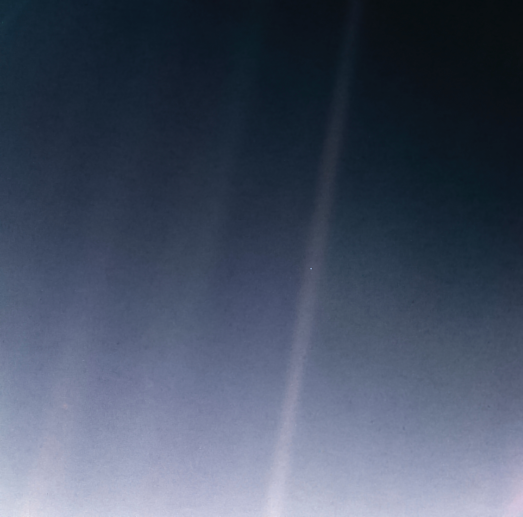
\includegraphics[align=t,width=\textwidth]{palebluedot2.png}}
\huge\sffamily%
\bfseries\color{white}}
\posttitle{\par\end{center}\bigskip}

\makeatletter\newcommand*{\atf}{
\includegraphics[totalheight=\heightof{@}]{pglpm_latex/atblack.png}}\makeatother
% \providecommand{\affiliation}[1]{\textsl{\textsf{\footnotesize #1}}}
\providecommand{\epost}[1]{\texttt{\footnotesize\textless#1\textgreater}}
\providecommand{\email}[2]{\href{mailto:#1ZZ@#2 ((remove ZZ))}{#1\protect\atf#2}}
%\providecommand{\email}[2]{\href{mailto:#1@#2}{#1@#2}}

\preauthor{\begin{center}\color{white}
\Large\sffamily%
}
\postauthor{\par\end{center}}
\predate{\DTMsetdatestyle{mydate}\begin{center}\footnotesize\color{white}}
\postdate{\par\end{center}}

\setfloatadjustment{figure}{\footnotesize}
\captiondelim{\quad}
\captionnamefont{\footnotesize\sffamily%
}
\captiontitlefont{\footnotesize}
%\firmlists*
\midsloppy
% handling orphan/widow lines, memman.pdf
% \clubpenalty=10000
% \widowpenalty=10000
% \raggedbottom
% Downes, memman.pdf
\clubpenalty=9996
\widowpenalty=9999
\brokenpenalty=4991
\predisplaypenalty=10000
\postdisplaypenalty=1549
\displaywidowpenalty=1602
\raggedbottom

\paragraphfootnotes
\setlength{\footmarkwidth}{2ex}
% \threecolumnfootnotes
%\setlength{\footmarksep}{0em}
\footmarkstyle{\textsuperscript{%\color{red}
\scriptsize\bfseries#1}~}
%\footmarkstyle{\textsuperscript{\color{red}\scriptsize\bfseries#1}~}
%\footmarkstyle{\textsuperscript{[#1]}~}

\selectlanguage{british}\frenchspacing
\usepackage{fontawesome5}

% \usepackage{wrapfig2}
% \newlength{\wfwidth}
% \setlength{\wfwidth}{0.4\linewidth}

\colorlet{mpcolor}{green}
%\newcommand*{\puzzle}{\maltese}
% \newcommand*{\puzzle}{{\fontencoding{U}\fontfamily{fontawesometwo}\selectfont\symbol{225}}}
% \newcommand*{\wrench}{{\fontencoding{U}\fontfamily{fontawesomethree}\selectfont\symbol{114}}}
% \newcommand*{\pencil}{{\fontencoding{U}\fontfamily{fontawesometwo}\selectfont\symbol{210}}}
\newcommand{\mynotew}[1]{{\footnotesize\color{midgrey}\faIcon{tools}\ #1}}
% \newcommand{\mynotep}[1]{{\footnotesize\color{notecolour}\pencil\ #1}}
% \newcommand{\mynotez}[1]{{\footnotesize\color{notecolour}\puzzle\ #1}}

%%%%%%%%%%%%%%%%%%%%%%%%%%%%%%%%%%%%%%%%%%%%%%%%%%%%%%%%%%%%%%%%%%%%%%%%%%%%
%%% Paper's details
%%%%%%%%%%%%%%%%%%%%%%%%%%%%%%%%%%%%%%%%%%%%%%%%%%%%%%%%%%%%%%%%%%%%%%%%%%%%
\title{\propertitle}
\author{%
\hspace*{\stretch{1}}%
%% uncomment if additional authors present
% \parbox{0.5\linewidth}%\makebox[0pt][c]%
% {\protect\centering ***\\%
% \footnotesize\epost{\email{***}{***}}}%
% \hspace*{\stretch{1}}%
\parbox{1\linewidth}%\makebox[0pt][c]%
{\protect\centering %%%***%%%Luca %P.G.L.  Porta Mana
 %\href{https://orcid.org/0000-0002-6070-0784}{\raisebox{0.5ex}{\protect
\includegraphics[height=1ex]{pglpm_latex/orcid_32x32.png}}}%
% \\\footnotesize
% Western Norway University of Applied Sciences%
% \quad\epost{\email{pgl}{portamana.org}}%
}%
%% uncomment if additional authors present
% \hspace*{\stretch{1}}%
% \parbox{0.5\linewidth}%\makebox[0pt][c]%
% {\protect\centering ***\\%
% \footnotesize\epost{\email{***}{***}}}%
\hspace*{\stretch{1}}%
}

%\date{Draft of \today\ (first drafted \firstdraft)}
\date{Version \version, updated \updated}

%%%%%%%%%%%%%%%%%%%%%%%%%%%%%%%%%%%%%%%%%%%%%%%%%%%%%%%%%%%%%%%%%%%%%%%%%%%%
%%% Macros @@@
%%%%%%%%%%%%%%%%%%%%%%%%%%%%%%%%%%%%%%%%%%%%%%%%%%%%%%%%%%%%%%%%%%%%%%%%%%%%

% Common ones - uncomment as needed
%\providecommand{\nequiv}{\not\equiv}
%\providecommand{\coloneqq}{\mathrel{\mathop:}=}
%\providecommand{\eqqcolon}{=\mathrel{\mathop:}}
%\providecommand{\varprod}{\prod}
\newcommand*{\de}{\uppartial}%partial diff
\newcommand*{\pu}{\piup}%constant pi
\newcommand*{\delt}{\deltaup}%Kronecker, Dirac
%\newcommand*{\eps}{\varepsilonup}%Levi-Civita, Heaviside
%\newcommand*{\riem}{\zetaup}%Riemann zeta
%\providecommand{\degree}{\textdegree}% degree
%\newcommand*{\celsius}{\textcelsius}% degree Celsius
%\newcommand*{\micro}{\textmu}% degree Celsius
% \newcommand*{\I}{\mathrm{i}}%imaginary unit
\newcommand*{\I}{\ensuremath{\mathrm{i}}}
% \newcommand*{\e}{\mathrm{e}}%Neper
\newcommand*{\e}{\ensuremath{\mathrm{e}}}
\newcommand*{\di}{\mathrm{d}}%differential
% \newcommand*{\dii}{\ensuremath{\mathrm{d}}}
% %% From TUGboat 18 (1997) 1 - leads to very strange spacing
% \makeatletter
% \providecommand*{\di}%
% {\@ifnextchar^{\DIfF}{\DIfF^{}}}
% \def\DIfF^#1{%
% \mathop{\mathrm{\mathstrut d}}%
% \nolimits^{#1}\gobblespace}
% \def\gobblespace{%
% \futurelet\diffarg\opspace}
% \def\opspace{%
% \let\DiffSpace\!%
% \ifx\diffarg(%
% \let\DiffSpace\relax
% \else
% \ifx\diffarg[%
% \let\DiffSpace\relax
% \else
% \ifx\diffarg\{%
% \let\DiffSpace\relax
% \fi\fi\fi\DiffSpace}
% \makeatother

% \newcommand*{\Di}{\mathrm{D}}%capital differential
%\newcommand*{\Li}{\mathrm{L}}%Lie derivative
%\newcommand*{\planckc}{\hslash}
%\newcommand*{\avogn}{N_{\textrm{A}}}
%\newcommand*{\NN}{\bm{\mathrm{N}}}
%\newcommand*{\ZZ}{\bm{\mathrm{Z}}}
%\newcommand*{\QQ}{\bm{\mathrm{Q}}}
\newcommand*{\RR}{\bm{\mathrm{R}}}
%\newcommand*{\CC}{\bm{\mathrm{C}}}
%\newcommand*{\nabl}{\bm{\nabla}}%nabla
%\DeclareMathOperator{\lb}{lb}%base 2 log
%\DeclareMathOperator{\tr}{tr}%trace
%\DeclareMathOperator{\card}{card}%cardinality
%% From TUGboat 18 (1997) 1
% \renewoperator{\Re}{\mathrm{Re}}{\nolimits}
% \renewoperator{\Im}{\mathrm{Im}}{\nolimits}
\DeclareMathOperator{\im}{Im}%im part
\DeclareMathOperator{\re}{Re}%re part
%\DeclareMathOperator{\sgn}{sgn}%signum
%\DeclareMathOperator{\ent}{ent}%integer less or equal to
%\DeclareMathOperator{\Ord}{O}%same order as
%\DeclareMathOperator{\ord}{o}%lower order than
% \newcommand*{\incr}{\triangle}%finite increment
\newcommand*{\incr}{\Delta}%finite increment
\newcommand*{\defd}{\coloneqq}
\newcommand*{\defs}{\eqqcolon}
%\newcommand*{\Land}{\bigwedge}
%\newcommand*{\Lor}{\bigvee}
%\newcommand*{\lland}{\DOTSB\;\land\;}
%\newcommand*{\llor}{\DOTSB\;\lor\;}
\newcommand*{\limplies}{\mathbin{\Rightarrow}}%implies
%\newcommand*{\suchthat}{\mid}%{\mathpunct{|}}%such that (eg in sets)
%\newcommand*{\with}{\colon}%with (list of indices)
%\newcommand*{\mul}{\times}%multiplication
%\newcommand*{\inn}{\cdot}%inner product
%\newcommand*{\dotv}{\mathord{\,\cdot\,}}%variable place
%\newcommand*{\comp}{\circ}%composition of functions
%\newcommand*{\con}{\mathbin{:}}%scal prod of tensors
%\newcommand*{\equi}{\sim}%equivalent to 
\renewcommand*{\asymp}{\simeq}%equivalent to 
%\newcommand*{\corr}{\mathrel{\hat{=}}}%corresponds to
%\providecommand{\varparallel}{\ensuremath{\mathbin{/\mkern-7mu/}}}%parallel (tentative symbol)
% \renewcommand*{\le}{\leqslant}%less or equal
% \renewcommand*{\ge}{\geqslant}%greater or equal
%\DeclarePairedDelimiter\clcl{[}{]}
%\DeclarePairedDelimiter\clop{[}{[}
%\DeclarePairedDelimiter\opcl{]}{]}
%\DeclarePairedDelimiter\opop{]}{[}%}
\DeclarePairedDelimiter\abs{\lvert}{\rvert}
%\DeclarePairedDelimiter\norm{\lVert}{\rVert}
\DeclarePairedDelimiter\set{\{}{\}} %}
%\DeclareMathOperator{\pr}{P}%probability
\newcommand*{\p}{\mathrm{p}}%probability
\renewcommand*{\P}{\mathrm{P}}%probability
%\newcommand*{\E}{\mathrm{E}}
%% The "\:" space is chosen to correctly separate inner binary and external rels
\renewcommand*{\|}[1][]{\nonscript\:#1\vert\nonscript\:\mathopen{}}
%\DeclarePairedDelimiterX{\cp}[2]{(}{)}{#1\nonscript\:\delimsize\vert\nonscript\:\mathopen{}#2}
%\DeclarePairedDelimiterX{\ct}[2]{[}{]}{#1\nonscript\;\delimsize\vert\nonscript\:\mathopen{}#2}
%\DeclarePairedDelimiterX{\cs}[2]{\{}{\}}{#1\nonscript\:\delimsize\vert\nonscript\:\mathopen{}#2}
%\newcommand*{\+}{\lor}
%\renewcommand{\*}{\land}
%% symbol = for equality statements within probabilities
%% from https://tex.stackexchange.com/a/484142/97039
% \newcommand*{\eq}{\mathrel{\!=\!}}
% \let\texteq\=
% \renewcommand*{\=}{\TextOrMath\texteq\eq}
% \newcommand*{\eq}[1][=]{\mathrel{\!#1\!}}
\newcommand*{\mo}[1][=]{\mathclose{}\mathord{\nonscript\mkern0.5mu#1\nonscript\mkern0.5mu}\mathopen{}}
%%
\newcommand*{\sect}{\S}% Sect.~
\newcommand*{\sects}{\S\S}% Sect.~
\newcommand*{\chap}{Chapter}%
\newcommand*{\chaps}{chs}%
\newcommand*{\bref}{ref.}%
\newcommand*{\brefs}{refs}%
%\newcommand*{\fn}{fn}%
\newcommand*{\eqn}{eq.}%
\newcommand*{\eqns}{eqs}%
\newcommand*{\fig}{fig.}%
\newcommand*{\figs}{figs}%
\newcommand*{\vs}{{vs}}
\newcommand*{\eg}{{e.g.}}
\newcommand*{\etc}{{etc.}}
\newcommand*{\ie}{{i.e.}}
%\newcommand*{\ca}{{c.}}
\newcommand*{\foll}{{ff.}}
%\newcommand*{\viz}{{viz}}
\newcommand*{\cf}{{cf.}}
%\newcommand*{\Cf}{{Cf.}}
%\newcommand*{\vd}{{v.}}
\newcommand*{\etal}{{et al.}}
%\newcommand*{\etsim}{{et sim.}}
%\newcommand*{\ibid}{{ibid.}}
%\newcommand*{\sic}{{sic}}
%\newcommand*{\id}{\mathte{I}}%id matrix
%\newcommand*{\nbd}{\nobreakdash}%
%\newcommand*{\bd}{\hspace{0pt}}%
%\def\hy{-\penalty0\hskip0pt\relax}
%\newcommand*{\labelbis}[1]{\tag*{(\ref{#1})$_\text{r}$}}
%\newcommand*{\mathbox}[2][.8]{\parbox[t]{#1\columnwidth}{#2}}
\newcommand*{\zerob}[1]{\makebox[0pt][c]{#1}}
\newcommand*{\tprod}{\mathop{\textstyle\prod}\nolimits}
\newcommand*{\tsum}{\mathop{\textstyle\sum}\nolimits}
%\newcommand*{\tint}{\begingroup\textstyle\int\endgroup\nolimits}
%\newcommand*{\tland}{\mathop{\textstyle\bigwedge}\nolimits}
%\newcommand*{\tlor}{\mathop{\textstyle\bigvee}\nolimits}
%\newcommand*{\sprod}{\mathop{\textstyle\prod}}
%\newcommand*{\ssum}{\mathop{\textstyle\sum}}
%\newcommand*{\sint}{\begingroup\textstyle\int\endgroup}
%\newcommand*{\sland}{\mathop{\textstyle\bigwedge}}
%\newcommand*{\slor}{\mathop{\textstyle\bigvee}}
%\newcommand*{\T}{^\transp}%transpose
%%\newcommand*{\QEM}%{\textnormal{$\Box$}}%{\ding{167}}
%\newcommand*{\qem}{\leavevmode\unskip\penalty9999 \hbox{}\nobreak\hfill
%\quad\hbox{\QEM}}
%% from TUGboat 18 (1997) 1:
%\providecommand*{\unit}[1]{\ensuremath{\mathrm{\,#1}}}

%%%%%%%%%%%%%%%%%%%%%%%%%%%%%%%%%%%%%%%%%%%%%%%%%%%%%%%%%%%%%%%%%%%%%%%%%%%%
%%% Custom macros for this file @@@
%%%%%%%%%%%%%%%%%%%%%%%%%%%%%%%%%%%%%%%%%%%%%%%%%%%%%%%%%%%%%%%%%%%%%%%%%%%%

\newcommand*{\widebar}[1]{{\mkern1.5mu\skew{2}\overline{\mkern-1.5mu#1\mkern-1.5mu}\mkern 1.5mu}}

% \newcommand{\explanation}[4][t]{%\setlength{\tabcolsep}{-1ex}
% %\smash{
% \begin{tabular}[#1]{c}#2\\[0.5\jot]\rule{1pt}{#3}\\#4\end{tabular}}%}
% \newcommand*{\ptext}[1]{\text{\small #1}}% for propositions
% \DeclareMathOperator*{\argsup}{arg\,sup}
\newcommand*{\furl}[2]{\href{#1}{#2}\pagenote{\url{#1}}}
\renewcommand*{\autoref}[2]{\sidepar{\vspace{-1ex}\footnotesize{\color{blue}\faIcon{hand-point-right}\enspace\sect\,\ref{#1} page\,\pageref{#1}}}\textcolor{blue}{#2}}

\newcommand*{\yr}{\bm{r}}
\newcommand*{\yv}{\bm{v}}
%
\newcommand*{\yN}{N}
\newcommand*{\yJ}{J}
\newcommand*{\yn}{n}
\newcommand*{\yj}{\bm{j}}
\newcommand*{\ya}{\varAlpha}
\newcommand*{\yrho}{\rho}
\newcommand*{\yM}{m}% m, and q_m for mass flow
\newcommand*{\yE}{E}
\newcommand*{\yU}{U}
\newcommand*{\yEk}{\yE_{\textrm{k}}}%T
\newcommand*{\yEp}{\yE_{\textrm{p}}}%V
\newcommand*{\yH}{\varPhi}% really used for heat-flow
\newcommand*{\yQ}{Q}% Q for time-integral
\newcommand*{\yW}{W}% A,W for time-integral
\newcommand*{\yR}{R}% for energy source
\newcommand*{\yg}{\bm{g}}% gravitational acceleration
\newcommand*{\yP}{\bm{P}}
\newcommand*{\yp}{\bm{p}}
\newcommand*{\yF}{\bm{F}}
\newcommand*{\yG}{\bm{G}}
\newcommand*{\yf}{\bm{f}}
\newcommand*{\yL}{\bm{L}}% L or H
%\newcommand*{\yl}{\bm{L}}
\newcommand*{\yT}{\bm{\tau}}% M or T or M_Q
\newcommand*{\ym}{\bm{M}}% M or T or M_Q
%\newcommand*{\yt}{\bm{\tau}}
\newcommand*{\yS}{S}
\newcommand*{\yB}{H}
\newcommand*{\yte}{T}%temperature
%
\newcommand*{\yto}{t_{0}}
\newcommand*{\yxo}{x_{0}}
\newcommand*{\yyo}{y_{0}}
\newcommand*{\yzo}{z_{0}}
\newcommand*{\Dt}{\incr t}
\newcommand*{\Dx}{\incr x}
\newcommand*{\Dy}{\incr y}
\newcommand*{\Dz}{\incr z}
\newcommand*{\Dth}{\tfrac{\incr t}{2}}
\newcommand*{\Dxh}{\tfrac{\incr x}{2}}
\newcommand*{\Dyh}{\tfrac{\incr y}{2}}
\newcommand*{\Dzh}{\tfrac{\incr z}{2}}
\newcommand*{\energym}{energy-mass}
\newcommand*{\masse}{mass-energy}
%%% Custom macros end @@@

% % https://latex.org/forum/viewtopic.php?t=878
% \newenvironment{widepar}%
% {\setlength{\rightskip}{-\marginparsep}\addtolength{\rightskip}{-\marginparwidth}}{\par}


\usepackage[retain-explicit-plus,quantity-product=\:]{siunitx}
%\sisetup{input-digits = 0123456789\piup}

% \usepackage{multimedia}
\usepackage[breakable,skins]{tcolorbox}

\newtcolorbox{myframe}{enhanced, no shadow, colback=white, colframe=midgrey, boxrule=1pt, breakable, after={\smallskip}}

\newtcolorbox[auto counter, number within=chapter]{exercise}[1][]{enhanced, no shadow, sharp corners, parbox=false, colback=yellow!5!white, colframe=yellow, boxrule=1pt, breakable,
  % fontupper=\small,
  fonttitle=\bfseries, after={\smallskip}, title=\hspace{-2ex}\faIcon{puzzle-piece}\enspace Exercise~\thetcbcounter,#1}

\newtcolorbox{warning}[1][]{enhanced, no shadow, parbox=false, colback=red!5!white, colframe=red, left=1ex, right=1ex, leftrule=0pt, rightrule=0pt, bottomrule=0.5pt, toprule=0pt, breakable,
% fontupper=\small, fonttitle=\bfseries\small,
fonttitle=\bfseries\footnotesize,
after={\smallskip}, title=\hspace{0ex}\faIcon{exclamation-circle}\enspace#1}

% \newtcolorbox{critique}[1][Critique]{enhanced, no shadow,parbox=false,center,
% width=0.9\linewidth, colback=blue!5!white, colframe=blue, boxrule=1pt, breakable, fontupper=\small, fonttitle=\bfseries\small, after={\smallskip}, title=\hspace{-2ex}\faIcon{microscope}\enspace#1}

\newtcolorbox{definition}[1]{enhanced, no shadow, colback=green!5!white, colframe=green, leftrule=0pt, rightrule=0pt, bottomrule=0.5pt, toprule=0pt, breakable, fonttitle=\bfseries\sffamily\footnotesize, after={\smallskip}, title=\hspace{-2ex}\faIcon{bookmark}\enspace#1}
%map-marker-alt

\newtcolorbox{extra}[1]{enhanced, no shadow, parbox=false,width=0.975\linewidth, center, colback=blue!5!white, colframe=blue, boxrule=0.5pt, breakable, fontupper=\small, fonttitle=\bfseries\small, after={\smallskip}, title=\hspace{-2ex}\faIcon{user-astronaut}\enspace#1}
% \newtcolorbox[auto counter, number within=chapter]{extra}[2][]{enhanced, no shadow, parbox=false,width=0.975\linewidth, flush right, colback=blue!5!white, colframe=blue, boxrule=0.5pt, breakable, fontupper=\small, fonttitle=\bfseries\small, after={\smallskip}, title=\hspace{-2ex}\faIcon{rocket}\enspace Curiosity~\thetcbcounter\enspace#2,#1}

%%%%%%%%%%%%%%%%%%%%%%%%%%%%%%%%%%%%%%%%%%%%%%%%%%%%%%%%%%%%%%%%%%%%%%%%%%%%
%%% Beginning of document
%%%%%%%%%%%%%%%%%%%%%%%%%%%%%%%%%%%%%%%%%%%%%%%%%%%%%%%%%%%%%%%%%%%%%%%%%%%%
% \firmlists

% \setlength{\wrapoverhang}{\parindent}
% \setlength{\intextsep}{1ex}% with wrapfigure
% % \setlength{\columnsep}{2em}% with wrapfigure

\makepagenote
\renewcommand*{\notedivision}{}
\renewcommand*{\pagenotesubhead}[3]{\clearpage\addsec{URLs for chapter #2}}
\renewcommand*{\pagenotesubheadstarred}[3]{\clearpage\addsec{URLs for chapter \textit{#3}}}
\renewcommand*{\notenuminnotes}[1]{\footnotesize #1.\space}
% \renewcommand{\prenotetext}{\begingroup\footnotesize}
% \renewcommand{\postnotetext}{\endgroup}
\sideparmargin{right}

% \newlength{\pagewidth}
% \setlength{\pagewidth}{\linewidth}
% \addtolength{\pagewidth}{\marginparsep}
% \addtolength{\pagewidth}{\marginparwidth}

%\usepackage{cancel}

\usepackage{eso-pic}
\newcommand\BackgroundPic{%
\put(0,0){%
\parbox[b][\paperheight]{\paperwidth}{%
\vfill
\centering
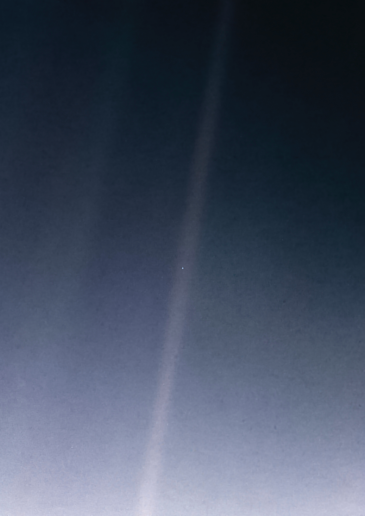
\includegraphics[width=\paperwidth,height=\paperheight,%
keepaspectratio]{palebluedotA4s.png}%
\vfill
}}}

%\usepackage[6-73,105-107]{pagesel}
\usepackage{tikz}
\usetikzlibrary{tikzmark}
\usetikzlibrary{arrows.meta}
% \usetikzlibrary{positioning}
% \newcommand{\tikzmark}[1]{\tikz[overlay,remember picture] \node (#1) {};}

\begin{document}
\AddToShipoutPicture*{\BackgroundPic}
\captiondelim{\quad}\captionnamefont{\footnotesize}\captiontitlefont{\footnotesize}
\selectlanguage{british}\frenchspacing

\begin{titlingpage}
\calccentering{\unitlength}
\begin{adjustwidth}{\unitlength}{-\unitlength}
  \centering
  % c6ddff % color of Earth in the Pale Blue Dot picture
  \color[HTML]{C6DDFF}
  \maketitle
\end{adjustwidth}
\end{titlingpage}
\killtitle

\calccentering{\unitlength}
\begin{adjustwidth*}{\unitlength}{-\unitlength}\thispagestyle{empty}
  \centering
  
\includegraphics[align=c,height=1em]{cc_by_sa.png} Licence

  \smallskip

%%%***%%%  Luca\enspace\href{https://orcid.org/0000-0002-6070-0784}{\raisebox{0.5ex}{\protect
\includegraphics[height=1ex]{pglpm_latex/orcid_32x32.png}}}{\footnotesize\url{https://orcid.org/0000-0002-6070-0784}}

\smallskip

Typeset with \LaTeX%\ using 12\,pt Palatino and Optima fonts

\bigskip

Cover image: the \enquote{Pale Blue Dot} image of the Earth taken by Voyager~1,
\\from right outside Pluto's orbit\\
\url{https://science.nasa.gov/resource/voyager-1s-pale-blue-dot/}
\end{adjustwidth*}
\setcounter{page}{0}


%%%%%%%%%%%%%%%%%%%%%%%%%%%%%%%%%%%%%%%%%%%%%%%%%%%%%%%%%%%%%%%%%%%%%%%%%%%%
%%% Abstract
%%%%%%%%%%%%%%%%%%%%%%%%%%%%%%%%%%%%%%%%%%%%%%%%%%%%%%%%%%%%%%%%%%%%%%%%%%%%
% \abstractrunin
% \abslabeldelim{}
% \renewcommand*{\abstractname}{}
% \setlength{\absleftindent}{0pt}
% \setlength{\absrightindent}{0pt}
% \setlength{\abstitleskip}{-\absparindent}
% \begin{abstract}\labelsep 0pt%
%   \noindent Lecture notes on introductory mechanics and thermodynamics (ING175)
% % \\\noindent\emph{\footnotesize Note: Dear Reader
% %     \amp\ Peer, this manuscript is being peer-reviewed by you. Thank you.}
% % \par%\\[\jot]
% % \noindent
% % {\footnotesize PACS: ***}\qquad%
% % {\footnotesize MSC: ***}%
% %\qquad{\footnotesize Keywords: ***}
% \end{abstract}
\selectlanguage{british}\frenchspacing

%%%%%%%%%%%%%%%%%%%%%%%%%%%%%%%%%%%%%%%%%%%%%%%%%%%%%%%%%%%%%%%%%%%%%%%%%%%%
%%% Epigraph
%%%%%%%%%%%%%%%%%%%%%%%%%%%%%%%%%%%%%%%%%%%%%%%%%%%%%%%%%%%%%%%%%%%%%%%%%%%%
% \asudedication{\small ***}
% \vspace{\bigskipamount}
\setlength{\epigraphwidth}{0.66\linewidth}
% %\epigraphposition{flushright}
% \epigraphtextposition{flushright}
% %\epigraphsourceposition{flushright}
% \epigraphfontsize{\footnotesize}
% \setlength{\epigraphrule}{0pt}
% %\setlength{\beforeepigraphskip}{0pt}
% %\setlength{\afterepigraphskip}{0pt}
% \epigraph{\emph{text}}{source}



%%%%%%%%%%%%%%%%%%%%%%%%%%%%%%%%%%%%%%%%%%%%%%%%%%%%%%%%%%%%%%%%%%%%%%%%%%%%
%%% BEGINNING OF MAIN TEXT
%%%%%%%%%%%%%%%%%%%%%%%%%%%%%%%%%%%%%%%%%%%%%%%%%%%%%%%%%%%%%%%%%%%%%%%%%%%%

\newpage
\setcounter{chapter}{-1}
\addchap{Introduction}
\label{sec:intro}

% \epigraphtextposition{flushright}
% %\epigraphsourceposition{flushright}
\epigraphfontsize{\footnotesize}
\setlength{\epigraphrule}{0pt}
% %\setlength{\beforeepigraphskip}{0pt}
% %\setlength{\afterepigraphskip}{0pt}
\epigraph{\emph{The loss implied in such an acquisition can be estimated only by those who have been compelled to unlearn a science that they might at length begin to learn it.}}{J. C. Maxwell \cites*{maxwell1878}}



Until some decades ago, the 18th-century physical notions typically taught in introductory Bachelor physics courses were enough to prepare an engineer for future specializations and jobs. Students who wanted to venture into modern theories, such as Relativity, were required to \textbf{re-learn} some of the most important physical notions -- \emph{Energy}, mass, time, entropy above all -- which in these theories are quite different from the 18th-century ones. But at that time the modern theories  still mostly had only theoretical, not practical, importance. So the re-learning efforts of the curious students could perhaps be justified.

\smallskip


% \marginpar{\footnotesize%
% {\color{mpcolor}\enquote{\emph{The achieved performances of atomic clocks and time
% transfer techniques imply that the definition of time scales
% and the clock comparison procedures must be considered
% within the framework of general relativity}}\sourceatright{\cites{petitetal2005}}}
% }
\marginpar{%
  {\color{mpcolor}\footnotesize%
    \enquote{\emph{Numerous relativistic issues and effects play roles in the global positioning system, on which millions of drivers, hikers, sailors, and pilots depend to find out where they are. The GPS system is, in effect, a realization of Einstein’s view of space and time. Indeed, the system cannot function properly without taking account of fundamental relativistic principles.}}\sourceatright{\cites{ashby2002}}}
}
%
That situation has changed today. Modern theories and modern physical notions are an essential part of many everyday technologies, such as nuclear reactors and the \furl{https://www.gps.gov}{Global Positioning System} (see the entertaining discussion in \cites[Project~A]{tayloretal2000}, and also \cites{petitetal2005,fliegeletal1996,ashby2002,muelleretal2008}). Modern theories and modern physical notions are required for the development of new technological possibilities, from \furl{https://www.ibm.com/topics/quantum-computing}{quantum computers} to solar sails, such as NASA's \furl{https://www.nasa.gov/mission/acs3/}{Advanced Composite Solar Sail System}. An engineering student (including communication, computer, and data engineering) may likely end up in a job that requires an understanding of modern physical notions. The diffusion of \furl{https://www.ibm.com/topics/large-language-models}{large language models} will moreover lead to a future demand for engineers who actually \textbf{understand} those physical notions, not little monkeys who have been trained to mechanically manipulate some equations while throwing some technobabble around. Automated large language models are faster, cheaper, and more precise in doing this kind of monkey activities. So why should one hire a human to do the same?

While moving from the older to the newer notions often requires re-learning efforts and conceptual re-orientations, the move in the opposite direction is less demanding. The modern physical notions are more encompassing than their 18th-century parents. Their understanding leads to an understanding of their older counterparts as approximate and special cases. Students, moreover, have often been hearing quite early  about the new notions from mass media; for instance about the equivalence of mass and energy, or about the discrepancy in time reckoning by different observers. Owing to this early exposure, students sometimes ask very intelligent and deep questions -- such as \enquote{\emph{should the mass of the body be included in its internal energy?}} -- when exposed to the old notions.



\medskip

It is therefore high time that introductory Bachelor physics courses be based on modern physical notions. Students should not be required to waste time and mental effort to learn something that they must unlearn and re-learn, only because of the inertia of academia and teachers.

Some teachers say \enquote{it would be too difficult for students to understand modern ideas, because they are too familiar with the old ones. This is why we need to teach the old and slightly incorrect ideas first, and correct them later}. I think that this kind of reasoning is scientifically unacceptable and leads to a vicious circle. Students are unfamiliar with new notions only because they were raised by a generation who was taught old ones. New notions become familiar only after a couple of generations learn them at an early stage. This is obvious if you consider that notions such as \enquote{energy}, \enquote{electromagnetic field}, \enquote{vector} are very familiar today, but were absolutely \emph{un}familiar a century or so ago. If we had always taught what's familiar, then we would still be teaching about the \emph{air, earth, water, fire} elements, and that the Sun revolves around the Earth. Arguments in favour of teaching old notions are for the most part just pretexts for laziness.

\medskip

The present lecture notes are an experiment and attempt to introduce classical mechanics and thermodynamics from modern physical notions and viewpoints. The core equations remain the same, but the students should have a broader conception of their meaning and of the symbols that appear in them.



% ** 6
% *** Importance of physics, necessity of maths: numbers (precision) and formulae (compact relations)
% *** Different languages (show examples) and points of view. What's chosen here
% *** Arena for physics (one point of view): space, time, "stuff"
%

\printpagenotes*
\clearpage
\chapter{Guide to the text}
\label{cha:guide}

\addsec{Maths prerequisites}
\label{sec:guide_maths}

\begin{itemize}
\item Working familiarity with algebra, its operations, and their properties, including square roots; knowledge of exponentials and logarithms is useful.
\item Working familiarity with solving equations and inequalities, linear and non-linear.
\item Working familiarity with the study of functions of one real variable.
\item Working familiarity with derivatives.
\item Understanding of what an integral is, even if you won't be required to solve integrals.
\item Working familiarity with vector calculus.
\item Some familiarity with functions of many variables.
\item Understanding of what partial derivatives are.
\end{itemize}


\addsec{Physics prerequisites}
\label{sec:guide_physics}

Just some vague reminiscences of secondary/high-school physics should be enough.

It can be beneficial if you are familiar with basic physics notions such as \emph{velocity}, \emph{mass}, \emph{force}, and similar ones; and if you vaguely remember about Newton's laws.

\addsec{Structure of this text}
\label{sec:guide_text}

\subsection{\faIcon{hand-point-right}\enspace Graphical devices}

The text includes the following graphical devices:
\begin{itemize}[para]
\item Important notions and definitions are also given in \textbf{boldface}.

\item\label{sec:self-reference}
  % \subsection{\faIcon{hand-point-right}\enspace References to previous topics}

The side margins often report clickable references to \autoref{sec:self-reference}{previous topics, emphasized in blue}.

\item Important-notion boxes:
  \begin{definition}{Some important notion or definition}
    This is a definition or explanation of Something.
  \end{definition}
\item Warnings and important points that require careful thinking:
  % \colorlet{shadecolor}{red}
  % \begin{shaded}
  %   Something you must be careful about.
  % \end{shaded}
  \begin{warning}[Careful!]
    Something you must be careful about.
  \end{warning}
\item Exercises:
  \begin{exercise}
    This isn't really an exercise
  \end{exercise}
% \item Possible objections you might be thinking about:
%   \begin{critique}[This isn't right!]
%     I have an objection here.
%   \end{critique}
\item Discussions and connections with more advanced physics:
  \begin{extra}{How things really are in quantum physics}
    Just for your curiosity. You don't need to remember any of this.
  \end{extra}
\end{itemize}

\subsection{\faIcon{hand-point-right}\enspace Side pictures and quotes}

\marginpar{\centering%
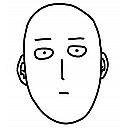
\includegraphics[align=c,width=0.5\linewidth]{saitama_image.png}%
\\[\jot]\footnotesize\flushleftright{\color{green}%
This is an image of Saitama, which actually has nothing to do with the text on the left.}
}%
Pictures, graphs, or quotes related to the material are displayed on the right.


\subsection{\faIcon{hand-point-right}\enspace Hyperlinks and bibliography}

Some words are hyperlinks, like this one about \furl{https://onepunchman.fandom.com}{One Punch Man}; you also recognize them because they have a little footnote number. The links' URLs are listed at the end of each chapter, just in case you're reading a printed copy and wonder what the link was.

\medskip

The text gives bibliographic references, like \enquote{\cites{einstein1905c}}, to scientific literature. The references are listed in the final Bibliography on page~\pageref{sec:biblio}.

These references are not part of the course and don't need to be \enquote{studied}. They are given for two reasons:
\begin{itemize}
\item For your own curiosity.

\item 
\marginpar{\raggedright\footnotesize%
{\color{mpcolor}\emph{%
\enquote{Believe nothing, O monks, merely because you have been told it, or because it is traditional, or because you yourselves have imagined it. Do not believe what your teacher tells you merely out of respect for the teacher.}}
\\[\jot](attributed to Gautama Buddha)}
}%
To back up what's written in the text.
In science you should not believe something just because you've read it somewhere. You should, as much as possible, go and check \emph{for yourself} \emph{how the logic behind the statement is proved} and \emph{what is the experimental evidence behind the statement}.
\end{itemize}

\subsection{\faIcon{hand-point-right}\enspace Notation and terminology}

Mathematical notation, as well as notation for physical dimensions, strictly follows the standards given by the \furl{https://www.nist.gov/pml/special-publication-811}{International System of Units (SI)}, listed for example in \cites{iso2009} and \cites{iso2019}.






\printpagenotes*
\clearpage
\chapter{Physics?}
\label{cha:physics_general}

% \section{Magic}
% \label{sec:magic}

If you think about it, many things we ordinarily do every day are some sort of magic. Think of how you can instantaneously see and speak with a person living on another continent, in real time, using just a small widget in the palm of your hand. Think of how you can instantaneously see where you are on the Earth, using the same widget. Think of how fast you can go to another country, by flying in a huge metal thing. Think of how you can command and interact with a purely fictitious animated world when you play on your computer. The list can go on forever. Other things are luckily less ordinary, but still inspire a lot of awe: think of the devastating power unleashed by something roughly as small as a tennis ball, in an atomic bomb.

We can do these astonishing things thanks to our understanding of how the world works. That's Physics.

\medskip

Many things can be said and have been said about science and physics. Rather than repeating what's been already written in many excellent books, I invite you to take a break here and go read their introductions. Choose as you please; compare what they say; don't limit yourself to popular books.

\begin{center}
  \textellipsis
  \textellipsis
  \textellipsis
\end{center}


\section{Several possible formalisms or \enquote{languages}}
\label{sec:languages}

% Welcome back! The only thing about physics that I need to say here is that
Physics can be expressed and written from wildly different points of view, using wildly different principles. Let's call these \enquote{different physics languages}; a more technical name is \enquote{physics formalisms}. One may approach a physics phenomenon or problem in terms of \emph{Lagrangeans}, or \emph{Hamiltonians}, or \emph{fibre bundles}, or \emph{categories}, or \emph{action principles}, or many other formalisms.
\marginpar{\normalsize%
  \begin{gather*}
    \color{red}\delt\!\!\int\!\!L\,\di t = 0 \quad L=\frac12 m v^{2}
    \\
    \color{cyan}\bm{F}=\frac{\di}{\di t}m\bm{v} \quad \bm{F}=0
  \end{gather*}
%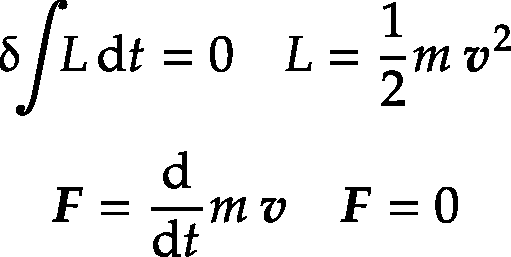
\includegraphics[align=t,width=\linewidth]{eg_languages.png}
{\footnotesize\color{mpcolor}%
Example of two different formalisms (\textcolor{red}{red}, \textcolor{cyan}{blue}) expressing the same physical phenomenon.\par%
}
}
These formalisms or languages are not completely separated; we know how to translate among them. In \enquote{doing} physics, one may jump among formalisms, because some ideas may be easier to express, or some results easier to find, in one formalism than another. No matter which physics formalism you choose, the results and the concrete applications are still the same. The choice is to a great extent subjective, based on your aesthetic tastes. You see that in \enquote{doing} physics you can express your personality and put your own artistic touch; this is why it's such a cool subject (and other scientific subjects are like this too).

In these notes I'm choosing one particular formalism: the one that for me is the most easily \emph{visualizable}; because I believe that visualization can be beneficial in learning new things. Or maybe I'm choosing it just because I like it best. I encourage you to explore how the physics you've learned is expressed in other physics formalisms; maybe you'll like another physics formalism better.

The formalism we'll be using might be called \enquote{field theory}. Roughly speaking it takes as starting point the ideas of space and time, or better spacetime, in which there are different kinds of \enquote{stuff}. It expresses the regularity and patterns that we observe in physical phenomena as \enquote{budgets} about the different kinds of stuff, and of relations between these kinds. Please don't take the description just given too literally; it's just meant to give you a very vague idea of the field-theoretical viewpoint.

\medskip

\marginpar{\footnotesize%
{\color{mpcolor}\enquote{\emph{this grand book, the universe, which stands continually open to our gaze. But the book cannot be understood unless one first learns to comprehend the language and read the
letters in which it is composed. It is written in the language of
mathematics}}\sourceatright{\cites{galilei1623}}}
}
It goes without saying that all these \enquote{physics languages} are to a great extent mathematical.

One reason is that numbers allow us to convey information in a concise and precise way. Imagine you have to tell someone, who doesn't know
Bergen, where in Bergen you are right now, to within 10\,m. You can do that with a description, \enquote{\textellipsis\ and there's a building called so-and-so which looks like so-and-so\textellipsis}, which would be lengthy and tricky. Or you can just give two numbers: latitude and longitude:
\begin{equation*}
  \num{60.36940},\ \num{5.3518} \ .
\end{equation*}
And in these two numbers all digits are important; for instance, the latitude is not \ensuremath{60.369\,4\bm{7}}.

But the most important reason is that mathematics allows us to describe and follow the patters and variety of physical phenomena in a greatly concise and precise way. And to develop their relationships in a rigorous way.
\marginpar{\footnotesize%
{\color{mpcolor}\enquote{\emph{There is nothing that can be said by mathematical symbols and relations which cannot also be said by words. The converse, however, is false. Much that can be and is said by words cannot successfully be put into equations, because it is nonsense.}}\sourceatright{\cites{truesdell1966}}}
}
All our present technology would have been impossible to discover, and would be impossible to realize, without the mathematical language of physics.

I invite you again to read what many good texts say about the relationship between physics and mathematics. No point repeating here what is said better elsewhere.

\section{Quantities: primitive and derived}
\label{sec:primitives}

One topic must be briefly discussed because it's important for understanding the notes that follow. It's the distinction between \emph{primitive} and \emph{derived} quantities.

I shall assume that you already know what a \textbf{physical quantity} is. Examples are: position, duration, velocity, pressure, energy, temperature.

A \textbf{derived quantity} is one that is defined in terms of other quantities. For example, velocity $\bm{v}$ (more precisely: average velocity) is defined as the ratio between a distance $\bm{d}$ (a vector) and a time duration $\bm{t}$:
\begin{equation*}
  \bm{v} \defd \frac{\bm{d}}{t}
\end{equation*}
where the symbol \enquote{$\defd$} means \enquote{is defined as} or \enquote{is defined by}. This means that in principle we could avoid using the word \enquote{velocity} and the symbol \enquote{$\bm{v}$} altogether, and instead always speak about distance and duration, using their symbols. It would lead to very long sentences and formulae and would be extremely inconvenient, but it could be done. The definition of a derived quantity often tells us how that quantity can be measured.

\marginpar{\centering%
\href{https://www.youtube.com/watch?v=nYg6jzotiAc&t=893s}{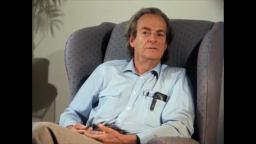
\includegraphics[align=t,width=\linewidth]{feynman_why2.png}}%
\\%
\flushleftright\footnotesize{\color{mpcolor}%
\emph{\enquote{you have to be in some framework that you allow something to be true. Otherwise you're perpetually asking \enquote*{why}}.}
(\furl{https://www.youtube.com/watch?v=nYg6jzotiAc&t=893s}{see video}).}%
}%
A derived quantity is defined in terms of other quantities, and these may in turn be derived quantities, that is, defined in terms of still other quantities, and so on. But at some point this chain of definitions must come to an end, otherwise we would go around in circles.

A \textbf{primitive quantity} is one that we do not define in terms of other quantities. Primitive quantities are the building blocks from which we define all others. That they are not defined in terms of others doesn't mean that we cannot try to explain them. But such explanations must be taken as informal and heuristic. Primitive quantities are often explained through metaphors and by appealing to intuition. You must always be wary of such explanations, because they may fail you spectacularly in some situations.

Often we have a choice about which quantities should be primitive and which should be derived. For instance, \emph{energy} can be defined, in a somewhat complicated way, in terms of quantities like \emph{work} and \emph{heat}, which would then need to be taken as primitive. Or we can take \emph{energy} as primitive, and define \emph{work} and \emph{heat} in terms of it. This second choice can be more convenient to develop a physical theory. It often happens that a quantity is very convenient for building a theory, if used as primitive; but difficult to understand intuitively. Vice versa,  a quantity can be very intuitive but lead to a complicated theory.
Among quantities which we'll take as primitive are:
\emph{time}, \emph{space} and \emph{length}, \emph{matter}, \emph{energy}, \emph{momentum},
% , \emph{rotational momentum},
\emph{entropy}, \emph{temperature}, and several others. All will be discussed soon.

 \section{Physical dimensions and units}
\label{sec:units}

\textbf{Measurement} is the process by which we determine the value of a physical quantity. Measurements can be extremely complex, and can extremely different even if they are about the same quantity. Consider the ways we can measure the mass of a football, compared to the ways we can measure the mass of the Sun.

To each quantity we associate a \textbf{physical dimension}. The term \enquote*{dimension} here has nothing to do with physical extension, as in \enquote{the dimensions of this box}; be careful not to confuse the two. Usually it's clear which one is meant from the context. Physical dimensions help us avoid making operations that don't make sense with some quantities. For example, it doesn't make sense to sum up the volume of a body of water with its temperature; and indeed the volume has dimension $\mathsf{length^{3}}$, whereas temperature has dimension $\mathsf{temperature}$, and quantities with different dimensions cannot be added up.

With each physical dimension we can associate a measurement \textbf{unit}, which expresses a basic standard for comparing the measurement results of similar quantities. For example, we could use the \emph{minute} or the \emph{second} as units to measure $\mathsf{time}$.

One can choose a basic set of physical dimensions from which to define all others, and for these a set of standard units. Here we shall follow the
\furl{https://www.nist.gov/pml/owm/metric-si/si-units}{International System of Units (SI)} (see also \furl{https://www.nist.gov/pml/special-publication-811}{NIST Special Publication 811}).

The topics of measurement and physical dimensions, which are studied in \emph{metrology} and in \emph{dimensional analysis}, could occupy an entire course by themselves. I shall assume that you already know their basics notions and that you read about the SI.

\smallskip

The measurement of some physical quantities consists in just one number with associated physical dimension; we shall call such quantity a \textbf{scalar}. The measurement of other physical quantities consists instead in a triplet of numbers with associated physical dimension; we shall call such quantity a \textbf{vector}.
\begin{warning}[What's scalar or vector depends on the theory]
  \emph{Scalar} and \emph{vector} have very specific and slightly different meanings in different theories, so don't take the definitions used here as universal. For example, in these notes and in Newtonian mechanics we call \emph{energy density} a scalar, but in general relativity it cannot be called a scalar.
\end{warning}

\section{Informal tips about units and maths}
\label{sec:units_maths}

\subsection{Importance of units}
\label{sec:importance_units}

Units are very important and must always be written for several reasons.

First, a number without units doesn't tell us anything. If I tell you \enquote{the place is at a distance 100 from here}, you have no idea how far the place is. \enquote{100} what? 100~metres? 100~kilometres? These are completely different distances.

Second, units give us useful information about mathematical objects and their physical relationships and measurement. If you see the expression \enquote{\qty{3}{m/s}}, then there's a strong possibility that that's a velocity. If you see the expression \enquote{\qty{5}{J/m^2}}, then you have a hint that it could be measured by measuring an energy and then dividing by an area.

Third, because of the previous reason, keeping track of units often allows us to quickly catch errors in solving a physical problem.

\subsection{Variables and units}
\label{sec:variables_units}

When a physical quantity is denoted by a symbol or variable, keep in mind that a unit is \enquote{contained} in the symbol, so to speak. For example if the variable $t$ denotes a time, then it includes some time unit, say seconds. This becomes apparent when we write the value of the symbol, for instance \enquote{$t=\qty{120}{s}$}. The unit is not predetermined, but it must correspond to the dimension of that quantity. We could for instance write \enquote{$t=\qty{2}{min}$} instead; the two expressions are completely equivalent.

This fact must be kept in mind when combining symbols. For example, if $d$ is a distance and $t$ is a time, then writing $v=d/t$ tells us that $v$ is a velocity, and it has appropriate units that come from $d$ and $t$, for instance \unit{m/s}.

Units otherwise behave just like \emph{literal constants} for all mathematical purposes, just like the letter \enquote*{$a$} in the expression \enquote*{$a\, x$}. This is why they can, for instance, be simplified:
\begin{equation*}
  \qty{3}{mol/s} \cdot \qty{5}{s} = 
  \num{3}\:\frac{\unit{mol}}{\not\unit{s}} \cdot \num{5}\:\not\unit{s} = \qty{15}{mol} \ .
\end{equation*}

\subsection{Mathematical functions and units}
\label{sec:functions_units}

Particular care must be taken with trigonometric and exponential functions, such as $\sin()$, $\cos()$, $\tan()$, $\exp()$, $\log()$; \textbf{these functions only admit a dimensionless argument} (which for the trigonometric ones corresponds to \emph{radians}). So there cannot be units like \enquote*{\unit{s}} or \enquote*{\unit{m}} within these functions: we must make sure that any units present within cancel out.

This makes sense, because we wouldn't know how to interpret the argument otherwise. Suppose you read \enquote{$\cos(\qty{60}{s})$} somewhere: how much is that? If we say \enquote{just discard the unit}, we would have
\begin{equation*}
  \cos(\qty{60}{s}) \stackrel{?}{=} \cos(60) \approx -0.95
\end{equation*}
but wait: $\qty{60}{s}\equiv\qty{1}{min}$, so we could equivalently write \enquote{$\cos(\qty{1}{min})$}. Then, according to the hypothetical rule \enquote{just discard the unit}, we would have
\begin{equation*}
  \cos(\qty{60}{s}) \equiv \cos(\qty{1}{min})\stackrel{?}{=} \cos(1) \approx +0.54
\end{equation*}
a completely different result!

For this reason an expression like \enquote*{$\cos(t)$}, with $t$ denoting time, doesn't make sense: there's a time unit in the argument of $\cos()$. If we want to express an oscillation with time, we must write instead something like
\begin{equation*}
  \cos\biggl(\frac{t}{T}\biggr)
\end{equation*}
where $T$ is the period of the oscillation, a symbol which also includes a time unit, which simplifies with the one in $t$. If the period of the oscillation is $T=\qty{1}{s}$ then we can also simply write
\begin{equation*}
  \cos(t/\unit{s})
\end{equation*}
This expression is now unambiguous: suppose that $t=\qty{60}{s}\equiv\qty{1}{min}$, then
\begin{equation*}
  \begin{aligned}
    \cos(t/\unit{s})
    &= \cos(\qty{60}{s}/\unit{s}) =\cos(60) \approx -0.95
    \\
    &= \cos(\qty{1}{min}/\unit{s}) =\cos(1\cdot 60\:\not\unit{s}/\not\unit{s}\bigr)
=\cos(60) \approx -0.95
  \end{aligned}
\end{equation*}

\smallskip

Also remember that \textbf{the results of trigonometric and exponential functions are dimensionless numbers}, so an expression like \enquote*{$3\,\cos(\dotso)$} denotes a pure number, with no units. If you want to express that the result is a length, the appropriate units must appear. We can for instance write
\begin{equation*}
  L\,\cos(\dotso)
\end{equation*}
where $L$ is a length, and therefore includes some kind of length unit such as \enquote*{\unit{m}}. If this length is, say, $L=\qty{2}{m}$ we can also simply write
\begin{equation*}
  2\,\cos(\dotso)\:\unit{m}
\end{equation*}

\subsection{Units and derivatives}
\label{sec:units_derivatives}

When we follow the rules above, all other mathematical operations automatically take care of everything. The derivative, for instance, is calculated in the usual way, treating any visible units as literal constants. Let's see a concrete example. This expression
\begin{equation*}
x(t) = 2\,\cos(t/\unit{s})\:\unit{m}
\end{equation*}
says that the position of some object oscillates with time, between the values \qty{-2}{m} and \qty{+2}{m}. When $t=\qty{0}{s}$, the position is $x=\qty{+2}{m}$. The position $x=\qty{-2}{m}$ is reached when the argument of $\cos()$ is $\pu$, that is
\begin{equation*}
  t/\unit{s} = \pu \quad\limplies\quad t\approx \qty{3.14}{s} \ .
\end{equation*}

The \autoref{sec:velocity}{velocity} of the object is given by the derivative of this expression with respect to $t$. Let's calculate it treating all unit symbols as literal constants:
\begin{equation*}
  \frac{\di x(t)}{\di t} = \frac{\di}{\di t}\Bigl(
  2\,\cos(t/\unit{s})\:\unit{m}
  \Bigr)
  =
  2\,\Bigl[
  \mathcolor{grey}{\underbracket{\color{black}-\sin(t/\unit{s})\cdot\frac{1}{\unit{s}}}_{\zerob{\color{grey}\footnotesize chain rule}}}
  \Bigr]\:\unit{m}
  =
 -2\,\sin(t/\unit{s})\:\unit{m/s}
\end{equation*}
and you see that the correct units for velocity have automatically appeared.

\clearpage

\section{What is \enquote{fundamental} physics?}
\label{sec:fundamental_physics}

But what's the \enquote{ultimate} goal of physics? What's \enquote{fundamental} physics? The answer to this question is again subjective -- also in this case physics lets you express your proclivities and personality. In the history of physics one can probably identify two main conceptions of \enquote{fundamental} physics.

For some physicists it is about finding the ultimate building blocks, so that one day we can say \enquote{\textellipsis and these are the constituents, and they obey these equations}. The history of physics seems to show that this goal is overturned every few generations. And yet every generation says \enquote{\emph{Now} we almost have the complete picture -- it's right behind the corner. It's true that previous generations thought they almost had it, and turned out to be wrong. But \emph{this time} is different, this time we have the real deal!}. The theoretical and particle physicist \furl{https://www.physics.lbl.gov/rememberinggeoffreychew/}{Geffrey Chew} depicted this situation as in \fig\,\ref{fig:chew1}. For this reason some physicists are a little sceptical about this goal; maybe it's a never-ending structure, with surprises at every deeper look.

So for other physicists fundamental physics is about finding some point of view or mathematical structure that is rich enough to make useful predictions, and yet flexible enough to accommodate any new patterns or objects that we might discover. In a manner of speaking, it is about finding \enquote{patterns of patterns} or \enquote{laws about physical laws}.

The two conceptions above are not mutually exclusive, and both are always pursued, even if time-changing fashions may emphasize the one or the other.

In these notes we take a point of view slightly closer to the second conception. This will also be reflected in the main division between physical laws that we'll draw in \chap\,\ref{cha:laws}.


\begin{figure}[p]
  \centering
  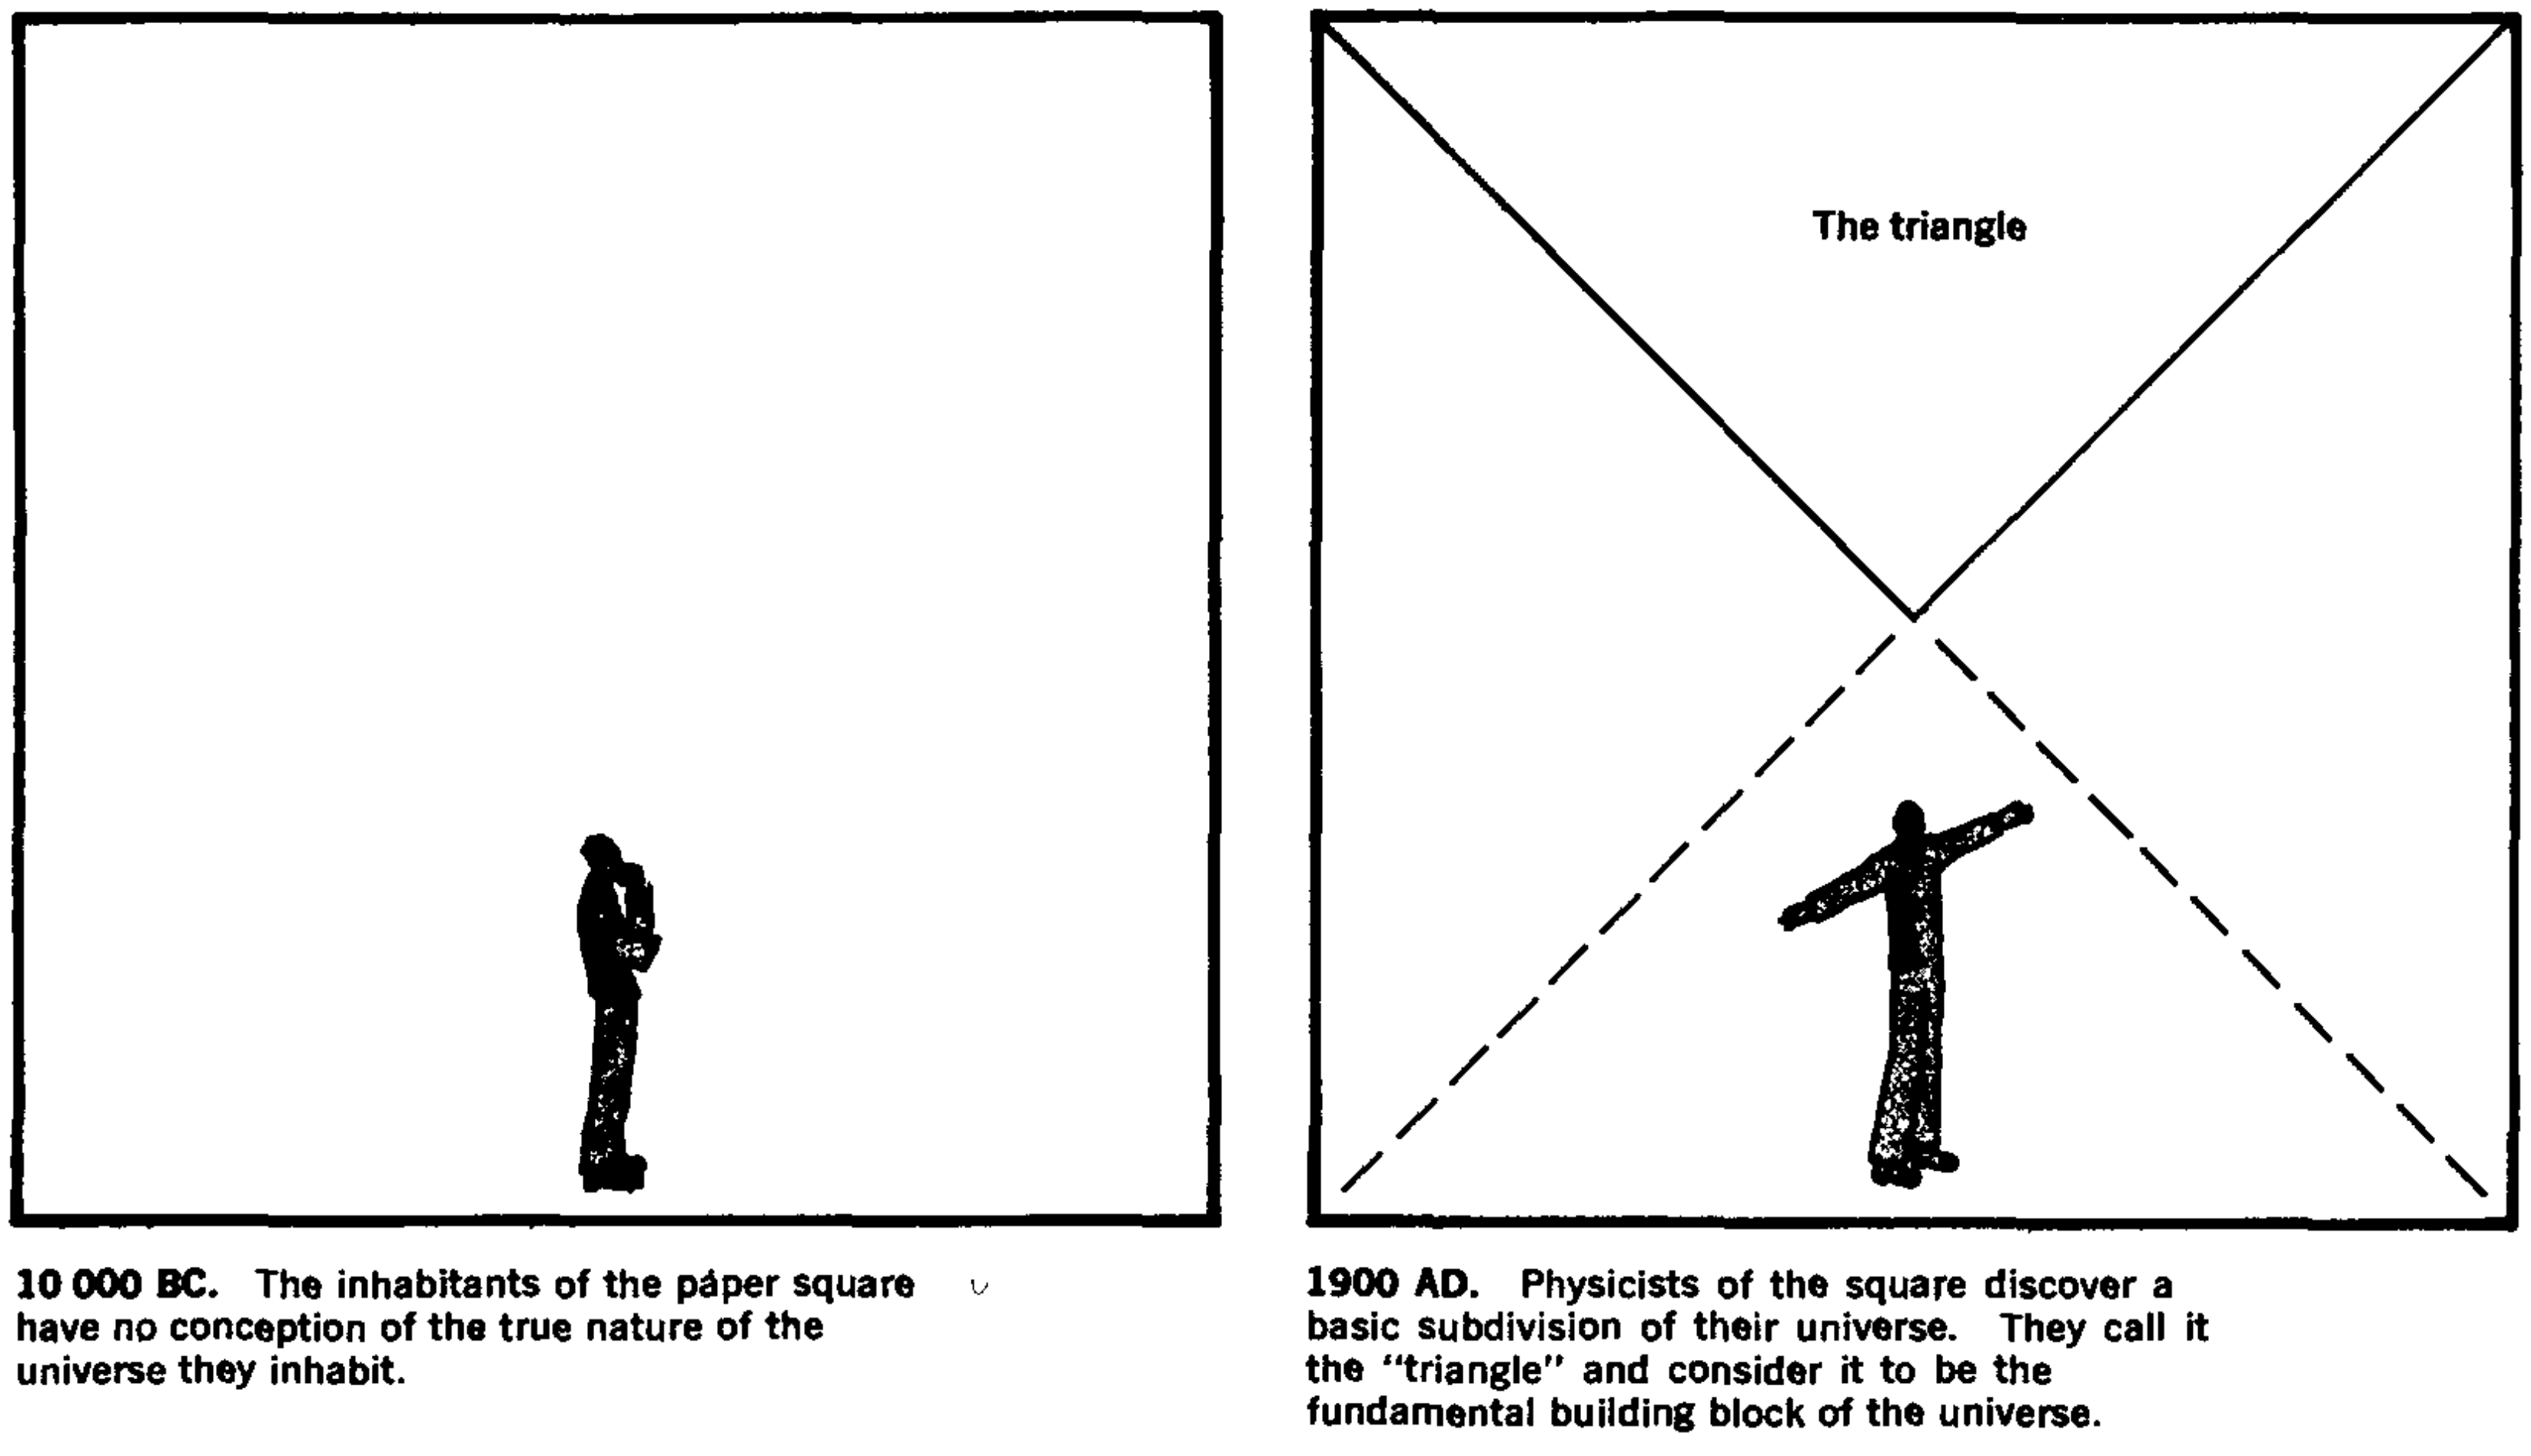
\includegraphics[width=1.2\textwidth]{chew1.png}
  \\[1em]  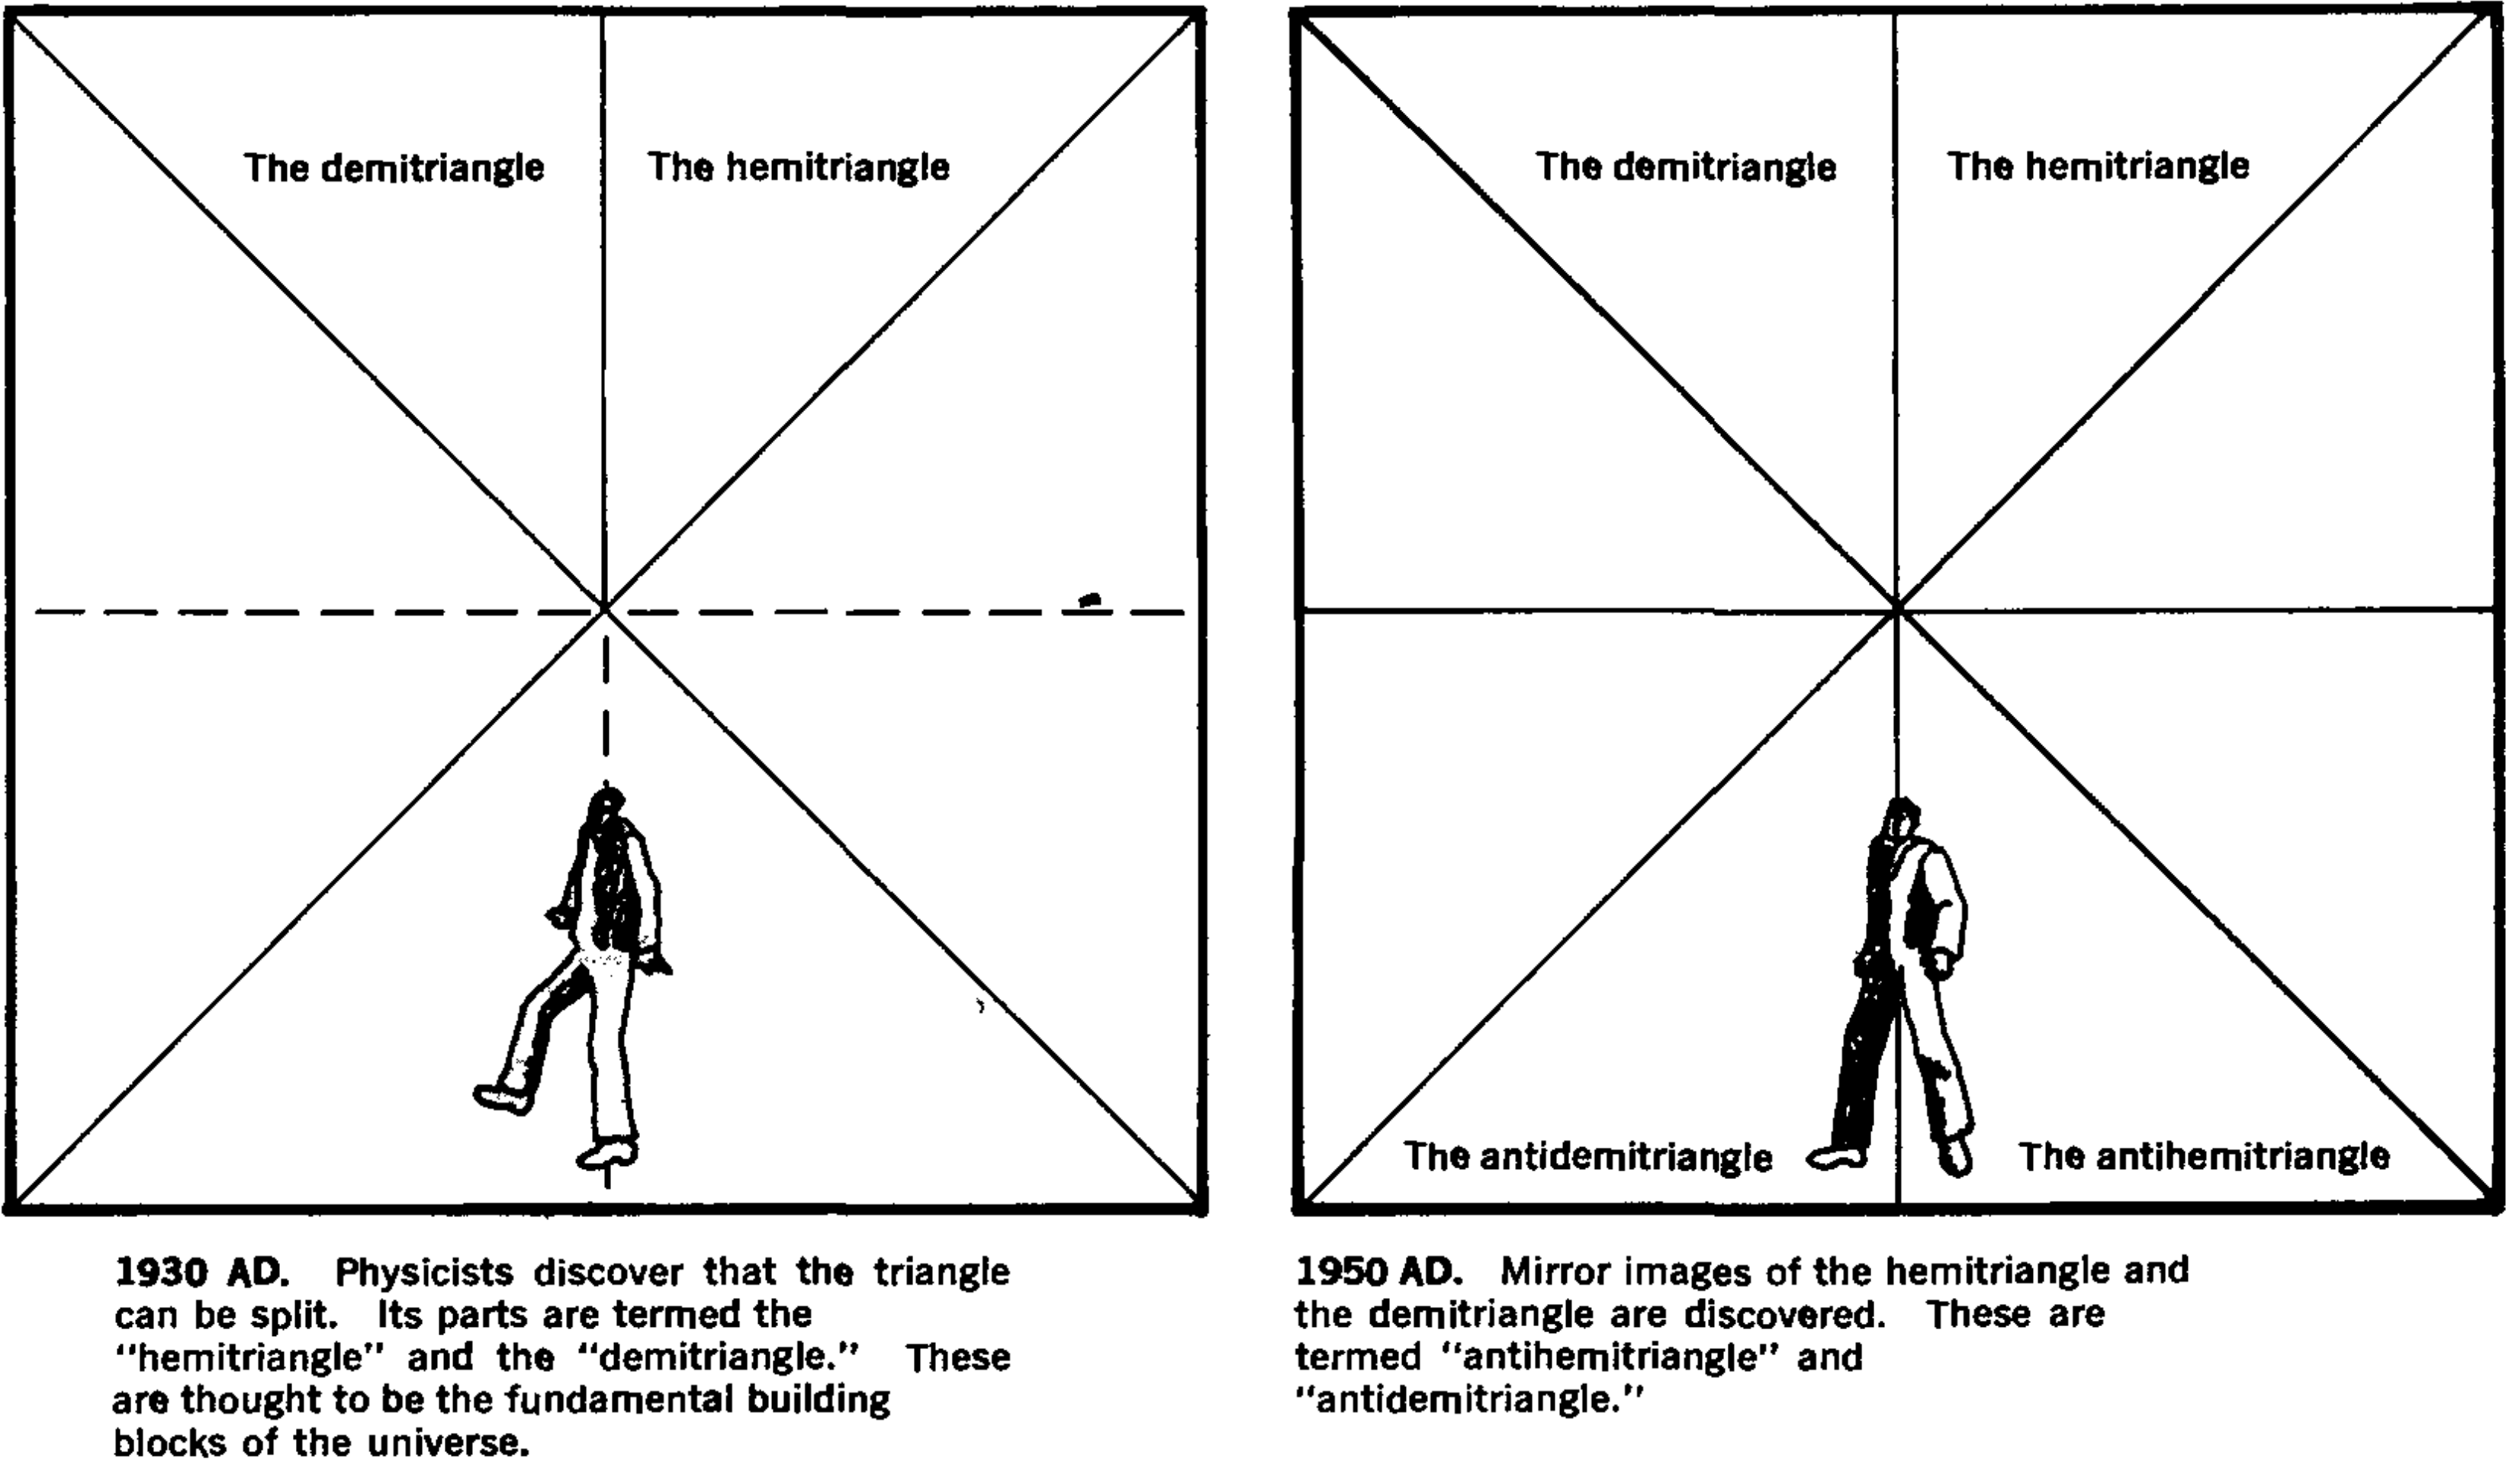
\includegraphics[width=1.2\textwidth]{chew2.png}
  \caption{(Continues on p.\,\pageref{fig:chew2}) \emph{The progress of \enquote{fundamental} physics}, from \cites{chew1970} as reproduced in \cites{truesdell1984_r1987}}
  \label{fig:chew1}
\end{figure}
\begin{figure}[p]
  \centering
  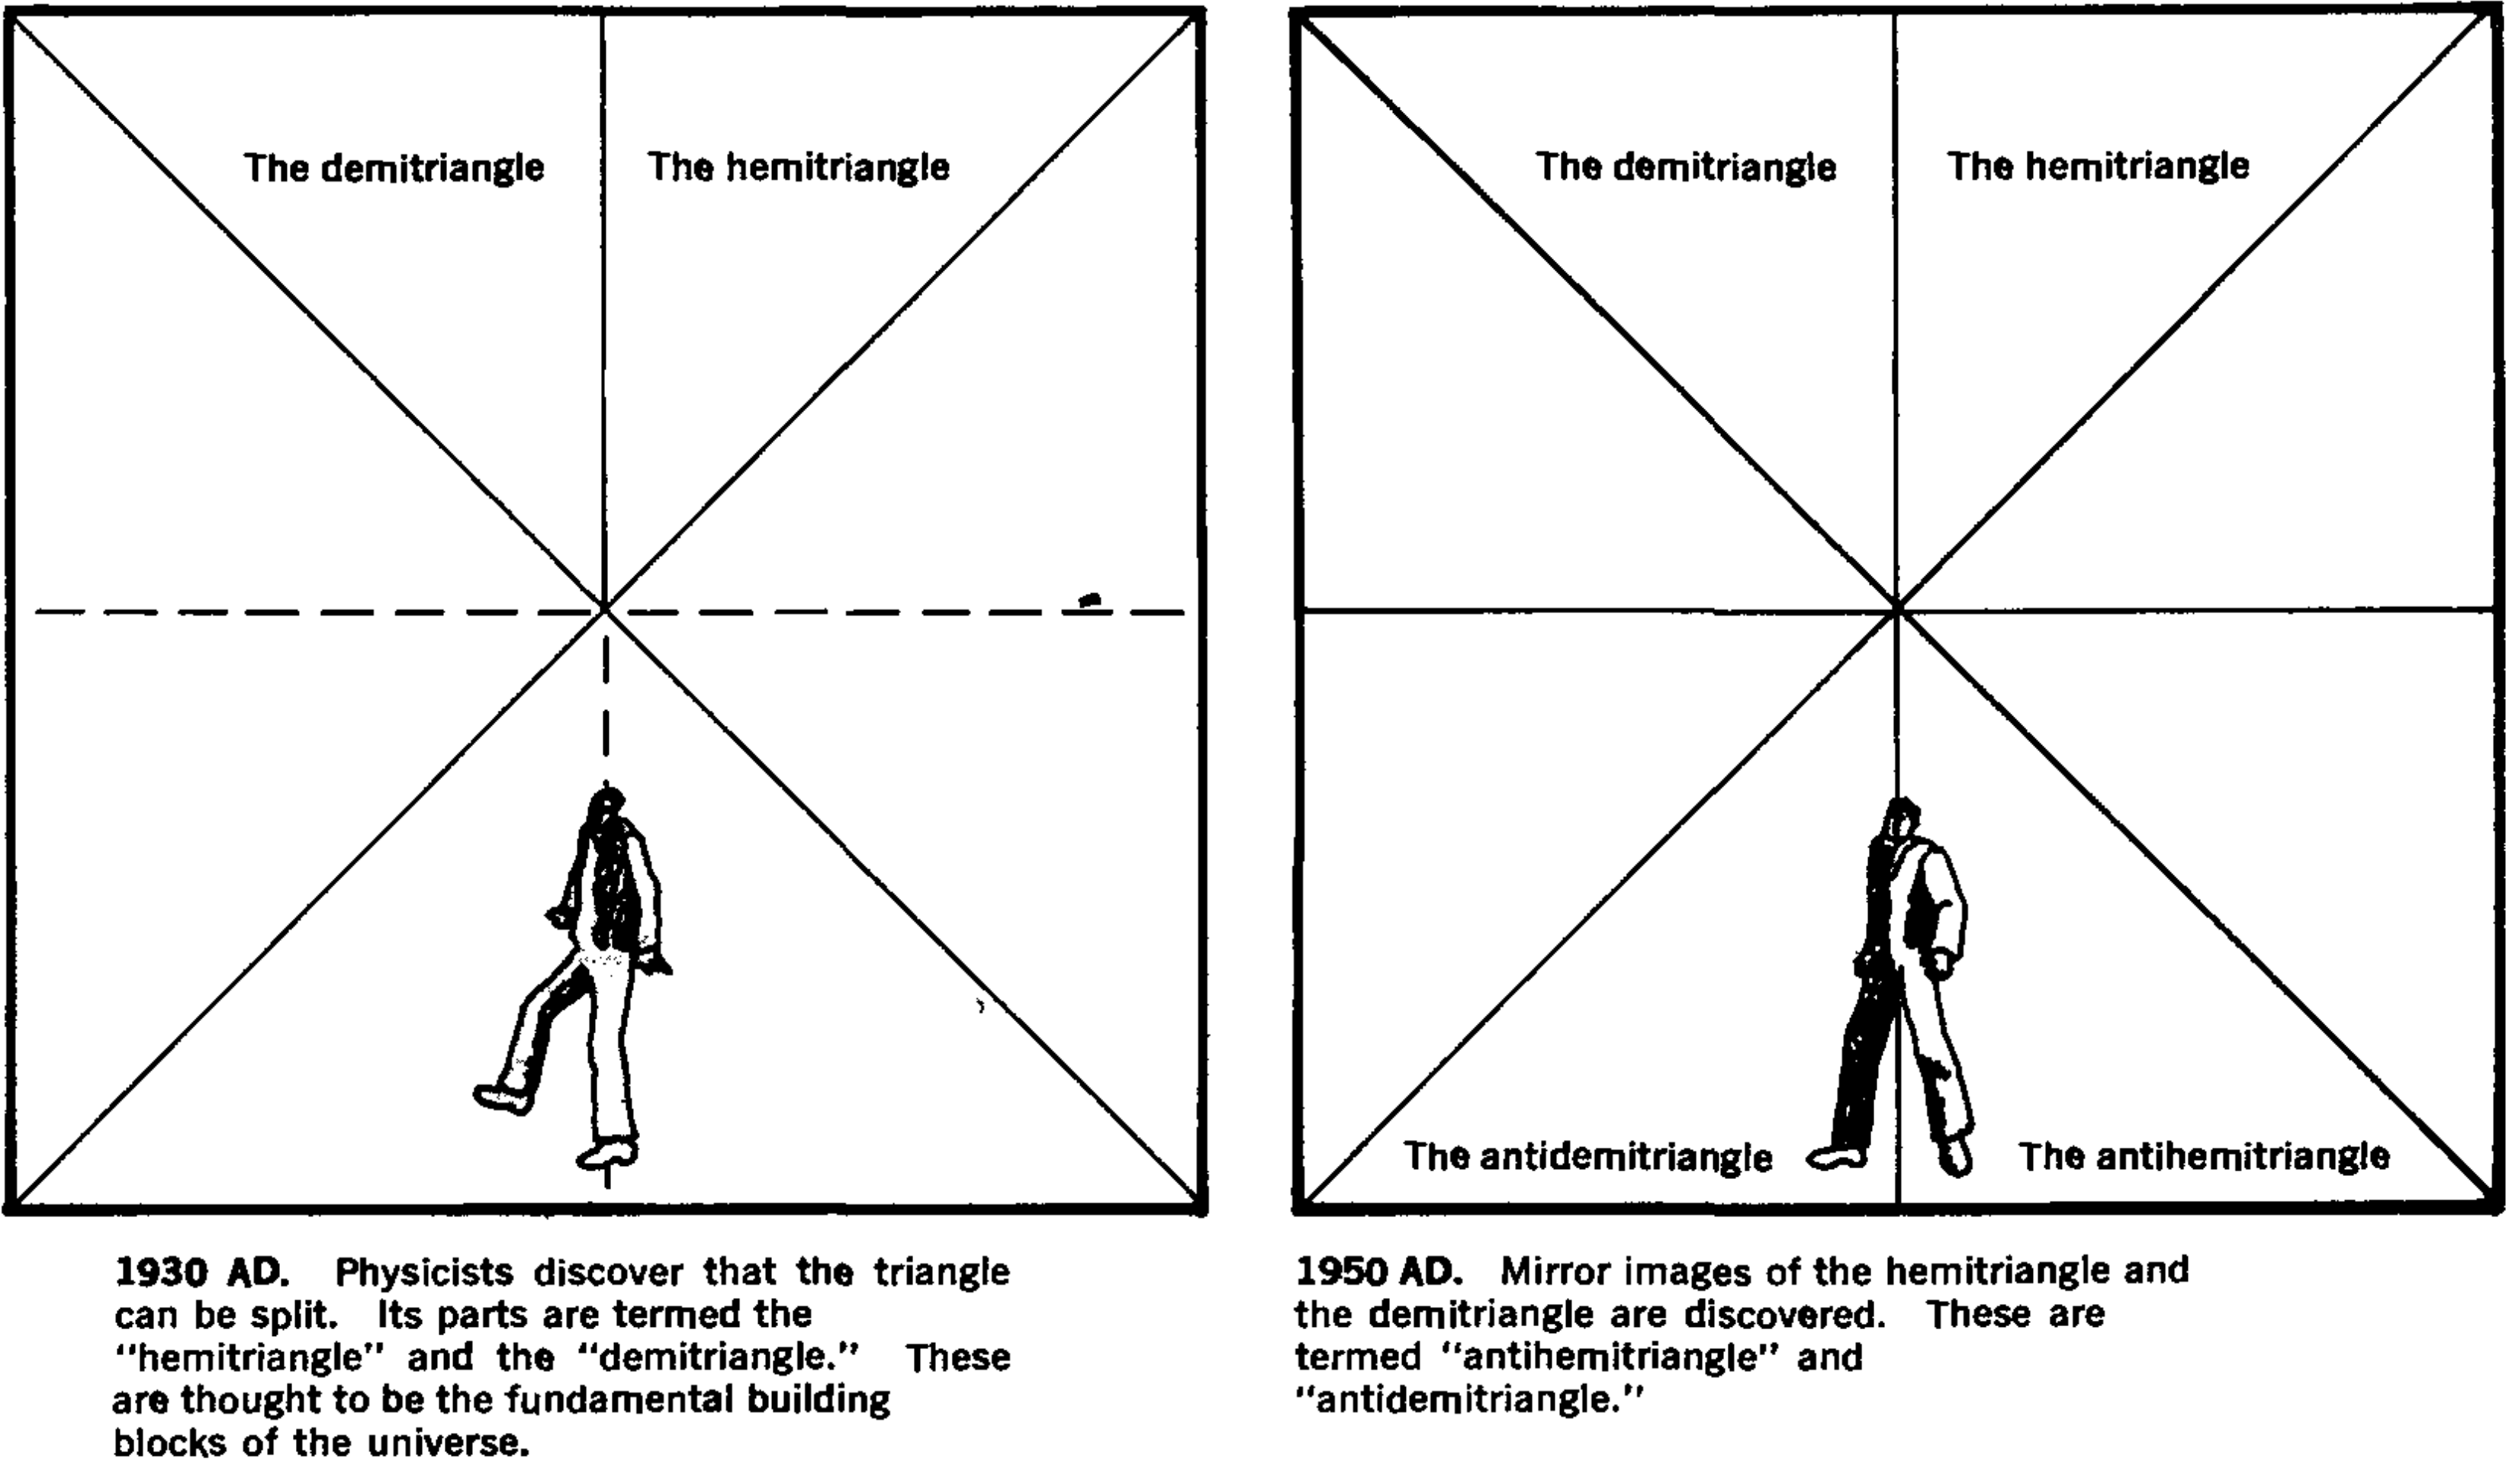
\includegraphics[width=1.2\linewidth]{chew3.png}
\\[1em]  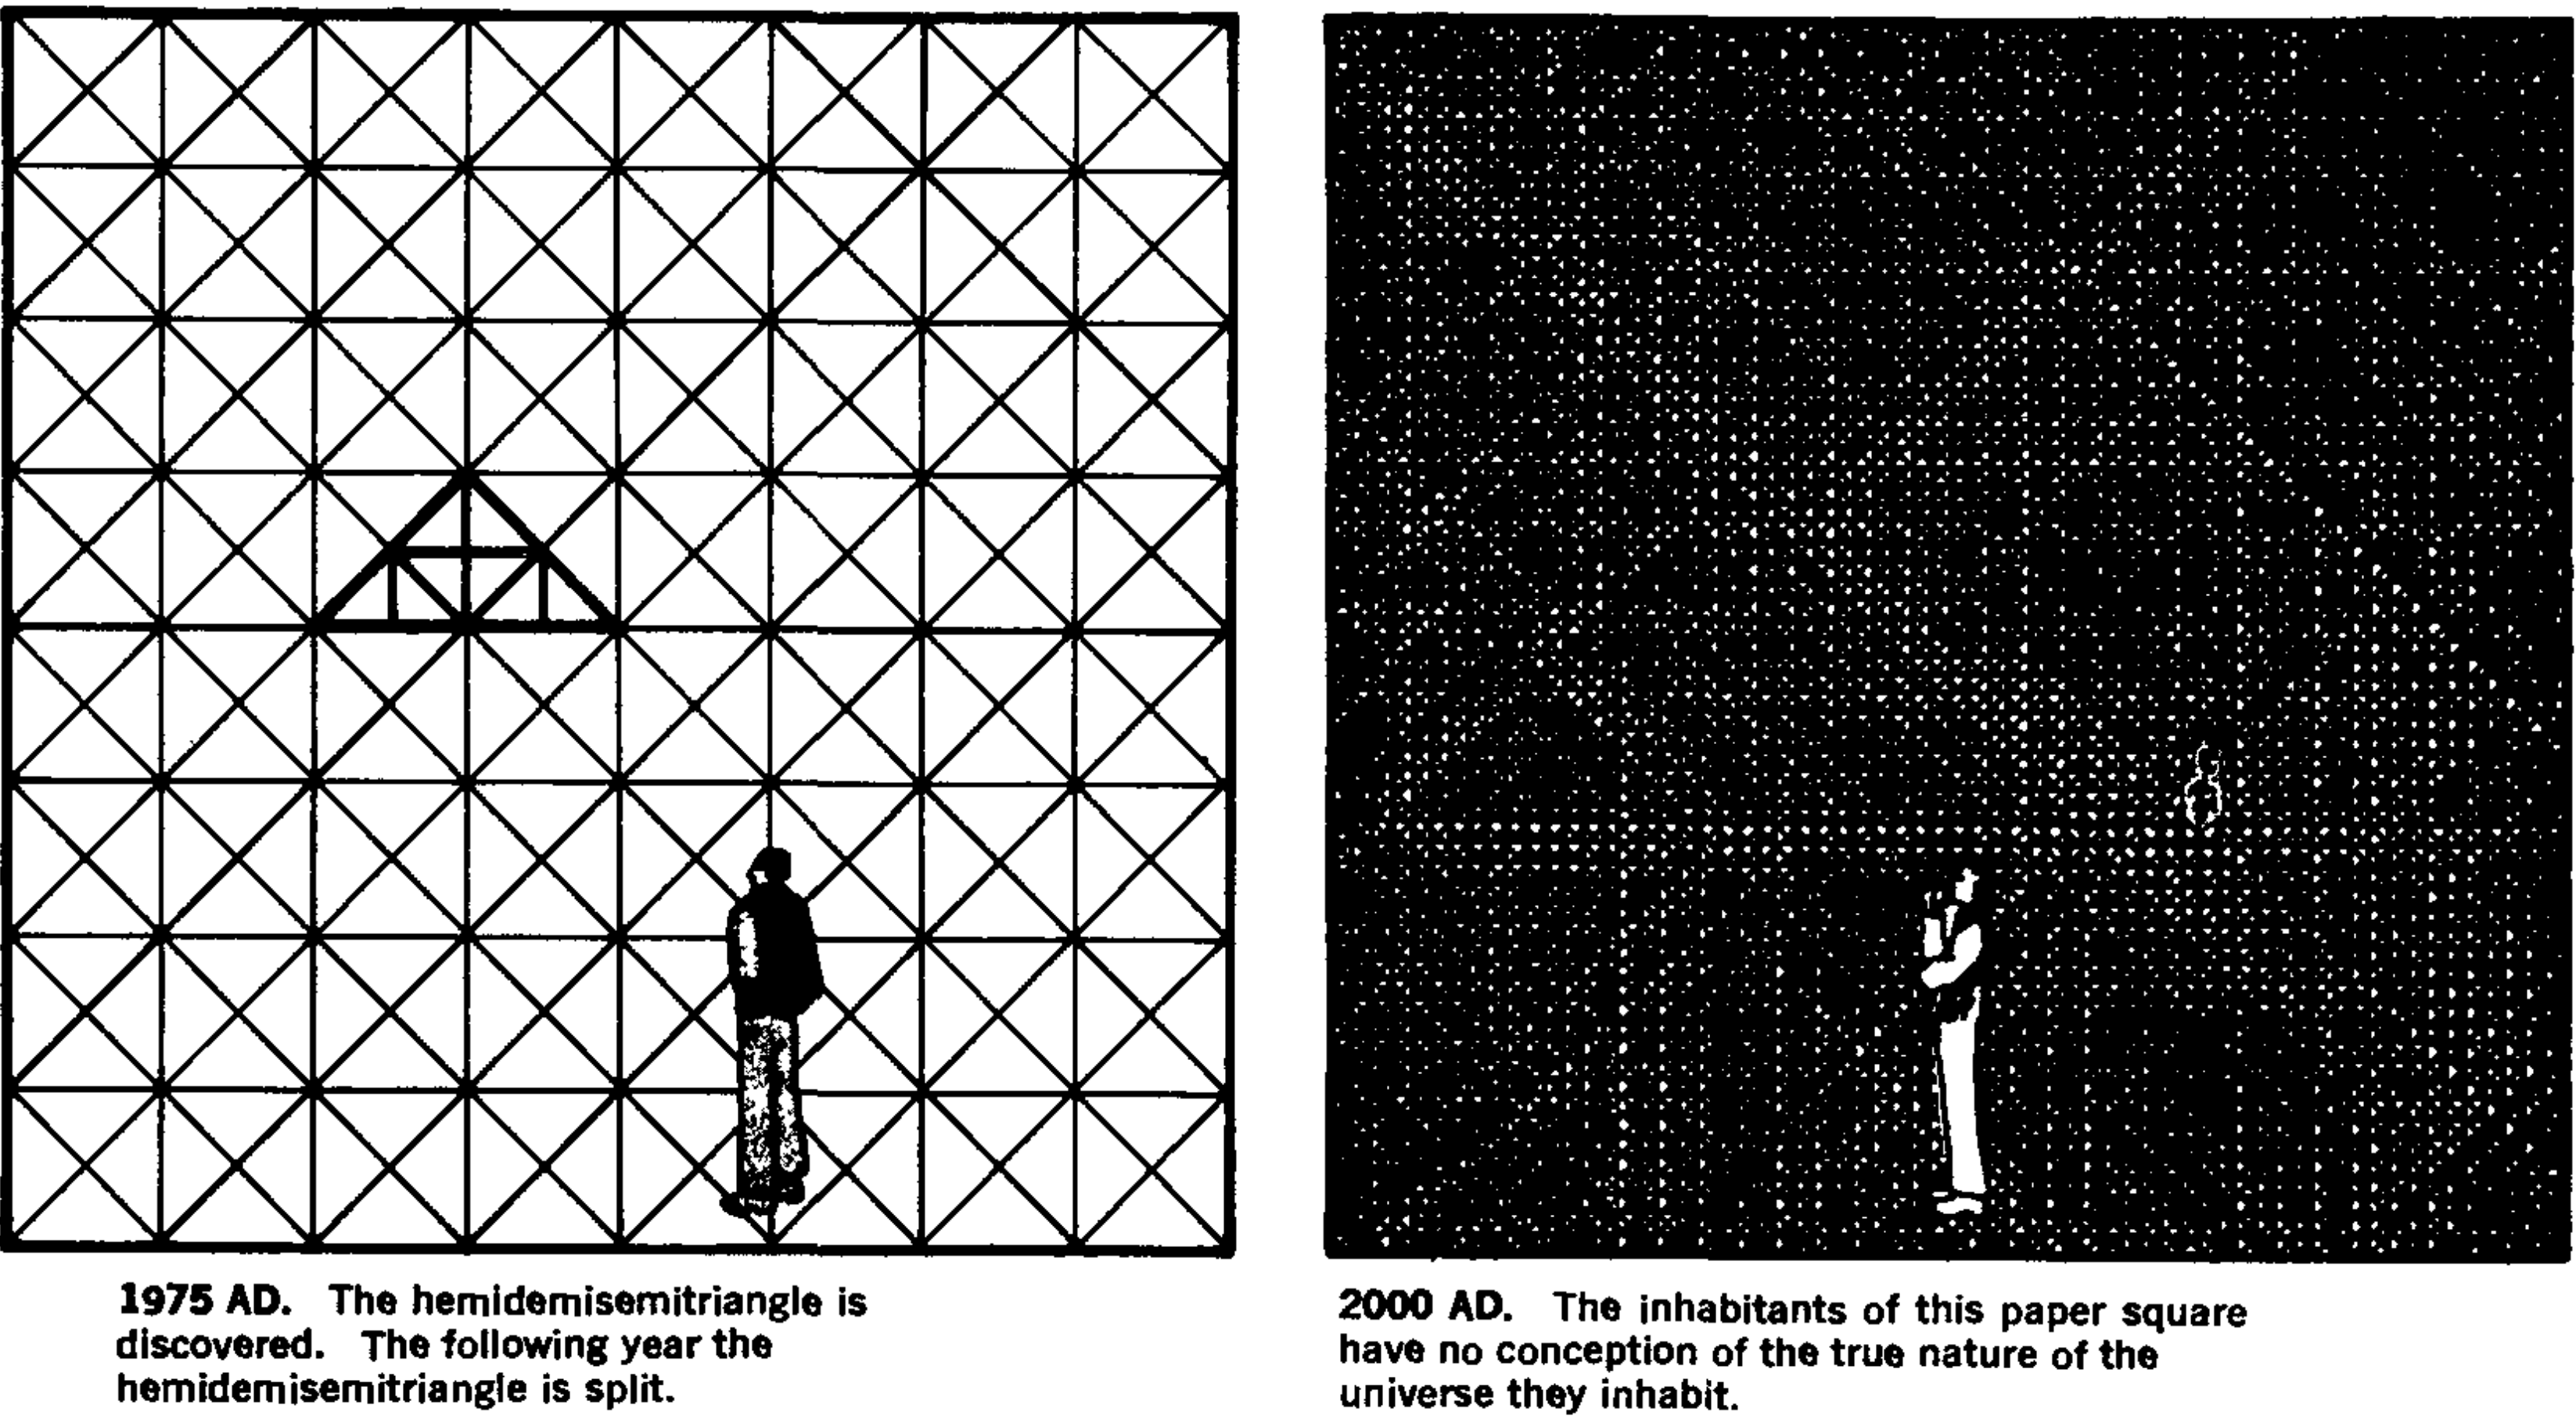
\includegraphics[width=1.2\linewidth]{chew4.png}
  % \caption{\emph{\enquote{The progress of \enquote*{fundamental} physics, conceived by Berkeley Chew, published in 1970 by his father, Professor Geoffrey F. Chew.}} Reproduced from  \cites{truesdell1984_r1987}}
  \label{fig:chew2}
\end{figure}


% ** 7
% *** Experimental characteristics of time measurement:
% **** time is not universal; for many purposes we must use a time _coordinate_ (maybe a simple spacetime diagram)
% **** GPS?
% **** luckily for many phenomena on Earth the difference is small
% *** Coordinate systems; vectors
% *** Experimental characteristic of quantities:
% **** quantities are "primitives"
% **** dependence on coordinate system

\printpagenotes*
\clearpage
\chapter{Building blocks: Time and space}
\label{cha:time_space}

\epigraph{\emph{If we want to describe the \emph{motion} of a material point, we give the values of its coordinates as a function of time. However, we should keep in mind that for such a mathematical description to have physical meaning, we first have to clarify what is to be understood here by \enquote{time}. We have to bear in mind that all our propositions involving time are always propositions about \emph{simultaneous events}. If, for example, I say that \enquote{the train arrives here at 7 o'clock}, that means, more or less, \enquote{the pointing of the small hand of my clock to~7 and the arrival of the train are simultaneous events}.}}{A. Einstein \cites*{einstein1905c}}

\section{Time}
\label{sec:time}

\emph{Time} is a primitive quantity. We understand the notion of time intuitively, even if it's difficult to explain (that's why it's taken as primitive). In 1905, with the theory of relativity, part of our everyday intuition about this notion was seriously shaken. For many years afterwards our old intuition could still be used in practice and in applications. But the new, correct intuition is becoming more and more important in everyday life and technologies. For example, GPS navigation -- which we use everyday from leisure activities such as hiking or sightseeing to more critical ones such as aeroplane landing -- critically depends on the correct notion and intuition of time.

Let's see how our traditional intuition goes astray with a concrete experiment. Here's Alice, Bob, and Charlie. They have extremely precise clocks built in exactly the same way. They stay very close to one another and synchronize their clocks. Still keeping close, they go around, maybe on an aeroplane or space ship, and all the time they check their clocks. They notice that their clocks stay perfectly synchronized all the time, no matter where they go and what they do.

At some point they separate, each one going around independently. One of them might stay in place, another might take a helicopter, and another might go for a trip on Mars and back.

Alice and Bob at some point meet again, and compare their clocks. They see that their clocks aren't synchronized anymore; the difference could be as small as microseconds, or as large as years. In fact, if this time discrepancy is large, they would notice that they themselves have aged differently; so time discrepancy doesn't affect the clocks only. Let's say for concreteness that Alice's clock is ahead of Bob's, or equivalently that Bob's is behind Alice's. Note the following aspects:

First, neither Alice or Bob can say \enquote{my clock was wrong}: neither has noticed anything strange about the \enquote{passage of time}.

Second, they might wonder what's the time on Charlie's clock. But Charlie is at some distance away. They could decide to contact Charlie via radio, say, and ask \enquote{what shows your clock right \emph{now}?}. But they would notice that there's a delay, even if extremely small, in the radio transmission; so it's unclear to what time would Charlie's answer apply. If we say \enquote{let's account for the radio-signal speed}, we see that there's a logical problem: speed is distance divided by time, and here we have a problem in exactly determining what's the \enquote{correct} time! So we would be reasoning in circles. Besides, even neglecting these difficulties, Charlie's answer could reveal a time that completely different from Alice's and from Bob's -- it could be years ahead or behind both of theirs!

Third, if they now stay together, they will see that their clocks remain exactly synchronized, besides the discrepancy they noticed when they met. This discrepancy doesn't increase or decrease. They may even retrace together Alice's and Bob's previous trips; their clocks still remain synchronized.

The experience just described will occur again any time two or more of them meet. There could be a hundred observers like Alice, Bob, Charlie, initially at the same place and synchronized. Whenever two or more of them meet after having been separated, they will notice discrepancies in their clocks. But their clocks will have exactly the same time lapses as long as they stay together. See the illustration in \fig\,\ref{fig:ABC_spacetime}

\begin{figure}[p]
  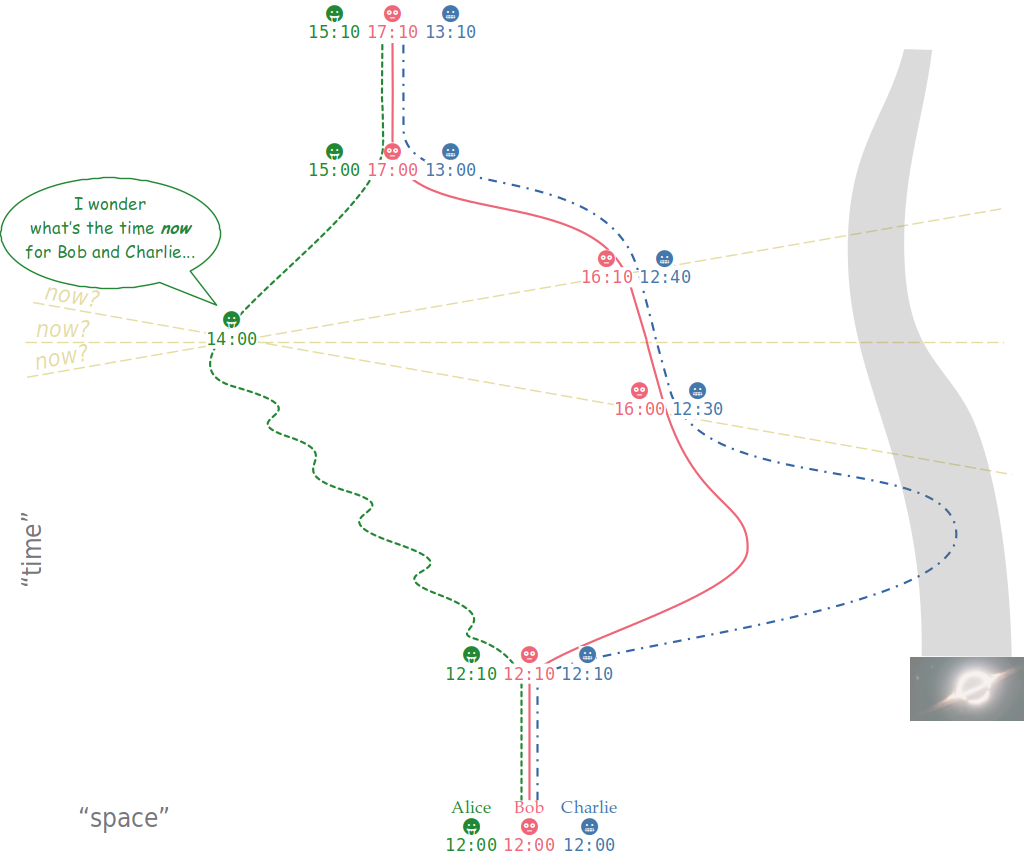
\includegraphics[width=\linewidth]{ABC_spacetime.png}
  \caption{Illustration of the experiences of Alice (\textcolor{green}{dashed \faIcon{grin-tongue}}), Bob (\textcolor{red}{solid \faIcon{flushed}}), Charlie (\textcolor{blue}{dot-dashed \faIcon{grimace}}) with time. The page represents a two-dimensional spacetime, and is followed from bottom to top.
\\\textbf{Bottom}: Alice, Bob, Charlie stay close and observe their clocks are perfectly synchronized from 12:00 to 12:10, then they separate.
\\\textbf{Right}: Charlie visits a region near a strong \masse\ source. Upon meeting again with Bob, the two notice their clocks differ: 16:00 for Bob, 12:30 for Charlie. Yet this clock difference stays the same while they travel together for \qty{10}{min}.
\\\textbf{Left}: Alice wanders around travelling at high speed with respect to the fixed stars. At some point she wonders what's the time \enquote{now} for Bob and Charlie. Obviously this question doesn't make sense, because
(1)~when Bob and Charlie are together their clocks differ -- impossible to say what's \enquote{the} time at their position; (2)~not clear which instant in Bob \amp\ Charlie's trajectory should be considered as \enquote{now} (\textcolor{yellow}{yellow dashed lines}).
\\\textbf{Top}: When all three meet again, their clocks have completely different readings; and they themselves have aged differently. But their clocks run again at the same rate as long as they stay close.}  \label{fig:ABC_spacetime}
\end{figure}
\clearpage

Consider for a moment an imaginary world in which these experiments had given a different kind of result. According to Newtonian mechanics, whenever two or more initially synchronized observers like Alice, Bob, Charlie had met, their clocks would have always shown exactly the same time. If one year, 23 days, 8 hours, 9 minutes, and \num{3.04539928324099266302} seconds have passed for you since you last met Alice, you'd see that exactly the same amount of time has passed for her when you two meet again. If you think about it, in this case it would have beeen somewhat natural to think \enquote{right now, the clocks of far-away Alice, Bob, Charlie must show the same time as mine} (even though you have no real experimental way of confirming that).

\marginpar{\footnotesize%
  {\color{mpcolor}\enquote{\emph{%
        In 1976, the International Astronomical Union introduced relativistic concepts of time and the transformations between various time scales and reference systems. \textelp{} Now \textelp{} it is necessary to base all astrometry, reference systems, ephemerides, and observational reduction procedures on consistent relativistic grounds. This means that relativity must be accepted in its entirety, and that concepts, as well as practical problems, must be approached from a relativistic point of view.}}\\{\cites{kovalevskyetal2004}}}
}
But that's an imaginary world. In our world is the more complicated situation described initially that holds. Only one conclusion can be drawn from these experimental results: \textbf{Time is not some sort of universal quantity. It is, so to speak, \enquote{local} to a person or clock, or to a group of persons or clocks that stick together.} This also means that \emph{it doesn't make sense} to ask questions like \enquote{what can be the time for far-away Charlie, right now?}. % \emph{Now} only applies to you, or to anything that is in your immediate vicinity.


The time measured by a specific observer is called the \textbf{proper time} of that observer. Luckily we know more about how the proper times of separated observers can differ when they meet again. It turns out -- according to our current understanding -- that the time differences depend, roughly speaking, on how fast the observers are moving with respect to one another and to matter around the universe, and on how much energy is contained in the regions they travel. The general theory of relativity gives us the equations determining any such proper-time differences.

The situation depicted in the experiments above is real. It can be measured, for example, comparing initially synchronized clocks that have been put in aeroplanes flying in different directions. Most importantly, it affects everyday relevant technologies such as the Global Positioning System. Formulae from general relativity appear in your phone's GPS software; see for instance \sect\,20.3.3.3.3 of the Interface Control Document \texttt{IS-GPS-200} at \url{https://www.gps.gov/technical/icwg/}. It must also be taken into account in the establishment and synchronization of time in our everyday equipments:
%\autocites[]{icwg1983_r2022}
\begin{quote}\footnotesize
  International Atomic Time (TAI) is based on more than 250 atomic clocks distributed worldwide that provide its stability, whereas a small number of primary frequency standards provide its accuracy. Universal Coordinated Time, which is the basis of all legal time scales, is derived from TAI. To allow the construction of TAI and the general dissemination of time, clocks separated by thousands of kilometres must be compared and synchronized. \textelp{} The achieved performances of atomic clocks and time transfer techniques imply that the definition of time scales and the clock comparison procedures must be considered within the framework of general relativity. \sourceatright{(\cites{petitetal2005})}
%\mbox{}\hfill (\cites{petitetal2005})
\end{quote}
% \begin{figure}[h!]\footnotesize\centering%
% 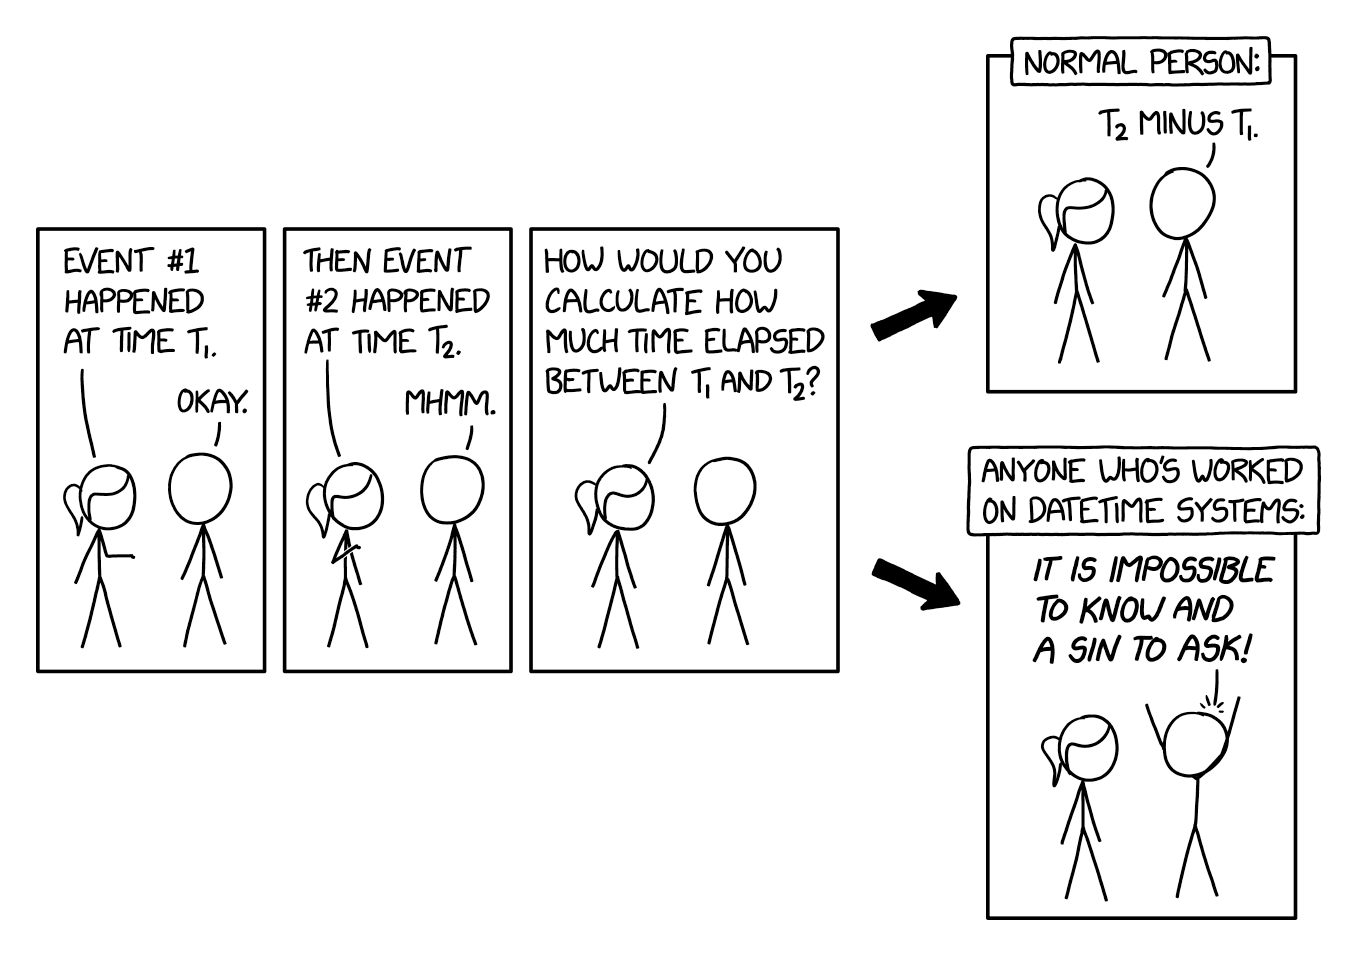
\includegraphics[align=t,width=0.75\linewidth]{datetime_2x.png}
% \\%
% \url{https://xkcd.com/2867}
% \end{figure}

\marginpar{\footnotesize%
{\color{mpcolor}\enquote{\emph{%
The plot for Cesium \textelp{} characterizes the best orbiting clocks in the GPS system. What this means is that after initializing a Cesium clock, and leaving it alone for a day, it should be correct to within \textelp{} 4~nanoseconds. Relativistic effects are huge compared to this.}}\sourceatright{\cites{ashby2003}}}
}
In most everyday situations for us, who live on or nearby Earth and move at speeds much smaller than $c$ with respect to one another, the discrepancies between our proper times are so small that cannot be
measured with ordinary clocks or with our internal clocks. Consider a
person walking \qty{10}{m} away from you and then immediately walking back
to you, at \qty{1}{m/s}. The time elapsed for you will be \qty{20}{s}, but for that person
will be \qty{19.999999999999999889}{s}, a difference of \qty{e-16}{s}, which is the error of an atomic clock. %%***add ref
If human beings still exist in some decades or centuries, with space travel they will probably have to deal more and more with proper-time discrepancies also in everyday life.

For the most part of the rest of these notes, we won't need to deal with differences in proper time. But I recommend that you keep present how time really works, and that these small time discrepancies exist and occur all the time along your \emph{worldline}.

\smallskip

Time has physical dimension of \textsf{time} and we shall for the most part measure it using the unit \emph{second}, symbol \enquote*{$\unit{s}$}.



\section{Space}
\label{sec:space}

Together with the notion of time, also the notion of space loses some of its traditional intuition. Several observers in motion with respect to one another will generally disagree on the dimensions of an approximately rigid object in their vicinity. For objects that are far away from an observer, the very notion of \enquote{distance} becomes tricky has different and non-equivalent definitions; one must be very careful on which definition is being used.

\smallskip

We shall not delve further into these peculiarities of time and space. Keep simply in mind that phenomena happen in \textbf{spacetime}, and that there's no way to attribute a universal time, nor a universal position in space, to a physical event. There is one absolute: whoever locally measures the speed of light, will find the value
\begin{equation}
  \label{eq:c}
  c\defd \qty{299792458}{m/s}
\end{equation}
This value is exact by definition, and serves as a way to define a local notion of space and distance.

\smallskip

Space has physical dimension of \textsf{length} and we shall for the most part measure it using the unit \emph{metre}, symbol \enquote*{$\unit{m}$}.


% In Bergen, a distance of 10\,m corresponds to a difference of 0.000\,1\,° in latitude or longitude


\section{Coordinate systems and events}
\label{sec:coords}

It is necessary to have a way for distinguishing physical events and phenomena and locating them in spacetime. This is achieved through a \textbf{coordinate system}.

A coordinate system assigns four numerical labels to every point in spacetime.
%
\marginpar{\centering%
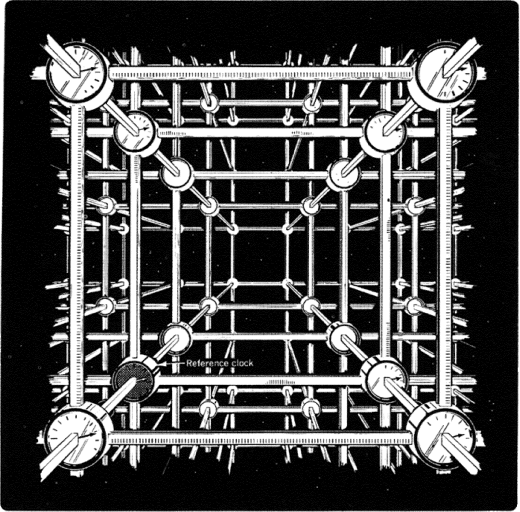
\includegraphics[align=t,width=\linewidth]{lattice_meters_clocks2.png}
\\[\jot]\footnotesize\flushleftright{\color{mpcolor}%
A lattice of clocks and meters, defining a spacetime coordinate system (from \cites{tayloretal2000})}%
}%
Often these labels have some kind of physical meaning -- such as the proper time elapsed for a specific clock, or the distance from some event as measured by a specific observer -- but they don't need to.

A coordinate system also solves the problems coming from proper-time and space discrepancies among different observers. We can assign to every physical event a \emph{coordinate time} and a \emph{coordinate spatial position}, which are the same for all observers, because decided by agreement. Coordinate time doesn't have a strict physical meaning, and will generally be different from the proper times registered by different observers. It can nevertheless be used for \enquote{doing physics}, and it is the time we shall most often use in our equations. A coordinate time commonly used for Earth-physics purposes is \furl{https://www.nist.gov/pml/time-and-frequency-division/time-realization/utcnist-time-scale-0/}{Universal Coordinated Time (UTC)}. The clock on your phone, and on devices that get synchronized via internet, shows UTC, not your proper time. An observer on Earth at \qty{0}{m} over sea level, and not moving, measures a proper time exactly equal to UTC (besides small variation coming from the movements of Solar System bodies). Observers at other altitudes or moving with respect to Earth's surface notice that their proper times are slightly different from UTC.

Up to now we have often used the word \enquote*{event}, informally taking its meaning for granted. Let's be more precise: we call \textbf{event} or \textbf{spacetime point} an extremely small region of space -- a point -- that only lasts for a very small lapse of time -- an instant. The name \enquote*{event} is used because typically we approximately identify such a point and instant by means of a physical phenomenon of limited spatial extension and short duration, such as the collision of two subatomic particles. The sudden burst of a very small soap bubble can be considered as an event in some circumstances; but something like \enquote{a tennis ball} cannot be considered as an event, mainly because a tennis ball exists for quite a long time, not just for a short instant. From a four-dimensional spacetime point of view,
%
\marginpar{\centering%
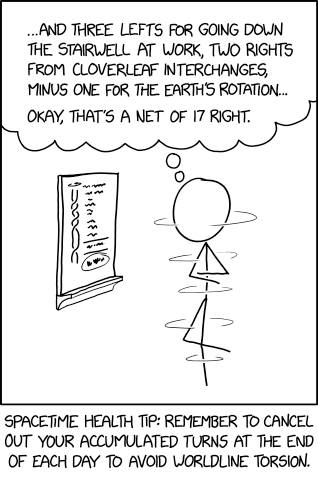
\includegraphics[align=t,width=\linewidth]{net_rotations.png}
\\\footnotesize{\color{mpcolor}%
\url{https://xkcd.com/2882}}%
}%
a tennis ball could be characterized as a line: a \textbf{worldline}.


\smallskip

We shall often denote the four coordinates of a coordinate system by the letters
\begin{equation*}
  (t, x, y, z)
\end{equation*}
where $t$ is a coordinate time, usually UTC, and $(x,y,r)$ determine a spatial position. The triplet of spatial coordinates is often denoted by the vector $\yr$:
\begin{equation*}
  \yr \defd (x,y,z)
  \qquad\text{or}\qquad
  \yr \defd [x,y,z]
  \qquad\text{or}\qquad
  \yr \defd
  \begin{bmatrix}
    x\\y\\z
  \end{bmatrix}
\end{equation*}
use round brackets \enquote*{$()$} or square brackets \enquote*{$[]$}, and horizontal or vertical notation as you prefer.

It is always important to specify how the coordinate system you're using is defined.
The definition of the spatial coordinates $(x,y,z)$ is typically different from problem to problem. We shall typically use coordinates that form $\frac{\pu}{2}\,\unit{rad} \equiv \ang{90}$ angles with one another; but their directions and their origin -- that is, where they have value $x=y=z=\qty{0}{m}$ -- always depend on the problem, so make sure you always specify them.

Whenever we speak of a \enquote{region of space} or of a \enquote{surface in space}, we mean a 3D or 2D region at some specific coordinate time $t$.

\smallskip

Some physical phenomena happen approximately along a line, in one dimension; or on a surface, in two dimensions. In these cases we can omit two or one of the spatial coordinates, assuming they have some constant, unimportant values; and we can simply write, for instance, $(t,x)$ or $(t,x,y)$ as our coordinates.

\begin{exercise}
  Consider a clock at rest on the Earth's surface, at a distance $\color{green}r_{\text{e}}$ from the Earth's centre; and a clock on a satellite, for instance a GPS satellite or the \furl{https://www.nasa.gov/international-space-station/}{International Space Station}, right above the first clock, at a distance $\color{red}r_{\text{s}}$ from the Earth's centre. An observer by the clock on Earth measuring a time lapse $\Dt_{\text{e}}$ will see the clock on the satellite has having run for a time lapse $\Dt_{\text{s}}$, and vice versa (note that this \enquote{vice versa} only holds in this specific situation!). The relation between two time lapses is approximately given by
\sidepar{\centering%
  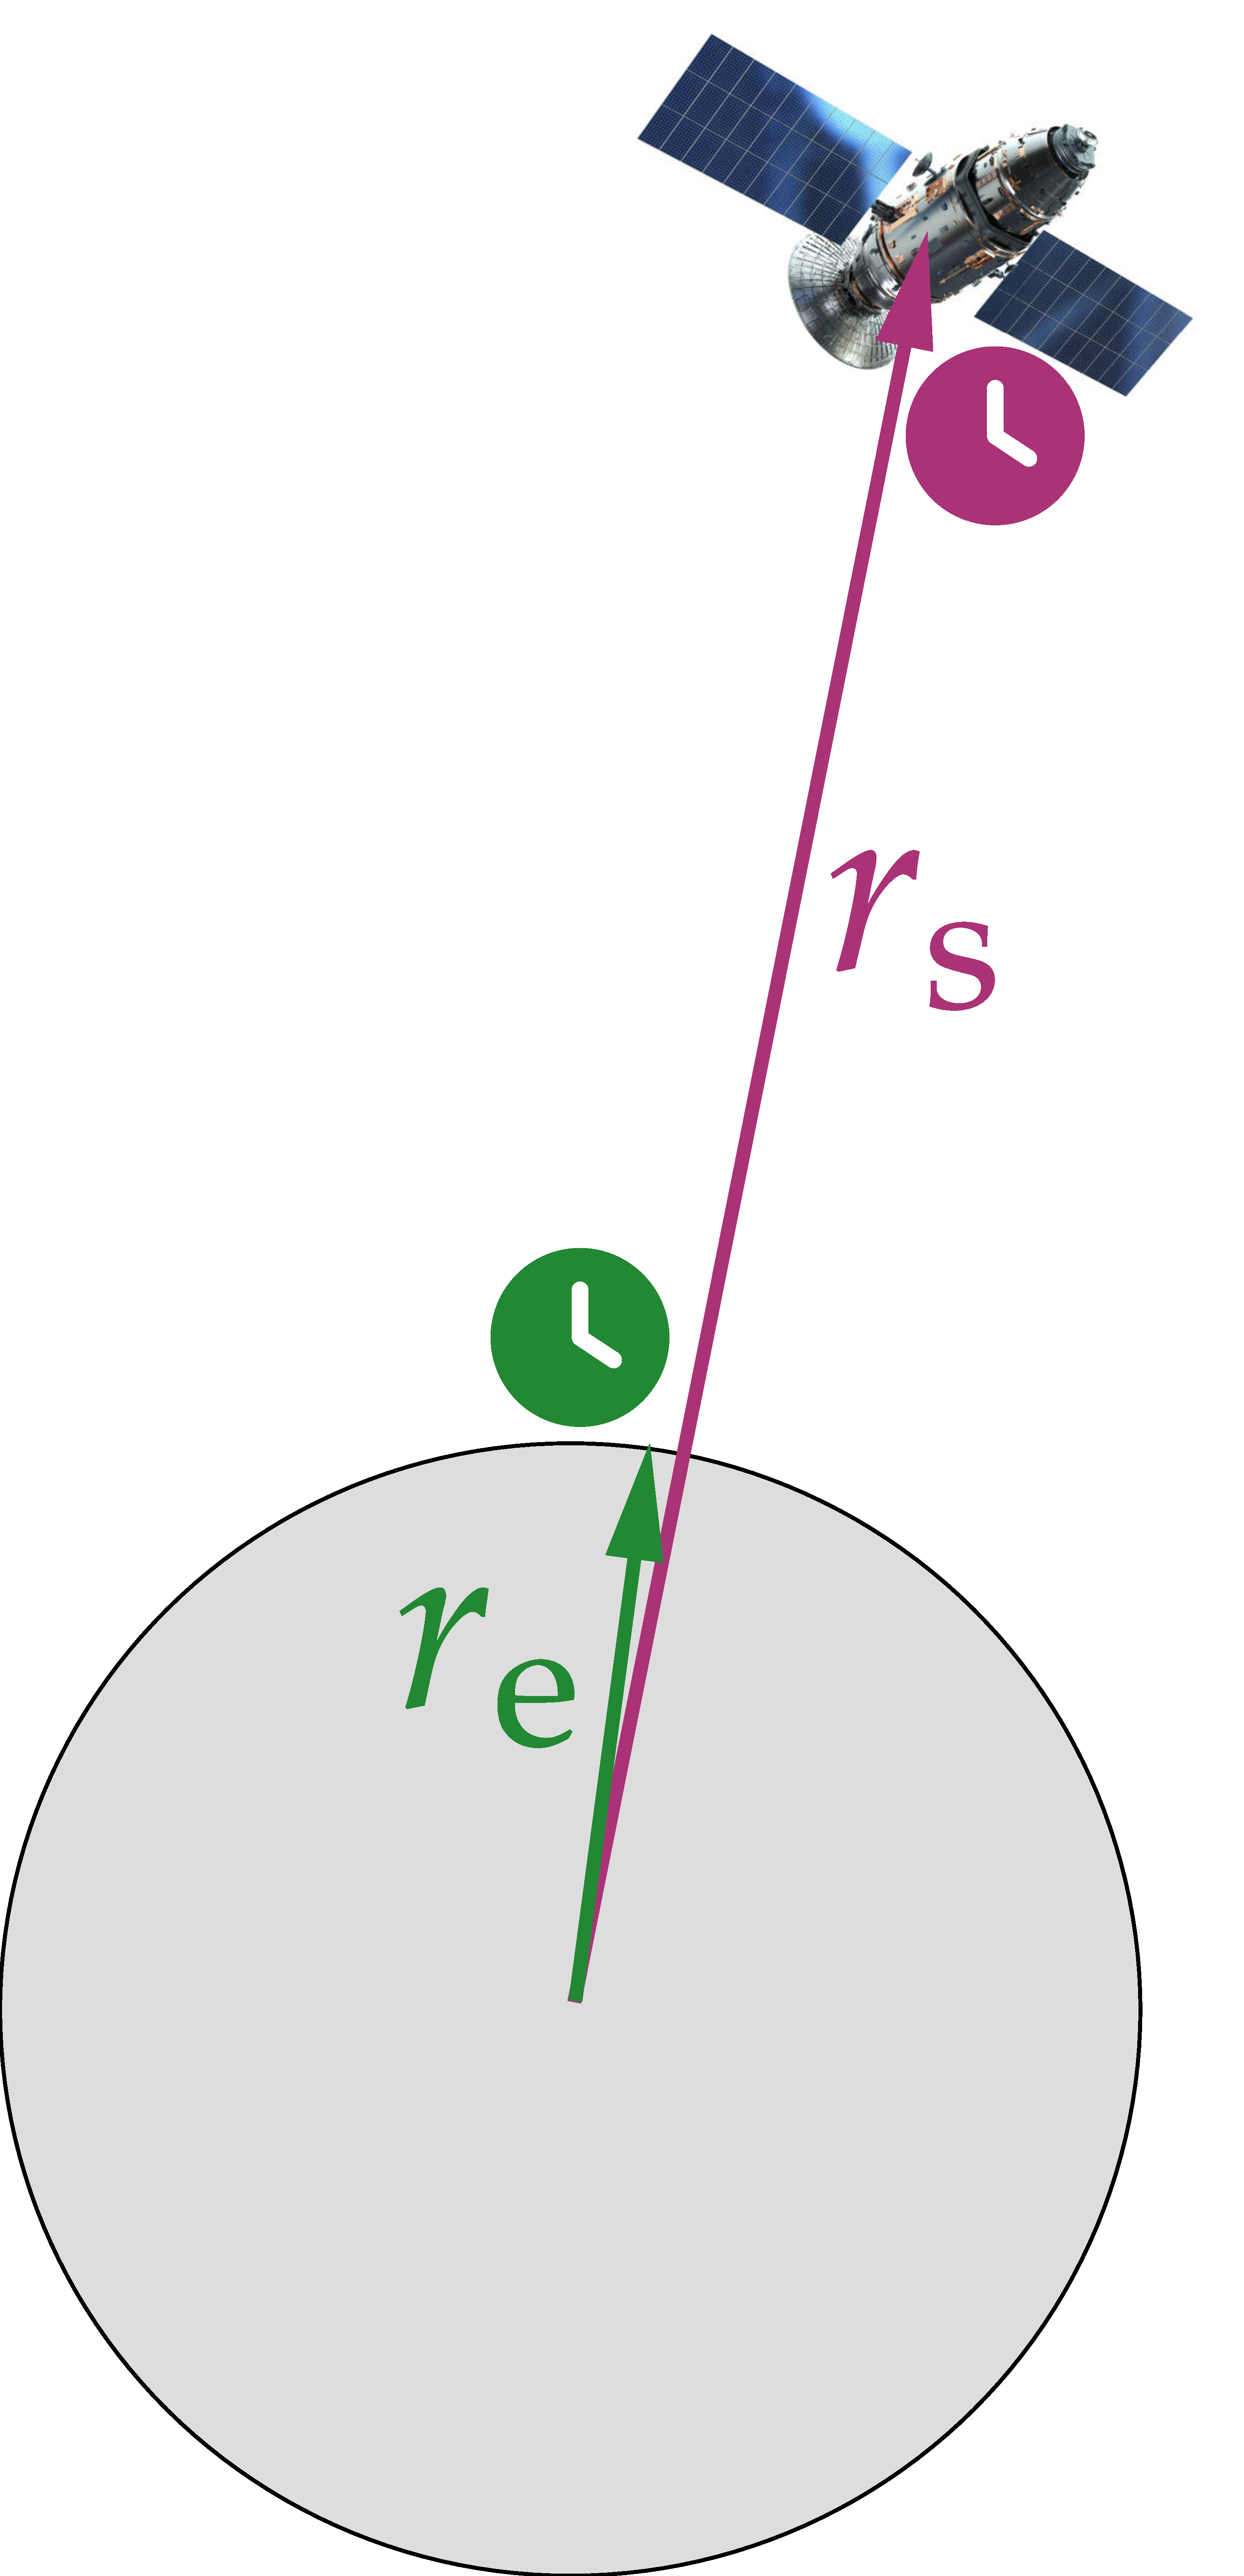
\includegraphics[align=t,width=0.75\linewidth]{re_rs.pdf}
}
\begin{equation*}
  \frac{\Dt_{\text{s}}}{\Dt_{\text{e}}} =
  \frac{
    \sqrt{1-2\frac{G}{c^{2}}\frac{M}{r_{e}}}
  }{
    \sqrt{1-2\frac{G}{c^{2}}\frac{M}{r_{s}}}
  }
\end{equation*}
where $G\approx\qty{6.7e-11}{m^{3}/(kg.s^{2})}$, $c=\qty{3.0e8}{m/s}$, and the Earth's mass $M=\qty{6.0e24}{kg}$.



\begin{enumerate}[shift,label={\bfseries\arabic*.}]
\item Take the case of a GPS satellite, with $r_{\text{e}}=\qty{6.4e6}{m}$ and $r_{\text{s}}=\qty{2.6e7}{m}$ (\furl{https://www.nasa.gov/directorates/somd/space-communications-navigation-program/gps/}{NASA data}). If you, on the ground, measure a time lapse of $\Dt_{\text{e}}=\qty{10}{years}$, what's the difference, in seconds, with the time lapse $\Dt_{\text{s}}$ you see on the satellite?

\item If the time lapses are large compared with the time needed to go from ground to orbit or vice versa, then $\Dt_{\text{s}}/\Dt_{\text{e}}$ is also the ratio between the real \emph{ageing} of a person who's been in orbit and one who's been on the ground, when they meet again.

  Now consider the case with a black hole instead of Earth. The formula above still apply approximately.

  In the movie \furl{https://www.imdb.com/title/tt0816692/}{\emph{Interstellar}}, two
  astronauts go on Miller's planet, at a distance $r_{\text{e}}$ from the black hole Gargantua, and stay there for \qty{3}{hours}, leaving one astronaut in orbit at a distance $r_{\text{s}}\approx \infty$ (the distance is large enough that it can be approximated as infinity). When they meet again, the latter astronaut has aged \emph{23\;years}.
\sidepar{\footnotesize\centering%
\vspace{-7em}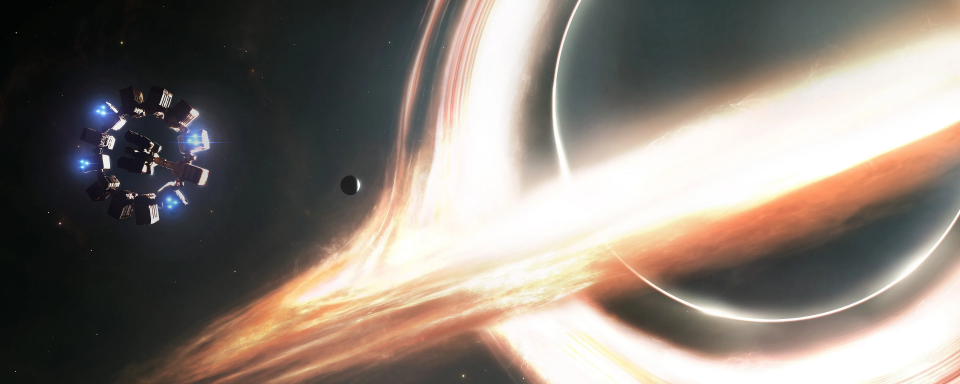
\includegraphics[align=t,width=\linewidth]{gargantua.png}
}

  Given that Gargantua's mass is $M=\qty{2.0e38}{kg}$, calculate the distance $r_{\text{e}}$ of Miller's planet from the black hole.
\end{enumerate}
\end{exercise}




\section{Velocity and acceleration}
\label{sec:velocity}

In some situations the spatial coordinates $\yr=(x,y,z)$ may turn out to be functions of the time coordinate $t$; the typical example is when we describe how the spatial position of a small body changes with coordinate time. We can write this functional dependence in different ways, for instance
\begin{equation*}
  \yr(t)\quad\text{or}\quad
  \bigl[x(t),\ y(t),\ z(t)\bigr] \ .
\end{equation*}
So $\yr$ is a vector function of time, which simply means that we have a collection of three functions of time.

If we take the derivative of each coordinate with respect to the time $t$, we obtain the \textbf{coordinate velocity}
\begin{equation*}
  \yv(t) \defd \frac{\di}{\di t}\yr(t) = \biggl[\frac{\di}{\di t} x(t),\ \frac{\di}{\di t} y(t),\ \frac{\di}{\di t} z(t)\biggr]
\end{equation*}
which is also a vector.

\begin{definition}{Dot-notation for time derivative}
  The derivative of some quantity with respect to coordinate time is often denoted by a \textbf{dot} over the quantity. So we can also write
  \begin{equation*}
    \yv(t) = \dot{\yr}(t) = \bigl[\dot{x}(t),\ \dot{y}(t),\ \dot{z}(t)\bigr]
  \end{equation*}
\end{definition}

The coordinate velocity is usually different from the \emph{physical velocity}, which an observer would measure using proper time and space, for instance using bouncing light rays. In many everyday situations the difference between coordinate and physical velocity is so small that it can be neglected. But in situations involving subatomic particles at high speed, for example, one must take into account that the two velocities are different.

\smallskip

Taking the time derivative once more we obtain the coordinate acceleration, also a vector:
\begin{equation*}
  \bm{a}(t) \defd \frac{\di}{\di t}\yv(t) =
  \frac{\di^{2}}{\di t^{2}}\yr(t) = \biggl[\frac{\di^{2}}{\di t^{2}} x(t),\ \frac{\di^{2}}{\di t^{2}} y(t),\ \frac{\di^{2}}{\di t^{2}} z(t)\biggr]
\end{equation*}
which is also a vector.

\begin{extra}{Acceleration in relativity theory}
  In relativity theory, acceleration acquires a special physical significance, because it includes the effect of gravity, and its calculation does not involve just a time derivative. For instance, let's say that you are standing still on the ground, and let's use a coordinate system where $x$ points in front of view, $y$ to your left, and $z$ points upwards. Then your coordinate velocity is $\yv=(0,0,0)\:\unit{m/s}$ also according to relativity theory. But the spatial part of your acceleration is approximately $(0,0,9.8)\:\unit{m/s^{2}}$, not zero!

  The definitions and values of acceleration according to relativity theory and according to Newtonian mechanics are therefore quite different even in everyday situations. In these notes we'll mean the Newtonian definition of acceleration, unless stated otherwise.
\end{extra}

\medskip

\begin{exercise}
  \begin{enumerate}[shift,label=\bfseries\arabic*.]
  \item Here are the three components of a time-dependent velocity vector; the variable $t$ is the time, and therefore has dimension \textsf{time}. Introduce units \enquote*{\unit{s}} and \enquote*{\unit{m}} appropriately in such a way that the expression is dimensionally correct:
    \begin{equation*}
      \bm{v}(t) = \bigl[4, \cos(3\,t), -\exp(8/t)\bigr]
    \end{equation*}
  \item The position vector of a satellite is given below. Calculate the satellite's velocity and acceleration vectors:
    \begin{equation*}
      \yr(t) =
      \begin{bmatrix}
        \num[exponent-mode=scientific]{20e+6}\,
        \cos\bigl(\frac{t}{\qty{13751}{s}}\bigr)\\[2\jot]
        \num[exponent-mode=scientific]{22e+6}\,
        \sin\bigl(\frac{t}{\qty{13751}{s}}\bigr)\\[2\jot]
        \num{0}
      \end{bmatrix}\:\unit{m}
    \end{equation*}
  \item What is the satellite's velocity at $t=\qty{6875}{s}$? What is the magnitude of the velocity (that is, the speed)?
  \end{enumerate}
  
\end{exercise}

\clearpage


% \begin{subappendices}
% 
% \addsec{\color{green}\faIcon{puzzle-piece}\enspace Exercises\enspace\faIcon{puzzle-piece}}
% 
% % \setsecnumformat{E\upshape\oldstylenums{\csname the#1\endcsname\quad}}
% % \setsecnumformat{\sectionname\
% % \oldstylenums{\csname the#1\endcsname\quad}}
% 
% \exsubsec{\ref{sec:coords}}
% 
% \marginpar{\footnotesize\centering%
%   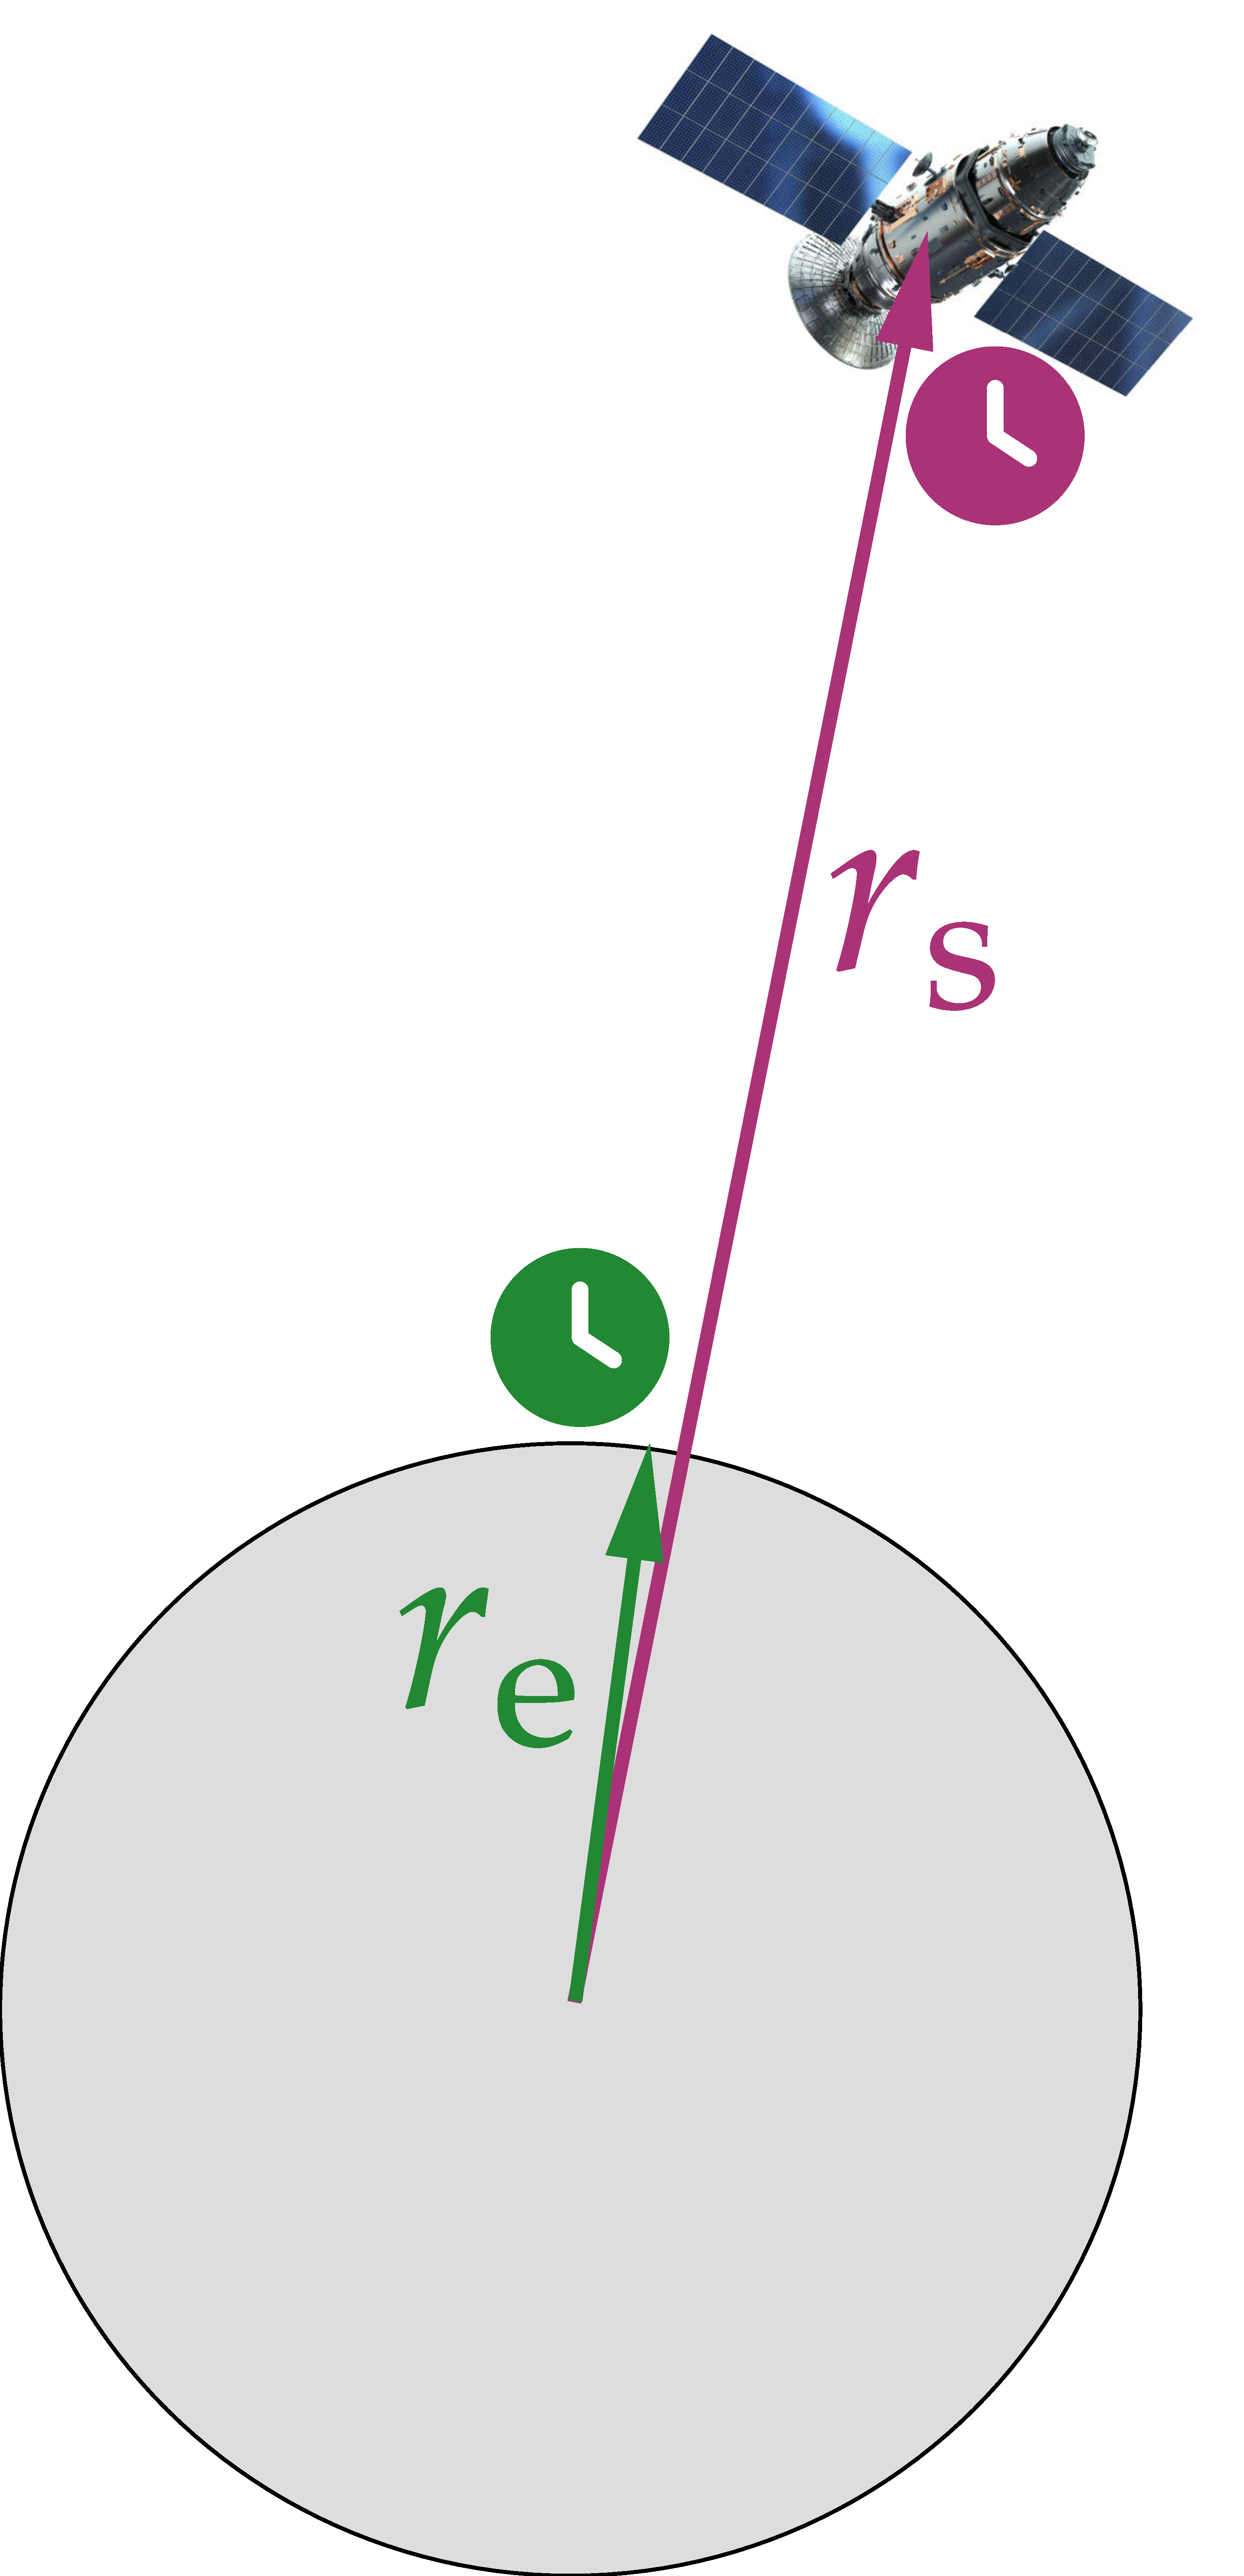
\includegraphics[align=t,width=0.75\linewidth]{re_rs.pdf}
% }
%   Consider a clock at rest on the Earth's surface, at a distance $\color{green}r_{\text{e}}$ from the Earth's centre; and a clock on a satellite, for instance a GPS satellite or the \furl{https://www.nasa.gov/international-space-station/}{International Space Station}, right above the first clock, at a distance $\color{red}r_{\text{s}}$ from the Earth's centre. An observer by the clock on Earth measuring a time lapse $\Dt_{\text{e}}$ will see the clock on the satellite has having run for a time lapse $\Dt_{\text{s}}$, and vice versa (note that this \enquote{vice versa} only holds in this specific situation!). The relation between two time lapses is approximately given by
% \begin{equation*}
%   \frac{\Dt_{\text{s}}}{\Dt_{\text{e}}} =
%   \frac{
%     \sqrt{1-\frac{G}{c^{2}}\frac{M}{r_{e}}}
%   }{
%     \sqrt{1-\frac{G}{c^{2}}\frac{M}{r_{s}}}
%   }
% \end{equation*}
% where $G\approx\qty{6.7e-11}{m^{3}/(kg.s^{2})}$, $c=\qty{3.0e8}{m/s}$, and the Earth's mass $M=\qty{6.0e24}{kg}$.
% 
% 
% \begin{enumerate}[shift,label={\bfseries\arabic*.}]
% \item Take the case of a GPS satellite, with $r_{\text{e}}=\qty{6.4e6}{m}$ and $r_{\text{s}}=\qty{2.6e7}{m}$ (\furl{https://www.nasa.gov/directorates/somd/space-communications-navigation-program/gps/}{NASA data}). If you, on the ground, measure a time lapse of $\Dt_{\text{e}}=\qty{10}{years}$, what's the difference, in seconds, with the time lapse $\Dt_{\text{s}}$ you see on the satellite?
% 
% \item If the time lapses are large compared with the time needed to go from ground to orbit or vice versa, then $\Dt_{\text{s}}/\Dt_{\text{e}}$ is also the ratio between the real \emph{ageing} of a person who's been in orbit and one who's been on the ground, when they meet again.
% 
%   Now consider the case with a black hole instead of Earth. The formula above still apply approximately.
% 
%   In the movie \furl{https://www.imdb.com/title/tt0816692/}{\emph{Interstellar}}, two
%   astronauts go on Miller's planet, at a distance $r_{\text{e}}$ from the black hole Gargantua, and stay there for \qty{3}{hours}, leaving one astronaut in orbit at a distance $r_{\text{s}}\approx \infty$ (the distance is large enough that it can be approximated as infinity). When they meet again, the latter astronaut has aged \emph{23\;years}.
% \sidepar{\footnotesize\centering%
% \vspace{-10em}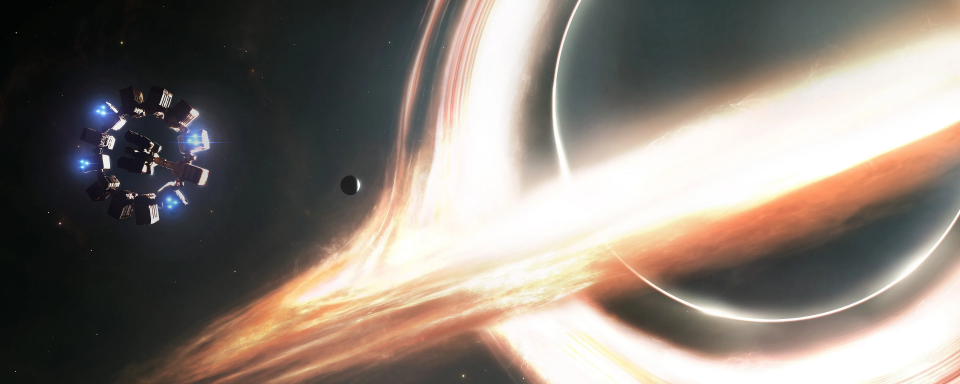
\includegraphics[align=t,width=\linewidth]{gargantua.png}
% }
% 
%   Given that Gargantua's mass is $M=\qty{2.0e38}{kg}$, calculate the distance $r_{\text{e}}$ of Miller's planet from the black hole.
% \end{enumerate}
% 
% 
% 
% \end{subappendices}





\printpagenotes*
\clearpage
\chapter{Building blocks: \enquote{Stuff}}
\label{cha:stuff}

% \epigraph{\emph{For Euler, clarity was the hallmark of truth. \textelp{} To him we owe also the brilliant imagination of the internal pressure in generality, the pressure field as equipollent to the action of the fluid outside any imaginary closed diaphragm upon that within. \textelp{} I remark upon it in emphasis of the role of imagination and the importance of quantities which can only be thought of and cannot in themselves be measured.}}{C. A. Truesdell \cites*{truesdell1956d}}

\epigraph{\emph{if the skill of the mathematician has enabled the experimentalist to see that the quantities which he has measured are connected by necessary relations, the discoveries of physics have revealed to the mathematician new forms of quantities which he could never have imagined for himself.}}{J. Clerk Maxwell \cites*{maxwell1870}}


\section{Seven primitive quantities with three basic properties}
\label{sec:stuff}

Besides time and space, our physics formalism includes around seven more quantities that we take as primitive:
\begin{definition}{Seven primitive quantities}
  \begin{center}\bfseries
    matter
    \\ electric charge
    \\ magnetic flux
    \\ energy
    \\ momentum
    \\ angular momentum
    \\ entropy
  \end{center}
\end{definition}
Technically they are called \emph{fields}, for reasons we shall shortly see.

\medskip

Recall that primitive quantities cannot be defined: we can only try to understand them intuitively, for example through their properties. Some of the seven primitive quantities are easier to grasp intuitively than others. But all seven primitive quantities have three basic properties in common. First of all, of each we can ask, or rather, measure:
\begin{definition}{The two basic measurements that can be made on the seven quantities}
  \begin{enumerate}[shift,label=\arabic*.]\bfseries
  \item How much of this quantity is in a particular three-dimensional region of space at a particular time instant?
    
  \item How much of this quantity flows through a particular two-dimensional surface during a particular time lapse?
  \end{enumerate}
\end{definition}
We can ask these questions of any region of space and any time lapse, and the surface in the second question can be moving and deforming.
% \mynotew{densities and fluxes?}
The results of the two measurements above are numbers, which in general can be positive or negative, for scalar quantities; or vectors for vector quantities.
% This number depends only on the chosen region, surfaces, and times.

Often we consider the second question, about the flow through a surface, in the case of a very short lapse of time, and divide the total flow by that time lapse. So we have an alternative form of the second measurement:
\begin{definition}{Flux of a substance through a surface}
  \begin{enumerate}[shift,label=\arabic*.]\bfseries
  \item[2b.] How much of this quantity is flowing through a particular two-dimensional surface per unit time, at a particular time instant?
  \end{enumerate}
\end{definition}
This is called the \textbf{flux} of the quantity through that surface.

The third  property common to the seven quantities regards the two measurements above.
\begin{definition}{Extensivity of the seven quantities}\label{def:extensivity}
  If we consider two or more separate volumes, the amount of quantity in the total volume is equal to the sum of the amounts in the separate volumes.

  Analogously for the flux through separate surfaces.
\end{definition}
We say that each of the seven quantities is an \textbf{extensive} quantity

\smallskip

The basic measurements above can't in general be made, and don't even make sense, for some other quantities. For instance, we cannot ask \enquote{what's the total amount of \emph{temperature} in this region?}, or \enquote{how much velocity is flowing through this surface?}.

\smallskip

Thanks to the three properties above, each of the seven quantities can be intuitively visualized as some kind of \enquote{stuff} that can be present at each spacetime point, fills regions of space, and flows through surfaces. This visualization is useful, but also comes with some warnings which we'll discuss later.
% But don't take the word \enquote*{stuff} too literally: I don't necessarily mean concrete objects like a ball, or substances like water.

% For each quantity, we can speak of its \emph{density}, in relation to the question \enquote{how much of it is in a particular region?}; and of its \emph{flux}, in relation to the question \enquote{how much of it flows through a surface during some time?}. The density tells us how much quantity there's in a unit of volume. The flux tells us how much quantity is flowing through a unit of surface in a unit of time. Density and flux can change from spacetime point to spacetime point. We shall discuss them more in detail for each quantity later on. One important aspect to keep in mind is that \emph{the density and flux of each quantity depend on the coordinate system}.

\smallskip

What's remarkable about matter, electric charge, magnetic flux, energy, momentum, angular momentum, and entropy, is that \emph{they are common to all our main physical theories}, approximate or not: from Newtonian mechanics to general relativity and quantum theory; from subatomic scales to cosmological scales. The physical meaning and mathematical characterization of these quantities can be slightly different depending on the physical theory and scale. For example, in quantum theory they are mathematically represented by so-called operators rather than functions; and at molecular scales entropy has a meaning connected with probability theory. Yet, these seven quantities are really universal to our present way of doing physics and of describing physical phenomena around and within us.

% \begin{critique}
%   \emph{Wait! what about \emph{force}? isn't this a primitive quantity? or maybe it isn't included because it's defined as mass${}\times{}$acceleration?}
% 
%   \smallskip
% 
% We'll see that \emph{force} is defined as momentum flux; but that in general isn't mass${}\times{}$acceleration.
% \end{critique}

Let us make a first acquaintance with these seven quantities. The discussion that follows is meant as an introduction; we shall repeat and say more about each quantity in later chapters.

\marginpar{\centering%
\href{https://www.youtube.com/watch?v=nYg6jzotiAc&t=893s}{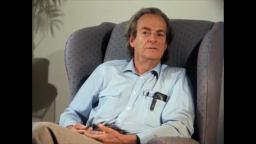
\includegraphics[align=c,width=\linewidth]{feynman_why2.png}}%
\\[\jot]\footnotesize\flushleftright{\color{mpcolor}%
Richard Feynman explains the difficulty of \enquote{why} questions in a \furl{https://www.youtube.com/watch?v=nYg6jzotiAc&t=893s}{funny and insightful video}.}%
}%
Keep in mind that it is very difficult, if not impossible, to answer questions like \enquote{what \emph{really} is\textellipsis?} or \enquote{why \emph{really} does\textellipsis?}.

\section{Matter}
\label{sec:intro_matter}

Matter is a \emph{scalar} quantity, with SI dimension \furl{https://doi.org/10.1351/goldbook.A00297}{\textsf{amount of substance}}, and measured in units of \furl{https://doi.org/10.1351/goldbook.M03980}{\emph{moles} (\unit{mol})}. Its flux is therefore measured in units of \emph{moles per second} (\unit{mol/s}). In statistical mechanics and particle physics, matter is often simply counted and so measured in dimensionless units, rather than moles.

Matter is probably the easiest quantity to grasp intuitively; what we ordinarily call \enquote{stuff} is matter. % It is called \furl{https://doi.org/10.1351/goldbook.C01039}{\emph{chemical substance}} in chemistry, and \emph{baryons} and \emph{leptons} in particle physics.
It is usually classified into several kinds; the classification depends on the physical phenomena and physical theory one works with, and is related to whether the kinds of matter can be considered separately conserved, as we'll discuss in \chap\,\ref{cha:cons_matter}.

In everyday phenomena not involving \furl{https://www.iaea.org/newscenter/news/what-are-radioactive-sources}{radioactivity}
% \url{https://www.britannica.com/science/radioactivity}
or \furl{https://www.iaea.org/newscenter/news/what-is-nuclear-energy-the-science-of-nuclear-power}{nuclear energy},
% \url{https://www.britannica.com/science/nuclear-fission}
the different kinds of matter approximately correspond to the non-\furl{https://www.ciaaw.org/radioactive-elements.htm}{radioactive chemical elements}: \furl{https://pubchem.ncbi.nlm.nih.gov/element/Hydrogen}{hydrogen}, \furl{https://pubchem.ncbi.nlm.nih.gov/element/Helium}{helium}, \furl{https://pubchem.ncbi.nlm.nih.gov/element/Lithium}{lithium}, and so on. %\furl{https://doi.org/10.1351/goldbook.C01022}{}.
Note that some common everyday devices, such as smoke detectors, do involve radioactivity.

In phenomena involving radioactivity or nuclear energy, the different kinds of matter correspond approximately to \furl{http://hyperphysics.phy-astr.gsu.edu/hbase/Particles/hadron.html\#c6}{\emph{baryons}},
% \url{https://www.britannica.com/science/baryon}},
such as protons and neutrons; and \furl{http://hyperphysics.phy-astr.gsu.edu/hbase/Particles/lepton.html\#c1}{\emph{leptons}},
% \url{https://www.britannica.com/science/lepton}},
such as electrons. In particle physics, even more subtle classifications of matter are made, into kinds that seem to be conserved, such as electronic-leptons, muonic-leptons, and others. This kind of research is still open, but it seems that the total amount of baryonic and leptonic matter, independently of the kinds into which it can be classified, is always conserved. Note that we're using the term \enquote*{matter} in a sense that includes anti-matter, such as positrons.

The total amount of matter in a region \emph{can be negative}. \enquote{Negative matter} is what's usually called \furl{https://www.britannica.com/science/antimatter}{anti-matter}. Anti-matter appears in small amounts in everyday life, for example in connection with common radioactivity processes. It is also created and used in medicine, in \furl{https://www.britannica.com/topic/positron-emission-tomography}{positron-emission tomography (PET)} scans.

In these notes we shall usually not consider distinctions between different kinds of matter, making some exceptions for discussions about chemical reactions and nuclear phenomena.

% There are different kinds of matter The distinction into different kinds depends on the physical theory. In most everyday situations, the distinction corresponds to different \furl{https://doi.org/10.1351/goldbook.C01022}{chemical elements}, and each satisfies its own balance. These balances are the basis of \furl{https://doi.org/10.1351/goldbook.S06026}{stoichiometry}. If we observe phenomena such as nuclear fission or fusion, however, we notice that the balances of chemical elements are not really satisfied. With such phenomena we make a different distinction of types of matter, for instance \emph{baryons} and \emph{leptons}, and each satisfies again its own balance. It is unclear whether these balances might be broken in other physical phenomena at smaller scales. In these notes we shall usually consider chemical elements as the different kinds of matter, making some exceptions in discussion of nuclear phenomena.

\begin{definition}{Matter: notation}
  The amount of matter in a region is usually denoted with $\yN$, and flux of matter with $\yJ$. In chemistry we usually specify what kind of matter we are speaking about, writing for instance $\yN_{\mathrm{Ca}}=\qty{5.3}{mol}$, to indicate an amount of $\qty{5.3}{mol}$ of \furl{https://pubchem.ncbi.nlm.nih.gov/element/Calcium}{calcium} atoms.
\end{definition}

\begin{warning}[Matter is different from mass or energy]
  It is important to clearly distinguish matter from \emph{mass} or \emph{energy}. Mass can be considered a property of matter, but the two are different. In nuclear reactions, for instance, the mass of some amount of matter may change, even if the amount of matter stays the same.

  \smallskip

  As far as we know, the total amount of energy associated with an amount of matter is always positive, whether the amount of matter is positive or negative (antimatter). This is the reason why antimatter \enquote{falls} just like positive matter, a fact that has been experimentally confirmed: see \cites{andersonetal2023}.
\end{warning}

\begin{exercise}
  According to statements on \furl{https://www.symmetrymagazine.org/2009/07/23/antimatter-from-bananas}{symmetrymagazine.org} and \furl{https://www.quantumdiaries.org/2009/07/21/positrons-from-bananas/}{quantumdiaries.org},
  \begin{quote}
    The average banana (rich in potassium) produces a positron roughly once every 75 minutes.
  \end{quote}
  Unfortunately the original site where the this statement was discussed, and the corresponding calculation made, seems not to exist anymore.

\begin{enumerate}[shift,label=\arabic*.]\bfseries
\item Do a little research and find out whether this statement is true.
\item From your research, approximately quantify the flux of positrons around an ordinary banana, expressing it in \unit{particles/s}.
\end{enumerate}
\end{exercise}
\marginpar{\vspace{-15em}\footnotesize%
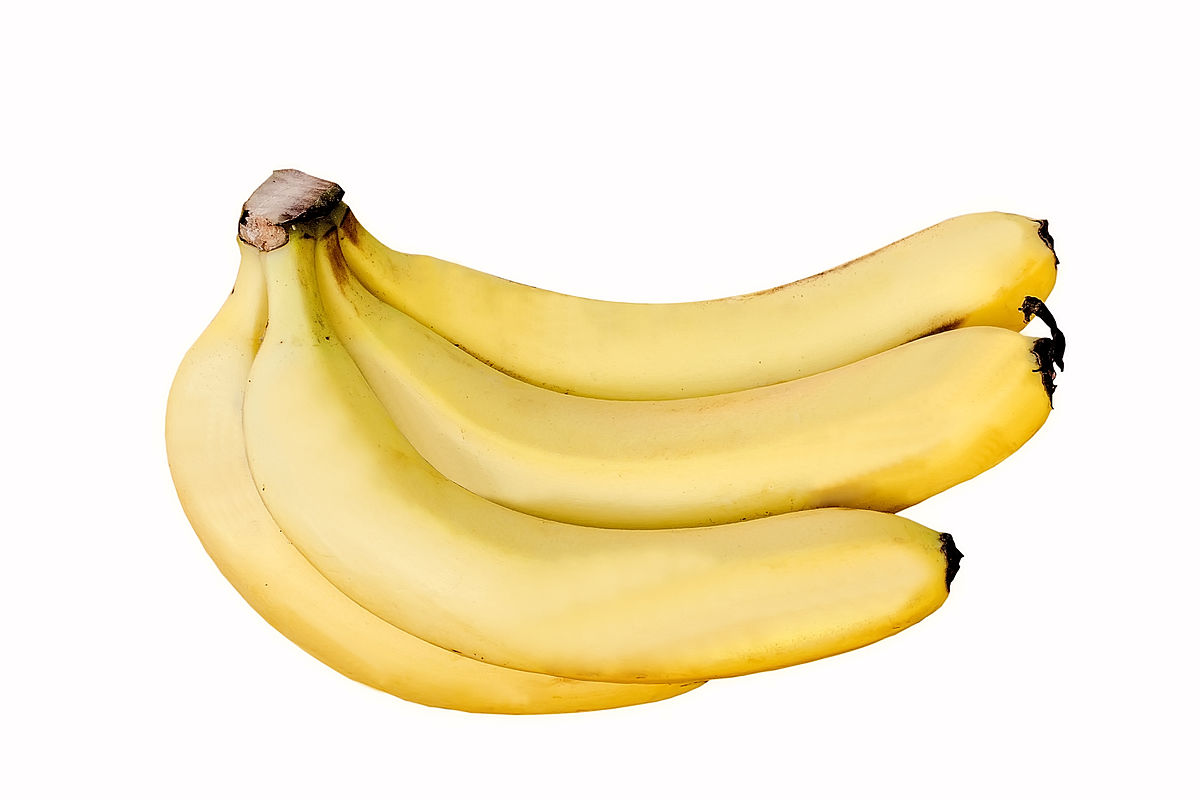
\includegraphics[align=b,width=\linewidth]{banana.jpg}
\\{\color{mpcolor}How many positrons do bananas produce?}
}



\section{Electric charge and magnetic flux}
\label{sec:intro_charge}

Electric charge is a \emph{scalar} quantity, with SI dimension \furl{https://doi.org/10.1351/goldbook.E01923}{\textsf{electric charge}} (equivalent to \textsf{electric current}$\times$\textsf{time}), and measured in units of \furl{https://doi.org/10.1351/goldbook.C01365}{\emph{coulombs} (\unit{C})}. Flux of electric charge is called \emph{electric current}, and measured in units of \furl{https://doi.org/10.1351/goldbook.A00300}{\emph{amperes} ($\unit{A} = \unit{C/s}$)}.

Electric charge is a quantity that is easily grasped in our everyday experience, and doesn't need much comments.

\bigskip

\marginpar{\footnotesize%
%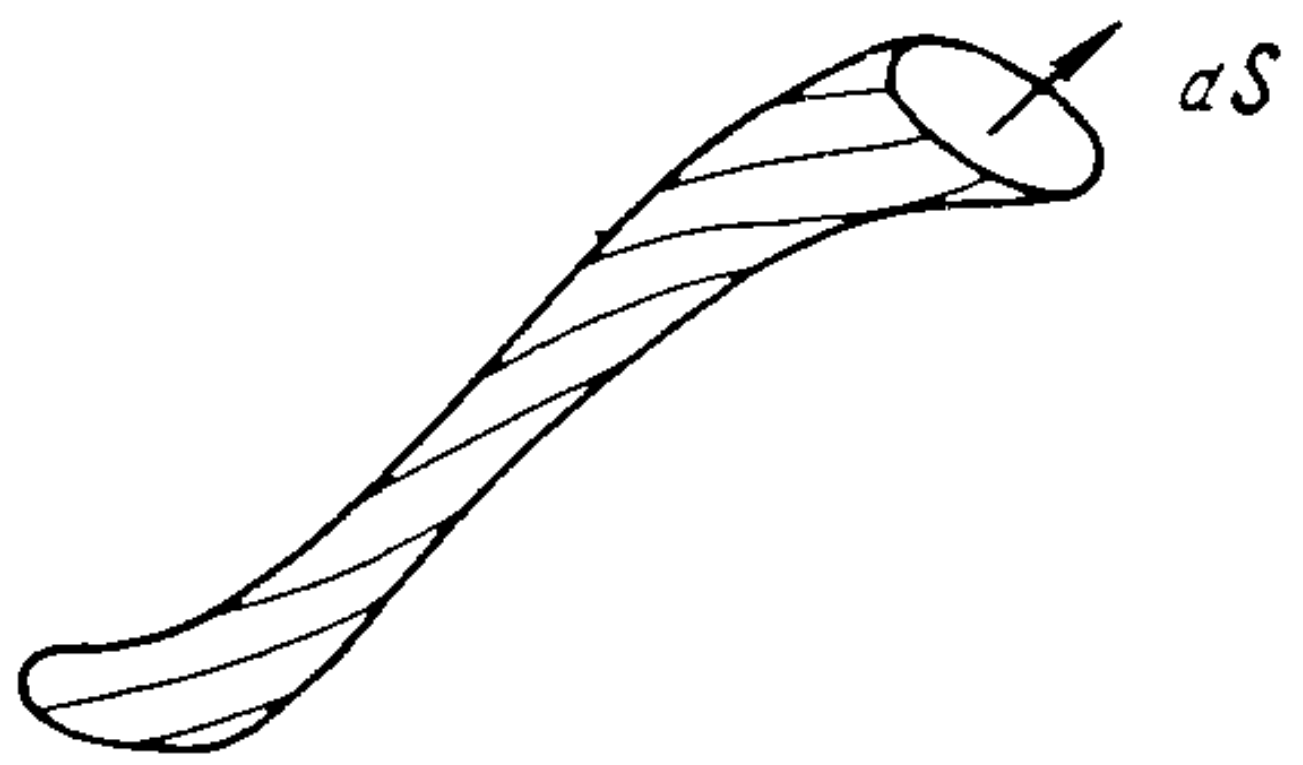
\includegraphics[align=t,width=\linewidth]{magnflux1.png}
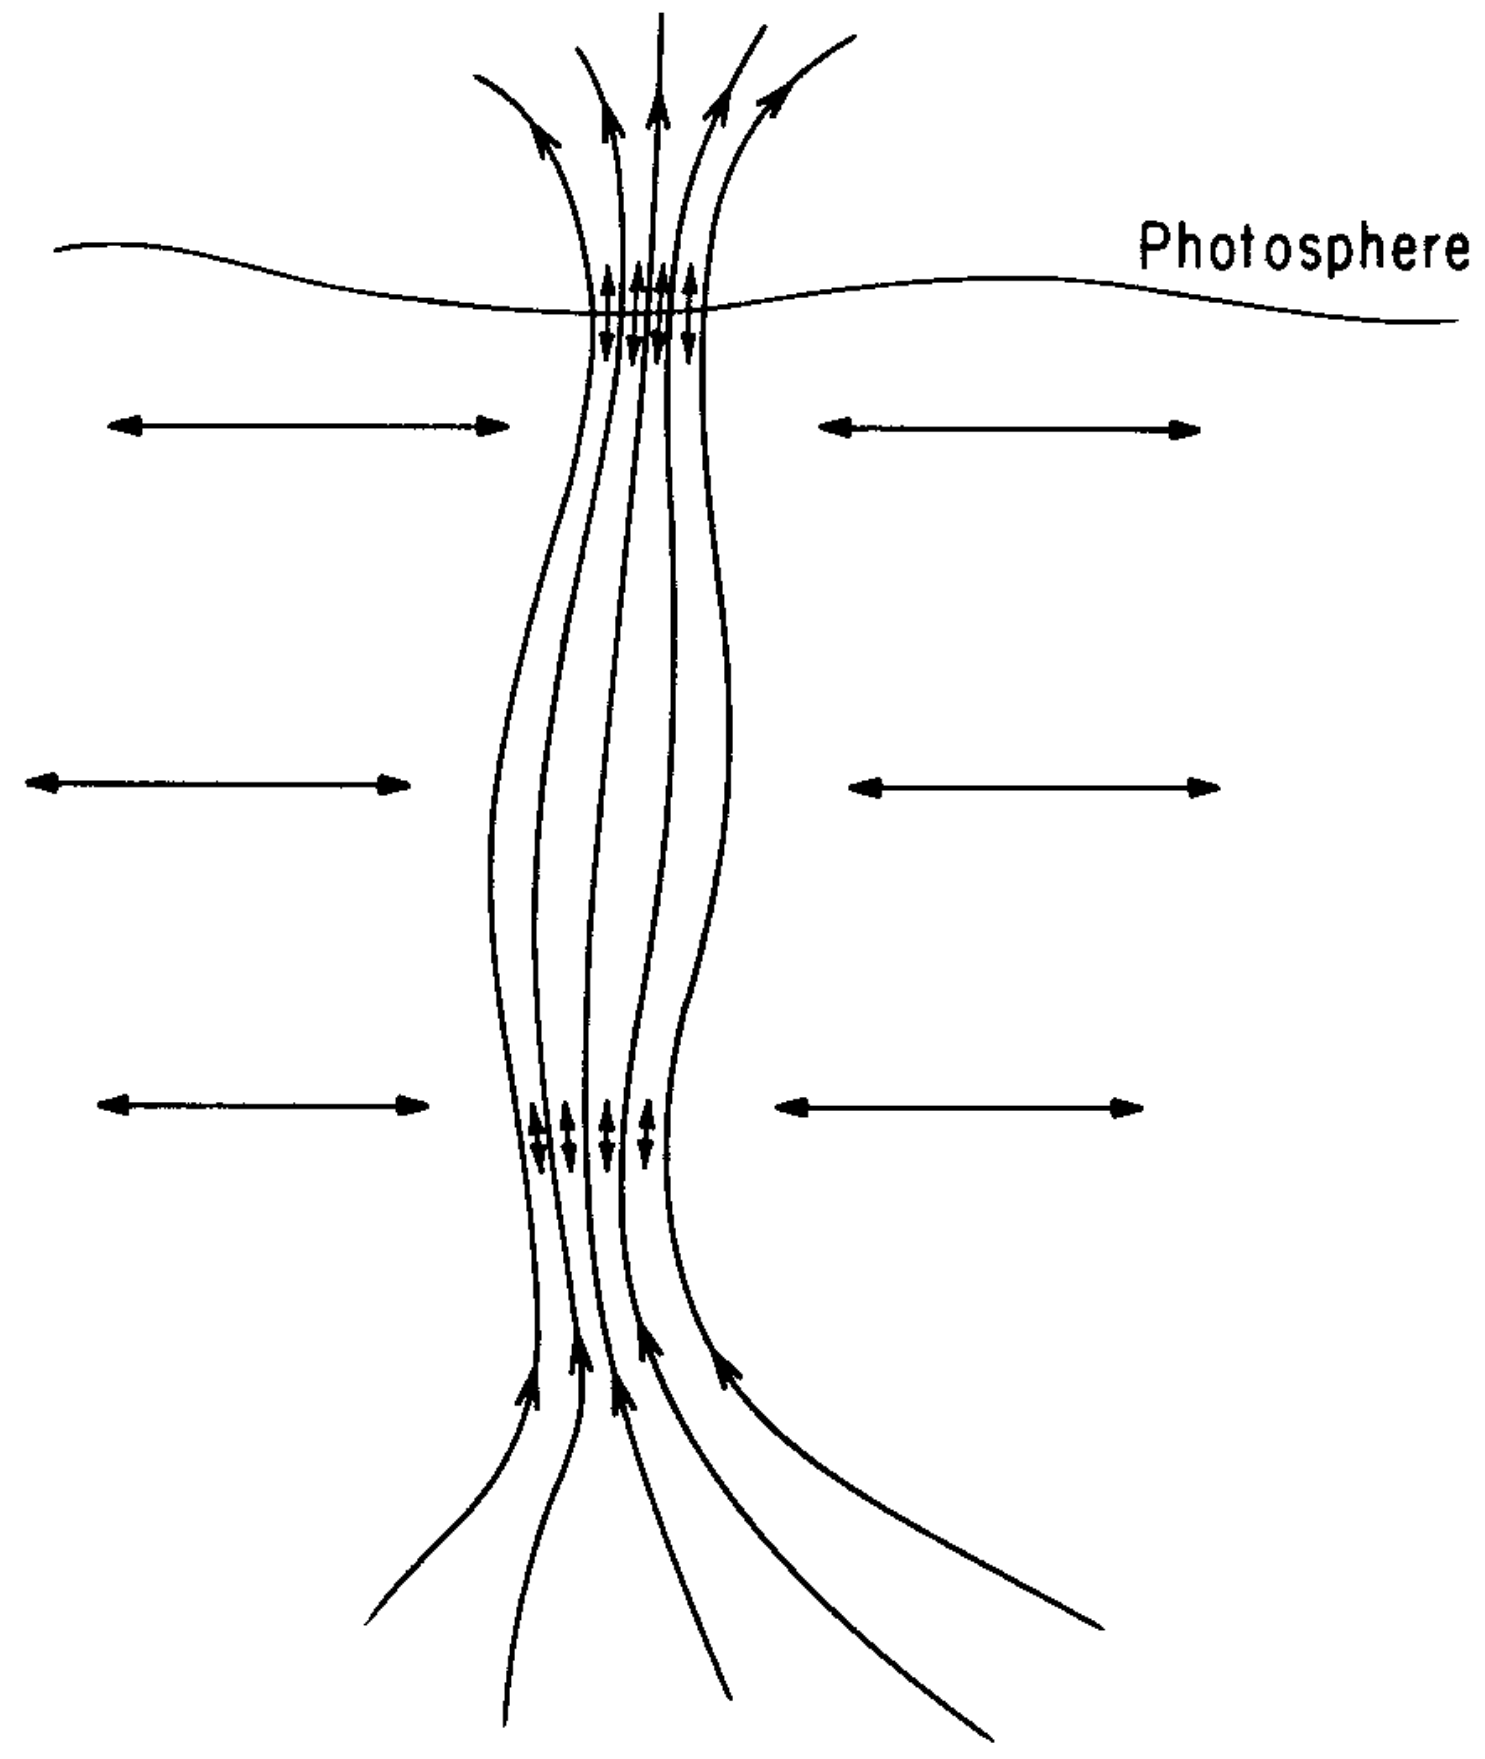
\includegraphics[align=t,width=\linewidth]{magnflux2.png}
\\{\color{mpcolor}\enquote{\emph{%
sketch of the magnetic lines of force in a magnetic filament extending up through the photosphere.}}\sourceatright{\cites{parker1974b}}}
}
Magnetic flux is a \emph{vector} quantity, with SI dimension \furl{https://doi.org/10.1351/goldbook.M03684}{\textsf{magnetic flux}}, and measured in units of \furl{https://doi.org/10.1351/goldbook.W06666}{\emph{webers} (\unit{Wb})}.


The electromagnetic field
is most commonly represented by vectors associated to each point in space.
But it can also be interpreted and visualized as a collection of moving, oriented tubes or lines, either closed or extending indefinitely; somewhat analogously to how we visualize matter and charge, as moving blobs or points, but with one more dimension.
This interpretation goes back to Faraday \parencites*{faraday1846}, Maxwell \parencites*{maxwell1855b}, and later Dirac \parencites*{dirac1955} among others, and today is conveniently used in some fields such as \furl{https://doi.org/10.1093/acrefore/9780190871994.013.21}{solar physics}, for example to study \furl{https://spaceplace.nasa.gov/solar-activity/}{sunspots} (see Ryutova \cites*{ryutova2015_r2018}). From this point of view, the \emph{voltage} turns out to be the flux of the magnetic flux; it is indeed measured in \emph{volts} (\unit{V}), equivalent to \emph{webers/second}.

Electromagnetism and this particular visualization of it are very fascinating topics, but we shall not discuss them in these notes.


\section{Energy}
\label{sec:intro_energy}

Energy is a \emph{scalar} quantity, with SI dimension \textsf{energy}, and measured in units of \emph{joules} (\unit{J}); its flux is measured in units of \emph{watts} ($\unit{W}=\unit{J/s}$).

Equivalently we can speak of mass, with SI dimension \textsf{mass}, and measured in units of \furl{https://doi.org/10.1351/goldbook.K03391}{\emph{kilograms} (\unit{kg})}; its flux is measured in \emph{kilograms per second} (\unit{kg/s}).

\marginpar{%
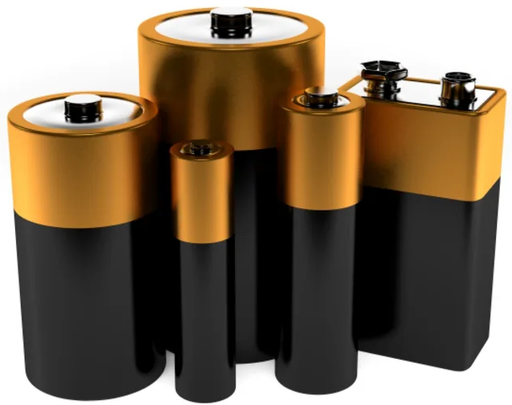
\includegraphics[align=t,width=\linewidth]{batteries.png}
}
The notion of energy is extremely important today, and central in many world-wide important discussions and worries -- think of the \enquote{energy crisis}, \enquote{renewable energy}, and so on. It is somewhat funny that despite this importance it's actually difficult to answer \enquote*{what \emph{is} energy, really?}. Often we speak about energy as something that \enquote{flows}, is \enquote{transported}, \enquote{converted}, \enquote{stored}, and similar visualizations. This intuition will be enough in these notes. The notion of \emph{mass} is also very intuitive in our everyday life; we associate it with the difficulty in setting objects into motion, or with the weight of objects.
% relativity says that there's a strong connection between these two associations.

From Relativity Theory and experimentally we know that \emph{energy and mass are the same quantity}, and in these notes we shall emphasize this experimental fact.


\subsection{Energy and mass are the same}
\label{sec:mass_is_energy}

Let's see some examples of why it is impossible to make a real distinction between energy and mass. The following examples have been simplified in some of their aspects, but their main point is valid.

\paragraph{Heated gas}

Imagine we have a box with a given amount of gas, say \qty{1}{mol} of \furl{https://pubchem.ncbi.nlm.nih.gov/element/Oxygen}{oxygen} molecules. Using an extremely precise weighing scale, we observe that the mass of the gas is, say, exactly
\begin{equation*}
  \qty{0.031999540000000000}{kg} \ .
\end{equation*}
Now we heat the gas, providing \qty{60}{J}, while making sure that not a single molecule of oxygen gets in or out of the box. The temperature of the gas increases by around \qty{3}{K}. We observe that the weight measured by the scale increases while we heat the gas, reaching the new value
% cp= 29.4 J/mol/K  cv=21.1
\begin{equation*}
  \qty{0.031999540000000668}{kg} \ .
\end{equation*}
Clearly the mass has increased, but no molecules were added! The additional mass is the \qty{60}{J} that we provided to the gas. Energy has weight, energy is mass.

% Some texts say that \enquote{mass is a form of energy}, but that's incorrect: mass \emph{is} energy, and energy in all its possible forms \emph{is} mass.

\paragraph{Stretched or moving rubber band}

Take a common rubber band, and imagine again that we have an extremely precise weighing scale. The rubber band, unstretched, has a mass of exactly
\begin{equation*}
  \qty{0.000500000000000000000}{kg}\ .
\end{equation*}
Now we stretch the band a little. According to Newtonian mechanics it acquires \enquote*{elastic energy}, which increases its initial internal energy by, say, \qty{0.3}{J}.
% Refer later to elastic constant
% 0.5 * 50 N/m * (0.1 m)^2 \approx 0.3 J
Now we weigh the rubber band again, while stretched, and observe a mass of approximately
\begin{equation*}
  \qty{0.000500000000000003338}{kg} \ .
\end{equation*}
The extremely small difference of around \qty{3e-18}{kg} from the initial mass
is exactly the elastic energy that we provided by stretching.
\marginpar{%
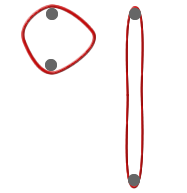
\includegraphics[align=b,width=\linewidth]{rubberbands.png}
\\[\jot]%
{\footnotesize\color{mpcolor}When we stretch a rubber band, its mass increases slightly -- even if the amount of rubber remains exactly the same.\par}
}
Energy has weight; energy is mass.

Now set the unstretched band in motion, so that according to Newtonian mechanics it acquires a kinetic energy of, say, \qty{0.2}{J}. If we could weigh the band while in motion (but without moving the weighing scale), we would measure a mass of approximately
$$\qty{0.000500000000000002225}{kg} \ .$$
The small difference from the initial mass is the new kinetic energy of the band.

This case is actually connected with the example of the gas above. If we observed the gas at a molecular level, we would interpret the energy of \qty{60}{J} provided to it as additional kinetic energy of its molecules. The increase in weight was exactly this additional kinetic energy.

\paragraph{Fission and atomic bombs}
\marginpar{%
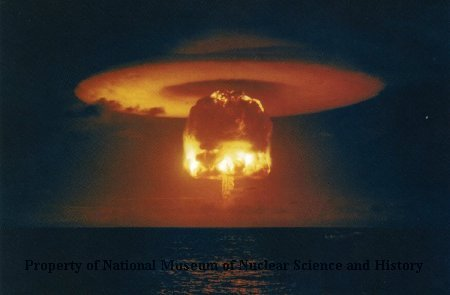
\includegraphics[align=t,width=\linewidth]{atomicbomb.jpg}
\\[\jot]%
{\color{mpcolor}\footnotesize\emph{Hydrogen Bomb Test, 1954%
}\\{(\furl{https://nuclearmuseum.pastperfectonline.com/Archive/716477C1-5E7A-485C-8BE1-857919471563}{National Museum of Nuclear Science \amp\ History})}\par}
}
The \furl{https://www.britannica.com/science/nuclear-fission}{atomic bomb} is a dark example of the fact that mass is energy.
In the case of nuclear fission, if we weigh the amount of nuclear material, say within a box, before and after fission, we observe that its mass has decreased. But we also observe that a great amount of energy has been released out of the box.

\paragraph{Electric heater}

As a final example consider a \qty{1000}{W} electric heater, which is radiating \qty{1000}{J} in one second. The heater is also losing around \qty{0.00000000000001}{kg} of mass every second owing to this heat radiation -- although it's also acquiring the same amount of mass as electromagnetic energy.


\medskip

\marginpar{%
\footnotesize{\color{mpcolor}\enquote{\emph{%
we are led to the more general conclusion: The mass of a body is a measure of its energy content; if the energy changes by $L$, the mass changes in the same sense by $L/9\!\cdot\!10^{20}$, if the energy is measured in ergs and the mass in grams.
%\par Perhaps it will prove possible to test this theory using bodies whose energy content is variable to a high degree (e.g., salts of radium).
}}\sourceatright{\cites{einstein1905d}}}
}
The equivalence between energy and mass is given by the famous formula $E=m c^{2}$, where $c$ is the speed of light, \eqn~\eqref{eq:c}. In their respective units this gives
\begin{equation*}
  \begin{gathered}
    \qty{1}{kg} = \qty{89875517873681764}{J}\quad\text{(exactly)}
    \\
    \qty{1}{J} \approx \qty{0.0000000000000000111265}{kg}
  \end{gathered}
\end{equation*}
To grasp these numbers, consider that the mass of the rubber band in the example above, \qty{0.5}{g}, is comparable to the energy released by the \furl{https://www.britannica.com/story/atomic-bombing-of-hiroshima}{atomic bomb over Hiroshima}.

\subsection{The practical used of the words \enquote*{mass} and \enquote*{energy}}
\label{sec:dist_mass_energy}

From the examples above it becomes clear that energy and mass are two names for the same thing. But it also becomes clear that in our daily experience we deal with energy-mass in two different ways:

On the one hand, we deal with huge (atom-bomb-like) amounts of energy packed in very small volumes: the huge amount of energy that goes together with objects such as pens, keys, bicycles, cars, houses, and so on. We move, push, pull these huge energy amounts from one place to another, and even put them in our pockets. These energy amounts change a little all the time; see the examples above. But the change is so small as to be often undetectable with ordinary scales, and negligible for practical purposes. We call this energy \enquote*{mass} and measure it with a unit -- \unit{kg} -- that doesn't lead to ridiculously large numbers. And we also agree to neglect the imprecision and fluctuation in its measurement, say any imprecision under \qty{0.000001}{\percent}. % This situation is similar to our measuring the power produced by power plants in megawatts (MW). We can say that another power plant constantly produces \qty{500}{MW}; but with this we don't really mean that it produces \emph{exactly} \qty{500000000.000}{W}: there are fluctuations all the time. And we can say that a power plant produces twice as much power, \qty{1000}{MW}, again with the understanding that the ratio is not \emph{exactly} \num{2.000000000000}.

On the other hand, we also deal with the small energy changes and exchanges in all these objects. These exchanges that are very important for our daily life: they keep us warm, make our cells work, make our laptops work. In dealing with these energy exchanges, we don't care about the huge energy reservoirs they come from. So we agree to measure them with a unit -- \unit{J} -- that doesn't lead to ridiculously small numbers. And we also agree not to be precise about the total amount in the reservoir from which these energy bits come from.

As an analogy, consider when we speak about the amount of people in different countries. We can say that in Norway there are \num{5} millions, and in India \num{1500} millions, so in India there are \num{300} times more people. By this we don't mean that in Norway there are \emph{exactly} \num{5000000} people and that India has \emph{exactly} \num{300.000000} times more people. These numbers are changing slightly all the time; but we don't care about differences of 10 or even \num{10000} people. At the same time, think of when you have three dear friends or relatives visiting you from abroad: the amount of \num{3} people is now for you very important; and you don't care about how much this amount is compared to the total population of your country.

\smallskip

The distinction above is of course not clear-cut. In dealing with some physical phenomena, for example with few molecules or in particle physics, the distinction become too blurry and not useful anymore. And indeed in these situations one often uses the terms \enquote*{mass} and \enquote*{energy} interchangeably, as well as a common unit for both (for instance \furl{https://home.cern/tags/13-tev}{\emph{electronvolts}}).

\medskip

% From the examples above it is clear that the energy changes that we deal with and use in everyday situations are extremely small changes in mass -- so small that we can't measure them within the precision of ordinary weighing scales. Vice versa, the masses that we ordinarily deal with are huge amounts of energy. If we spoke only of \enquote*{energy} or only of \enquote*{mass} in all situations, and used only one unit, either joules or kilograms, we would have to work with very impractical numbers. \enquote*{Mass} can be considered a convenient term for \enquote*{energy} when huge amounts of it are involved, concentrated in small regions of space, and ordinary small energy changes can be neglected.
In these notes we shall often use the expressions \enquote*{\energym} and \enquote*{\masse} to remember that these two words denote the same thing.

\subsection{Different \enquote*{forms} of energy}
\label{sec:forms_energy}

We often speak of different \emph{forms} of \energym. The most important for us will be \textbf{internal energy}, \textbf{kinetic energy}, \textbf{gravitational potential energy}, to be discussed later; another important one is \emph{electromagnetic energy}.

In \chap\,\ref{cha:laws} we shall see that the differences among these energy forms come from the way they are calculated from other quantities, such as matter or magnetic flux and electric charge. For example, if we know that in a volume there's an amount of a particular kind of matter, then we know that there must also be an amount of energy given by a particular formula. And if that matter is moving, then we have to add to the total an extra amount of energy given by another formula. And if in that volume there's a gravitational field (that is, a particular kind of spacetime curvature), then another extra amount must be added, given by yet another formula. Similarly if we know that an electromagnetic field is in that volume.

We also speak of different forms of flux of energy. The most important for us will be \textbf{heat} and \textbf{work}, and possibly \textbf{convection}. The difference is again in how these fluxes are calculated depending on whether there are also fluxes of matter.

\subsection{Amounts and forms of energy are coordinate- and observer-dependent}
\label{sec:energy_coords}

An aspect of energy that must always be kept in mind is that \textbf{the amount of energy depends on the coordinate system we're using}. If someone points at a specific region of space at a particular instant, and asks \enquote{how much energy is there?}, we \emph{cannot} give an answer until a coordinate system is specified. Once the coordinate system has been chosen, then a precise and unambiguous answer can be given. The same is true for the flow of energy through a surface. This also means that observers using different coordinates will usually assign different amounts of energy to the same regions of spacetime.

\marginpar{%
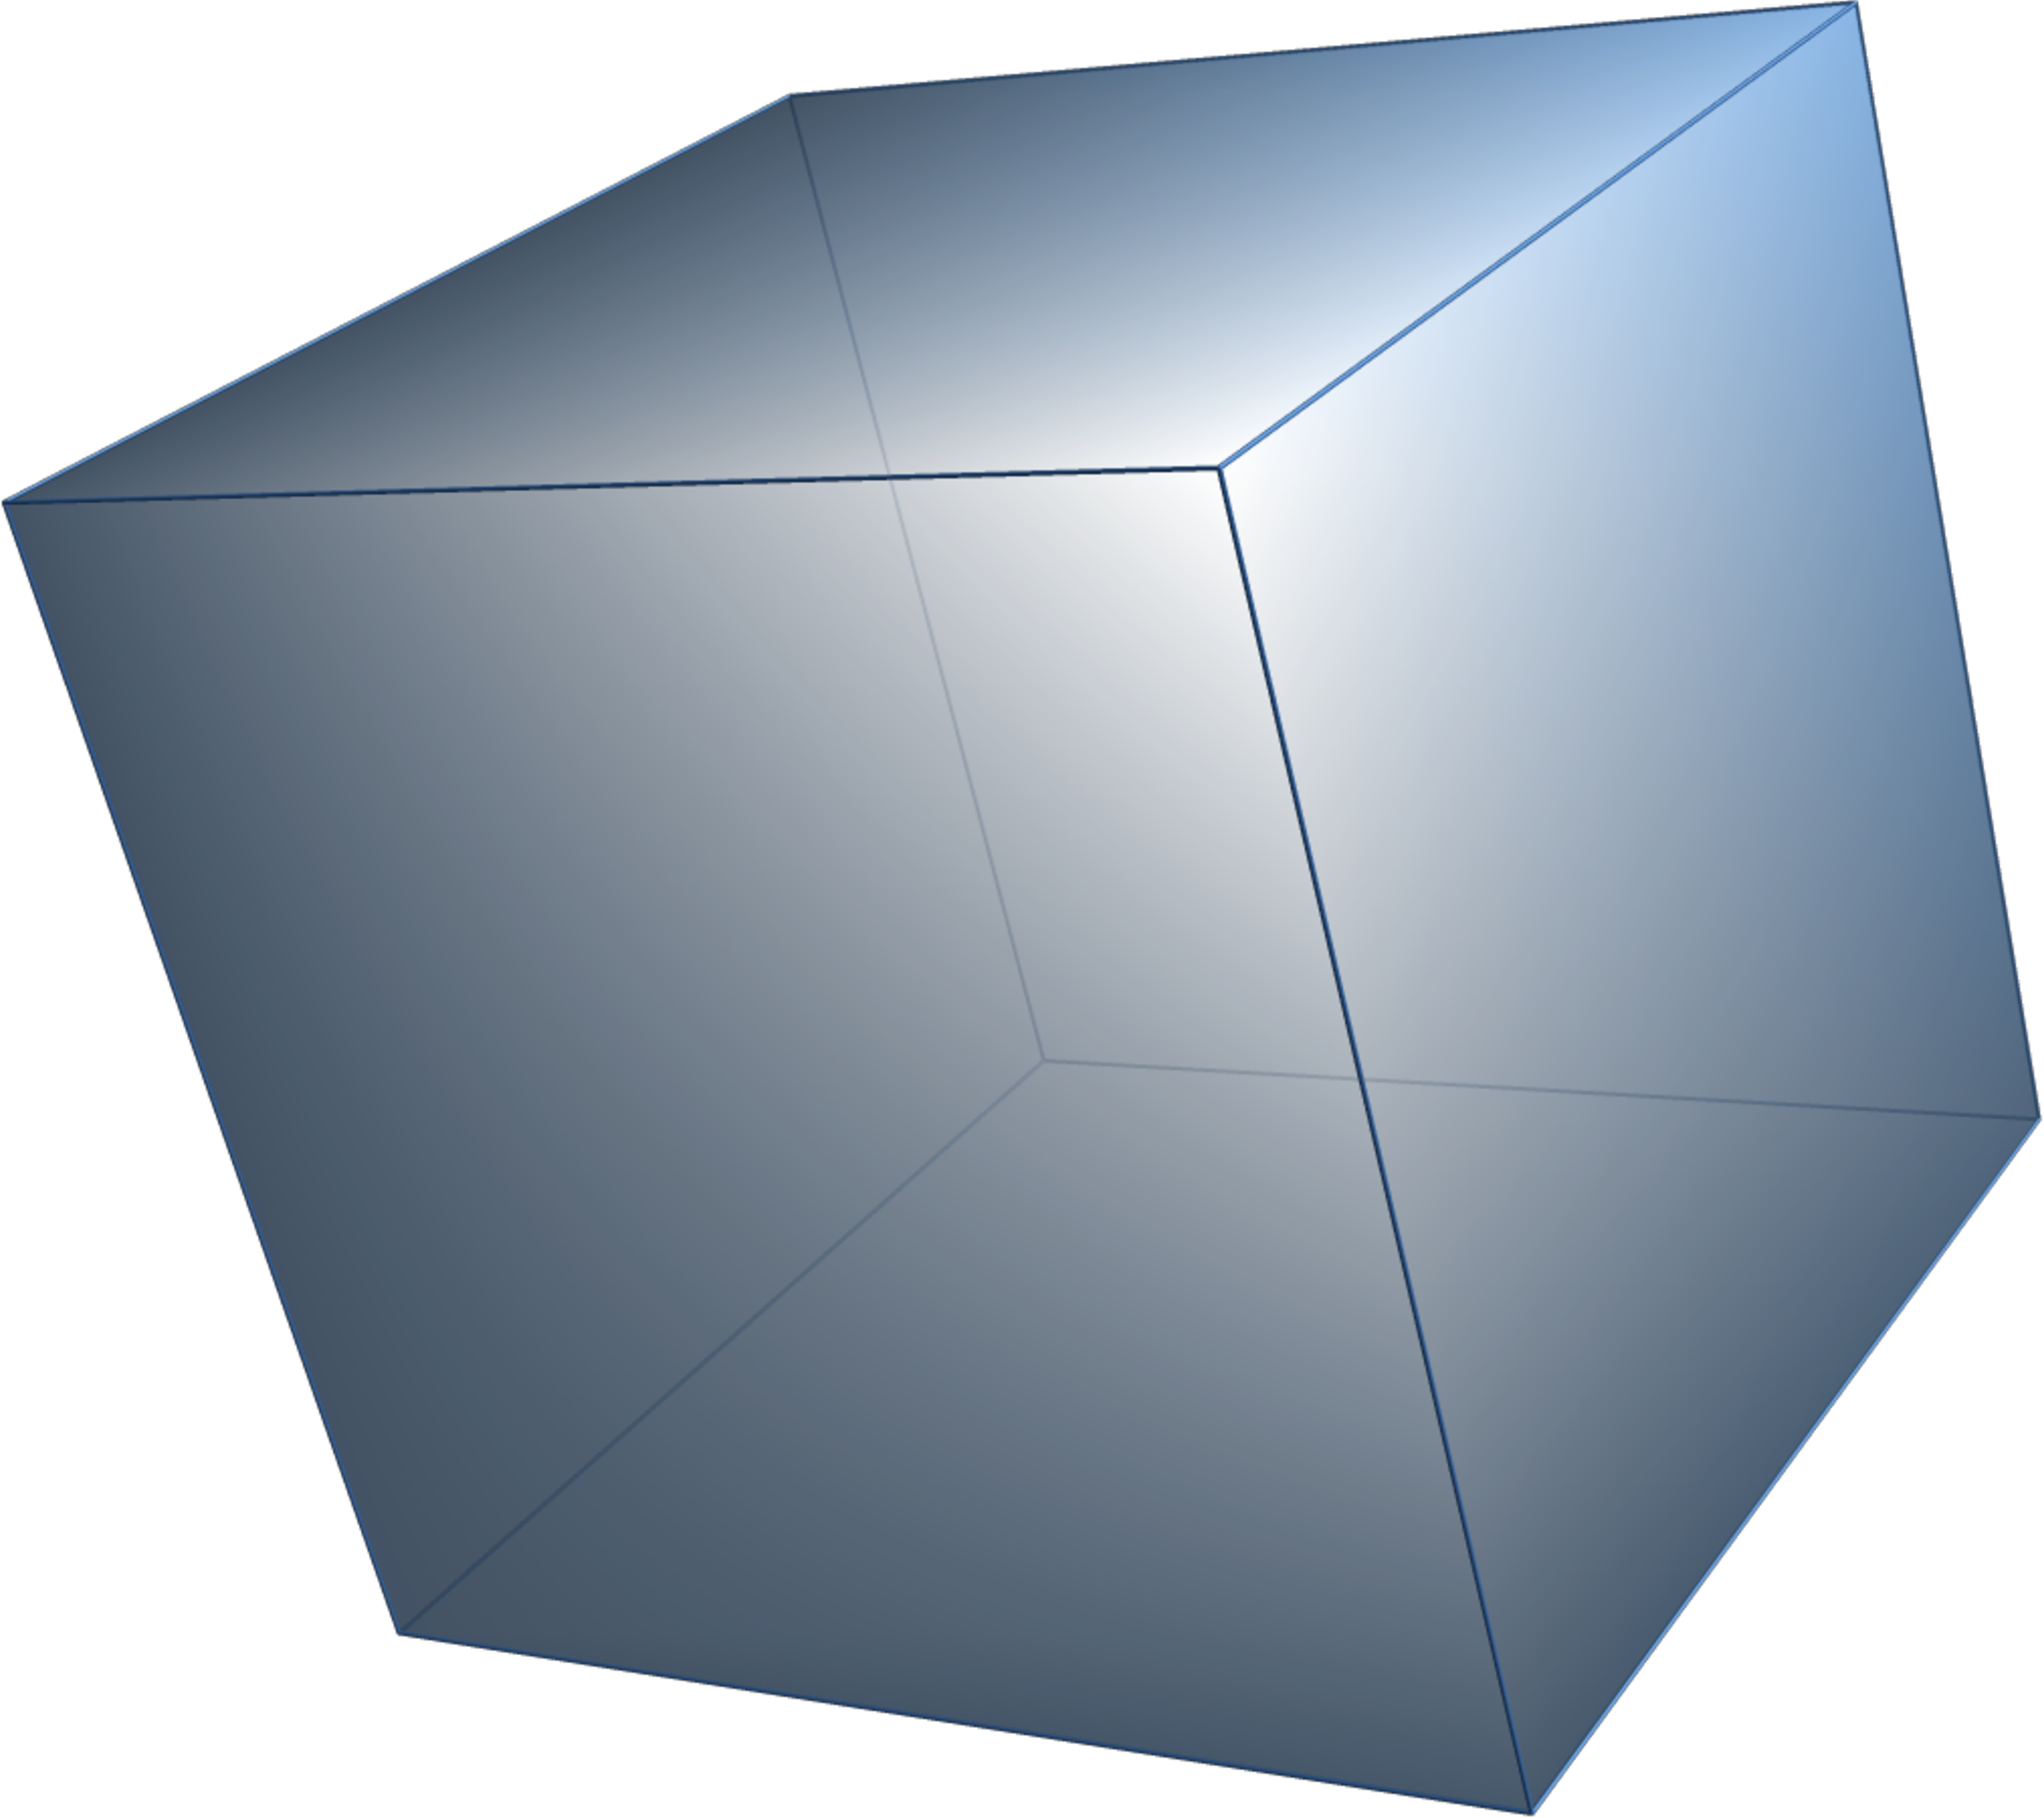
\includegraphics[align=t,width=\linewidth]{cube.pdf}
\\[\jot]%
{\footnotesize\color{mpcolor}\enquote{How much energy is there in this volume at this instant?} This question cannot be answered until we have specified which coordinate system we're using.\par}
}
This is an important difference between energy on one side, and matter and electric charge on the other side. \emph{For matter and electric charge, the questions above can be answered unambiguously independently of any coordinate system}. But not so for energy. The reason of this quirky difference is ultimately connected with the fact that time and space are also observer-dependent.

This coordinate-dependence is not a problem: we must always specify our coordinate system anyway, in order to agree on the time and position of physical events. But it can cause problems when we calculate \emph{changes} in energy. If we first calculate or measure some amount of energy in a coordinate system, then we calculate or measure another amount at some later time in a \emph{different} coordinate system, the difference between the two amounts has no meaning whatsoever. In fact it could happen that there's no energy change at all in one coordinate system or in the other: any change we found was just an artefact of mixing up coordinates.

\begin{warning}[Amounts of \energym\ are coordinate-dependent]
  Never change coordinate system in the middle of energy calculations!
\end{warning}

\medskip

Also the distinction among different forms of energy is coordinate-dependent. For instance, in one coordinate system we can say that a given volume contains only internal energy; but in another coordinate system that same volume can be said to contain internal and kinetic energy.

\marginpar{%
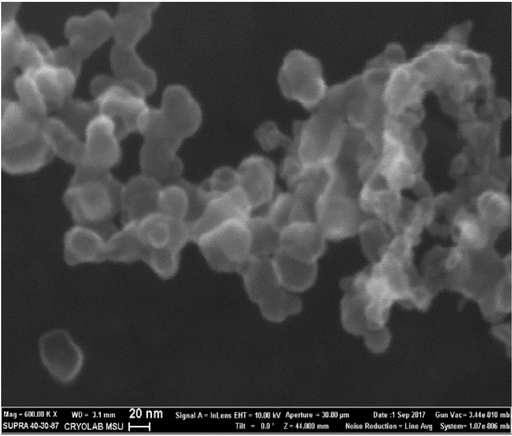
\includegraphics[align=t,width=\linewidth]{molecules_20nmb.png}
\\[\jot]%
\footnotesize{\color{mpcolor}\furl{https://doi.org/10.4209/aaqr.2019.04.0177}{Hydrocarbon fuel particles}. The small blobs have size of around \qty{2e-8}{m}.}
}
The distinction among different forms of energy also depends on the observation scale and on the theory used. For instance, we can observe and model the gas in a container on a scale of metres, seeing it as a uniform flux; in this case we say that there's internal energy in the container. But if we observe and model the gas as a collection of molecules, on a microscopic scale, then we say that there's internal energy (of the single molecules) and kinetic energy in the container (the total energy being the same, unless we have changed coordinate system).

The same is true of energy flux: what we call \enquote*{heat} on one observation scale is \enquote*{work} on a finer scale. % In phenomena that involve matter and electromagnetic fields, any separation between \enquote*{energy of matter} and \enquote*{energy of electromagnetic field} is often arbitrary.

% \begin{warning}[Amounts of \energym\ are coordinate-dependent]
%   Never change coordinate system in the middle of a calculation of energy change!
%   Although the distinction of energy forms is often useful, it's important to keep in mind that it is not absolute: \emph{it depends on the coordinate system, on the scale of observation, and on the theory used}.
% \end{warning}

% So whenever you hear about a distinction between forms of energy or energy fluxes, pay attentionwhich coordinate system and which observation scale are being used.

% Energy-mass is present wherever there's matter, charge, or magnetic flux, and vice versa. \emph{Its specific relation with these quantities depends on the coordinate system} (\sect\,\ref{sec:coords}) that we choose. It is extremely important to keep in mind this dependence. For instance, in the examples above we said that the unstretched rubber band in motion had a \masse\ of \qty{0.000500000000000002}{kg}; but if we choose a coordinate system in which the band is not moving, its \masse\ would be \qty{0.000500000000000000}{kg}. Owing to this coordinate dependence, and depending on whether matter or magnetic flux is present in a region, we often conveniently partition an amount of energy into different \enquote{forms} such as rest energy, internal energy, kinetic energy, gravitational potential energy, electromagnetic energy. This is only a conceptual division.
% 
% Also energy flux can be partitioned depending on the coordinate system and on whether there's also a flux of matter. This leads to the important distinction between two forms of energy flux: \textbf{heat} and \textbf{work}.
% 
% We shall see later how to define and calculate these different forms of energy and energy flux.

\smallskip

\begin{definition}{Energy-mass: notation}
  The amount of energy in a region is usually denoted with $\yE$, or with $\yM$ if we describe it as mass. Internal energy is denoted $\yU$, kinetic energy $\yEk$, potential energy $\yEp$.

  \smallskip
  
  The total flux of energy will be denoted by $\yH$; the flux in the form of heat, by $\yQ$; and in the form of work, by $\yW$.
\end{definition}


\medskip

\begin{exercise}
  In an hour, 14 people exit through a door. Taking the average human weight to be \qty{62}{kg} \parencites{walpoleetal2012}, what's the average \emph{energy} flux, in \unit{J/s}, through that door?
\end{exercise}



% *** we shall see later in \sect

% electron: 8.2e-14 J
% 1e4 J intake
% 1 cal = 4 J
% 1 kg = 9e16 J
% U = 50/2*0.1^2 = 0.25 J = 3e-18 kg

\section{Momentum}
\label{sec:intro_momentum}

Momentum, also called \emph{linear momentum} or \emph{translational momentum} to distinguish it from angular momentum, is a \emph{vector} quantity. Its SI dimension and units can be written in several equivalent ways; we shall keep in mind especially these three:
\begin{equation*}
  \begin{gathered}
    \textsf{force}\times\textsf{time}
    \\\unit{N\cdot s}
  \end{gathered}
\enspace  \equiv\enspace
  \begin{gathered}
  \textsf{mass}\times\textsf{length}/\textsf{time}
    \\\unit{kg\cdot m/s}
  \end{gathered}
\enspace  \equiv\enspace
  \begin{gathered}
  \textsf{energy}\times\textsf{time}/\textsf{length}
    \\\unit{J\cdot s/m}
  \end{gathered}
\end{equation*}
% $\textsf{energy}\times\textsf{time}/\textsf{length}$, and accordingly measured in units of $\emph{joules}\times\emph{seconds}/\emph{metres}$ (\unit{J\cdot s/m}), or equivalently with SI dimension $\textsf{mass}\times\textsf{length}/\textsf{time}$, and accordingly measured in units of $\emph{kilograms}\times\emph{metres}/\emph{seconds}$ (\unit{kg\cdot m/s}). 
Since it is a vector quantity, it is usually expressed with three numbers, typically the $x$-, $y$-, and $z$-components. In simplified problems where only one or two dimensions are relevant, only the relevant components are reported.
% \mynotew{use \unit{N\cdot s}}

Momentum is a subtle quantity, even subtler than energy. Textbooks that focus on Newtonian mechanics \emph{define} it as the product of the mass and the velocity of a body, usually written \enquote{$\bm{p}=m\bm{v}$}. This relation, however, is only valid in special circumstances, and cannot be used in many everyday technological applications, especially when electromagnetism is involved. And that relation is actually only an approximation even in the circumstances where it's used.

% First, it is true that where there's matter in motion there's also momentum; but this momentum is given by \enquote*{mass${}\times{}$velocity} only as an approximation. Second, there can be momentum also where there is no matter; for instance where there is magnetic flux. If you prepare a sealed glass box which is completely empty of matter within (you create a vacuum), there still is momentum within the box if light or electromagnetic waves are present. We shall discuss later some technological uses of this fact.

It is therefore convenient to separate our idea of momentum from the idea of \enquote{objects} moving, keeping in mind that the latter idea is just a particular case of momentum. Yet, \emph{momentum is indeed associated with translational motion} of matter and of electromagnetic fields. \emph{Translational} motion is the kind of motion that leads to a \emph{new position} in space. For instance, when you walk from one place to a different one, you have performed translational motion (note that translational motion doesn't need to be in a straight line).% We shall moreover see that there is an important connection between momentum and our intuitive idea of \enquote*{force}.

Just as energy is often mentally visualized as a sort of fluid (although this visualization comes with many warnings), also momentum can actually be visualized as a sort fluid; but you must imagine it as a \enquote{fluid of vectors}.
\marginpar{%
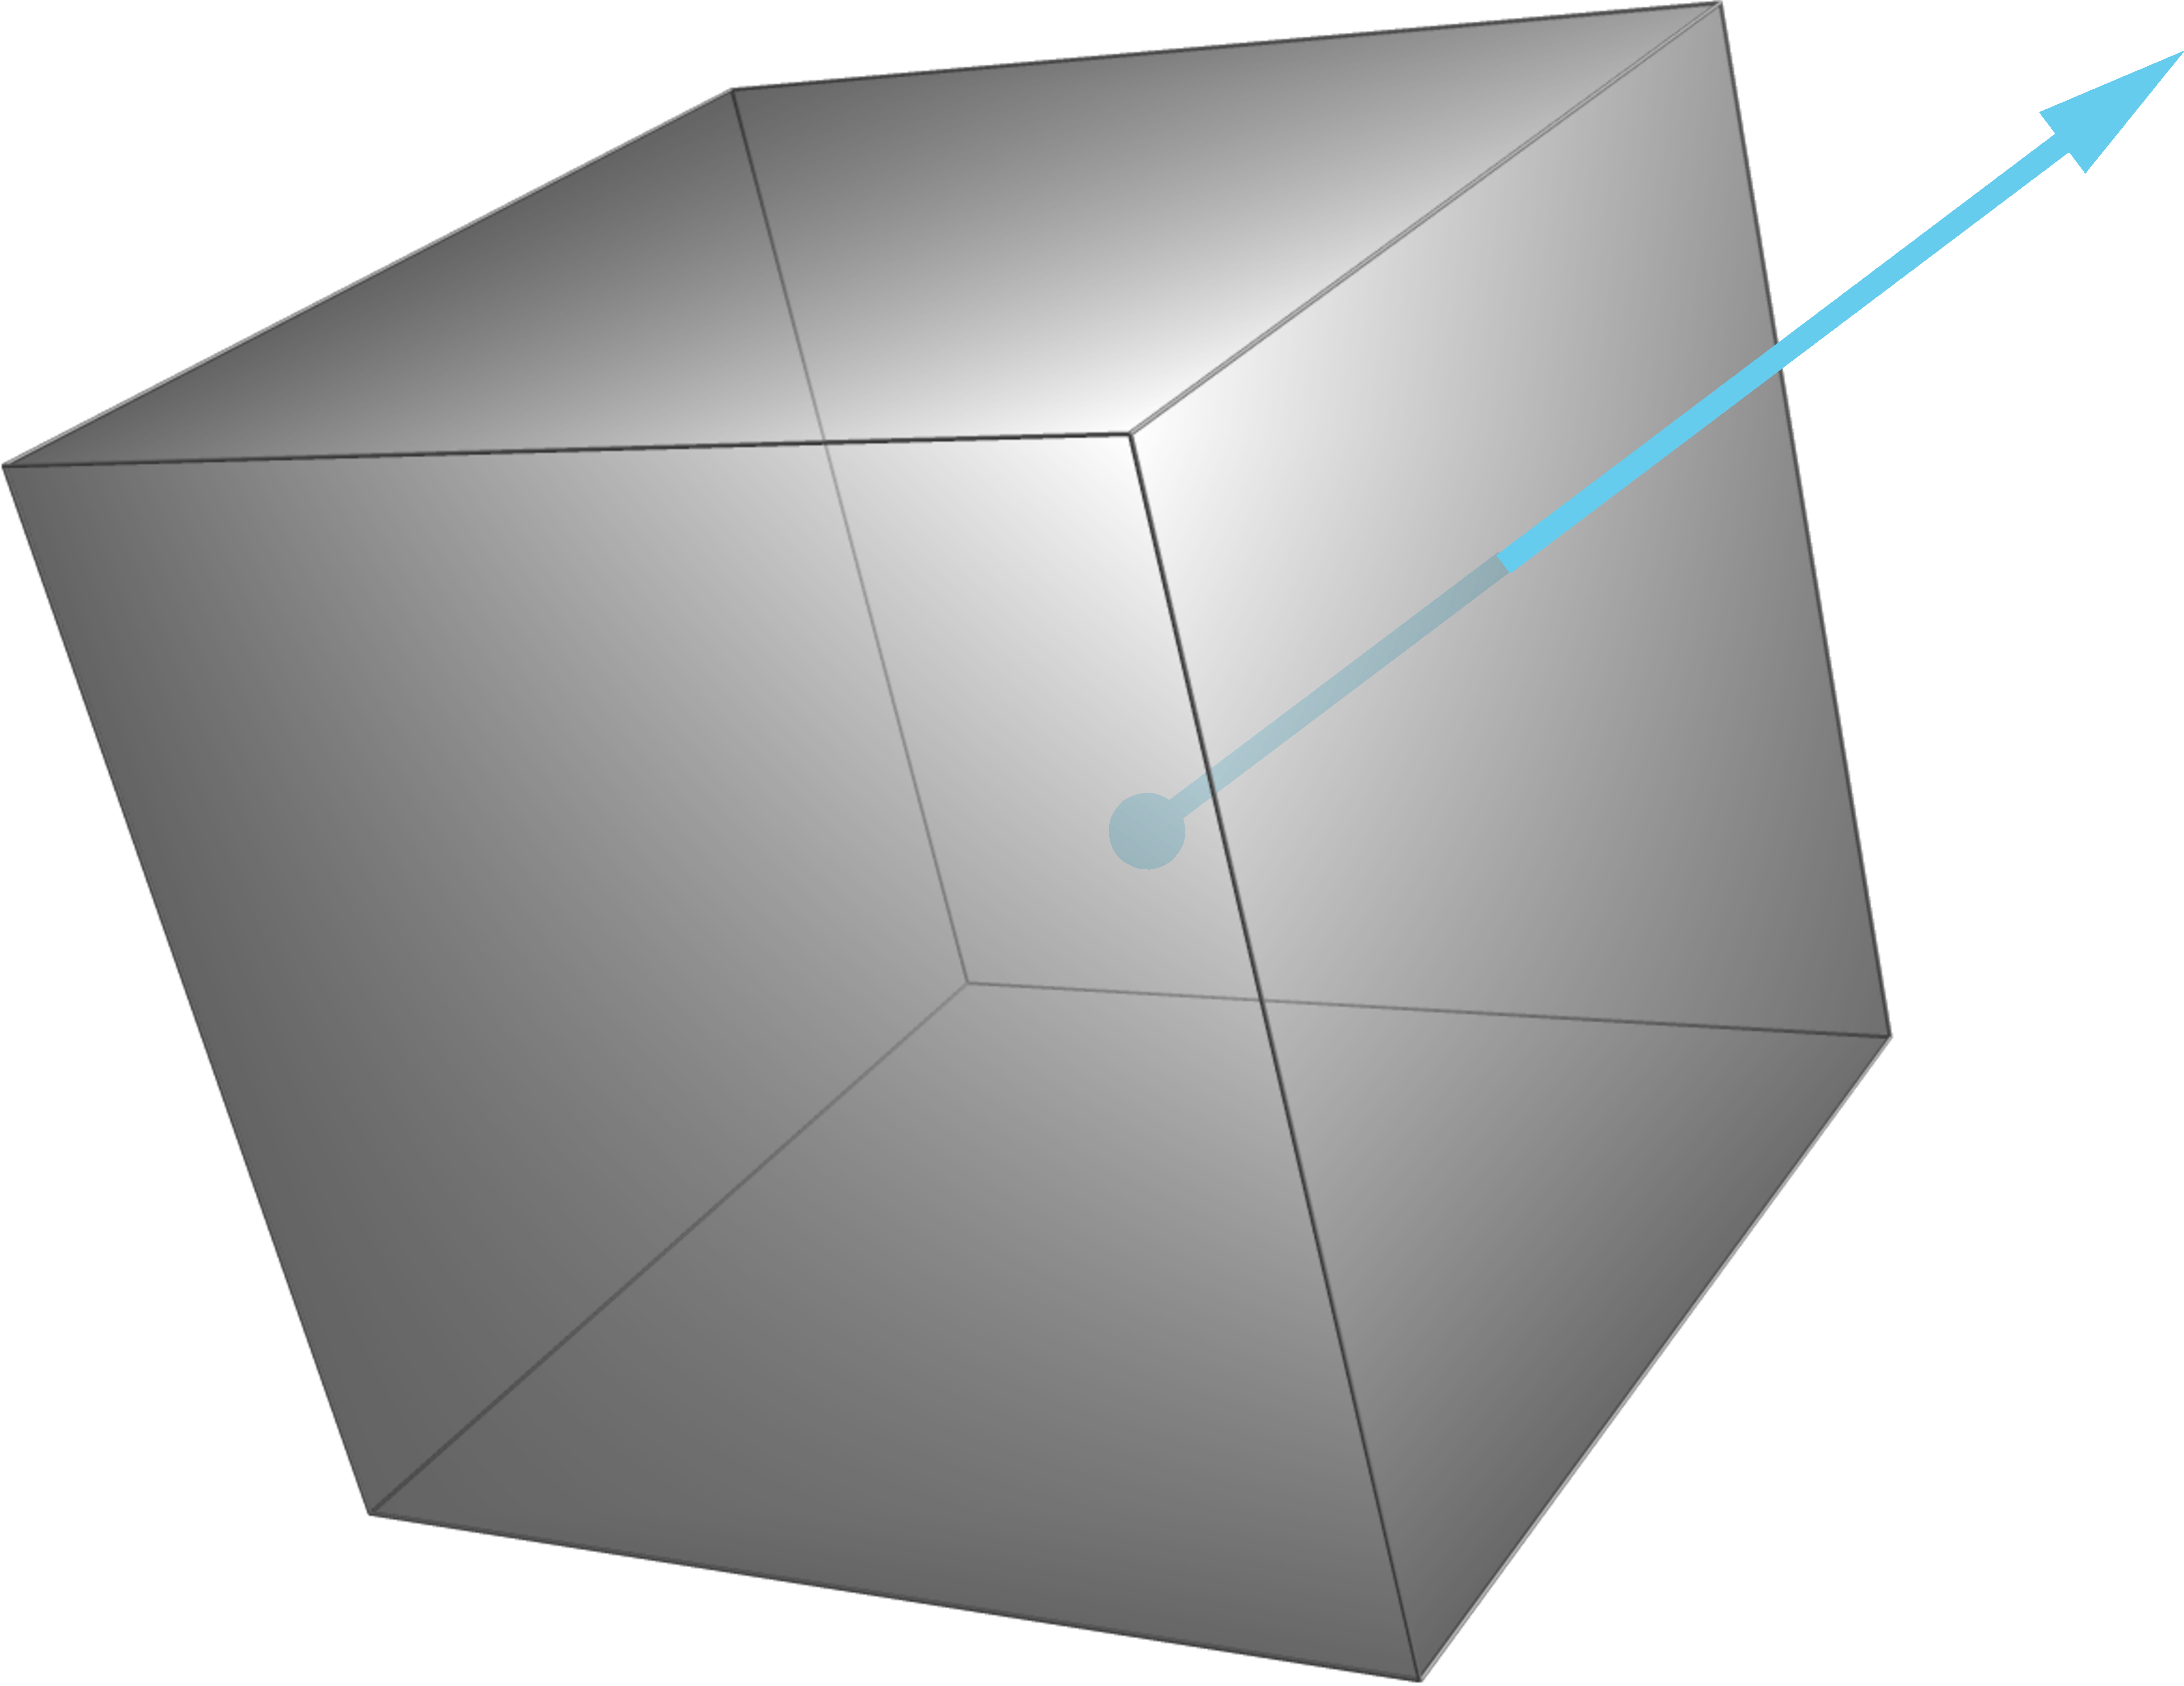
\includegraphics[align=t,width=\linewidth]{cubearrow.pdf}
\\[\jot]%
\footnotesize{\color{mpcolor}The amount of momentum within a volume is represented by a \textcolor{cyan}{(3D) vector}}
}
Given a particular volume at a particular instant in time, and given a coordinate system, we can speak of the total amount of momentum within that volume. This amount is represented by a \emph{vector}. You can imagine a continuous collection of vectors filling the volume, possibly with different directions and small magnitudes; the total momentum is the sum of all these vectors. This visualization obviously comes with many warnings, but it can be very useful if we are careful.

And just as energy, the total amount of momentum is \emph{coordinate-dependent}. So we have the same warning here:
\begin{warning}[Amounts of momentum are coordinate-dependent]
  Don't change coordinate system in the middle of calculations of momentum!
\end{warning}


Flux of momentum is what we call \textbf{force}. A static force, like the one you exert when you hold a bag, is often mentally visualized as a static vector. In \chap\,\ref{cha:total_flux} we shall discuss a different visualization, in which force is represented as a sort of flow of vectors.

% Force is a notion that we understand intuitively and that we can \enquote{feel} with our own bodies. In Newtonian mechanics it's often taken as primitive, and is represented by a vector. But it can also be defined and interpreted as a \emph{flux of momentum}. This point of view can be very useful and even more intuitive in some situations. We shall discuss it more in depth in \sect\,\mynotew{}.


\begin{definition}{Momentum: notation}
  The amount of momentum in a region is usually denoted with $\yP$. The flux of momentum is also called force and denoted with $\yF$.
\end{definition}



\begin{extra}{Momentum and energy flux are the same}
  According to Relativity Theory, momentum \emph{is} energy flux (such as heat), and energy flux \emph{is} momentum. If we represent momentum with the symbol $\bm{P}$, and energy flux with the symbol $\bm{Q}$, the equivalence between them is given by
  \begin{equation}
    \label{eq:momentum_heat}
    \bm{Q} = \bm{P}c^{2}
  \end{equation}
  Compare this formula with $E=mc^{2}$. From this point of view, you can think of momentum as \enquote{energy in motion}. This is consistent with our discussion about \masse: since mass is energy, the Newtonian expression \enquote{$m\bm{v}$} indicates energy in motion, or a flux of energy. On a sunny day, if you close your eyes and feel the Sun's heat on your face, what you are feeling is actually a flow of momentum. And when you kick a ball, you're setting a huge bundle of energy in motion, and that's why the ball has acquired momentum.
\end{extra}



\section{Angular momentum}
\label{sec:intro_angmomentum}

Angular momentum, also called \emph{moment of momentum} or \emph{rotational momentum}, is a \emph{vector} quantity. Its SI dimension and units can be written in several equivalent ways; we shall keep in mind especially these three:
\begin{equation*}
  \begin{gathered}
    \textsf{force}\times\textsf{length}\times\textsf{time}
    \\\unit{N\cdot m\cdot s}
  \end{gathered}
\enspace  \equiv\enspace
  \begin{gathered}
  \textsf{mass}\times\textsf{length}^{2}/\textsf{time}
    \\\unit{kg\cdot m^{2}/s}
  \end{gathered}
\enspace  \equiv\enspace
  \begin{gathered}
  \textsf{energy}\times\textsf{time}
    \\\unit{J\cdot s}
  \end{gathered}
\end{equation*}
% , with SI dimension $\textsf{energy}\times\textsf{time}$, and accordingly measured in units of $\emph{joules}\times\emph{seconds}$ (\unit{J\cdot s}), or equivalently with SI dimension $\textsf{mass}\times\textsf{length}^{2}/\textsf{time}$, and accordingly measured in units of $\emph{kilograms}\times\emph{metres}^{2}/\emph{seconds}$ (\unit{kg\cdot m^2/s}).
It is usually expressed with three numbers, typically the $x$-, $y$-, and $z$-components.

Angular momentum is probably an even subtler quantity than momentum. Just as momentum is associated with translational motion, angular momentum is associated with \emph{rotational} motion. Rotational motion is the kind of motion that leads to a \emph{new orientation} in space, rather than to a new position. For instance, if you turn to your left or to your right while standing in place, you have performed rotational motion.

There isn't a clear-cut distinction between translational and rotational motion: usually they involve each other to some degree. A translational motion can be interpreted as a rotation around a point that is very far away; and a rotation of an extended object can be interpreted as small translational motions of its parts.

This is the reason why in many situations we can calculate angular momentum in terms of momentum. % so even if we don't fully grasp it intuitively, we can still calculate it
If the momentum in a \emph{small} volume is denoted by the vector $\yP=(P_{x},P_{y},P_{z})$, and the position vector by $\yr=(x,y,z)$, then the angular momentum $\yL=(L_{x}, L_{y}, L_{z})$ \emph{with respect to the origin of coordinates}, in that same volume, is given by the vector product
\begin{subequations}
  \begin{equation}
    \label{eq:ang_momentum_def}
    \begin{gathered}
      \yL = \yr \times \yP
      \\
      \text{or equivalently}\qquad\left\{\enspace
        \begin{aligned}
          L_{x} & = y\,P_{z} - z\,P_{y}
          \\    L_{y} & = z\,P_{x} - x\,P_{z}
          \\    L_{z} & = x\,P_{y} - y\,P_{x}
        \end{aligned}\right.
    \end{gathered}
  \end{equation}
  Instead of calling the components \enquote{$(L_{x}, L_{y}, L_{z})$}, we can also call them \enquote{$(L_{yz}, L_{zx}, L_{xy})$}, as some books do. The latter names make the formulae above easier to remember:
  \begin{equation}
    \label{eq:ang_momentum_def_bis}
\left\{\enspace
    \begin{aligned}
      L_{yz} & = y\,P_{z} - z\,P_{y}
      \\    L_{zx} & = z\,P_{x} - x\,P_{z}
      \\    L_{xy} & = x\,P_{y} - y\,P_{x}
    \end{aligned}\right.
\end{equation}
\end{subequations}
Choose whichever you prefer.

Angular momentum is something that is associated not only with ordinary bodies (matter), but also with electromagnetic fields. Just like momentum, also angular momentum can be visualized as a \enquote{fluid of vectors}.
%
\marginpar{%
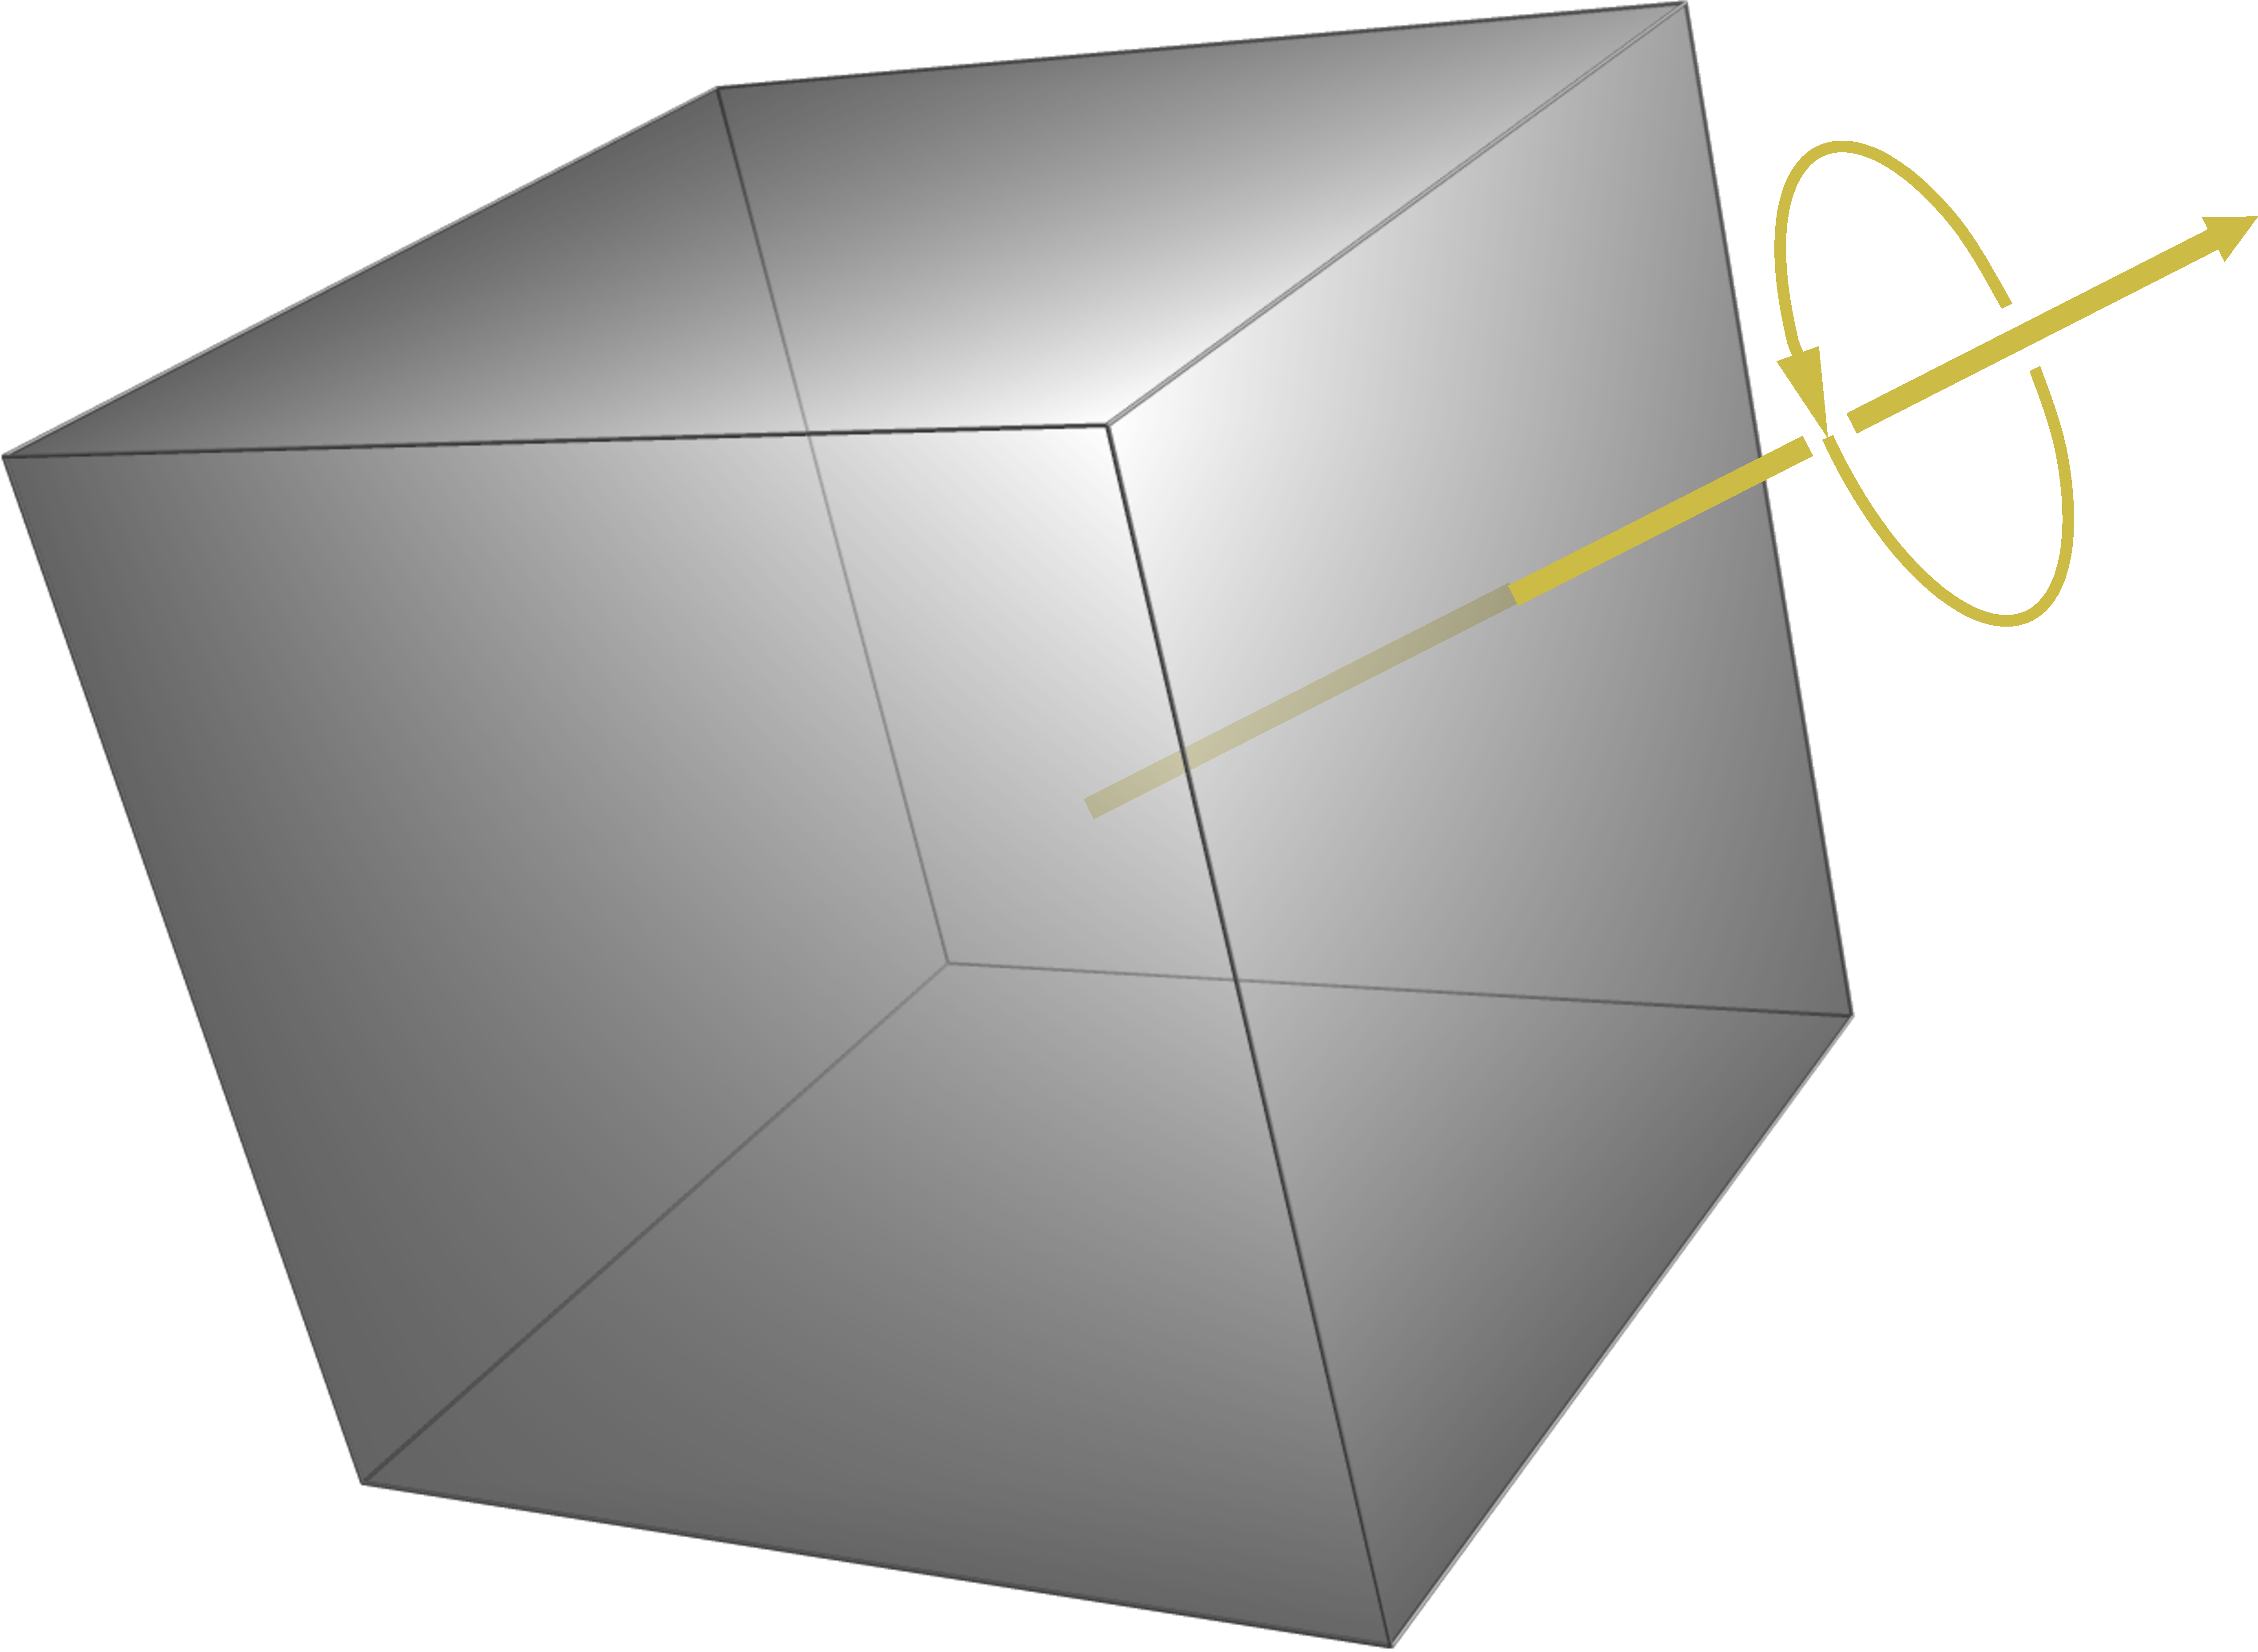
\includegraphics[align=t,width=\linewidth]{cubetwistedarrow.pdf}\label{fig:volumetwistedarrow}%
\\[\jot]%
\footnotesize{\color{mpcolor}The amount of angular momentum within a volume is represented by a \textcolor{yellow}{(3D) vector}. (Curious about the little circulation symbol around the vector? Then read on.)}
}
Given a particular volume at a particular instant in time, and given a coordinate system, we can speak of the total amount of angular momentum within that volume. This amount is represented by a \emph{vector}, and is \emph{coordinate-dependent}:
\begin{warning}[Amounts of angular momentum are coordinate-dependent]
  Don't change coordinate system in the middle of calculations of angular momentum!
\end{warning}

\smallskip

The flux of angular momentum is also called the \emph{torque}, and bears a relation to the flux of momentum similar to the formula above. If the force -- flux of momentum -- is denoted by the vector $\yF=(F_{x},F_{y},F_{z})$ and the position vector by $\yr=(x,y,z)$, then the flux of angular momentum, or torque, $\yT=(\tau_{x}, \tau_{y}, \tau_{z})$ \emph{with respect to the origin of coordinates} is given by
  \begin{equation}
    \label{eq:torque_def}
    \begin{gathered}
      \yT = \yr \times \yF
      \\[\jot]
      \text{or equivalently}\qquad\left\{\enspace
        \begin{aligned}
          \tau_{x} & = y\,F_{z} - z\,F_{y}
          \\    \tau_{y} & = z\,F_{x} - x\,F_{z}
          \\    \tau_{z} & = x\,F_{y} - y\,F_{x}
        \end{aligned}\right.
      \qquad\text{or}\qquad
      \left\{\enspace
    \begin{aligned}
      \tau_{yz} & = y\,F_{z} - z\,F_{y}
      \\    \tau_{zx} & = z\,F_{x} - x\,F_{z}
      \\    \tau_{xy} & = x\,F_{y} - y\,F_{x}
    \end{aligned}\right.
    \end{gathered}
  \end{equation}

  \bigskip

You may wonder:
\enquote{Do we really need angular momentum? after all it just looks like something constructed from momentum}.
% \begin{marginfigure}\footnotesize%
%   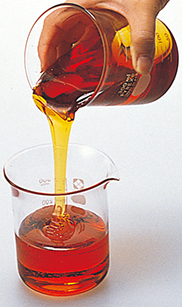
\includegraphics[align=b,width=\linewidth]{polymer.png}
% \\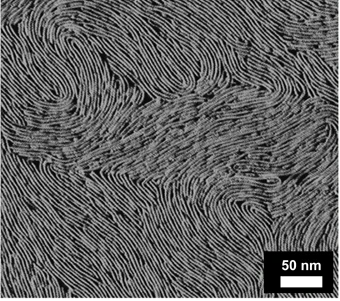
\includegraphics[align=c,width=\linewidth]{polymer2.png} \\[\jot]%
% {\color{green}Some liquid polymers (\textbf{top:} Liquid Diethoxymethane Polysulfide) need to be described with a special kind of angular momentum, owing to their molecular structure (\textbf{bottom}).}
% \end{marginfigure}
\marginpar{\centering%
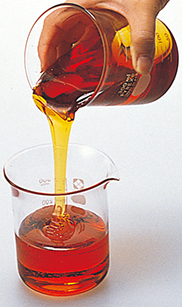
\includegraphics[align=b,width=0.67\linewidth]{polymer.png}
\\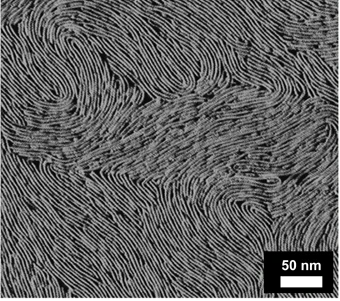
\includegraphics[align=c,width=\linewidth]{polymer2.png}
\\[\jot]\flushleftright%
\footnotesize{\color{mpcolor}Some liquid polymers (\textbf{top:} Liquid Diethoxymethane Polysulfide) need to be described with a special kind of angular momentum, owing to their molecular structure (\textbf{bottom}).}
}%
The answer is yes, we really need it, for two reasons. First, angular momentum obeys an important universal law which is independent from those obeyed by energy and by momentum (\cites{truesdell1963b_r1968} tells some of the story of how this was discovered). % \mynotew{rephrase this}
Second, for some physical phenomena, for example involving liquid \furl{https://www.britannica.com/science/polymer}{polymers},
% https://www.britannica.com/science/polymer
elementary particles, or electromagnetic radiation, the angular momentum includes an additional part, called \emph{spin} or \emph{intrinsic angular momentum}, that is \emph{not} related to linear momentum. In the present notes we shall not use this more general kind of angular momentum.

\smallskip

\begin{definition}{Angular momentum: notation}
  The amount of angular momentum in a region is usually denoted with $\yL$. The torque or flux of angular momentum is denoted with $\yT$.
\end{definition}



\subsection{Angular momentum as a twisted vector}
\label{sec:twisted_vec}

In order to represent angular momentum we can use a kind of vectors different from the arrow-like ones (called \emph{polar} vectors) with which you are probably familiar. They are called \textbf{twisted vectors}, or also \emph{pseudo}-vectors or \emph{axial} vectors or \emph{outer-oriented} vectors. Twisted vectors represent rotations, and therefore have an orientation, not along them, but \emph{around} them:
\begin{center}
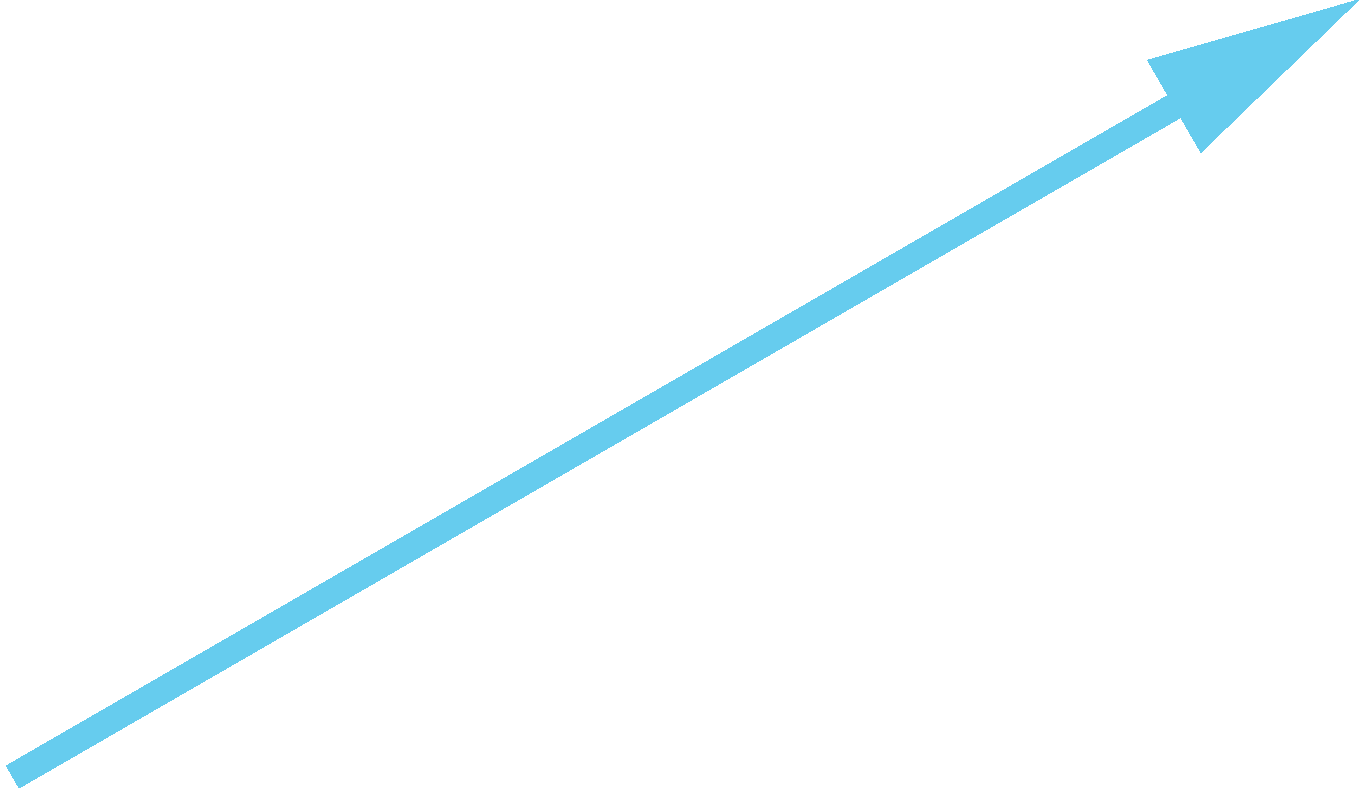
\includegraphics[width=0.34\linewidth]{io-vector.pdf}%
\hspace*{0.12\linewidth}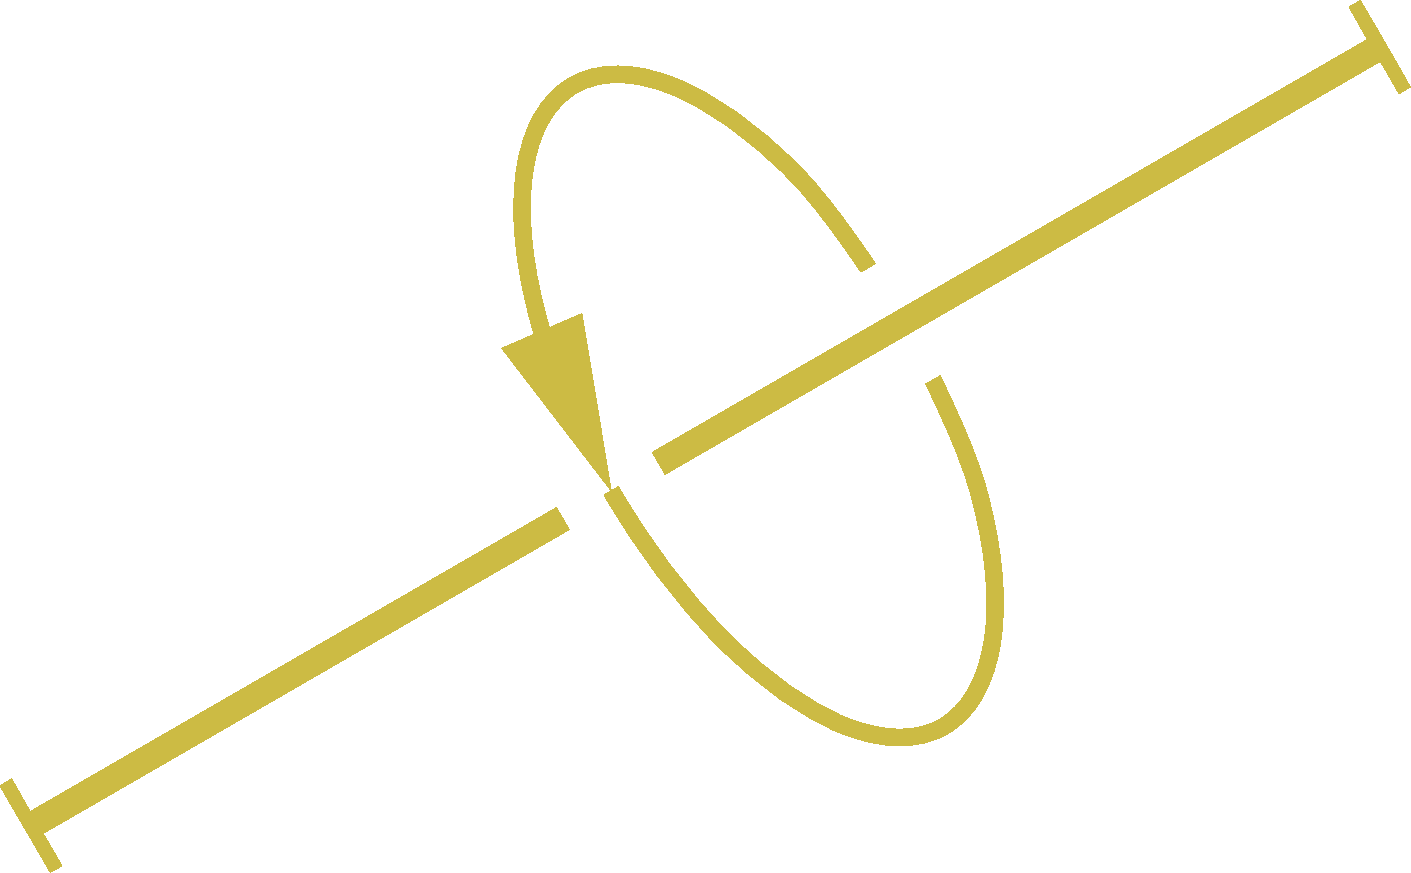
\includegraphics[width=0.34\linewidth]{oo-vector.pdf}%
%
\\\footnotesize
\makebox[0pt][c]{an ordinary vector}\hspace*{0.46\linewidth}\makebox[0pt][c]{a twisted vector}
\end{center}
Their length still represents the magnitude of the vector. They make it immediately clear what is the axis of rotation, and what is the sense of rotation.

The sum of twisted vectors is analogous to the sum of ordinary vectors, with the parallelogram rule:
\begin{center}
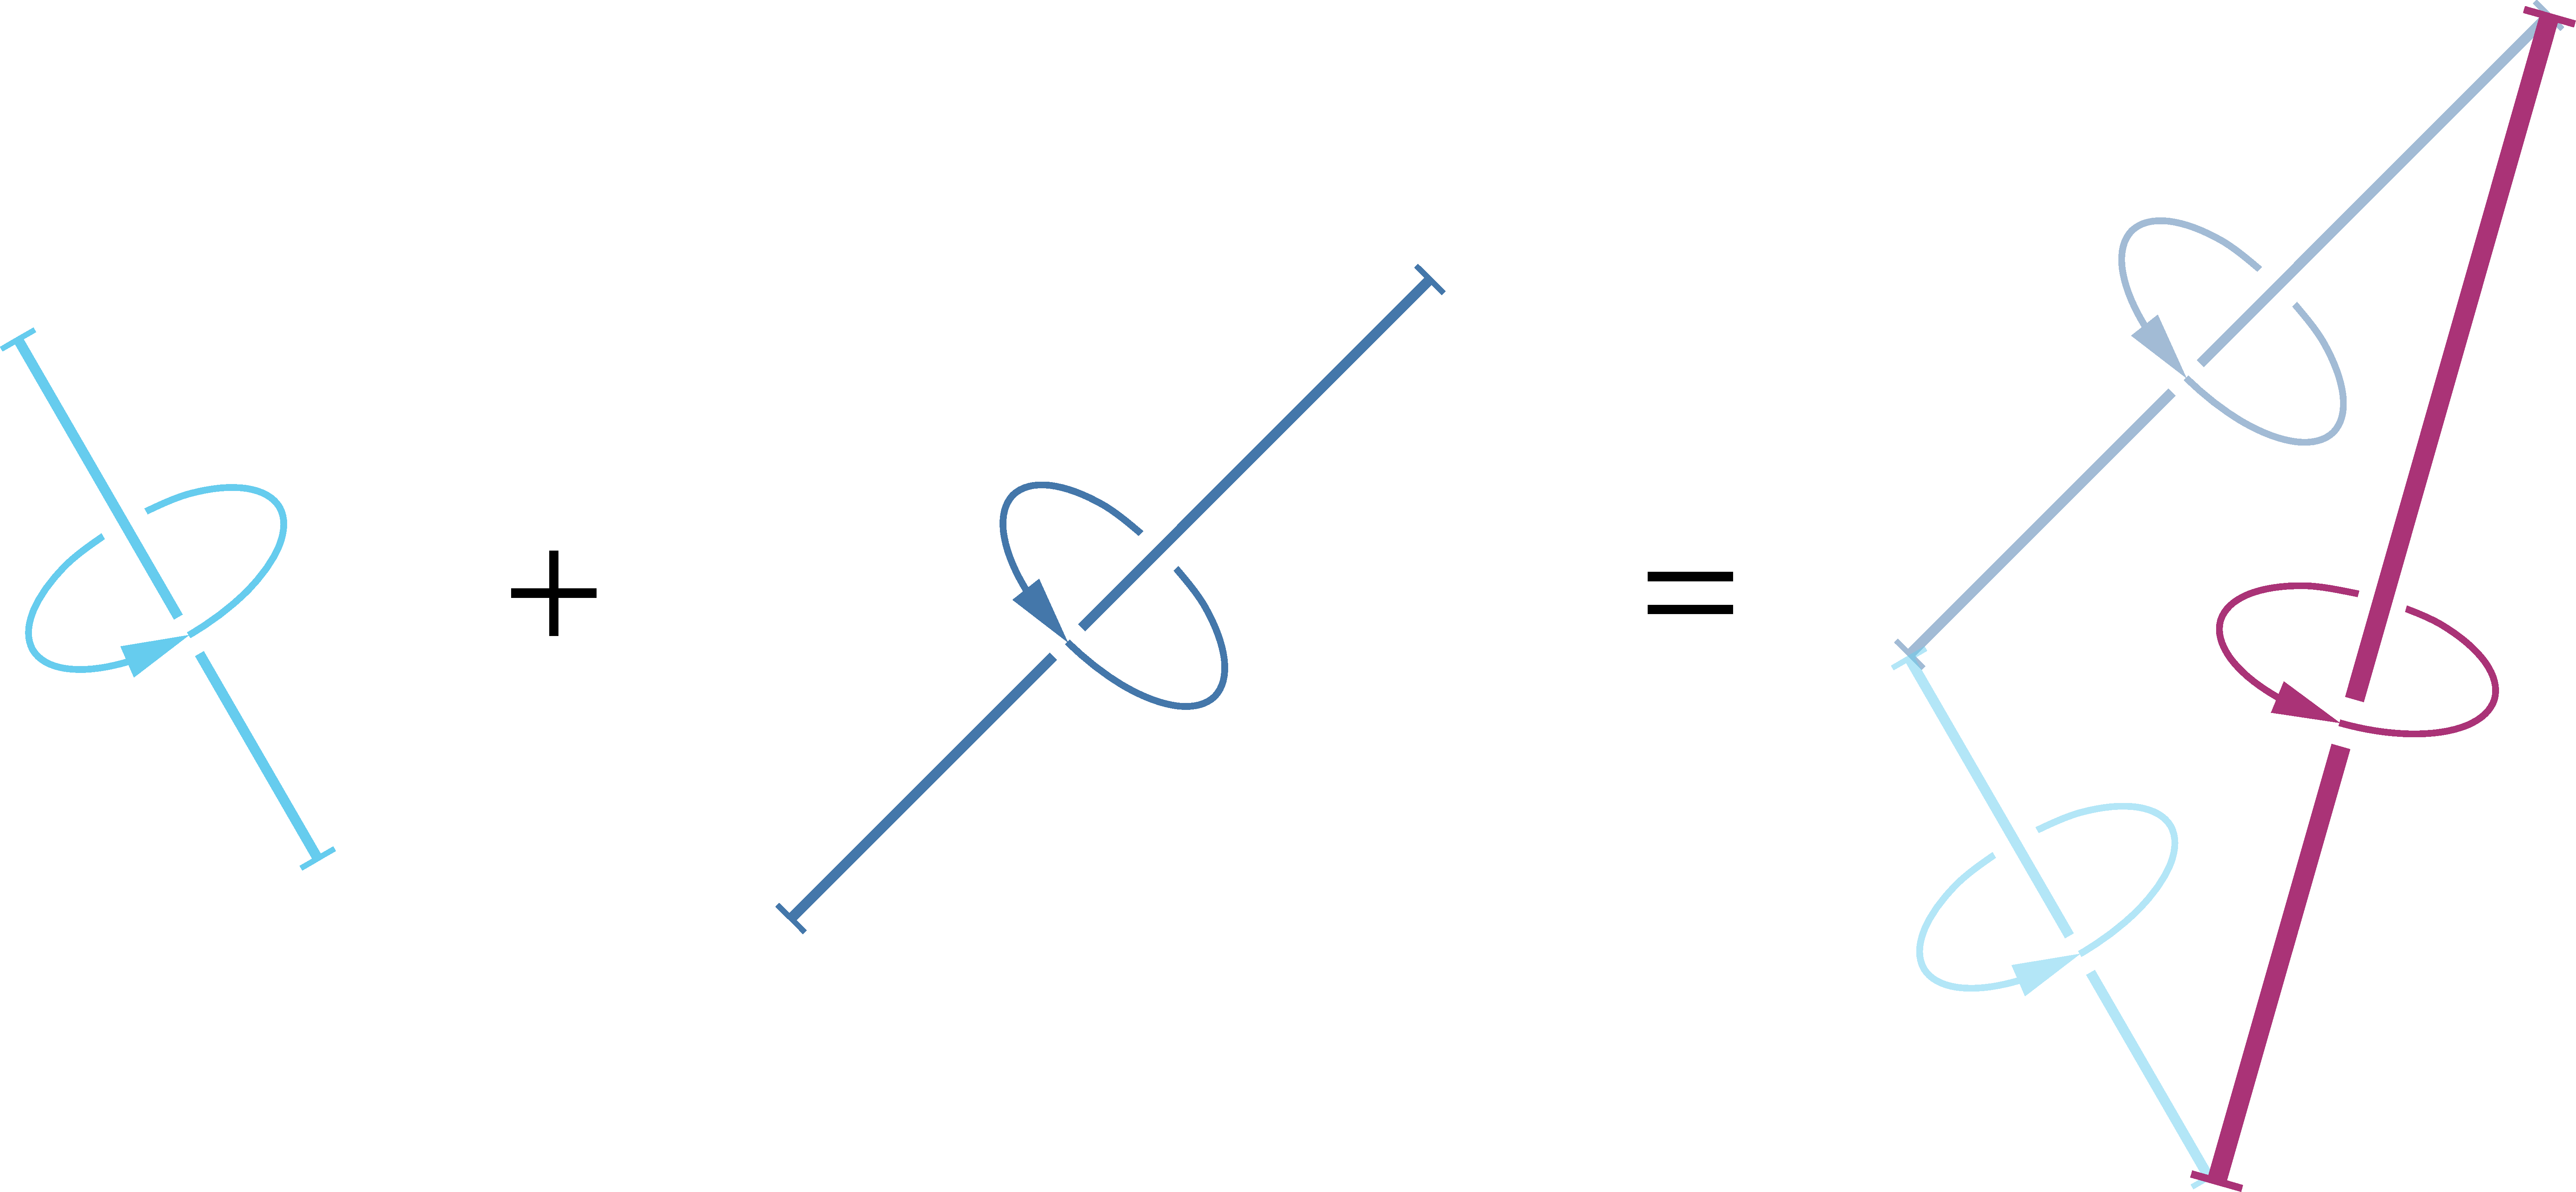
\includegraphics[width=0.67\linewidth]{tvectorsum.pdf}%
\end{center}

Ordinary vectors and twisted vectors behave very differently if we look at their images through a mirror parallel to their axis: the orientation of ordinary vectors appears unchanged, whereas the orientation of twisted vectors appears \emph{reversed}:
\begin{center}
  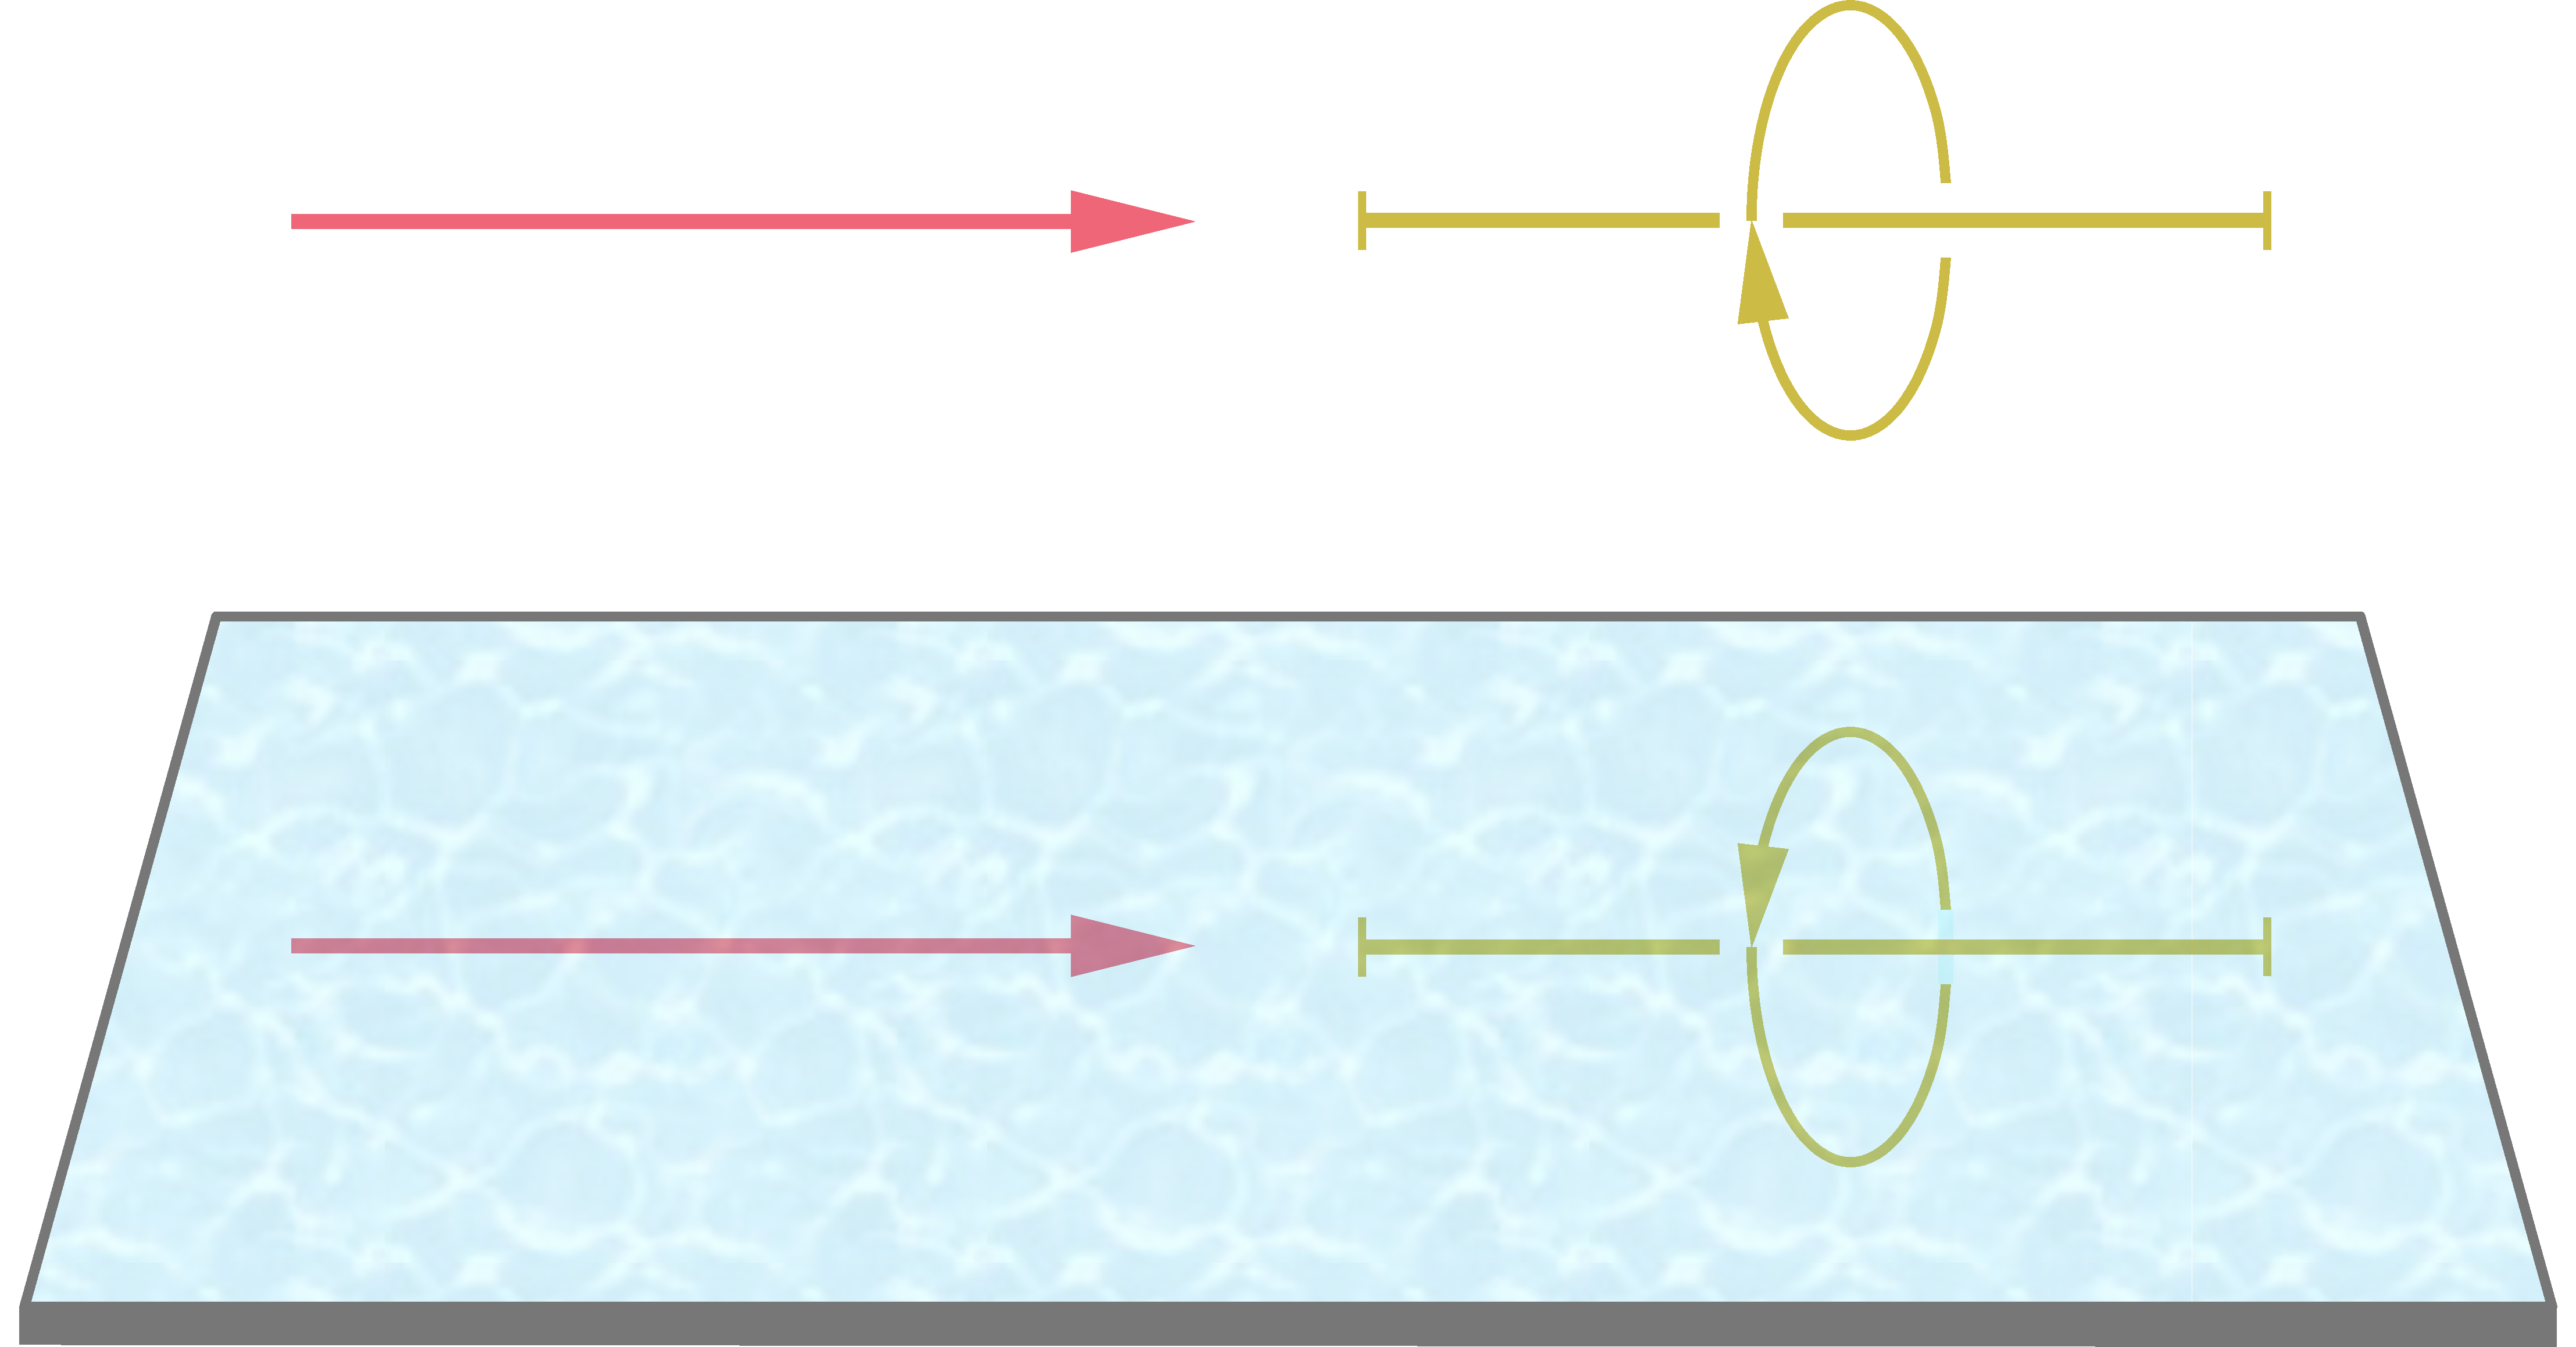
\includegraphics[width=0.67\linewidth]{mirror.pdf}
\end{center}
this phenomenon reflects the behaviour of rotations under reflections.

For some mysterious reason many books are afraid of using twisted vectors, and rely on ordinary vectors instead,
\marginpar{%
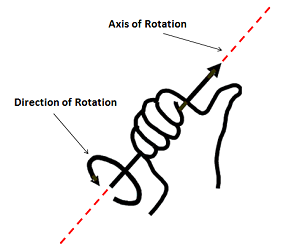
\includegraphics[align=t,width=\linewidth]{curlrighthand.png}
% \\[\jot]%
% \footnotesize{\color{mpcolor}The amount of momentum within a volume is represented by a \textcolor{cyan}{(3D) vector}}
}
introducing the \enquote{right-hand rule} to determine the sense of rotation from the arrow of the ordinary vector. If you've ever asked yourself \enquote{why the right hand, and not the left hand?}, the answer is that it's purely a convention; one could have introduced a left-hand rule instead. Using twisted vectors we don't need these arbitrary conventions and mnemonics: the sense of rotation is unequivocally indicated by the twisted vector.

Use whichever vector representation you prefer. In these notes we shall use a hybrid notation, as in the side picture of p.~\pageref{fig:volumetwistedarrow}, so as to make everybody (or no one) happy.

\begin{exercise}
  A GPS satellite has, at a given instant, the following position and momentum:
  \begin{equation*}
    \begin{split}
      \yr &=\bigl[
      \num[exponent-mode=scientific]{1.4e+7}\,,\ 
      \num[exponent-mode=scientific]{1.6e+7}\,,\ 
      0\bigr]\:\unit{m}
      \\[\jot]
      \yP &=\bigl[
      \num[exponent-mode=scientific]{-3.1e+6}\,,\ 
      \num[exponent-mode=scientific]{3.4e+6}\,,\ 
      0\bigr]\:\unit{N\cdot s}
    \end{split}
  \end{equation*}
  Assuming that the satellite's volume can be considered as small for some purpose, calculate the satellite's angular momentum.
\end{exercise}


\bigskip

\begin{extra}{{What are energy, momentum, angular momentum?}}
From the discussions and formulae above, it seems that \energym, momentum, angular momentum are quite closely related to one another. For all three, the amount in a volume or through a surface is undefined unless we specify a coordinate system. And we shall see later that all three satisfy balance laws but not necessarily conservation laws.

  Relativity Theory indeed shows that energy, momentum, angular momentum are different aspects of one single geometric object, called \emph{energy-momentum tensor}. They are like its \enquote{shadows}, that we can observe by looking at it from different points of view in time and space. This is also why their values get intermixed if we change our system of coordinates. %

  General Relativity gives a new meaning to these quantities: they are \emph{particular curvatures of spacetime}. They express how spacetime is curved in different directions. So whenever we measure, say, the energy or the momentum of some object or of some electromagnetic radiation, we are actually measuring how much that object or radiation is curving spacetime in a particular way. % We shall discuss further connections between these three quantities and spacetime in \sect\,\mynotew{}.
\end{extra}
\marginpar{\vspace{-11em}%
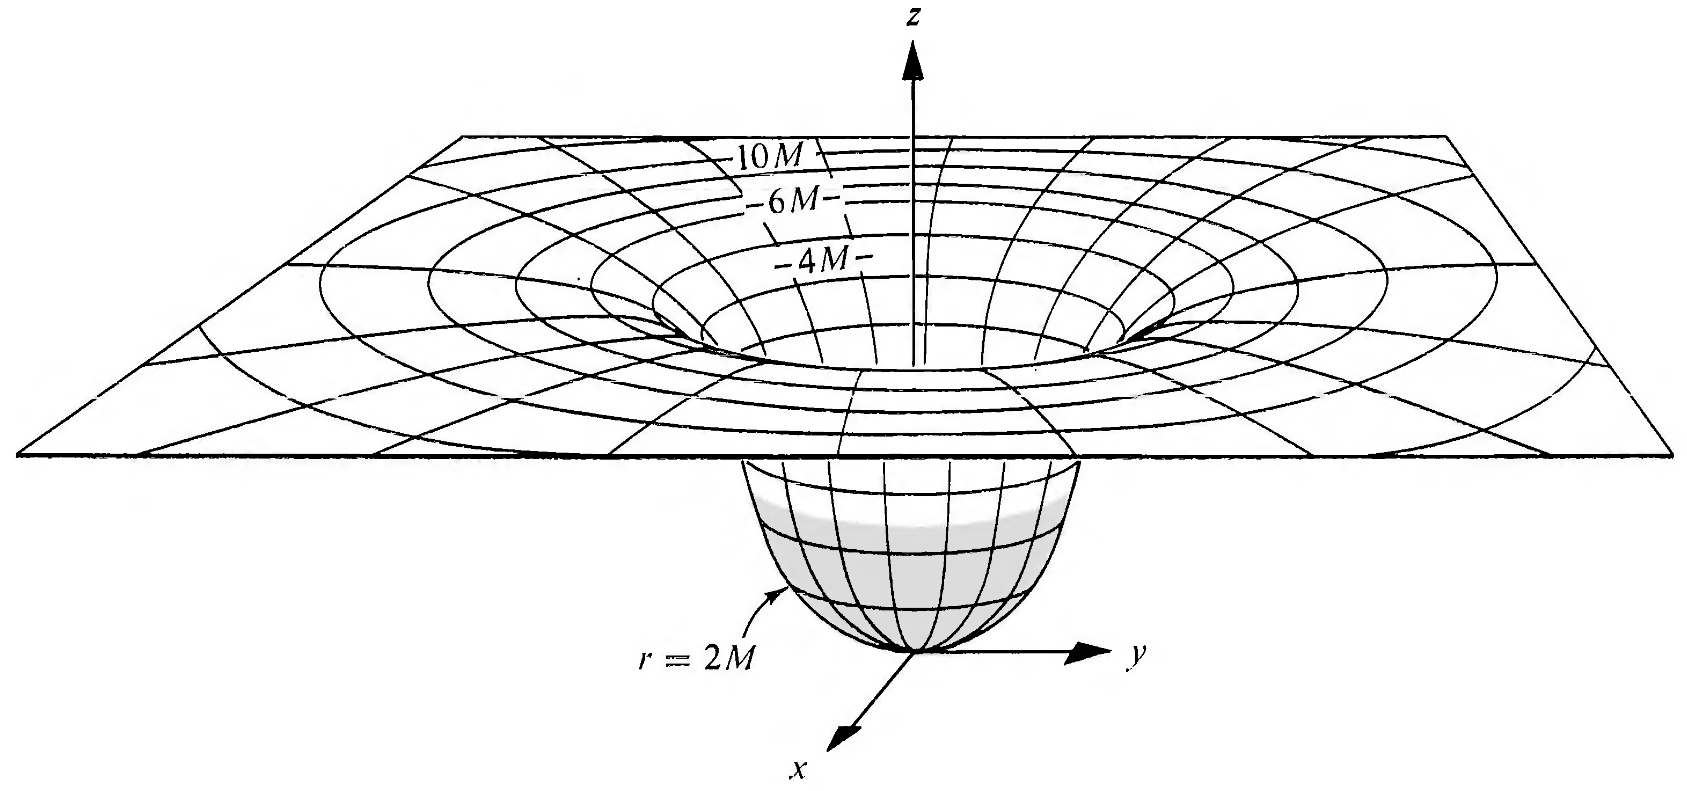
\includegraphics[align=t,width=\linewidth]{curvature1.png}%
\\[\jot]%
\footnotesize{\color{mpcolor}Energy, momentum, angular momentum are measures of particular curvatures of spacetime.}%
}%

\section{Entropy}
\label{sec:intro_entropy}

Entropy is a \emph{scalar} quantity, with SI dimension \textsf{energy$/$temperature}, and measured in units of \furl{https://doi.org/10.1351/goldbook.C01365}{\emph{joules}$/$\emph{kelvins} (\unit{J/K})}. From this definition it would seem that entropy is derived from temperature. However, although \textsf{temperature} is taken as primitive by the SI, the \furl{https://doi.org/10.1351/goldbook.K03374}{definition of temperature} actually depends on a fixed value of \furl{https://doi.org/10.1351/goldbook.B00695}{\emph{Boltzmann's constant}}, which has the dimension of \textsf{entropy}.

Entropy is probably the most difficult quantity to grasp intuitively. Many seemingly intuitive descriptions given in some textbooks are, unfortunately, unhelpful and even misleading.
\marginpar{\centering%
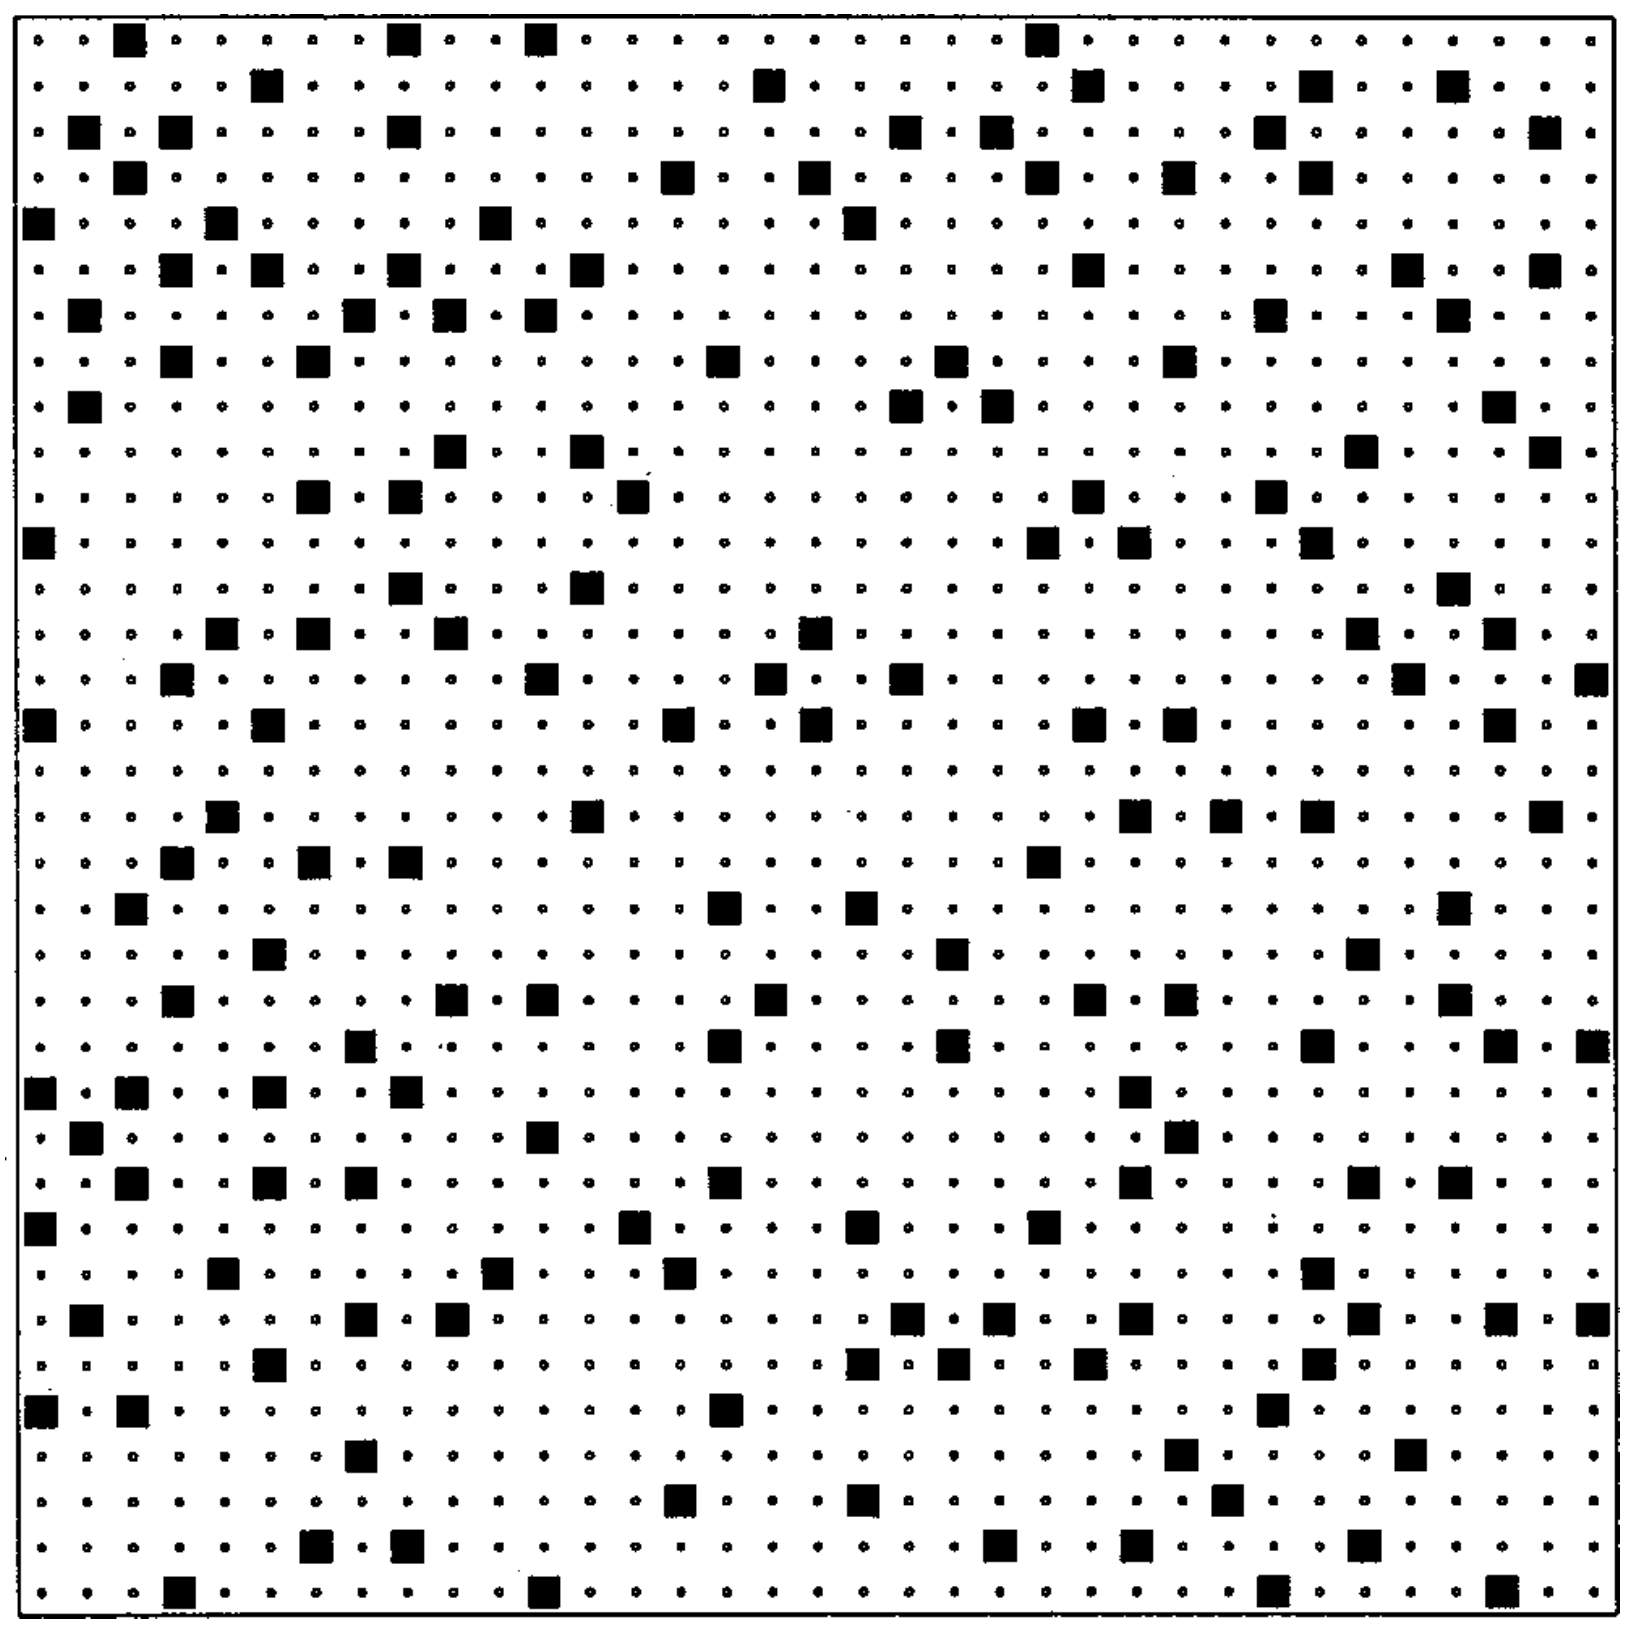
\includegraphics[align=t,width=1\linewidth]{entropy_low.png}\\%
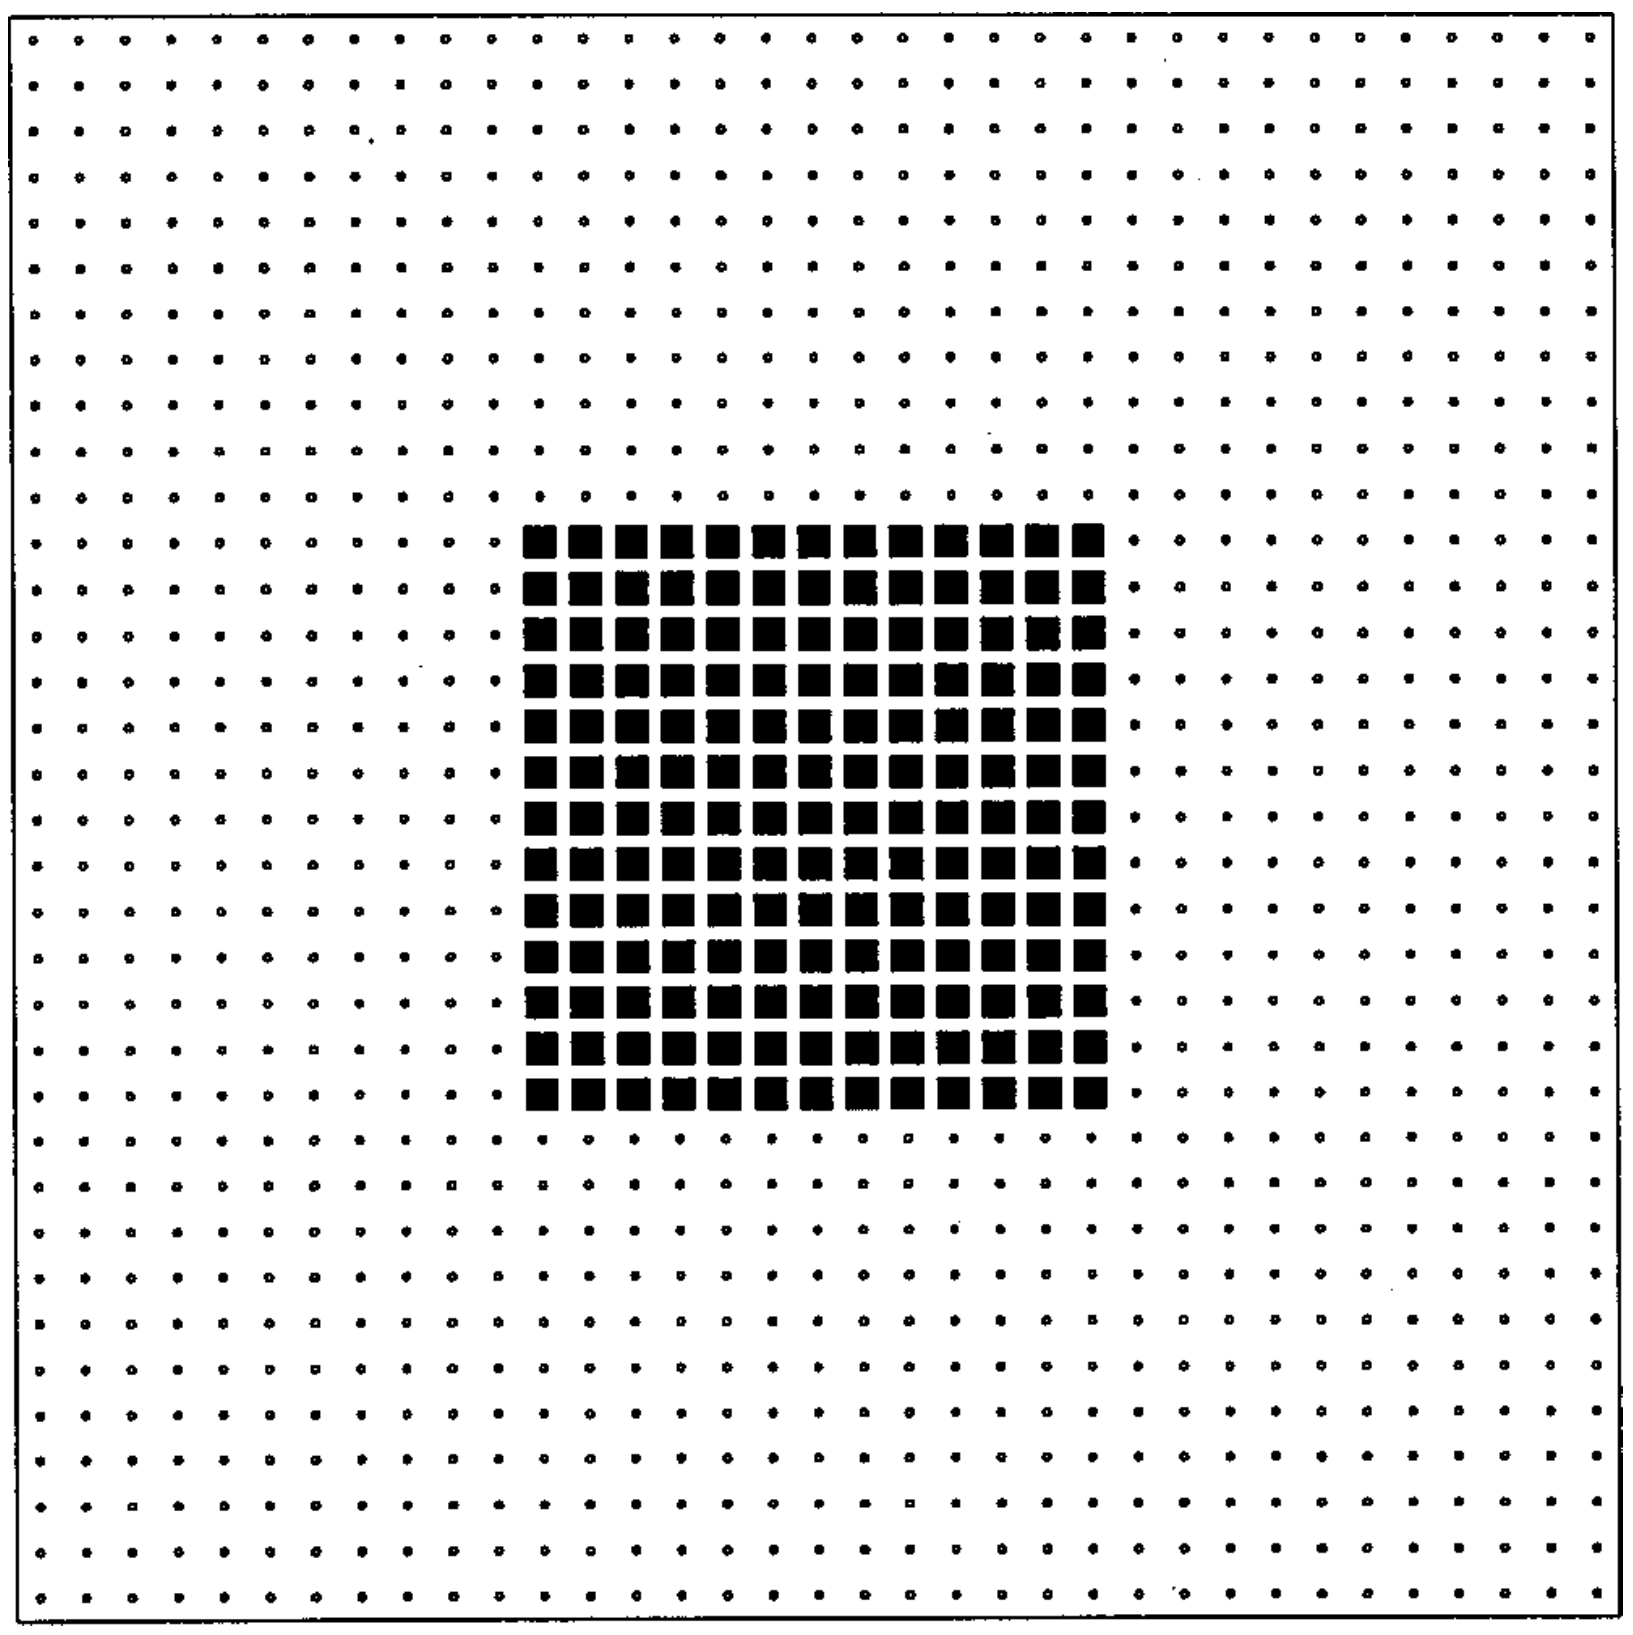
\includegraphics[align=t,width=1\linewidth]{entropy_high.png}
\\[\jot]\flushleftright%
\footnotesize{\color{mpcolor}Microscopic configurations of a lattice gas. \textbf{Left}: a configuration coming from a \emph{low}-entropy state. \textbf{Right}: a configuration coming from a \emph{high}-entropy state \parencites{styer2000}}.
}
One particularly misleading intuition is that entropy would be a \enquote{measure of disorder}. Besides the fact that \enquote{disorder} is very vague and subjective, it turns out that some physical phenomena, for example with \furl{https://www.britannica.com/science/liquid-crystal}{liquid crystals}, can be considered more \enquote{disordered}, and yet have \emph{lower} entropy, than others. See also the example in the side figure. We shall discuss more about such phenomena later on.

In these notes we shall rely on the idea that \emph{entropy expresses a limit on the flux of energy into matter}. Said in simpler but more imprecise words, entropy is a bound on how fast we can heat up a body. We shall develop this idea further later.

One reason why entropy is difficult to grasp intuitively is that it has very different physical and mathematical aspects depending on the spatial scales and physical theory that we use to describe physical phenomena.

In many \enquote{continuum} phenomena, that is, phenomena where the molecular constitution of matter is not visible or not taken into account, entropy is treated as a \enquote{stuff-like} quantity similar to energy or electric charge. But there are difficulties also in this case. For some phenomena, for example involving non-elastic materials such as a simple paper clip, it is possible to introduce several entropies having different values -- and not just because of a change in measuring scale -- all of which can serve their purpose perfectly fine.

In molecular phenomena involving statistical mechanics, on the other hand, entropy is no longer a physical notion, but a \emph{probabilitistic} and \emph{statistical} one, related to guesses and inferences that we make about the physical phenomenon. Yet from many points of view it has roles similar to those of the entropy used in continuum phenomena.

We shall see later that the physical laws for entropy have also a different status with respect to the laws for the other six main quantities: they are, so to speak, \enquote{laws about laws}.

\smallskip

\begin{definition}{Entropy: notation}
  The amount of entropy in a region is usually denoted with $\yS$. We shall see that the flux of entropy is tightly related to heat, and we won't need a special symbol for it.
\end{definition}


\section{Metric}
\label{sec:metric}

A very important quantity constitutes an eighth fundamental building block of all our physical theories: the \textbf{metric}. It is quite different from the seven fundamental quantities, from both a physical and a geometrical point of view. For instance it is \emph{not} an extensive quantity: we can't ask \enquote{what's the total amount of metric in this region?} -- it would be a meaningless question.

The metric characterizes our measurements of space and time. It's the object that allows us to calculate how much \emph{physical} time has elapsed, or the \emph{physical} distance of an object. In General Relativity it allows us to calculate the curvature of spacetime.

In the Newtonian approximation, that is, for speeds smaller than the speed of light and low energy densities (hence weak gravitational fields and small spacetime curvature), the metric is just a static, uniform background object, and spacetime has no curvature. This is why we can speak of an \enquote*{absolute time} and \enquote*{absolute distances} in this approximation. In these notes we shall for the most part use this Newtonian approximation.

In General Relativity the metric is a dynamic object instead: it can change in time, and can vary from region to region. These changes are determined by the seven fundamental quantities, and the metric, in turn, determines changes in the seven quantities.


\section{Auxiliary quantities}
\label{sec:aux_quantities}

Besides the seven principal quantities, other auxiliary quantities appear in some physical theories. Important examples are \textbf{temperature} and \textbf{strain}. Most auxiliary quantities are not extensive. For instance we cannot ask \enquote{what's the total amount of temperature in this region?}. We shall later discuss and use some auxiliary quantities, especially temperature.


The dimensions, units, and scalar or vector character of all quantities mentioned so far are summarized in table\,\ref{tab:units}.
\begin{table}[b]
  \centering
  \begin{tabular}{lll}
    \hline\\
    \textbf{Quantity}&\textbf{SI Dimension}&\textbf{Unit}
    \\[2\jot]
    Time&\textsf{time}&\emph{second}\;\unit{s}
    \\[\jot]
    Length&\textsf{length}&\emph{metre}\;\unit{m}
    \\[\jot]
    Temperature&\textsf{temperature}&\emph{kelvin}\;\unit{K}
    \\[2\jot]
    Matter&\textsf{amount of substance}&\emph{mole}\;\unit{mol}
    \\[\jot]
    Electric charge&\textsf{electric charge}&\emph{coulomb}\;\unit{C}
    \\[\jot]
    \textbf{Magnetic flux}&\textsf{magnetic flux}&\emph{weber}\;\unit{Wb}
    \\[2\jot]
    Energy&\parbox[t]{10em}{\textsf{energy},\\[0\jot] \textsf{mass}}&\parbox[t]{5em}{\emph{joule}\;\unit{J},\\[0\jot] \emph{kilogram}\;\unit{kg}}
    \\[7\jot]
    \textbf{Momentum}
    &\parbox[t]{10em}{$\textsf{force}\cdot\textsf{time}$,
      \\[0\jot]$\textsf{mass}\cdot\textsf{length}/\textsf{time}$,
      \\[0\jot]$\textsf{energy}\cdot\textsf{time}/\textsf{length}$}
    &\parbox[t]{5em}{\unit{N\cdot s},
      \\[0\jot]\unit{kg\cdot m/s},
      \\[0\jot] \unit{J\cdot s/m}}
    \\[12\jot]
    \textbf{Angular momentum}
    &\parbox[t]{10em}{$\textsf{force}\cdot\textsf{length}\cdot\textsf{time}$,
      \\[0\jot]$\textsf{mass}\cdot\textsf{length}^{2}/\textsf{time}$,
      \\[0\jot]$\textsf{energy}\cdot\textsf{time}$}
    &\parbox[t]{5em}{\unit{N\cdot m\cdot s},
      \\[0\jot]\unit{kg\cdot m^2/s},
      \\[0\jot] \unit{J\cdot s}}
    \\[12\jot]
    Entropy&\textsf{energy$/$temperature}&\unit{J/K}
    \\[2\jot]
    \hline
  \end{tabular}
  \caption{Dimensions and units of the main physical quantities used in these notes. Quantities in \textbf{boldface} are vectors, the others are scalars}\label{tab:units}
\end{table}
% \begin{table}[tb]
%   \centering
%   \begin{tabular}{lll}
%     \hline\\
%     \textbf{Quantity}&\textbf{Geometric character}&\textbf{Unit}
%     \\[2\jot]
%     Time&\textsf{scalar}&\emph{second}\;\unit{s}
%     \\[\jot]
%     Length&\textsf{scalar}&\emph{metre}\;\unit{m}
%     \\[\jot]
%     Temperature&\textsf{scalar}&\emph{kelvin}\;\unit{K}
%     \\[2\jot]\color{green}
%     Matter&\color{green}\textsf{scalar}&\color{green}\emph{mole}\;\unit{mol}
%     \\[\jot]\color{purple}
%     Electric charge&\color{purple}\textsf{scalar}&\color{purple}\emph{coulomb}\;\unit{C}
%     \\[\jot]\color{red}
%     \textbf{Magnetic flux}&\color{red}\textsf{vector}&\color{red}\emph{weber}\;\unit{Wb}
%     \\[\jot]\color{blue}
%     Energy&\color{blue}\textsf{scalar}&\color{blue}\parbox[t]{5em}{\emph{joule}\;\unit{J},\\[0\jot] \emph{kilogram}\;\unit{kg}}
%     \\[5\jot]\color{cyan}
%     \textbf{Momentum}&\color{cyan}\textsf{vector}&\color{cyan}\parbox[t]{5em}{\unit{kg\cdot m/s},\\[0\jot] \unit{J\cdot s/m}}
%     \\[5\jot]\color{yellow}
%     \textbf{Angular momentum}&\color{yellow}\textsf{vector}&\color{yellow}\parbox[t]{5em}{\unit{kg\cdot m^2/s},\\[0\jot] \unit{J\cdot s}}
%     \\[5\jot]\color{midgrey}
%     Entropy&\color{midgrey}\textsf{scalar}&\color{midgrey}\unit{J/K}
%     \\[2\jot]
%     \hline
%   \end{tabular}
%   \caption{Dimensions and units of the main physical quantities used in these notes. Quantities in \textbf{boldface} are vectors, the others are scalars}\label{tab:units}
% \end{table}


\printpagenotes*
\clearpage
\chapter{Fluxes and volume integrals}
\label{cha:total_flux}


\epigraph{\emph{%
For the sake of persons of these different types, scientific truth should be presented in different forms, and should be regarded as equally scientific, whether it appears in the robust form and the vivid colouring of a physical illustration, or in the tenuity and paleness of a symbolical expression.%
}}{J. Clerk Maxwell \cites*{maxwell1870}}


Recall that the \autoref{cha:stuff}{main seven quantities} -- matter, electric charge, magnetic flux, energy, momentum, angular momentum, and entropy -- have three common properties related to their measurement:
\begin{enumerate}\color{green}
\item[(1)] We can measure the amount of quantity within a three-dimensional region, at a specific time instant
\item[(2a)] We can measure the amount of quantity flowing through a two-dimensional surface during a time lapse\textellipsis
\item[(2b)] \textellipsis or alternatively we can measure the amount of quantity flowing through a two-dimensional surface \emph{per unit time}, at a particular time instant
\item[(3)]\label{item:extensivity}The amount in a volume consisting of separate volumes is equal to the total of the separate amounts. Similarly for the flux through separate surfaces.
\end{enumerate}

Let's give definite names to the measurements~(1) and~(2b):
\begin{definition}{volume integral and flux}
  We can call measurement~(1) the \textbf{volume integral} of the quantity, although we won't use this term very often.

  \smallskip

  Most important, we call measurement~(2b) the \textbf{flux} of the quantity. % Remember that in order to calculate the flux through a surface we need to specify how that surface is moving.
\end{definition}

\smallskip

These two notions and measurements are very intuitive; that's also why it's convenient to base our physics upon them. In this chapter we straighten some details about their definition and also about our intuition.

\section{Control volumes and control surfaces}
\label{sec:choice_surfaces}

A first question that comes to mind is: how are the volumes and surfaces chosen?

The choice of volume (and therefore of the surface bounding it) for a volume integral, and the choice of surface for a flux are \emph{completely arbitrary}, and they can be \emph{completely imaginary}. Since they are under our control, they are called \textbf{control volumes} and \textbf{control surfaces}.

For example, consider a classroom and the people in it. In your imagination you can divide the classroom into two halves, say the front and the rear half. You can then ask or measure simply by counting:\enspace
\begin{enumerate*}[label=(\arabic*)]
\item how many people are, right now, in the rear half;\enspace
\item how many people are crossing the imaginary division between the front and rear half during one minute, starting from now.
\end{enumerate*}

% The results of the two measurements above are numbers, which in general can be positive or negative, for scalar quantities; or vectors for vector quantities.
% % This number depends only on the chosen region, surfaces, and times.

\smallskip

A control volume and a control surface don't need to be static: they can move and deform.

In the case of a control volume, movement doesn't matter: the volume integral in a control volume \emph{does not depend on the instantaneous motion of the volume}. In fact we can even imagine a control volume that exists for just one time instant.

\marginpar{%
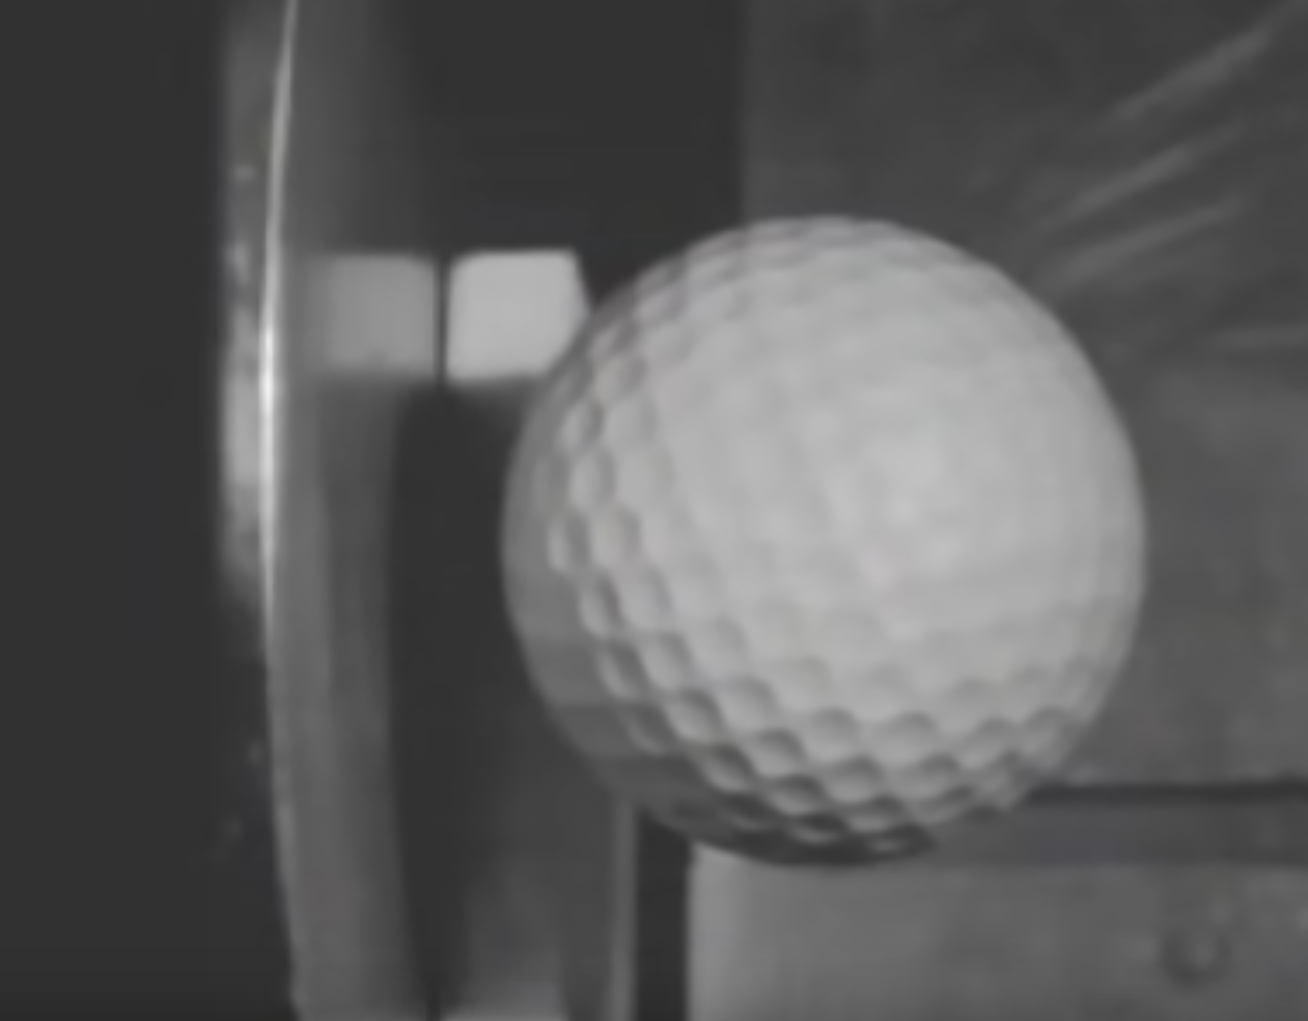
\includegraphics[align=c,width=\linewidth]{ball_wall.png}
\\[\jot]\flushleftright%
\footnotesize{\color{mpcolor}The golf ball is moving leftwards. Will it hit the metal surface? We don't know unless we know how the surface is moving.}%
}%
In the case of a control surface the situation is different. The flux through it \emph{depends also on the motion of the surface}. As a trivial example, consider a glass surface, and a person on one side of it, moving with a high velocity directed towards the surface. Will the person crash on the glass? We can't say for sure. The glass surface could be a glass wall in a building, which is not moving; in this case the person will likely crash on it. Or it could be the windscreen of a car, which is moving together with the person, who's the driver; in this case the person won't crash on it.

So we can't just imagine a surface that exists for one time instant: we need to imagine it for a very short time lapse, and be able to say how it's moving. If someone asks you what's the flux through a control surface at a given instant, but they don't tell you what's the motion of the surface, then the flux is unknown.


\smallskip

The fact that we can choose control volumes and control surfaces arbitrarily gives us a lot of power in solving physics problems and in making predictions. Typically they are chosen so as to simplify the equations that describe the physical situation, simulate physical phenomena in a more precise way, and focus on details of interest.
\marginpar{%
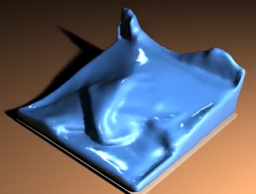
\includegraphics[align=c,width=\linewidth]{liquidvolume.png}
\\[\jot]\flushleftright%
\footnotesize{\color{mpcolor}Clever choice of control volume and surfaces allow us to model and predict complex motions of fluids; \furl{http://www.youtube.com/watch?v=M5xnAdVPbgQ}{see also animation} (\cites{wojtanetal2009})}%
}%

When we study some solid object, like a football, a rocket, or a planet, we typically choose a control volume that tightly encloses the object. When we study something flowing or moving, such as a fluid material or an electromagnetic field, we typically divide the space of interest into small control volumes and surfaces, constructing a \emph{mesh}; this mesh can even be refined in regions that are of special interest.

\section{Volume integrals: intuition and visualization}
\label{sec:intuition_volume}

\subsection{Scalar quantities}

A volume integral for a scalar quantity, for example energy, can be represented like this:
\begin{center}
  
\includegraphics[align=t,height=7em]{volumeintegral_8J.pdf}
\end{center}
we have eliminated one spatial dimension for simplicity, considering the analogous two-dimensional idea. The volume is in \textcolor{midgrey}{light grey}, delimited by a closed \textcolor{darkgrey}{darker grey} boundary, and we're indicating that the volume integral, that is, the amount of energy within, is \textcolor{blue}{\qty{8}{J}}.

As a visualization device, this representation can be useful. But let's straighten out some of its aspects:
\begin{itemize}[para]
\item Recall that this is a snapshot at a given time instant. So there are \qty{8}{J} of energy in the volume at that instant, but we don't know the situation earlier or later: there could be a different amount of energy, the region might be at a different position and have a different shape, or it might not even exist.

\item Recall that some scalar quantities, such as electric charge and in some situations matter (antimatter), can have negative amounts.
\marginpar{\centering%
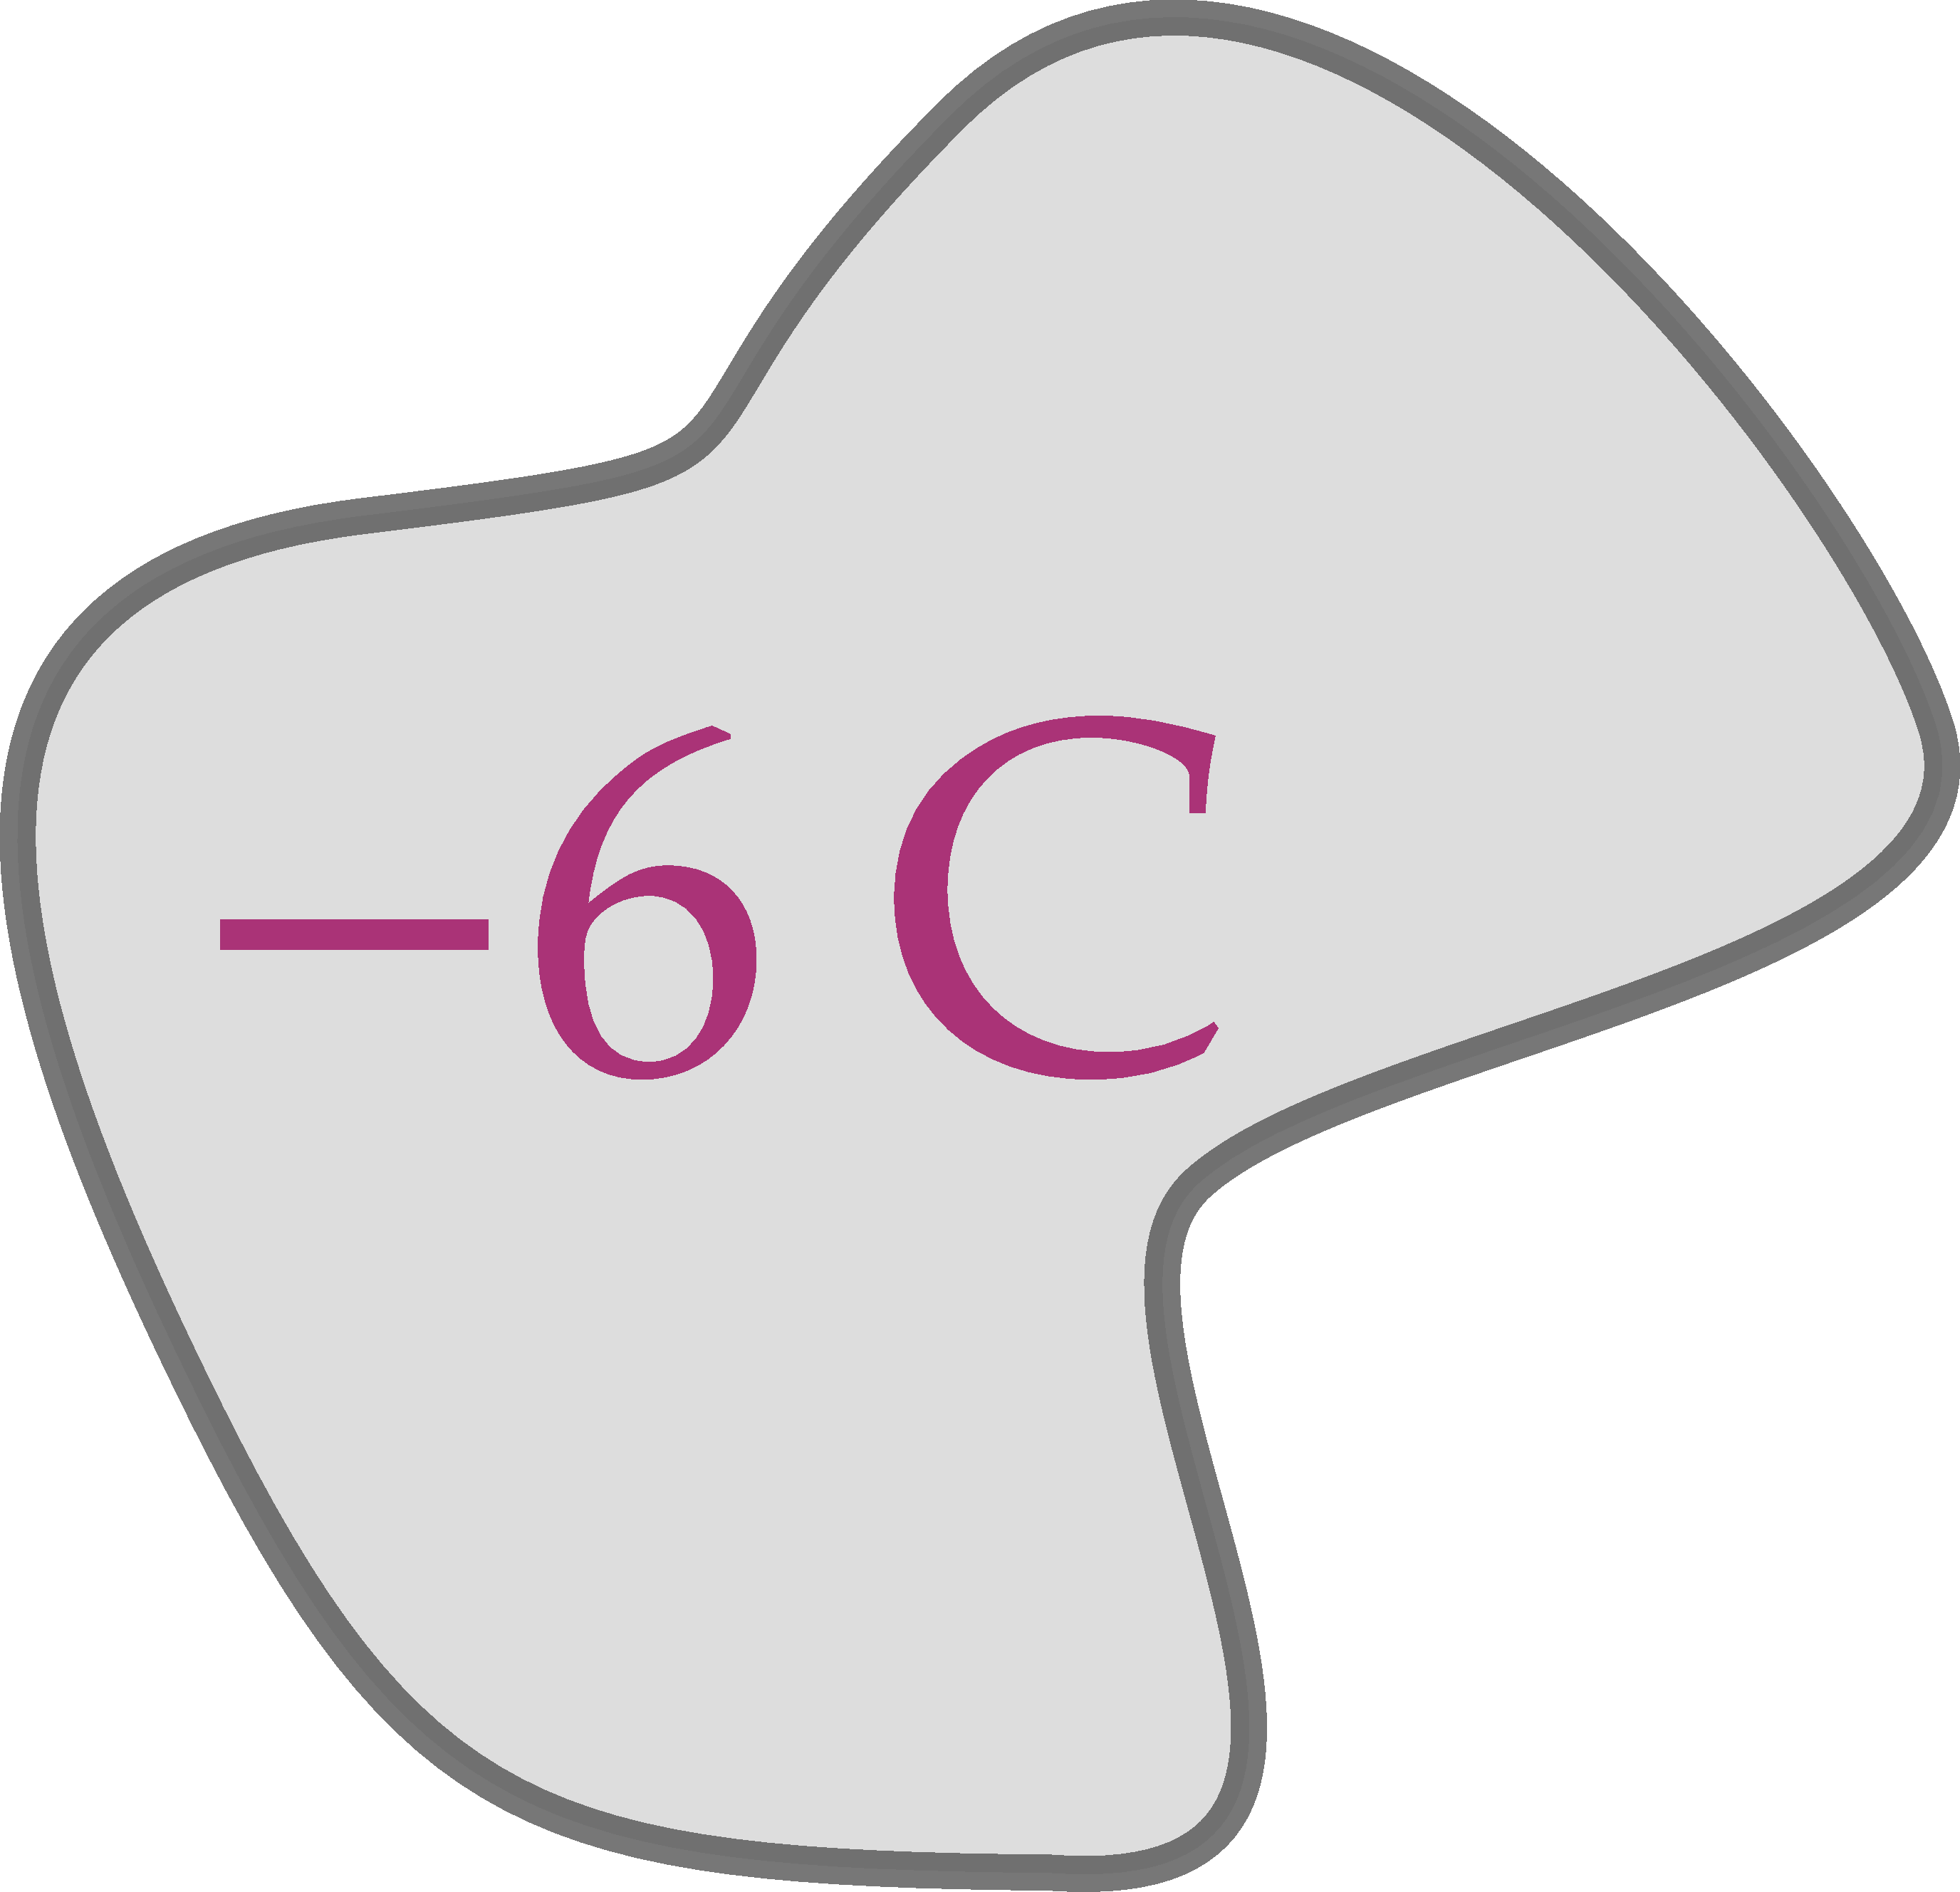
\includegraphics[align=c,width=0.5\linewidth]{volumeintegral_6C.pdf}
\\[\jot]\flushleftright%
\footnotesize{\color{mpcolor}A region with a negative amount of charge}
}

\item We must not surmise that the amount of quantity is uniformly distributed within the volume. In fact there could be negative amounts of it in some subvolumes and positive in others. In particular,  even if there is a zero amount of quantity in a volume, some subvolumes could have non-zero amounts: some positive and some negative, so that the total is zero.
  % \begin{warning}
  %  Even if there is a zero amount of quantity in a volume, some subvolumes could have non-zero amounts: some positive and some negative, so that the total is zero.
  % \end{warning}
\end{itemize}

\bigskip

\begin{exercise}
  The volume integral of matter in a particular volume is equal to \qty{36}{mol}. Can we conclude that the volume doesn't contain antimatter?
\end{exercise}


\subsection{Vector quantities}

A volume integral for a vector quantity, for example momentum, can be represented as follows (we still simplify our visualization to two dimensions):
\begin{center}
  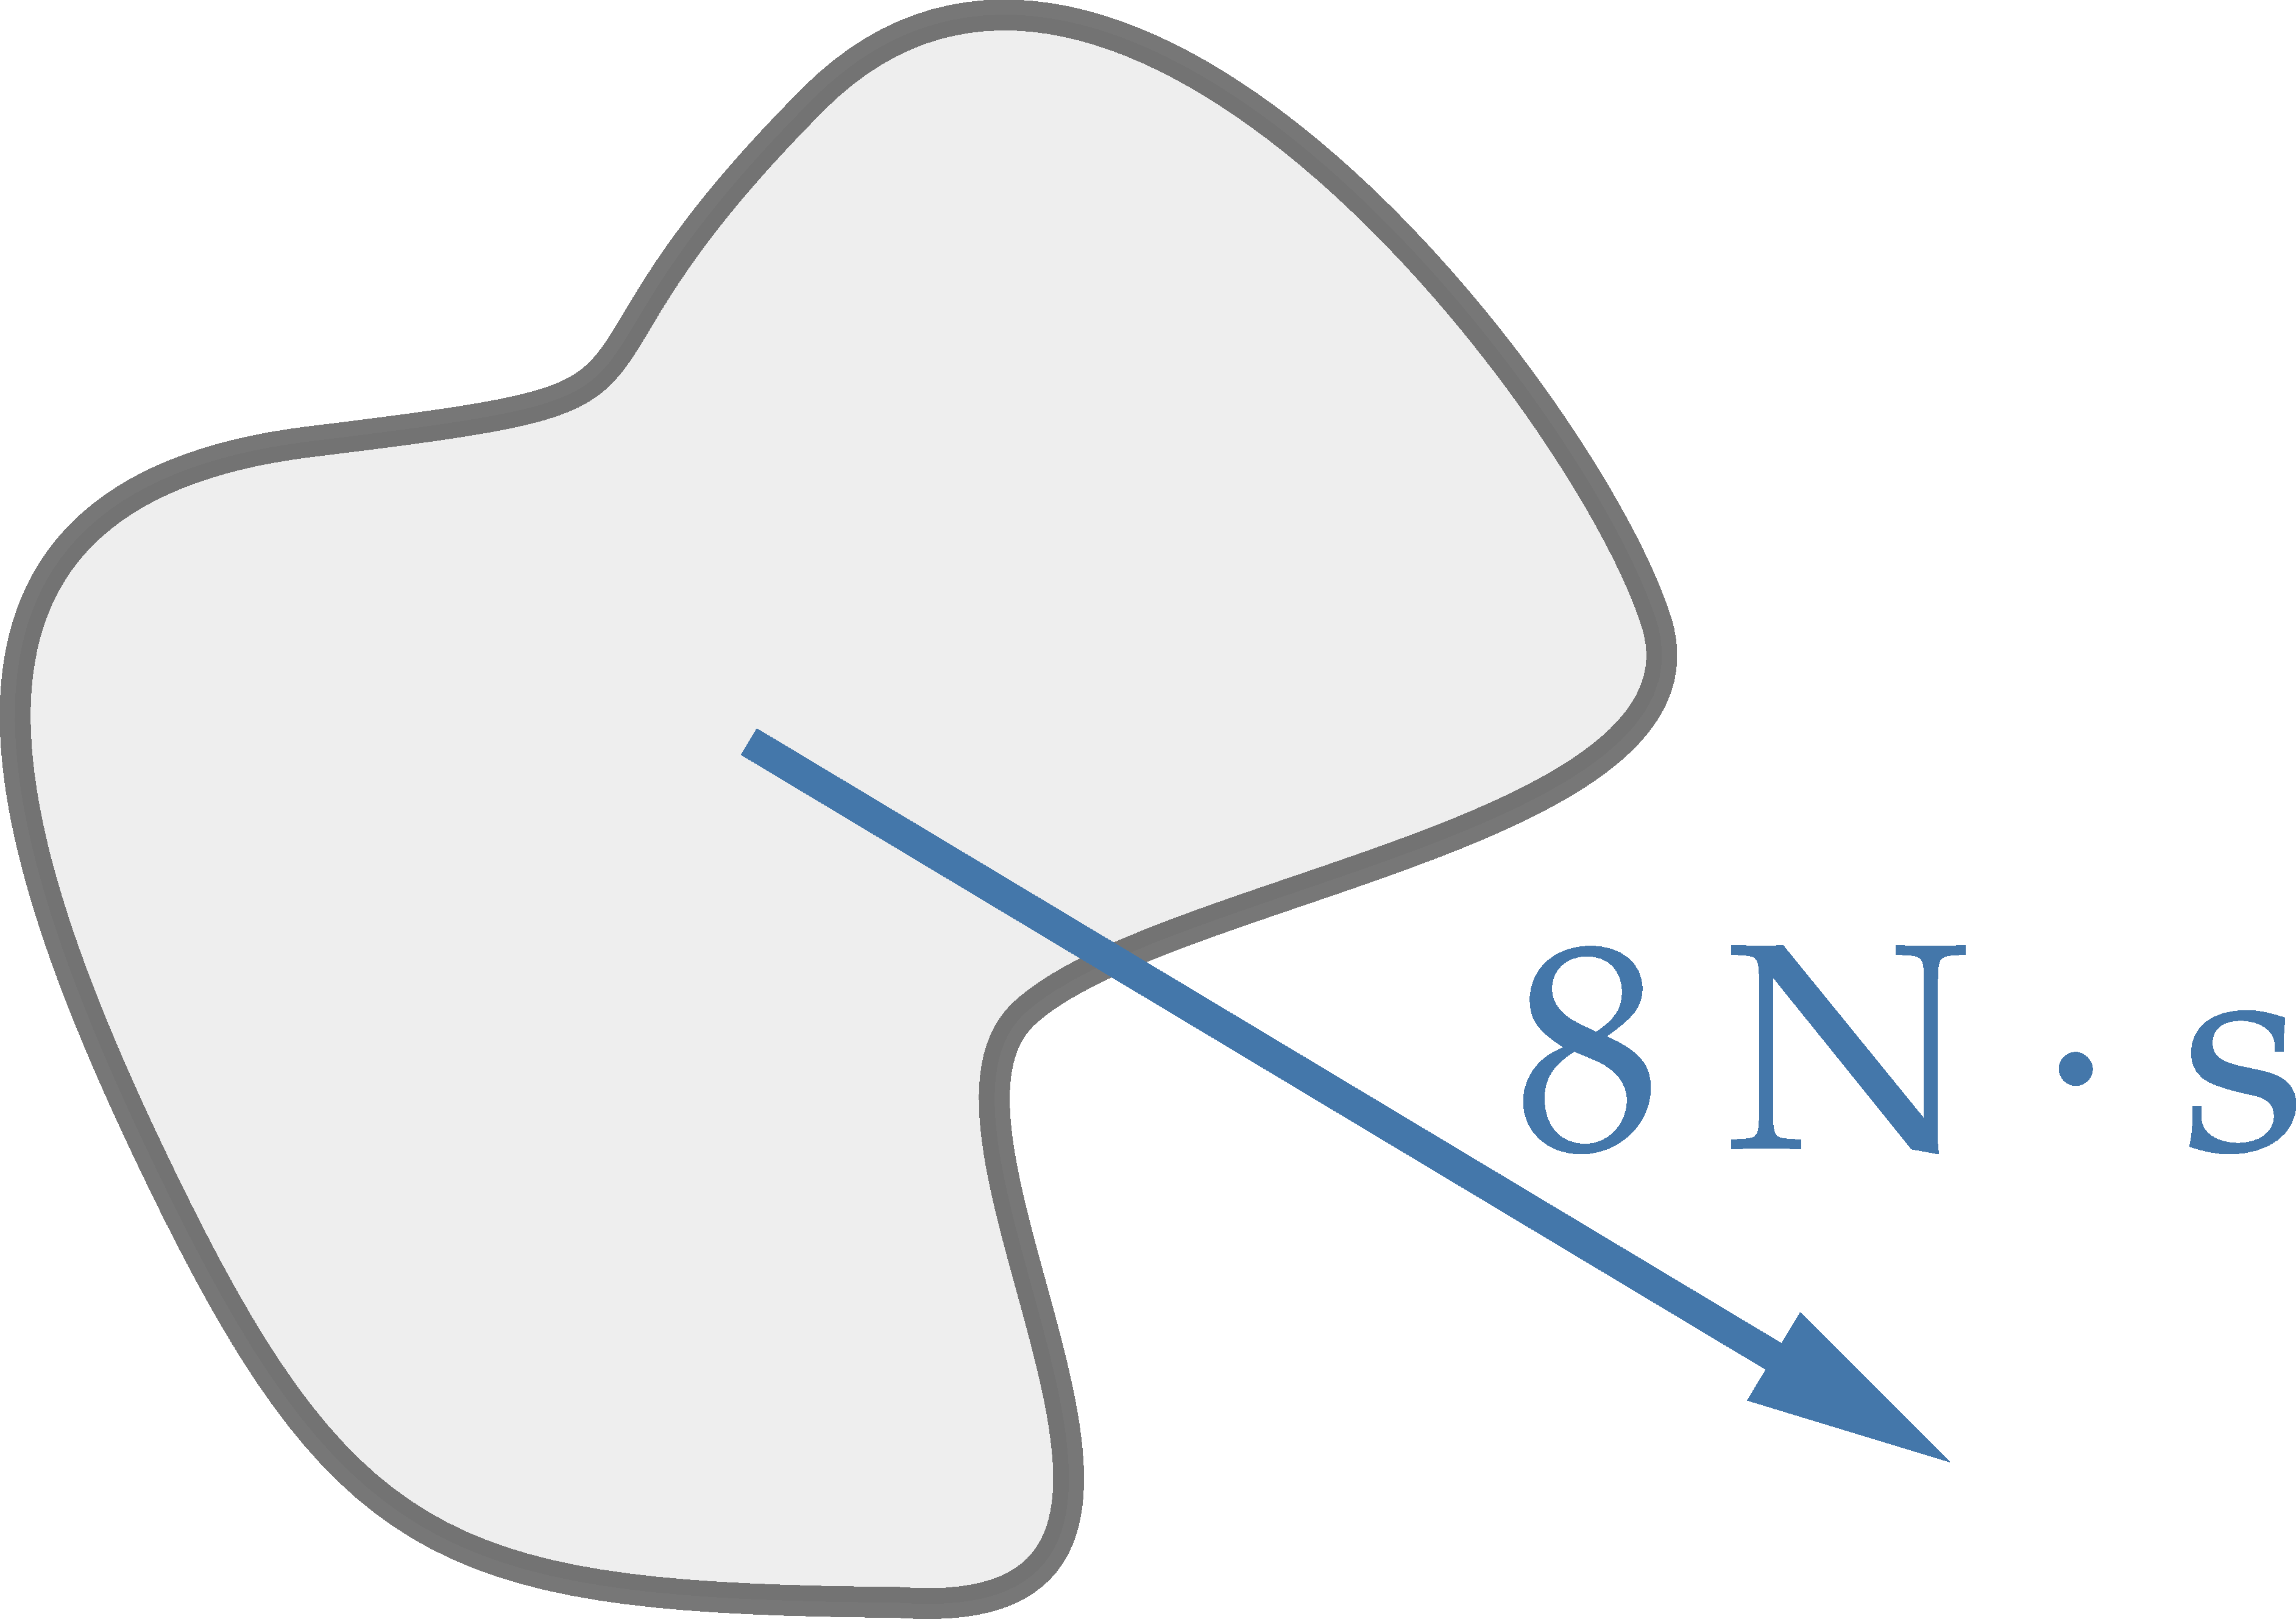
\includegraphics[height=7em]{volumeintegral_8Ns.pdf}
\end{center}
% \marginpar{\footnotesize
%   \begin{warning}%[Vector magnitudes are positive]
%     Remember that the \emph{magnitude} of a vector is always positive, and that\quad $\mathord{\mathcolor{purple}{\nwarrow}} = -1\cdot\mathord{\mathcolor{blue}{\searrow}}$
%   \end{warning}
% }
Momentum is a vector quantity, so the total amount in the volume above is a vector. The picture shows the direction and orientation of this vector, and the magnitude of \textcolor{blue}{\qty{8}{N\cdot s}}
is explicitly reported.
\begin{warning}[Vector magnitudes and opposite vectors]
  Remember that the \emph{magnitude} of a vector is always positive, and that\quad $\mathord{\mathcolor{purple}{\nwarrow}} = -1\cdot\mathord{\mathcolor{blue}{\searrow}}$
\end{warning}

The visual representation above is useful, if we keep in mind remarks analogous to the scalar case:
\begin{itemize}
\item This is a time snapshot.
\item\label{item:applicationpoint}The application point of the vector representing the volume integral is unimportant: for instance, it doesn't need to be placed at the centre of the volume. The vector refers to the volume as a whole, not to some specific point within.
\item Different subvolumes could have amounts represented by different vectors; only the total vector is represented above.
\end{itemize}
This last remark will be especially important when we discuss some physical phenomena involving rotation. As an example, look at the side picture:%\fig~\ref{fig:nonzero_vector_subregions}:
\marginpar{\vspace{-8\baselineskip}\centering%
\includegraphics[align=t,width=0.5\linewidth]{volumeintegral_N_divided.pdf}
\\[\jot]\flushleftright%
\footnotesize{\color{mpcolor}The whole region has zero volume integral. The left and right subregions have non-zero and opposite volume integrals.}%
}
the volume integral for the whole region is \emph{zero}, but its left and right subregions have \emph{non-zero and opposite} volume integrals.
% \begin{figure}[h]\centering
%   \includegraphics[height=7em]{volumeintegral_N_divided.pdf}
%   \caption{The whole region has zero volume integral. The left and right subregions have non-zero and opposite volume integrals.}\label{fig:nonzero_vector_subregions}
% \end{figure}

\smallskip


\begin{exercise}
  Recall the \autoref{item:extensivity}{third property of our seven main quantities}: The amount in a volume consisting of separate volumes is equal to the total of the separate amounts.

We have a region consisting of two subregions; the amounts of momentum in each subregion are shown below.
  \begin{center}
    \includegraphics[width=0.5\linewidth]{exercise_momentumsum.pdf}
  \end{center}
  \begin{enumerate}[shift,label=\bfseries\arabic*.]
  \item Write the total momentum in each subregion in component form, $(P_{x}, P_{y})$, according to the coordinate system shown.
  \item Calculate the momentum in the whole region; represent it graphically as vector and write it in component form.
  \end{enumerate}

  
\end{exercise}

\begin{extra}{Adding vectors in General Relativity}
 We are used to the idea of adding vectors placed at different points in space: we only have to first move each -- keeping it parallel to itself -- to a common point, and then add them all at that point with the usual rule.

  This operation \emph{cannot} be done in General Relativity: the notion of parallelism doesn't apply anymore in a simple way, owing to the curvature of spacetime. The addition would lead to different results depending on how we transported the vectors. So in General Relativity we can only sum vectors that are placed at the same spacetime point.

  How can this operation be possible in Newtonian mechanics and in practical applications, then? After all, General Relativity surely applies here! The answer is that the discrepancies of vector transportation are small enough in the neighbourhood of the Earth, as the curvature of spacetime is very small here.
\end{extra}


\section{Fluxes of scalar quantities: intuition and visualization}
\label{sec:intuition_fluxes_scalar}

\subsection{The direction, reckoning, and representation of scalar fluxes}
\label{sec:flux_scalar_direction}

Earlier we took the intuitive example of a flow of people through an open door; we might ask, for instance, how many people crossed the door in a minute. But one more detail about this flow is important: in which direction did the persons crossed the door? For example, if the door leads to a classroom, we may need to know whether the people who crossed the door got in or out, so as to know if there are seats left in the classroom.

In order to do this we can:
\begin{enumerate*}[label=\arabic*.]
\item Assign a crossing direction to the door, calling for instance \enquote*{positive} the direction from outside to inside the classroom.
\item Count as \enquote*{positive} each person who crosses the door in the positive direction, and count as \enquote*{negative} each person who crosses the door in the opposite direction.
\end{enumerate*}
The total tells us the \emph{net} number of people who \emph{entered} the classroom.
If the total is positive, then more people got in than out; if the total is negative, then more people got out than in.

One important aspect of this example and terminology is the following symmetry:
\begin{itemize}
\item What crossing direction is called \enquote*{positive} is fully arbitrary, just a matter of agreement.
\item If we decide to call \enquote*{positive} the other crossing direction, then the total will change sign. But the physical situation is of course still the same.
\end{itemize}
Therefore the sentences \enquote{\qty{+5}{persons} entered the room} and \enquote{\qty{-5}{persons} exited the room}
% \begin{itemize}\tightlist
% \item \qty{+5}{persons} entered the room
% \item \qty{-5}{persons} entered the room
% \item \qty{-5}{persons} exited the room
% \item \qty{+5}{persons} exited the room
% \end{itemize}
are saying exactly the same thing. This somewhat trivial fact about fluxes will, later on, turn out to be connected with a famous law.
So let's remember:
%
\begin{definition}{Every flux is equivalent to a flux of opposite amount in the opposite direction}
  A flux in a particular surface-crossing direction is equivalent to a flux of \emph{opposite} sign in the \emph{opposite} crossing direction.
\end{definition}
\marginpar{\vspace{-7em}\label{fig:newtonIII}%
\footnotesize\raggedright\color{mpcolor}\enquote{\emph{\langnohyph{LEX~III. Actioni contrariam semper \amp\ {\ae}qualem esse reactionem\,: sive corporum duorum actiones in se mutuo semper esse {\ae}quales \amp\ in partes contrarias dirigi.}}}
    \\\sourceatright{\cites{newton1687_r1726}}\par %\cites{newton1687_t1974}
}%

Another important aspect of the example above is that if we're told \enquote{\qty{-5}{persons} exited the room}, we don't know how exactly this happened: it could be that 5~persons got into the room during that minute; or that 10~persons got in and 5~got out; and so on. This is why we call \enquote*{\num{-5}} the \emph{net} amount.

Finally, consider a similar example but with a quantity that can ordinarily also be negative, such as electric charge. Call \enquote*{positive} the crossing direction from outside to inside the room. If we're told that a net charge amount of \qty{-5} crossed the door in the positive direction in one minute, then this could have happened in several ways:
\begin{itemize}\tightlist
\item a charge of \num{-5} was brought into the room
\item a charge of \num{+5} was brought out of the room
\item a charge of \num{-2} was brought into the room during the first \qty{30}{s}, and a charge of \num{+3} was brought out in the remaining \qty{30}{s}
\item a charge of \num{-2} was brought into the room during the whole minute, and a charge of \num{+3} was brought out at the same time
\item \textellipsis and many other possible combinations.
\end{itemize}
\marginpar{\footnotesize%
  {\color{mpcolor}\enquote{\emph{%
Fechner [in 1845] supposed every current to consist in a streaming of electric charges, the vitreous charges travelling in one direction, and the resinous charges, equal to them in magnitude and number, travelling in the opposite direction with equal velocity.}}\sourceatright{\cites{whittaker1910_r1951}}}%
}%
Indeed, ordinary electricity was  thought for some time to be associated with movements of negative \emph{and} positive charges in opposite directions.

\smallskip

The purpose of the examples and scenarios above is just to make you aware of some  aspects of what we shall call \enquote{flux}, which are trivial but important when considering fluxes of physical quantities.

How can we graphically represent the flux of a quantity, in such a way as to take care of these aspects? Consider these three representations:
\begin{center}\label{fig:scalar_fluxes}
\hspace*{\fill}\includegraphics[height=6em]{flux_plus5c.pdf}
\hfill\includegraphics[height=6em]{flux_minus5c.pdf}
\hfill\includegraphics[height=6em]{flux_minusplus5.pdf}
\hspace*{\fill}
\end{center}
The \textcolor{midgrey}{grey straight line} represents a surface (simplified to two dimensions) through which we're measuring a flux. In the first and second picture, the wavy arrows represent arbitrary crossing directions called \enquote*{positive}. The \textcolor{blue}{blue arrow} represents that we're calling \enquote*{positive} the left-to-right direction; the \textcolor{purple}{red arrow} represents that we're calling \enquote*{positive} the right-to-left direction. The signed number represents the net amount according to the positive direction -- so the first and second picture represent the same thing. One possible drawback of these two pictures is that they may suggest that a given amount is actually moving from left to right or vice versa; but we have seen that in general we don't know this.
The third picture tries to avoid this misleading suggestion by not showing any arrows; it is meant to represent that on the left side the amount of quantity has changed by \textcolor{purple}{\num{-5}}, and on the right side by \textcolor{blue}{\num{+5}}.

The third representation above has one more advantage. Remember that \autoref{sec:choice_surfaces}{a flux through a surface may occur because the surface itself is moving}. The wavy arrows in the first two representations above may misleadingly suggest that some amount of quantity is \enquote{moving} in their direction, or that the surface itself is moving in that direction. The third, arrow-less representation is less misleading.

In these notes we shall settle on the third representation above, but feel free to use the one you prefer -- as long as you are aware of all the important aspects of a flux.
\begin{warning}[What a flux does and doesn't tell]
  A flux tells us the net change in the amounts of a quantity on the two sides of a surface. These two amounts are equal in magnitude but have opposite signs.

  \smallskip

  A flux does \emph{not} tell us:
  \begin{itemize}\tightlist
  \item whether the quantity \enquote{was in motion}
  \item \textellipsis and if the quantity was in motion, what was its sign
  \item whether the surface was in motion
  \end{itemize}
\end{warning}

\subsection{How does a scalar flux change, if we change the surface?}
\label{sec:surface_change_scalar}

We know that the flux through a surface consisting of two smaller surfaces is the sum of the fluxes through the smaller surfaces. But what if we consider a \emph{different} surface, maybe intersecting the original one? It's important to keep in mind that \textbf{a flux refers to a particular surface, and can be very different if we consider a different surface, even if it's close to the original one}.

\pagebreak

Consider for instance the picture on the side.
%
\marginpar{\centering%
\includegraphics[align=t,width=\linewidth]{two_surfaces_flux.pdf}
}%
We have two intersecting surfaces (as usual simplified by removing one dimension), both almost horizontal. The energy flux through the \textcolor{blue}{solid blue surface}, in a roughly upward direction, is \textcolor{blue}{\qty{+5}{J/s}}. The energy flux through the \textcolor{purple}{dashed red surface}, again in a roughly upward direction, is instead \textcolor{purple}{\qty{-1}{J/s}}.

\smallskip

As another example,
%
\marginpar{\centering%
\includegraphics[align=t,width=0.67\linewidth]{two_surfaces_flux_eq.pdf}
}%
the new side picture shows two similar intersecting surfaces, one fully vertical in \textcolor{blue}{solid blue}, and one fully horizontal in \textcolor{purple}{dashed red}. The energy flux through the first in a rightward direction is \textcolor{blue}{\qty{+3}{J/s}}, and so is the energy flux in an upward direction through the second surface.



\subsection{Flux units: scalar quantities}

Remember that the flux of a quantity is defined as an amount of that quantity \emph{per time lapse}. Therefore the physical dimension of the flux is
\begin{equation*}
  \frac{\textsf{quantity}}{\textsf{time}}
\end{equation*}
and its units will be the units of the quantity divided by seconds:
\begin{definition}{units of fluxes of the four scalar quantities}
  \centering
  \begin{tabular*}{\linewidth}{@{\extracolsep{\fill}}lccccc}
    \textbf{quantity}&& matter & electric charge & energy & entropy
    \\[2\jot]
    \textbf{flux units}&& \unit{mol/s} & \unit{C/s} & \unit{J/s} & \unit{J/(K\cdot s)}
    \\[2\jot]
    \textbf{equivalent units}&& & \emph{ampere} \unit{A} & \emph{watt} \unit{W} & 
  \end{tabular*}
%  \caption{Units of scalar fluxes}
  \label{tab:fluxes_scalar_units}
\end{definition}

\bigskip

After our discussion about the peculiarity of fluxes it's quite easy to work with the fluxes of the four main scalar quantities: matter, electric charge, energy, entropy. Let us add some reminders and remarks about the fluxes of matter and energy.


\subsection{Matter flux}
\label{sec:matter_flux}

Remember that \emph{anti}matter \enquote{counts as \num{-1}} for calculating amounts of matter. If \qty{1}{mol} of positrons (anti-electrons) crosses a surface from left to right in \qty{1}{s}, the left-to-right flux equals \qty{-1}{mol/s} -- note the minus sign. The fact that antimatter is given special names can lead to ambiguities. For instance, if someone asks \enquote{what's the left-to-right flux of \emph{positrons}?}, maybe we should answer \enquote{\qty{1}{mol/s}}, since the question concerned specifically positrons. It's somewhat like asking \enquote{what's the flux of \emph{negative} electric charge?}. In these ambiguous situations is best to add some explanatory words.

\subsection{Energy flux}
\label{sec:energy_flux}
We already mentioned that \autoref{sec:forms_energy}{energy flux can be categorized into different kinds}, depending on whether there are fluxes of other quantities through the same surface. We study the exact definitions and formulae later on. The total flux is given by the sum of all these kinds. For instance, through a horizontal surface we can have a downward energy flux of \qty{3}{J/s} as \emph{heat}, and a downward flux of \qty{-1}{J/s} as \emph{work}. The total downward flux is then \qty{2}{J/s}. The energy flux that you will calculate in the fourth exercise below is called \emph{energy convection}.

\bigskip

\begin{exercise}
    For each question, answer in an \emph{unambiguous} way and sketch a picture representing the flux.
  \begin{enumerate}[shift,label=\bfseries\arabic*.]
  \item The two sides of a particular surface are called \enquote*{up} and \enquote*{down}. During \qty{0.2}{s}, an energy of \qty{+3}{J} flows from the up-side to the down-side, and an energy of \qty{-4}{J} flows from the down-side to the up-side. How much is the flux of energy through the surface?
  \item Through the same surface, at a later time, \qty{2}{mol} of neutrons flow from the up- to the down- side in \qty{0.01}{s}, and \qty{2}{mol} of neutrons flow from the down- to the up-side during the same time. How much is the flux of matter through the surface?
  \item The two sides of a surface are called \enquote*{in} and \enquote*{out}. During \qty{0.01}{s} there is a flow of \num{1000} electrons from the in-side to the out-side, and also a flow of \num{1000} \emph{positrons} (anti-electrons) in the same direction. How much is the flux of matter through the surface?
  \item The side picture shows a \textcolor{green}{surface} moving from left to right at a (constant) velocity of \qty{1}{m/s}. The space to its right has two static regions with some amount of \textcolor{blue}{energy} as shown (there's no energy behind to the left of the surface). How much is the flux of energy through the surface in \qty{1}{s}?
  \end{enumerate}
\end{exercise}
\marginpar{\vspace{-7\baselineskip}\centering\includegraphics[align=b,width=\linewidth]{surfacemoving_J.pdf}
}



\section{Fluxes of vector quantities: intuition and visualization}
\label{sec:intuition_fluxes_vector}

\subsection{The direction, reckoning, and representation of vector fluxes}
\label{sec:flux_vector_direction}

The flux of a vector quantity is also a vector, because it is given by an amount of that quantity, which is a vector, divided by time, which is a scalar.

The discussion about the \autoref{sec:flux_scalar_direction}{arbitrary choice of a crossing direction and the minus signs that appear when we reverse it} also applies, in an analogous way, to vector fluxes. Also the discussion about the minus sign remains the same; we must only remember that a minus sign changes the sense or orientation of a vector:
\begin{equation*}
  \mathord{\nwarrow} \mathrel{\enspace=\enspace} -1\cdot\mathord{\searrow}
\end{equation*}
Take for instance a horizontal surface. Suppose that we call \enquote*{positive} the \emph{upward} crossing direction, and that with this convection the flux is represented by the vector
\begin{center}
  \includegraphics[height=4em]{vec_NW.pdf}
\end{center}
Then if we decide to call \enquote*{positive} the \emph{downward} crossing direction instead, the same flux is represented by the opposite vector
\begin{center}
  \includegraphics[height=4em]{vec_SE.pdf}
\end{center}

The situation in the case of vector fluxes can require a little more thinking and attention, because it's easy to get confused between the crossing direction for the surface, and the direction suggested by the vector flux -- which are completely separate things. For this reason a good graphical representation of a vector flux is this, analogous to \autoref{fig:scalar_fluxes}{the third representation for scalar fluxes}:
\begin{center}
  \includegraphics[height=6em]{flux_vec_minusplus.pdf}
\end{center}
The \textcolor{midgrey}{grey straight line} represents a surface through which we're measuring the flux of a vector quantity; on the left side of the surface, the amount of quantity has changed by\enspace\includegraphics[align=c,height=1.5em]{vec_flux_left.pdf}\enspace and on the right side by\enspace\includegraphics[align=c,height=1.5em]{vec_flux_right.pdf}\:.
Obviously these two changes have equal magnitude but are opposite.

As a mental image of a vector flux, you can imagine a flow of vectors crossing the surface in one direction, together with a flow of opposite arrows crossing the surface in the opposite direction. \furl{https://pglpm.github.io/7wonders/media/vectorfluxanimsin.webp}{See this link} as an example.
%
\marginpar{\centering%
\includegraphics[align=b,width=0.5\linewidth]{vectorfluxanim.png}%
\\[\jot]\flushleftright%
\footnotesize{\color{mpcolor}Imagine the \textcolor{blue}{blue upper arrows} moving from left to right, and the \textcolor{purple}{red lower arrows} moving from right to left. \furl{https://pglpm.github.io/7wonders/media/vectorfluxanimsin.webp}{Animated version here}}.%
}%

\smallskip

Since a vector is represented by three numbers (which can be positive or negative), a vector flux can also be interpreted as the collection of three distinct numerical fluxes:
\begin{center}
  \includegraphics[height=6em]{flux_vec_minusplus_num.pdf}
\end{center}
the picture says that the $x$-component of the quantity has changed on the right side of the surface by \textcolor{blue}{\num{-21}}, and on the left side by \textcolor{purple}{\num{+21}}; the $y$-component  has changed on the right side by \textcolor{blue}{\num{+25}}, and on the left side by \textcolor{purple}{\num{-25}}; and the $z$-component hasn't changed on either side.

\medskip

Another aspect of vector fluxes that we must try not to get confused about is the application point of the vector representing the flux (the base point of the arrow). This is a time snapshot. Just like in \autoref{item:applicationpoint}{the case of vector volume integrals}, \textbf{the application point of the vector representing the flux is unimportant. The vector refers to one side of the surface as a whole.}

\medskip

\begin{exercise}
  A horizontal surface is given, and there is a flux of a vector quantity through it (for the moment we neglect units):
  \begin{enumerate}[label=\arabic*.]
  \item If we take the \emph{downward} crossing direction as \enquote*{positive}, the flux $xyz$-components are $(5,5,0)$. Represent this flux graphically, in the way discussed in the present section. Use the coordinate system\enspace\includegraphics[align=c,height=2em]{coords_xy.pdf}\enspace were $y$ points upward.
  \item Taking the same crossing direction, represent graphically the flux $(0,-2,0)$ instead.
  \item Taking the same downward crossing direction, we are now told that there is a flux with components $(1,-2,3)$. What are the components of this flux if we take the \emph{upward} crossing direction as positive?
  \end{enumerate}
\end{exercise}


\medskip

\subsection{How does a scalar flux change, if we change the surface?}
\label{sec:surface_change_scalar}

We saw that the flux of a scalar quantity can be very different if we take a slightly different surface. The same is true of the flux of a vector quantity: in particular, \textbf{the vectors representing the fluxes through two slightly different surfaces can point in completely different directions}.

Here is an example. Take a fixed point $P$. Now take a small vertical surface passing through $P$. The flux of a vector quantity (momentum for example) through this quantity can be as in this picture:
\begin{center}
  \includegraphics[align=c,scale=0.08]{skewfluxPx.pdf}
\makebox[0pt][c]{\hspace*{0.5\linewidth}\footnotesize(\furl{https://pglpm.github.io/7wonders/media/skewflux1.webp}{animated version})}
\end{center}
it has components $\mathcolor{blue}{(9,-6,0)}$, with magnitude around \num{10.8}, if we take the rightward crossing direction as positive.

Now forget about that surface, and take instead a small horizontal surface passing through the same point $P$. The flux -- of the same quantity -- through this surface can be as in this picture:
\begin{center}
  \includegraphics[align=c,scale=0.08]{skewfluxPy.pdf}
\makebox[0pt][c]{\hspace*{0.5\linewidth}\footnotesize(\furl{https://pglpm.github.io/7wonders/media/skewflux2.webp}{animated version})}
\end{center}
it has components $\mathcolor{blue}{(-6,-3,0)}$, with magnitude around \num{6.7}, if we take the upward crossing direction as positive.

Clearly the vectors representing the fluxes through these two surfaces are different: they point in different directions, and have even different magnitudes.

If we have a vector flux through a particular surface, and we're asked about the flux through a different surface, we might be tempted to \enquote{move} through the new surface the vectors representing the flux through the old one. \emph{We must fully resist this temptation}. It only leads to mistakes.
\begin{warning}[Each surface has a unique flux]
  A flux, scalar or vector, through a particular surface, in general doesn't tell you anything about the flux though another surface, even if the other surface is only slightly different from the first one.
\end{warning}

\subsection{Flux units: vector quantities}

Also for vector quantities the physical dimension of the flux is
\begin{equation*}
  \frac{\textsf{quantity}}{\textsf{time}}
\end{equation*}
and its units will be the units of the quantity divided by seconds:
\begin{definition}{units of fluxes of the three vector quantities}
  \centering
  \begin{tabular*}{\linewidth}{@{\extracolsep{\fill}}lcccc}
    \textbf{quantity}&& momentum & ang. momentum & magnetic field
    \\[2\jot]
    \textbf{flux units}&& \unit{N} & \unit{N\,m} & \unit{Wb/s}
    \\[2\jot]
    \textbf{equivalent units}&& &  & \emph{volt} \unit{V}
  \end{tabular*}
%  \caption{Units of scalar fluxes}
  \label{tab:fluxes_vector_units}
\end{definition}




\section{Flux of momentum: force}
\label{sec:force_is_flux}

We already mentioned that \autoref{sec:intro_momentum}{\textbf{flux of momentum is what we call \enquote*{force}}}. Owing to the importance of the notion of \emph{force} in the many branches of physics which rely on Newtonian mechanics, we must discuss this connection in depth. This connection, as well as the connection to Newton's laws, will become even clearer when we discuss the balance of momentum in \chap\,\ref{cha:bal_momentum}.

\subsection{Units}
\label{sec:units_momflux}

Recall that \autoref{sec:intro_momentum}{momentum can be measured in newton-seconds, \enquote*{\unit{N\cdot s}}}. Its flux, being a momentum per unit time, is therefore measured in newtons, \enquote*{\unit{N}}.

\subsection{Representing and visualizing force as flux of momentum}
\label{sec:visualize_force}

The notion of force is very intuitive. We associate it to the sensations that we feel in our skin, flesh, and even bones when, for instance, we push against a wall, twist a door knob, push backwards on the ground with our feet to run, or other similar actions. This force is typically represented by a vector, having the direction and orientation of the \enquote{push} or \enquote{pull}, and magnitude expressing its intensity. \emph{Such a force vector is exactly the vector expressing the flux of momentum}. The two are the same. A force can therefore also be visualized as a flow of momentum. This mental representation can be illuminating in some physical problems.

As a concrete example, imagine a person pushing against a wall. In terms of force, we say that \emph{the person is exerting a force on the wall,
  and the force vector on the wall has a person$\rightarrow$wall orientation}. This is usually depicted, for example, like this:%\noprelistbreak
\begin{center}
    \includegraphics[height=8em]{person_push_force.pdf}
\end{center}

In terms of momentum flux, we imagine a surface separating the person and the wall. If we take a person$\rightarrow$wall crossing direction, the flux vector also has a person$\rightarrow$wall orientation. Because of the symmetry of flux, if we take a wall$\rightarrow$person crossing direction instead, then the flux vector also changes direction. This momentum flux can be depicted (zooming in) like this:\noprelistbreak
\begin{center}
  \includegraphics[height=6em]{person_push_flux.pdf}
\end{center}
The picture says: on the side of the wall, momentum is changing by an amount having \textcolor{blue}{person$\rightarrow$wall orientation}; and, by symmetry of the flux,  on the side of the person's head, momentum is changing by an amount having opposite, \textcolor{red}{wall$\rightarrow$person orientation}.

\medskip

Let's take an example involving pulling instead of pushing. Imagine a person pulling a rope fastened somewhere. In terms of force we say that
\emph{the person is exerting a force on the rope,
  and the force vector on the rope has a rope$\rightarrow$person orientation}. This can be depicted like this:\noprelistbreak
\begin{center}
    \includegraphics[height=6em]{person_pull_force.pdf}
\end{center}

In terms of momentum flux, we imagine a vertical surface between the person's hand and the rope. If we take a hand$\rightarrow$rope crossing direction, the flux vector has a rope$\rightarrow$hand orientation -- note the difference from the previous example. Because of the symmetry of flux, if we take a rope$\rightarrow$hand crossing direction instead, then the flux vector has opposite direction: hand$\rightarrow$rope. This momentum flux can be depicted like this:\noprelistbreak
\begin{center}
  \includegraphics[height=6em]{person_pull_flux.pdf}
\end{center}
The picture says: on the side of the rope, momentum is changing by an amount having \textcolor{blue}{rope$\rightarrow$person orientation}; and, by symmetry of the flux,  on the side of the hand, momentum is changing by an amount having opposite, \textcolor{red}{hand$\rightarrow$rope orientation}.

\smallskip

A final example illustrates a situation in between the previous two. Consider the foot of a running person, as it pushes on the ground. In terms of momentum flux,
we imagine a horizontal surface between the runner's foot and the ground. If we take a downward crossing direction, the flux vector is oriented towards the back of the foot. Because of the symmetry of flux, if we take an upward crossing direction, then the flux vector has opposite direction, towards the front of the foot, the same as the running direction. This momentum flux can be depicted like this:\noprelistbreak
\begin{center}
  \medskip
  \includegraphics[height=6em]{foot_shear_flux.pdf}
\end{center}
The picture says: on the side of the ground, momentum is changing by an amount having \textcolor{blue}{leftward orientation}; and, by symmetry of the flux, on the side of foot, momentum is changing by an amount having \textcolor{purple}{rightward orientation}.


\subsection{Netwon's Third Law!}
\label{sec:newton_3rd}

%
\marginpar{%
\raggedright\footnotesize\color{mpcolor}%
        % \enquote{\emph{%
  %       \langnohyph{LEX~III. Actioni contrariam semper \amp\ {\ae}qualem esse reactionem\,: sive corporum duorum actiones in se mutuo semper esse {\ae}quales \amp\ in partes contrarias dirigi.}}}
  %       \\[\jot]
        \enquote{\emph{LAW~III. To every action there is always opposed an equal reaction: or, the mutual actions of two bodies upon each other are always equal, and directed to contrary parts.}}
        \\(Original Latin on p.~\pageref{fig:newtonIII})% \cites{newton1687_t1974}
        \\\sourceatright{\cites{newton1687_r1726}}
}%
From the examples above, we see that thinking of force as momentum flux automatically leads to \emph{Newton's third law}:
if one side is gaining/losing momentum with a given orientation, by symmetry the other side is gaining/losing momentum with the opposite orientation. So if one side is experiencing a force with a given orientation, the other side must be experiencing a force with the opposite orientation.

We see that Newton's third law is the expression of the symmetry of fluxes \emph{for the specific case of the flux of momentum (force)}. But we realize that this property is more general: it applies not only to force, but also to the flux of all other quantities, even scalar ones.



\begin{exercise}
  Using your intuition, try to guess the various momentum fluxes (except their magnitudes) between this person and the walls:\noprelistbreak
  \begin{center}
    \includegraphics[width=0.8\linewidth]{buster_electric_house.jpg}\\
    {\footnotesize\emph{(Buster Keaton in \furl{https://www.imdb.com/title/tt0013099/}{\enquote*{The Electric House}})}\par}
  \end{center}
\end{exercise}


\section{Pressure, tension, shear force}
\label{sec:pressure_tension_shear}

The examples of the previous section demonstrated a variety of possible orientations of the momentum-flux vector with respect to the surface through which it occurs. Obviously all orientations are possible. Special names are given, however, to a momentum flux having three specific orientations: \emph{pressure}, \emph{tension}, and \emph{shear force}.

Take a surface and call its sides $A$ and $B$. Now consider a flux of momentum according to the crossing direction $A\rightarrow B$.

\subsection{Pressure}
\label{sec:pressure}

If the momentum-flux \textcolor{blue}{from $A$ to $B$} is a vector also oriented from $A$ to $B$, then we call the momentum flux a \textbf{pressure}, or \emph{compressive momentum flux} or \emph{compressive force}. Here are two examples of pressure:
\begin{center}
  \hspace*{\fill}
  \includegraphics[align=c,height=6em]{pressure.pdf}
  \hfill
  \includegraphics[align=c,width=6em]{pressure2.pdf}
  \hspace*{\fill}
\makebox[0pt][c]{\hspace*{0.4\linewidth}\footnotesize(\furl{https://pglpm.github.io/7wonders/media/pressure.webp}{animated version})}
\end{center}
% \marginpar{\vspace{3\baselineskip}\centering%
% \includegraphics[align=t,width=\linewidth]{balloon.jpg}%
% \\\footnotesize\flushleftright{\color{mpcolor}%
% Spacetime representation of the evolution of a closed control surface, containing some pointlike objects (adapted from \cites{misneretal1970_r2017})}%
% }%


Pressure is the kind of momentum flux that we exert when we \emph{push} on an object, and that air exerts on all objects it surrounds.
% *** mynotew{add example with light and solar sails}
% *** any object in state of \enquote{compression}

\subsection{Tension}
\label{sec:tension}

If the momentum-flux \textcolor{blue}{from $A$ to $B$} is a vector oriented from $B$ to $A$, then we call the momentum flux a \textbf{tension}, or \emph{tensile momentum flux} or \emph{tensile force}. Here are two examples of tension:
\begin{center}
  \hspace*{\fill}
  \includegraphics[align=c,height=6em]{tension.pdf}
  \hfill
  \includegraphics[align=c,width=6em]{tension2.pdf}
  \hspace*{\fill}
\makebox[0pt][c]{\hspace*{0.4\linewidth}\footnotesize(\furl{https://pglpm.github.io/7wonders/media/tension.webp}{animated version})}
\end{center}

Tension is the kind of momentum flux that we experience in our bones when we \emph{pull} an object, and that occurs in any section of a stretched rubber band.
% *** any object in state of \enquote{tension}

\subsection{Shear force}
\label{sec:tension}

If the momentum-flux \textcolor{blue}{from $A$ to $B$} is a vector oriented transversally, along the surface itself, then we call the momentum flux a \textbf{shear force}, or \emph{shearing momentum flux}. Here are two examples of shear force:
\begin{center}
  \hspace*{\fill}
  \includegraphics[align=c,height=6em]{shearforce.pdf}
  \hfill
  \includegraphics[align=c,width=6em]{shearforce2.pdf}
  \hspace*{\fill}
\makebox[0pt][c]{\hspace*{0.4\linewidth}\footnotesize(\furl{https://pglpm.github.io/7wonders/media/shearforce.webp}{animated version})}
\end{center}

Shear force is the kind of momentum flux that we experience under our feet when we walk or run, and that occurs between a car's wheels and the ground.
% *** example with beams

\bigskip

In general, a momentum flux won't have any of the three special directions above, but rather a combination of them.


\begin{exercise}
  Using your intuition, try to identify the various momentum fluxes that occur in the different parts of a tower crane. Which of the fluxes are (approximately) compressive, tensile, and shearing?
\end{exercise}
\marginpar{\vspace{-8em}\centering%
\includegraphics[align=t,width=\linewidth]{towercrane.jpg}
}



\section{Closed surfaces, influxes, effluxes}
\label{sec:in_out_flux}

We shall often consider \textbf{closed} surfaces, that is, surfaces that don't have a rim or border or holes, like the surface of a sphere or of a cube. A closed surface delimits a specific three-dimensional volume, and we can naturally speak of its \textbf{interior} and its \textbf{exterior}. An example (simplified by removing one dimension as usual) is the surface in the side picture.
\marginpar{\centering%
\includegraphics[height=6em]{closed_surface.pdf}
}

% \begin{center}
%   \includegraphics[height=6em]{closed_surface.pdf}
% \end{center}

We can give two crossing directions to a closed surface: \emph{inward}, from exterior to interior; or \emph{outward}, from interior to exterior. A flux through the surface is usually called \textbf{influx} if we are considering the inward crossing direction, and \textbf{efflux} or \emph{outflux} if we are considering the outward crossing direction. Obviously, by the symmetry of fluxes,
\begin{equation*}
  \text{influx} \equiv -\text{efflux}
  \qquad\qquad
  \text{efflux} \equiv -\text{influx}
\end{equation*}

% Here is a depiction of an \emph{in}flux of \qty{2}{mol/s} of matter (equivalent to an efflux of \qty{-2}{mol/s}):
% \begin{center}
%   \includegraphics[height=7em]{closed_flux_mol.pdf}
% \end{center}

% \begin{warning}
%   It makes sense to speak of influx or efflux only for a \emph{closed} surface.
% \end{warning}

The influx and efflux are fluxes \emph{through the whole surface}. Consider for instance these fluxes of energy and of momentum:
\begin{center}
  \hspace*{\fill}
  \includegraphics[align=c,height=6em]{efflux_J.pdf}
  \hfill
  \includegraphics[align=c,height=6em]{efflux_N.pdf}
  \hspace*{\fill}
\end{center}
On the left we have an efflux of \qty{+5}{J/s} on the whole outer side of the surface. We don't know whether these \qty{5}{J/s} are being evenly distributed all around the surface, or just at particular spots of it. On the right we have an efflux of \qty{5}{N}, with a vector pointing approximately rightward. Again we don't know what are the flux vectors of individual pieces of the surface: the vector in the picture is just their total.

Let's see another example of this fact. The picture below on the left show the \textcolor{cyan}{outward fluxes} through three parts of a closed surface; the picture on the right shows the \textcolor{blue}{total efflux} through the same surface:
\begin{center}
  \hspace*{\fill}
  \includegraphics[align=t,width=0.4\linewidth]{flux_closed_3.pdf}
  \hfill
  \includegraphics[align=t,width=0.4\linewidth]{flux_closed_3_sum.pdf}
  \hspace*{\fill}
\end{center}
The individual fluxes and the total efflux are consistent, since
\begin{equation*}
  \mathcolor{cyan}{(2,-1,0)\:\unit{N}} +
  \mathcolor{cyan}{(0,4,0)\:\unit{N}} +
  \mathcolor{cyan}{(-2,-1,0)\:\unit{N}} =
  \mathcolor{blue}{(0,2,0)\:\unit{N}}
\end{equation*}



\bigskip


\begin{exercise}
  \begin{enumerate}[para,label=\bfseries\arabic*.]
  \item Are the four partial fluxes shown on the left consistent with the total efflux shown on the right? Why?:
    \begin{center}
  \hspace*{\fill}
  \includegraphics[align=t,scale=0.08]{flux_square.pdf}
  \hfill
  \includegraphics[align=t,scale=0.08]{flux_square_sum.pdf}
  \hspace*{\fill}
\end{center}

\medskip

\item  Take an imaginary cylindrical surface enclosing one \furl{https://energyeducation.ca/encyclopedia/Control_rod}{control rod} in a \furl{https://www.britannica.com/technology/nuclear-reactor}{nuclear-fission reactor} (side picture). Let's say that in a reactor there are 20 such rods. Approximately \num{5e19}~neutrons are liberated in a second in the whole reactor by the fission fuel, but 2/3 of these are \emph{absorbed} by the control rods.

  How much, on average, is the \textbf{ef}flux of neutrons (matter) through the surface of one control rod?

  Express the result first in \unit{neutrons/s}, and then in \unit{mol/s}, using the Avogadro constant $$N_{\textrm{A}} = \qty{6.02214076e23}{particles/mol} \ .$$ Be careful about the signs!
  % -1.7e18 n/s
  % -2.8e-6 mol/s
  \end{enumerate}
\end{exercise}
\marginpar{\centering%
\includegraphics[align=b,width=\linewidth]{nuclear_reactor.png}
% \\[\jot]\flushleftright%
% {\color{mpcolor}A region with a negative amount of charge}
}

% K: 0.86 g/cm^3 = 860 kg/m^3, aw=40*1.66e-27 kg
% 40K: 40+19=59
% NA=6.02214076e23
% 1.29518072289e38 particles/m^3
% 4400 Bq
% 3835e-28 m^2
% (1*pi*0.01)m^2
% 
% 500e6 J/s
% 7.2e13 J/kg
% 235 * 1.66e-27 kg/atom
% 3 neutrons/atom
% ((3 / (235 * 1.66e-27)) / 7.2e13) * 500e6
% 5.3405109801e19 neutrons/s
% 1.7801703267e19 neutrons/s at critical
% 8.9008516335e17
% 20 control rods
% approx 1e18 n/s
%
% 3e18 enter


\section{Integrated fluxes}
\label{sec:total_flow}

A flux is defined as the amount of a quantity crossing a surface in a short time lapse $\Dt$, divided by that time lapse. Denoting the flux by, say, $\yJ$, this definition also means that the amount of quantity crossing the surface in a short time $\Dt$ is equal to $\yJ\,\Dt$.

Take now a surface that exists between two time instants $t_{1}$ and $t_{2}$; during this time lapse it could also be moving and changing shape. Choose a crossing direction through the surface. At each intermediate time instant $t$ we can then measure the flux of a quantity crossing the surface in that direction, at that instant; denote it by $\yJ(t)$.

The total amount of quantity that crosses the surface between times $t_{1}$ and $t_{2}$ can be found by integrating $\yJ(t)$. That is, we divide the time interval into very short time lapses of length $\Dt$; for each short time lapse we know that the amount that crosses the surface is $\yJ(t)\,\Dt$. The total is obtained by adding these small amounts. As $\Dt$ is considered shorter and shorter, this sum is by definition an integral:
\begin{definition}{Integrated flux of a quantity through a surface between two times}
The total amount of quantity crossing a surface (relative to a specified crossing direction) between times $t_{1}$ and $t_{2}$ is given by
  \begin{equation}
    \label{eq:total_flow_integral}
     \int_{t_{1}}^{t_{2}}\!\! \yJ(t)\,\di t\ .
  \end{equation}
\end{definition}

The meaning of the integral above should be clear for any scalar quantity, for which the flux is also a scalar. In the case of a vector quantity, for instance momentum, the flux is also a vector, represented by three components. The integral of a vector is obtained by calculating the integral for each component, obtaining three results, which are the components of a new vector. Geometrically this corresponds to summing a large number of very small vectors.

Take the case of momentum, whose flux (force) we denote $\yF=(F_{x}, F_{y}, F_{z})$. The integral of this flux is then
\begin{equation}
  \label{eq:total_flow_integral_vector}
  \int_{t_{1}}^{t_{2}}\!\! \yF(t)\,\di t \defd
  \Biggl(
  \int_{t_{1}}^{t_{2}}\!\! F_{x}(t)\,\di t \ ,\enspace
  \int_{t_{1}}^{t_{2}}\!\! F_{y}(t)\,\di t \ ,\enspace
  \int_{t_{1}}^{t_{2}}\!\! F_{z}(t)\,\di t
  \Biggr) \ .
\end{equation}

\medskip

\begin{warning}[The integrated flux can be zero even with non-zero flux]
  The result of the integral defining the integrated flux can be zero. This means that no \emph{net} amount of quantity crossed the surface between $t_{1}$ and $t_{2}$. Yet the flux $\yJ(t)$ can be non-zero, even at all times; of course it needs to be positive at some times, and negative at others.
\end{warning}
As a simple example, consider a room's door. During one minute, three people enter through the door; during the next minute, three people (not necessarily the same) exit through the door. The total flow of people is zero, but the flux was non-zero during the first minute, and non-zero during the second minute.

\smallskip

\begin{exercise}
  \begin{enumerate}[shift,label=\bfseries\arabic*.]
  \item What is the physical dimension of the integrated flux of a quantity?
  \item Suppose that we calculate the integral above for a particular surface in the case of matter, finding a total of $\int_{t_{1}}^{t_{2}}\!\! \yJ(t)\,\di t = \qty{7}{mol}$. Now we change our mind and choose the opposite crossing direction for that surface. How does the result above change?
  \end{enumerate}
\end{exercise}

\section{Fluxes and velocities}
\label{sec:fluxes_velocities}

The idea of flux naturally evokes the idea of movement, and therefore of \emph{velocity}. Is there a relationship between flux and velocity?

The answer is yes: velocity is in fact essentially defined from a flux and a volume integral. Consider for example how we measure the velocity of an object: we are actually keeping track of a flow of matter from one region of space to another.

The rigorous definition of velocity from flux is somewhat involved, so here we'll just see a simplified and approximate example of how such a definition work. In any case, in the following chapters you won't need to remember any particular mathematical definition; just keep in mind that there's a tight connection between velocity, flux, and volume integral.

Take an extensive scalar quantity, like matter, charge, energy, or entropy. For concreteness let's think of matter. Take a coordinate system $(t,x,y,z)$ and a point in space at some specific time. Around this point choose a very small cuboid region, delimited by six small rectangular surfaces: two parallel to the $yz$-coordinate plane, two to the $zx$ one, and two to the $xy$ one. The cuboid has volume $V$, and the amount of matter (volume integral) in it is $\yN$. The flux through either one of the two $yz$ surfaces, crossing in the positive-$x$ direction, is $\yJ_{x}$, and either surface has area $A$. Note that if the cuboid is small enough, the flux through either of the two $yz$ surfaces, and their area, is approximately the same.

The $x$-component of the velocity of matter in this region is defined as
\begin{equation}
  \label{eq:velocity_from_flux}
  v_{x} \defd \frac{J_{x}/A}{\yN/V}
\end{equation}
with analogous definitions for the $y$- and $z$-components.
This definition is valid for small velocities and low energy concentrations (hence weak gravitational fields or spacetime curvature).


The velocity $\yv=(v_{x}, v_{y}, v_{z})$ so defined has the following intuitive property. If you choose \emph{any} very small surface centred at this point, and move it with this velocity (in the direction specified by the velocity), then the matter flux through it is zero. This reflects the intuitive understanding that if a surface is \enquote{moving} together with the matter, at the same speed, then we shouldn't observe any flux through it.

\marginpar{\vspace{2\baselineskip}\centering%
\includegraphics[align=t,width=\linewidth]{flux_velocity.pdf}
% \\[\jot]\footnotesize\flushleftright%
% {\color{mpcolor}A region with a negative amount of charge}%
}%
\begin{exercise}
  Try to prove the formula~\eqref{eq:velocity_from_flux} relating flux and velocity in an intuitive way, referring to the illustration on the side.

  As a starting point, consider this question: if the amount of matter $\yN$ in the volume $V$ is moving with velocity $v_{x}$ in the positive-$x$ direction, how much of it will cross the area $A$ during a time $\incr t$?
\end{exercise}

\medskip


\begin{extra}{Velocities of objects in general relativity}
  One consequence of the relationship between velocities and fluxes is that we can define such a velocity for any extensive quantity. So we have a velocity matter from the flux of matter, but also a \enquote{velocity of energy} from the flux of energy.

  In Newtonian approximation these two velocities are equal, so we do not need to distinguish them. In situations where the Newtonian approximation is not valid, on the other hand, we have to take into account the \enquote{velocity of matter} and the \enquote{velocity of energy} separately. This difference is important for instance in the study of plasma in stars and in numerical general relativity. There is an ongoing discussion as to which of the two velocities is more convenient to use; see for instance \cites{kandusetal2008}, especially the section \emph{Eckart frame versus Landau frame}, which refers to the choice between these two velocities.
\end{extra}

\section{Symbols for volume integrals and fluxes}
\label{sec:symbols_volint_flux}

Let us summarize the symbols for volume integrals and fluxes of the seven quantities, together with their units, that are used in these notes:
\begin{definition}{Symbols and units of volume integrals and fluxes}
  \centering
  \begin{tabular*}{\linewidth}{@{\extracolsep{\fill}}lcll}
    \textbf{quantity}&& \textbf{vol. integral}\enspace[unit] & \textbf{flux}\enspace[unit]
    \\[2\jot]
    matter&& $\yN$\enspace[\unit{mol}] & $\yJ$\enspace[\unit{mol/s}]
    \\[2\jot]
    energy&& $\yE$\enspace[\unit{J}] & $\yH$\enspace[\unit{J/s} \textcolor{grey}{\footnotesize or} \unit{W}]
    \\[2\jot]
    momentum&& $\yP$\enspace[\unit{N\,s}] & $\yF$\enspace[\unit{N}]
    \\[2\jot]
    angular momentum&& $\yL$\enspace[\unit{N\,m\,s}] & $\yT$\enspace[\unit{N\,m}]
    \\[3\jot]
    entropy&& $\yS$\enspace[\unit{J/K}] & $\yB$\enspace[\unit{J/(K\,s)}]
    \\[2\jot]
    \color{grey}\footnotesize electric charge&&\color{grey}\footnotesize (not used)\enspace[\unit{C}] &\color{grey}\footnotesize (not used)\enspace[\unit{C/s} \textcolor{grey}{\footnotesize or} \unit{A}]
    \\[2\jot]
    \color{grey}\footnotesize magnetic field&&\color{grey}\footnotesize (not used)\enspace[\unit{Wb}] &\color{grey}\footnotesize (not used)\enspace[\unit{Wb/s} \textcolor{grey}{\footnotesize or} \unit{V}]
  \end{tabular*}
%  \caption{Units of scalar fluxes}
  \label{tab:symbols_volint_fluxes}
\end{definition}




\clearpage

% \begin{equation*}
%   \incr t =
%   \sqrt{
%     \dfrac{
% 1- \frac{2\,G\,M}{R\,c^{2}}
%     }{
%     1
%     -\frac{v^{2}}{c^{2}}
%     -\frac{2\,G\,M}{(h+R)\,c^{2}}
%     -\frac{2\,G\,M}{(h+R)\,c^{2}}\,\frac{v^{2}}{c^{2}}
%   }}\,\incr\tau
% \end{equation*}
% \begin{equation*}
%   \begin{aligned}
%     M &= \text{mass of planet or star}\\
%     R &= \text{radius of planet or star}\\
%     h &= \text{altitude of satellite from surface of planet or star}\\
%     v &= \text{speed of satellite}\\
%   \end{aligned}
% \end{equation*}

\printpagenotes*
\clearpage
\chapter{Physical laws}
\label{cha:laws}


\epigraph{\emph{%
Every branch of physical science is based on two sets of fundamental equations. The first set is that of basic laws of physics, which are postulated to hold valid for all bodies under all conceivable circumstances \textelp{}. The second set of fundamental equations are the constitutive equations: these are relationships which are not supposed to hold for all bodies, but only to describe the behavior of some restricted class of bodies, or possibly of a larger class of bodies for a more restricted class of phenomena.
}}{G. Astarita \cites*{astarita1989_r1990}}

\section{Two kinds of laws}
\label{sec:two_kinds}

In \chap\,\ref{cha:stuff} we introduced seven main quantities in terms of which we describe physical phenomena. How do we describe the patterns, regularities, and diversities that we observe in these phenomena? This is the role of \emph{physical laws}. Different physics formalisms express physical laws in different ways, even if the actual physical phenomenon is exactly the same. In the formalism that we are using we distinguish between two kinds of physical laws:
\begin{definition}{Main distinction between two kinds of physical laws}
  \begin{itemize}
  \item\textbf{Fundamental laws} represent universal patterns that we observe everywhere. We shall see that there is a set of seven fundamental laws that apply on every known scale of space and time, and also across different physical theories.

\item\textbf{constitutive relations}  only apply to particular phenomena, only on particular time \amp\ space scales, only in particular theories. They express the diversity that we observe around us, and different kinds of approximations that we use in describing physical phenomena.
  \end{itemize}
\end{definition}

This distinction it's important. The fundamental laws can be applied with some confidence to every new phenomenon we observe, and often allow us to make predictions of at least a qualitative character. We only modify them as a last resort (which, so far, has been rarely or never necessary). We have a lot of freedom in modifying constitutive relations instead, and in proposing new ones to account for newly observed physical phenomena.

\medskip

As far as we know there is a very small number of fundamental laws and, remarkably, all known fundamental laws \emph{are balance laws}.
\begin{definition}{Balance and conservation laws}
  \textbf{Balance laws}, or simply \emph{balances}, have this name because they express a sort of trade-off or \enquote{budget} about physical quantities.

  \textbf{Conservation laws} are a special and important kind of balance laws.
\end{definition}
\marginpar{\vspace{-4\baselineskip}\centering%
\includegraphics[align=t,width=\linewidth]{physics_vs_magic.png}
\\\footnotesize{\color{mpcolor}%
\url{https://xkcd.com/2904}}%
}%


In this chapter we shall see how to mathematically express balance and conservation laws, as well as some kinds of constitutive relations.

\begin{warning}[\enquote*{Conservation} vs \enquote*{balance} in other texts]
  Be aware that many texts do \emph{not} distinguish between \enquote*{conservation law} and \enquote*{balance law}, and often use \enquote*{conservation} to mean both; which is unfortunate, since balance is the most general of the two. Always try to infer from the context how these two terms are used.
\end{warning}


\section{Conservation laws}
\label{sec:conservation_laws}

Conservation laws tightly connect \autoref{cha:total_flux}{\emph{volume integrals} and \emph{fluxes}}. They are intuitively and visually easy to grasp. The archetype is as follows:

Consider a \autoref{sec:in_out_flux}{\emph{closed} control surface} at a (coordinate) time $t_{1}$, which delimits a control volume. A spherical surface, delimiting a ball-shaped region, is an example. Actually the closed control surface doesn't need to be connected: it could consist of several separate closed control surfaces, each delimiting a different volume.

Starting from time $t_{1}$, imagine the closed control surface moving and deforming \marginpar{\vspace{-\baselineskip}\centering%
\includegraphics[align=t,width=0.245\linewidth]{cs1.png}\hfill%
\includegraphics[align=t,width=0.245\linewidth]{cs2.png}\hfill%
\includegraphics[align=t,width=0.245\linewidth]{cs3.png}\hfill%
\includegraphics[align=t,width=0.245\linewidth]{cs4.png}%
\\[\jot]\footnotesize\flushleftright{\color{mpcolor}%
Four snapshots of a moving and deforming closed control surface (\furl{https://pglpm.github.io/7wonders/media/volume_moving.gif}{click here for animated version})}%
}%
% \marginpar{\vspace{10\baselineskip}\centering%
% \includegraphics[align=t,width=\linewidth]{surfacemotion1.png}
% \\\includegraphics[align=t,width=\linewidth]{surfacemotion2.png}
% \\\includegraphics[align=t,width=\linewidth]{surfacemotion3.png}
% \\\includegraphics[align=t,width=\linewidth]{surfacemotion4.png}
% \\[\jot]\footnotesize\flushleftright{\color{mpcolor}%
%   Temporal sequence of closed control surfaces, represented by the golf ball's surface (\furl{https://pglpm.github.io/7wonders/media/surfacemotion.mp4}{click here for an animated version})}%
% }%
through time, changing shape and size but remaining closed -- no holes or cuts -- until a later time $t_{2}$. At this final time we have a final closed control surface that can be different from the initial one, and at a different position. If we wanted, we could start with a spherical surface delimiting a region the size of a tennis ball, and end with a cubical surface delimiting a region the size of the Sun. The temporal sequence of closed control surfaces delimits a sequence of control volumes; see the sequence on the side picture below as an example.

% The initial and final control volumes and the sequence of control surfaces in between are completely arbitrary. We choose them depending on the phenomenon that we want to study. They do not need to be the surfaces of real objects. For instance we can consider an imaginary cubical surface in the middle of a room, enclosing the air within; or in the middle of a river, enclosing, for an instant, the water within. But sometimes these arbitrary surfaces do coincide with the boundaries of objects. For instance we can consider the outer surface of a tennis ball, and follow it as the ball moves.

Now consider any one of the \autoref{sec:stuff}{seven primitive quantities}, except magnetic flux. Recall that these quantities are \emph{extensive}: we can measure the amount of this quantity in any control volume, and its flux across any control surface. For concreteness let's take \emph{matter}, for which we denote volume integrals by $\yN$ and flux by $\yJ$. We make the following measurements:
\begin{itemize}
\item $N(t_{1})$: total amount of matter contained within the control volume at time $t_{1}$.

\item $\yJ(t)$: \emph{\textbf{in}}flux (\autoref{sec:in_out_flux}{flux crossing inwards}) of matter (and antimatter!) through the closed surface at any particular time $t$ between $t_{1}$ and $t_{2}$.

\item $\yN(t_{2})$: total amount of matter contained within the control volume at time $t_{2}$.
\end{itemize}

Each of the three amounts above is, in this example, a scalar that can be positive, negative, or zero. For instance we could have:
\begin{equation*}
  \begin{gathered}
    t_{1} = \text{00:00:00}
    \qquad t_{2} = \text{00:00:18}
    \\ \yN(t_{1}) = \qty{3.50}{mol}
    \qquad \yJ(t) = -0.06\,t\:\unit{mol/s^{2}}
    \qquad \yN(t_{2}) = \qty{-6.22}{mol}
  \end{gathered}
\end{equation*}
note that $\yJ(t)$ is given as a function of the time $t$.
% The reason for changing the sign in the third measurement is that the surface is the final one through which we make the measurement; so, in a manner of speaking, this surface \enquote{points inwards through time} from a spacetime perspective.

% ; or a vector. For instance, for matter we could have $\yN(t_{1})=\qty{3.5}{mol}$; for energy we could have $\yJ=\qty{-600}{J}$; for momentum we could have $\bm{N}_{2} = (-3.4,0,+5)\,\unit{kg\cdot m/s}$.

\smallskip

With this setup we can introduce two kinds of balance laws.

\begin{definition}{Conservation law in integral form}
  An extensive quantity with volume integral $\yN(t)$ and influx $\yJ(t)$ is said to satisfy a \textbf{conservation law}, or to be \textbf{conserved}, if the following equality holds \emph{always}:
  \begin{equation}
    \label{eq:conserved}
    \yN(t_{2}) - \yN(t_{1}) - \int_{t_{1}}^{t_{2}}\!\!\yJ(t)\, \di t = 0
  \end{equation}
\end{definition}
The meaning of the equation above is intuitive, especially if we rewrite it like this:
\begin{equation*}
      \yN(t_{2}) = \yN(t_{1}) + \int_{t_{1}}^{t_{2}}\!\!\yJ(t)\, \di t
\end{equation*}
This expression says that the amount of quantity in the final control volume, $\yN(t_{2})$, is equal to the amount in the initial control volume, $\yN(t_{1})$, plus the total amount (which could be negative) that flowed in between those times, that is, the integrated flux $\int_{t_{1}}^{t_{2}}\!\!\yJ(t)\, \di t$. Said otherwise, any amount of quantity that appears in (or disappears from) the control volume, must come in (or go out) through the surface; it can't appear out of nowhere.

A conservation law allows us to make several kinds of predictions or deductions. For example:
\begin{itemize}
\item If we know the amount of quantity within the control surface at $t_{1}$ and the net amount that crossed the surface between $t_{1}$ and $t_{2}$, then we can predict the amount within the control surface at $t_{2}$: this is given by the last equation above.
  % \begin{equation*}
  %   \yN(t_{2}) = \yN(t_{1}) + \yJ \ .
  % \end{equation*}

\item If we know the amount of quantity within the control surface at $t_{1}$ and the one at $t_{2}$, then we can deduce the net amount that crossed the surface between the times $t_{1}$ and $t_{2}$:
  \begin{equation*}
    \int_{t_{1}}^{t_{2}}\!\!\yJ(t)\, \di t = \yN(t_{2}) - \yN(t_{1}) \ .
  \end{equation*}

\item If we know the amount of quantity within the surface at $t_{2}$ and the net amount that crossed the surface between $t_{1}$ and $t_{2}$, we can deduce the amount initially within the surface, at $t_{1}$:
  \begin{equation*}
    \yN(t_{1}) = \yN(t_{2}) - \int_{t_{1}}^{t_{2}}\!\!\yJ(t)\, \di t \ .
  \end{equation*}
\end{itemize}

These kinds of predictions and deductions are very powerful because we are fully free to decide the shape and motion of the control surface and volume, as well as the times $t_{1}$ and $t_{2}$.

We unconsciously use
several conservation laws all the time in our everyday life. If a bike tyre is suddenly deflated, we conclude that that air must have got out of it through it surface, which must therefore have a hole or a defective valve; we don't conclude that air \enquote{just disappeared}.
% If you seal a glass in a box, and upon dropping the box you hear that the glass shatters, and see that no holes were formed in the box, then you are sure that all the glass pieces now in the box could be glued together to form the original glass in its entirety.

% \begin{itemize}
% \item If we find a larger amount of the quantity within the surface at $t_{2}$ than the one at $t_{1}$, then the difference must have flowed in through the surface in between those times ($\yN(t_{2})-\yN(t_{1}) = \yJ$).
% \item If a total positive amount of the quantity is flowing in through the surface between times $t_{1}$ and $t_{2}$, then the amount of quantity within the surface at $t_{2}$ must be larger than the one at $t_{1}$ by this amount ($\yN(t_{1})+\yJ = \yN(t_{2})$).
% \end{itemize}
% You can think of other similar interpretations.

%% \mynotew{add more powerful ways by dividing regions, surface, time}

\smallskip

Note that the discussion so far is equally valid for a scalar or a vector quantity (we shall consider vector quantities more in detail in a moment).




\subsection{Differential form of conservation laws}
\label{sec:conservation_laws_diff}

The conservation law
\begin{equation*}
  \yN(t_{2}) - \yN(t_{1}) - \int_{t_{1}}^{t_{2}}\!\!\yJ(t)\, \di t = 0
\end{equation*}
is said to be written in \emph{integral form}, because it contains the integrated flux, necessary to calculate the net amount of quantity that crosses the control surface.

Change the symbol for time $t_{1}$ simply into $t$, and take $t_{2}$ to come after a \emph{very short} lapse of time $\Dt$ after $t$:
\begin{equation*}
  t_{1}\ \text{becomes}\ t\ ,\enspace t_{2}\ \text{becomes}\ t+\Dt
\end{equation*}
Then the integrated flux can be approximated by $\int_{t}^{t+\Dt}\!\!\yJ(t)\, \di t \approx \yJ(t)\, \Dt$ (because the flux $\yJ(t)$ is approximately constant in the short time lapse $\Dt$).

\marginpar{%
\footnotesize\flushleftright%
\begin{warning}
  Some mathematical conditions must be satisfied to make these steps; otherwise the derivative below must be carefully defined in a generalized sense.
\end{warning}\par
}%
The conservation law can then be approximated as
\begin{equation*}
  \yN(t+\Dt) - \yN(t) - \yJ(t)\, \Dt \approx 0
\end{equation*}
If we divide the whole expression by $\Dt$ and consider smaller and smaller $\Dt$, the fraction\enspace$\frac{\yN(t+\Dt)-\yN(t)}{\Dt}$\enspace becomes, by definition, a derivative, and we obtain a new form for the conservation law:
\begin{definition}{Conservation law in differential form}
  A quantity is said to satisfy a \textbf{conservation law} if the following equality holds always:
  \begin{equation}
    \label{eq:conserved_diff}
    \frac{\di\yN(t)}{\di t}- \yJ(t) = 0
  \end{equation}
\end{definition}
This form says that the rate of change of the volume integral of a quantity must equal \emph{\textbf{in}}flux of that quantity.

Both forms, integral and differential, of a conservation law are useful, in different situations. The integral form is obviously useful if we know the total flow during a time lapse but we don't know the flux at each instant. The differential form is often useful for simulating physical processes and make predictions.

\subsection{Example with a moving control surface}
\label{sec:example_conservation_moving}

\marginpar{\centering%
\includegraphics[align=t,width=\linewidth]{deflated_tyre.jpg}
% \\[\jot]\footnotesize\flushleftright{\color{mpcolor}%
%   Deflated tyre: did the air within just vanish out of existence?}%
}%
The tube within the tyre of a bicycle has, at a given time, \qty{12.6}{mol} of air.
The bicycle and its tyres moves around, and thirty minutes later the tyre is flat, the inner tube having only \qty{0.5}{mol} of air.

We consider an imaginary, closed control surface wrapping the tube. The control surface deforms just like the tube deforms. The initial control surface has therefore a tubular shape, but the final control surface doesn't.

We assume that air satisfies a conservation law. From the description above we have
\begin{equation*}
  t_{1}=\qty{0}{s} \ ,\quad
  t_{2}=\qty{1800}{s} \ ,\quad
  \yN(t_{1})=\qty{12.6}{mol} \ ,\quad
  \yN(t_{2})=\qty{0.5}{mol} \ .
\end{equation*}
The conservation law~\eqref{eq:conserved} allows us to calculate the integrated \textbf{in}flux:
\begin{equation*}
  \begin{split}
    \int_{t_{1}}^{t_{2}}\!\!\yJ(t)\,\di t &= \yN(t_{2}) - \yN(t_{1})
    \\&= \qty{0.5}{mol} - \qty{12.6}{mol}
    \\&= \qty{-12.1}{mol}
  \end{split}
\end{equation*}

\marginpar{\centering%
\includegraphics[align=t,width=\linewidth]{tyre_hole.jpg}
\\[\jot]\footnotesize\flushleftright{\color{mpcolor}%
There's a physical hole in the physical tube, but no holes in the imaginary control surface that wraps the tube}%
}%
The negative-signed result says that \qty{12.1}{mol} of air have crossed the moving control surface, in an outward direction, during thirty minutes. Obviously this happened because the tyre tube must have a hole.
Note that this is a physical hole in the physical tube; our control surface is imaginary and doesn't have any holes. It's just a sort of \enquote{border checkpoint} where anything can in principle move through; we only keep count of what's crossing, how much, and how fast.

We see that the fact that air satisfies a conservation law allows us to determine the integrated flux through the control surface. But it doesn't allow us to determine the flux $\yJ(t)$ at every individual time between $t_{1}$ and $t_{2}$. For example, we don't know if there was a larger flux at the beginning than at the end; the tyre may have gone completely flat just after \qty{60}{s}; in that case the flux $\yJ(t)$ was zero for $t>\qty{60}{s}$.

\subsection{Example with a static control surface}
\label{sec:example_conservation_static}

\marginpar{\centering%
\includegraphics[align=t,width=\linewidth]{waterblock.pdf}
% \\[\jot]\footnotesize\flushleftright{\color{mpcolor}%
% There's a physical hole in the physical tube, but no holes in the imaginary control surface that wraps the tube}%
}%
In the previous example we chose a closed control surface that moved and deformed with some object of interest (the tyre tube). But we can also choose a different control surface, for instance a static one.

Consider a block of \qty{53.4}{mol} of ice having cylindrical shape with \qty{1}{m} diameter and \qty{1.226}{m} height. It is falling downward owing to gravity (and in a vacuum). At a particular time it occupies a particular position; after \qty{0.5}{s} it is situated, for an instant, immediately underneath the initial position, as illustrated in the side picture.

Suppose we want to know the net quantity of ice that passed, in a downward direction, across the circular surface separating the initial and final positions. We can calculate this quantity by assuming that ice (as matter) satisfies a conservation law.

We choose a \emph{static} closed control surface of cylindrical shape.
\marginpar{\centering%
\includegraphics[align=t,width=\linewidth]{waterblock_control2.pdf}
% \\[\jot]\footnotesize\flushleftright{\color{mpcolor}%
% There's a physical hole in the physical tube, but no holes in the imaginary control surface that wraps the tube}%
}%
This control surface is located in such a way that it wraps the block of ice at the final time; at the initial time, therefore, the control surface is empty. See the side picture, where the control surface is represented by the \textcolor{yellow}{dashed yellow line}. This static control surface consists of three parts: a circular surface at the bottom, a side surface, and a circular surface at the top -- which is the one that interests us.

According to the description above we have
\begin{equation*}
  t_{1}=\qty{0}{s} \ ,\quad
  t_{2}=\qty{0.5}{s} \ ,\quad
  \yN(t_{1})=\qty{0}{mol} \ ,\quad
  \yN(t_{2})=\qty{53.4}{mol} \ .
\end{equation*}
From the conservation law~\eqref{eq:conserved} we calculate the integrated \textbf{in}flux:
\begin{equation*}
  \begin{split}
    \int_{t_{1}}^{t_{2}}\!\!\yJ(t)\,\di t &= \yN(t_{2}) - \yN(t_{1})
    \\&= \qty{53.4}{mol} - \qty{12.6}{mol}
    \\&= \qty{53.4}{mol}
  \end{split}
\end{equation*}
Note that this is the integrated influx through the \emph{whole} cylindrical surface. The conservation law doesn't tell us anything about the integrated influx through \emph{parts} of the surface. In the present case we provide the extra knowledge that the fluxes through the side and bottom surfaces are zero, between $t_{1}$ and $t_{1}$. Then, by the \autoref{def:extensivity}{extensivity property},
\begin{equation*}
  \begin{split}
    \int_{t_{1}}^{t_{2}}\!\!\yJ(t)\,\di t &=
    \int_{t_{1}}^{t_{2}}\!\bigl[\yJ_{\text{top}}(t) +
    \yJ_{\text{side}}(t) +
    \yJ_{\text{bot}}(t)\bigr]\,\di t
    \\
      \qty{53.4}{mol} &=
      \int_{t_{1}}^{t_{2}}\!\bigl[\yJ_{\text{top}}(t) +
      \qty{0}{mol/s} +
      \qty{0}{mol/s}\bigr]\,\di t
  \end{split}
\end{equation*}
from which we find, as was intuitively clear, that the net amount of ice that crossed the top surface in a downward direction is \qty{53.4}{mol}.

\bigskip

\begin{exercise}
{\itshape Solve the following exercises not just by using intuition, but \textbf{by explaining step-by-step how you use a conservation law}, in integral or differential form, to obtain the result:
\begin{itemize}\tightlist
\item what is the relevant time interval (if using the integral form)
\item how you define the closed control surfaces and their movement, as well as any subdivisions of the surfaces
\item what are the volume integral and integrated-flux values you know, and which you want to find
\end{itemize}}

\medskip

\begin{enumerate}[shift,label=\bfseries\arabic*.]
\item For the present exercise we assume that energy satisfies a conservation law.

  An apartment's room has two identical electric heaters along a wall. An electric heater can be considered as a piece of surface across which energy flows into the room: the energy is entering (through the electric cable) in the form of electromagnetic energy, and is converted into internal energy (mainly of the room's air) by means of the heater. Suppose that each heater corresponds to an influx of \qty{200}{J/s}.

    The room also has a window, which is the only other part of the room's boundary where energy can flow in or out.

    In one hour we measure that the total amount of energy in the room has not changed. How much is the integrated energy \emph{\textbf{in}}flux through the window during that time?

\medskip

%% *** check realistic values
  \item For the present exercise we assume that \furl{https://pubchem.ncbi.nlm.nih.gov/element/Argon}{argon} atoms satisfy a conservation law.

    A \furl{https://encyclopedia.che.engin.umich.edu/distillation-columns/}{distillation column} in a chemical plant has a constant influx of \qty{2}{mol/s} of argon atoms at one inlet, and a constant outflux of argon atoms, possibly at a different rate, at an outlet. An amount of \qty{500}{mol} of argon is measured in the chamber at a given time, and one minute later the amount is measured to be \qty{620}{mol}. How much is the argon \emph{\textbf{out}}flux (\emph{not} the integrated outflux) at the outlet?
  \end{enumerate}
\end{exercise}
\marginpar{\vspace{-24\baselineskip}\centering%
\includegraphics[align=b,width=\linewidth]{room_heater_window.jpg}
}
\marginpar{\vspace{-8\baselineskip}\centering%
\includegraphics[align=b,width=\linewidth]{distillation_column.jpg}
}




\section{Balance laws}
\label{sec:balance_laws}

Our intuitive understanding of a conserved quantity is that it cannot be \enquote{created} or \enquote{destroyed}. This leads to the definition of a more general law where this condition is not necessarily satisfied.

The setup is just like before: consider an initial and final closed control surfaces and volumes at $t_{1}$, $t_{2}$, and a sequence of closed control surfaces in between. This time let's take \emph{\energym} as a concrete example, with initial volume integral $\yE(t_{1})$, final volume integral $\yE(t_{2})$, and influx $\yH(t)$.

\begin{definition}{Balance law}
  A quantity with volume integral $\yE(t)$ and influx $\yH(t)$ is said to satisfy a \textbf{balance law}, or to be \textbf{balanced}, if the following equality holds \emph{always}:
  \begin{equation}
    \label{eq:balanced}
    \yE(t_{2}) - \yE(t_{1}) - \int_{t_{1}}^{t_{2}}\!\!\yH(t)\, \di t = \int_{t_{1}}^{t_{2}}\!\!\yR(t)\,\di t
  \end{equation}
  where $\yR(t)$, called the \textbf{supply} or \textbf{source}, is the amount of quantity created per unit time within the closed control surface at time $t$.
\end{definition}
If the quantity is a scalar, then $\yR(t)$ can also be negative, in which case we may call it a \emph{sink} and we say that some of the quantity is being destroyed at time $t$.

\smallskip

According to the definition above, a conservation law is a \emph{special, powerful case} of a balance law: one for which $\yR(t)=0$ \emph{always and everywhere}; that is, there never are sources or sinks of the quantity. It is powerful because the supply $\yR(t)$ is already known and has an extremely simple value (zero).

For this reason, a balance law is in some respects more trivial than a conservation law. If we measure that\enspace$\yE(t_{1}) - \yE(t_{2}) - \int_{t_{1}}^{t_{2}}\!\yH(t)\, \di t$\enspace is not zero (so there's no conservation law), we can always say that some amount of quantity must have been created or destroyed within the control volume between $t_{1}$ and $t_{2}$.\enspace An extensive quantity can therefore always be said to satisfy a balance. A balance is not trivial, however, if we have some specific physical law that tells us in advance how the amount created or destroyed at each instant, $\yR(t)$, can be calculated.

\marginpar{\centering%
\includegraphics[align=b,width=\linewidth]{tennisball_boundary.png}%
\\\footnotesize\flushleftright{\color{mpcolor}%
A conservation law only involves what happens within the initial and final control volume (represented by the \textcolor{red}{red hatched} disks), and on the sequence of control surfaces in between (represented by the curved \textcolor{red}{red} lines), but not what happens within the control volumes in between}%
}%
A conservation law is therefore powerful also because it allows us to predict the amount of quantity in the final volume by making measurements \emph{only on the surface} during the time lapse. A general balance law, instead, requires us to also make measurements at every point \emph{within the volume} during the time lapse.
\begin{warning}[Supplies are very different from fluxes]
  One could object: \enquote{why don't you just put the flux $\yH(t)$ and the supply $\yR(t)$ together, adding the two integrals in equation~\eqref{eq:balanced}? Wouldn't you get
  \begin{equation*}
    \yE(t_{2}) - \yE(t_{1}) - \int_{t_{1}}^{t_{2}}\!\!\bigl[\yH(t)+\yR(t)\bigr]\, \di t = 0
  \end{equation*}
  which looks like a conservation law?}

\smallskip

Unfortunately the mathematical expression above wouldn't be a conservation law, despite its appearance. The point is this: the flux $\yH$ involves only what's happening \emph{on the control surface}; the supply $\yR$, on the other hand, involves what's happening \emph{within the control volumes, at each time}. A conservation law involves only fluxes within the integral. That is, it doesn't require us to know what's happening within the control volumes, except at the initial and final time.
% Said otherwise, the integral $\int_{t_{1}}^{t_{2}}\!\!\yR(t)\,\di t$ is not an integrated flux.
\end{warning}


% A balance law allows us to make several kinds of predictions or deductions as well. For example:
% \begin{itemize}
% \item If we know the amount of quantity within the surface at $t_{1}$, the amount that flowed in through the surface between $t_{1}$ and $t_{2}$, and the amount that was created within the surface between $t_{1}$ and $t_{2}$, then we can predict the amount within the surface at $t_{2}$:
%   \begin{equation*}
%     \yE(t_{2}) = \yE(t_{1}) + \yH + \yR \ .
%   \end{equation*}
% \end{itemize}
% And similarly as in the other examples for a conservation law. You see that in order to use a balance we need an extra piece of information.

\subsection{Balance law for vector quantities}
\label{sec:balance_laws_vect}

Let us now consider an extensive vector quantity like \emph{momentum}. Denote its initial and final volume integrals by $\yP(t_{1})$ and $\yP(t_{2})$, and its influx (the force) by $\yF(t)$. These are all time-dependent vectors:
\begin{equation*}
  \yP(t) =
  \begin{bmatrix}
    P_{x}(t)\\
    P_{y}(t)\\
    P_{z}(t)
  \end{bmatrix}
  \qquad
  \yF(t) =
  \begin{bmatrix}
    F_{x}(t)\\
    F_{y}(t)\\
    F_{z}(t)
  \end{bmatrix} \ .
\end{equation*}

The balance law has an analogous form:
\begin{equation}
  \label{eq:balanced_momentum}
  \yP(t_{2}) - \yP(t_{1}) - \int_{t_{1}}^{t_{2}}\!\!\yF(t)\, \di t = \int_{t_{1}}^{t_{2}}\!\!\yG(t)\,\di t
\end{equation}
where the supply
\begin{equation*}
  \yG(t) =
  \begin{bmatrix}
    G_{x}(t)\\
    G_{y}(t)\\
    G_{z}(t)
  \end{bmatrix}
\end{equation*}
is the amount of momentum created per unit time within the control volume at time $t$. This balance corresponds to three equations, one per component:
\begin{equation}
  \label{eq:balanced_momentum_components}
\left\{\   \begin{aligned}
    P_{x}(t_{2}) - P_{x}(t_{1}) - \int_{t_{1}}^{t_{2}}\!\!F_{x}(t)\, \di t &= \int_{t_{1}}^{t_{2}}\!\!G_{x}(t)\,\di t
    \\
    P_{y}(t_{2}) - P_{y}(t_{1}) - \int_{t_{1}}^{t_{2}}\!\!F_{y}(t)\, \di t &= \int_{t_{1}}^{t_{2}}\!\!G_{y}(t)\,\di t
    \\
    P_{z}(t_{2}) - P_{z}(t_{1}) - \int_{t_{1}}^{t_{2}}\!\!F_{z}(t)\, \di t &= \int_{t_{1}}^{t_{2}}\!\!G_{z}(t)\,\di t
  \end{aligned}\right.
\end{equation}




\subsection{Differential form of balance laws}
\label{sec:balance_laws_diff}

By considering a very short time lapse $\Dt$, with reasoning analogous to the case of a conservation law~\eqref{eq:conserved_diff}, we can write a balance law in a different form:
\begin{definition}{Balance law in differential form}
  A quantity is said to satisfy a \textbf{balance law} if the following equality holds \emph{always}:
  \begin{equation}
    \label{eq:balance_diff}
    \frac{\di\yE(t)}{\di t}- \yH(t) = \yR(t)
  \end{equation}

  For a vector quantity such as momentum, the differential form again corresponds to three equations, one per component:
\begin{equation}
      \label{eq:balance_diff_components}
\left\{\   \begin{aligned}
    \frac{\di P_{x}(t)}{\di t}- F_{x}(t) &= G_{x}(t)
\\
    \frac{\di P_{y}(t)}{\di t}- F_{y}(t) &= G_{y}(t)
\\
    \frac{\di P_{z}(t)}{\di t}- F_{z}(t) &= G_{z}(t)
  \end{aligned}\right.
\end{equation}
\end{definition}


\subsection{Example with a moving control surface}
\label{sec:example_balance_vect}

Take a coordinate system $(x,y,z)$ where $y$ has a horizontal direction and $z$ an upward direction. At a particular time instant a tennis ball has momentum\enspace$[0,\num{1.70},\num{0.98}]\:\unit{N\,s}$.\enspace It flies for two seconds.
\marginpar{\centering%
\includegraphics[align=t,width=\linewidth]{tennisball.jpg}
% \\[\jot]\footnotesize\flushleftright{\color{mpcolor}%
% There's a physical hole in the physical tube, but no holes in the imaginary control surface that wraps the tube}%
}%
During this time there's a continuous and constant supply of momentum within the ball, equal to\enspace$[0,0,-\num{0.579}]\:\unit{N}$.\enspace No net momentum is leaving or entering the ball in any other way (there is a flux of momentum corresponding to air pressure, but it is such that its total over the whole surface is approximately zero).

We assume that momentum satisfies a balance law. Choose an imaginary, closed control surface that tightly wraps the tennis ball and moves with it. From the description above we have
\begin{equation*}
  \begin{gathered}
    t_{1}=\qty{0}{s}\ ,\quad
    t_{2}=\qty{2}{s}\ ,
        \\[\jot]
    \yP(t_{1})=\begin{bmatrix}0\\\num{1.70}\\\num{0.98}\end{bmatrix}\:\unit{N\,s}\ ,
\quad    \yF(t)=\begin{bmatrix}0\\0\\0\end{bmatrix}\:\unit{N}\text{\footnotesize\ (const.)}\ ,\quad
    \yG(t)=\begin{bmatrix}0\\0\\\num{-0.579}\end{bmatrix}\:\unit{N}\text{\footnotesize\ (const.)}\ .
  \end{gathered}
\end{equation*}
The balance law~\eqref{eq:balanced_momentum} allows us to find the amount of momentum in the tennis ball at time $t_{2}=\qty{2}{s}$:
% \begin{equation*}
%   \begin{split}
%     \yP(t_{2})
%     &= \yP(t_{1})
%     + \int_{t_{1}}^{t_{2}}\!\!\yF(t)\,\di t
%     + \int_{t_{1}}^{t_{2}}\!\!\yG(t)\,\di t
%     \\[\jot]
%     &= \yP(t_{1})
%     + \yF\cdot (t_{2}-t_{1})
%     + \yG\cdot (t_{2}-t_{1})
%     \\[\jot]
%     &= [0,\num{1.70},\num{0.98}]\:\unit{N\,s}
%     + [0,0,0]\:\unit{N} \cdot \qty{2}{s}
%     + [0,0,\num{-0.579}]\:\unit{N} \cdot \qty{2}{s}
%   \end{split}
% \end{equation*}
\begin{equation*}
  \begin{split}
    \yP(t_{2})
    &= \yP(t_{1})
    + \int_{t_{1}}^{t_{2}}\!\!\yF(t)\,\di t
    + \int_{t_{1}}^{t_{2}}\!\!\yG(t)\,\di t
    \\[2\jot]
    &= \yP(t_{1})
    + \yF\cdot (t_{2}-t_{1})
    + \yG\cdot (t_{2}-t_{1})
    \qquad\qquad\mathrlap{\text{\color{green}\footnotesize(because $\yF$, $\yG$ are constant)}}
    \\[2\jot]
    &= \begin{bmatrix}0\\\num{1.70}\\\num{0.98}\end{bmatrix}\:\unit{N\,s}
    + \begin{bmatrix}0\\0\\0\end{bmatrix}\:\unit{N} \cdot \qty{2}{s}
    + \begin{bmatrix}0\\0\\\num{-0.579}\end{bmatrix}\:\unit{N} \cdot \qty{2}{s}
    \\[2\jot]
    &= \begin{bmatrix}0\\\num{1.70}\\\num{-0.18}\end{bmatrix}\:\unit{N\,s}
  \end{split}
\end{equation*}

We see that two seconds later the ball's momentum has the same $x$- and $y$-component, but its $z$-component points downward -- which means that the ball is moving downward.

\medskip

The description above actually has enough information for applying the balance law in differential form, formula~\eqref{eq:balance_diff_components}, because the value of the influx $\yF$ and supply $\yG$ are given at every time $t$ (they are constant). We find that, at any time $t$ between $t_{1}$ and $t_{2}$, the rate of change of momentum is
\begin{equation*}
  \begin{split}
    \frac{\di\yP(t)}{\di t}
    &= \yF(t)
    + \yG(t)
    \\[2\jot]
    &= \begin{bmatrix}0\\0\\0\end{bmatrix}\:\unit{N}
    + \begin{bmatrix}0\\0\\\num{-0.579}\end{bmatrix}\:\unit{N}
    \\[2\jot]
    &= \begin{bmatrix}0\\0\\\num{-0.579}\end{bmatrix}\:\unit{N}
  \end{split}
\end{equation*}
So we could find the momentum at time $t_{2}$, or at any other time between $t_{1}$ and $t_{2}$, by an easy integration:
\begin{equation*}
  \begin{split}
        \yP(t_{2})
    &= \yP(t_{1})
    + \int_{t_{1}}^{t_{2}}\! \frac{\di\yP(t)}{\di t}\,\di t
    \\[2\jot]
    &= \begin{bmatrix}0\\\num{1.70}\\\num{0.98}\end{bmatrix}\:\unit{N\,s}
    + \int_{t_{1}}^{t_{2}}
    \begin{bmatrix}0\\0\\\num{-0.579}\end{bmatrix}\:\unit{N}
    \ \di t
    \\[2\jot]
    &= \begin{bmatrix}0\\\num{1.70}\\\num{0.98}\end{bmatrix}\:\unit{N\,s}
    + 
    \begin{bmatrix}0\\0\\\num{-0.579}\end{bmatrix}\:\unit{N}
\cdot (t_{2}-t_{1})
\qquad\qquad\mathrlap{\text{\color{green}\footnotesize(because the integrand is constant)}}
    \\[2\jot]
    &= \begin{bmatrix}0\\\num{1.70}\\\num{0.98}\end{bmatrix}\:\unit{N\,s}
    + 
    \begin{bmatrix}0\\0\\\num{-0.579}\end{bmatrix}\:\unit{N}
\cdot \qty{2}{s}
    \\[2\jot]
    &= \begin{bmatrix}0\\\num{1.70}\\\num{-0.18}\end{bmatrix}\:\unit{N\,s}
  \end{split}
\end{equation*}


\subsection{Example with a static control surface}
\label{sec:example_balance_static}

Consider again the \autoref{sec:example_conservation_static}{example of a cylindrical block of ice} moving downward, in a vacuum, during a lapse of time of \qty{0.5}{s}, depicted in the side picture.
\marginpar{\vspace{0.5\baselineskip}\centering%
\includegraphics[align=t,width=\linewidth]{waterblock_control2.pdf}
% \\[\jot]\footnotesize\flushleftright{\color{mpcolor}%
% There's a physical hole in the physical tube, but no holes in the imaginary control surface that wraps the tube}%
}%
The block of ice has a fully downward momentum of magnitude \qty{4.72}{N\,s} at the final time. %; and where there's no matter, there's no momentum.

We are now interested in the net amount of \emph{momentum} that crosses, in a downward direction, the circular surface separating the initial and final location.

We could use the same strategy adopted in that example: considering a static control surface at the final position of the block of ice. From the description, our data are
\begin{equation*}
    t_{1}=\qty{0}{s}\ ,\quad
    t_{2}=\qty{0.5}{s}\ , \quad
        \yP(t_{1})=\begin{bmatrix}0\\0\\0\end{bmatrix}\:\unit{N\,s}\ ,
        \quad
    \yP(t_{2})=\begin{bmatrix}0\\0\\\num{-4.72}\end{bmatrix}\:\unit{N\,s}\ ,
\end{equation*}
But we don't have enough data to apply the balance law~\eqref{eq:balanced_momentum} for finding the integrated influx. It is also necessary to know the supply of momentum $\yG(t)$, or at least its integral. This is an example of what we said previously: \autoref{sec:balance_laws}{balance laws in general require more information} than conservation laws.

Suppose we are told that the net amount of momentum generated \emph{within the control volume}, during the \qty{0.5}{s}, has magnitude \qty{1.57}{N\,s} and fully downward direction. That is,
\begin{equation*}
  \int_{t_{1}}^{t_{2}}\!\!\yG(t)\,\di t
  =
  \begin{bmatrix}
    0\\0\\\num{-1.57}
  \end{bmatrix}\:\unit{N\,s}
\end{equation*}

Now we can use the balance law~\eqref{eq:balanced_momentum} to find the integrated influx:
\begin{equation*}
  \begin{split}
    \int_{t_{1}}^{t_{2}}\!\!\yF(t)\,\di t
    &=\yP(t_{2}) - \yP(t_{1})
- \int_{t_{1}}^{t_{2}}\!\!\yG(t)\,\di t
    \\[2\jot]
    &= \begin{bmatrix}0\\0\\\num{-4.72}\end{bmatrix}\:\unit{N\,s}
    - \begin{bmatrix}0\\0\\0\end{bmatrix}\:\unit{N\,s}
    - \begin{bmatrix}0\\0\\\num{-1.57}\end{bmatrix}\:\unit{N\,s}
    \\[2\jot]
    &= \begin{bmatrix}0\\0\\\num{-3.15}\end{bmatrix}\:\unit{N\,s}
  \end{split}
\end{equation*}
% \marginpar{\centering%
% \includegraphics[align=b,width=\linewidth]{warning_supply_static.pdf}
% % \\[\jot]\footnotesize\flushleftright{\color{mpcolor}%
% % There's a physical hole in the physical tube, but no holes in the imaginary control surface that wraps the tube}%
% }%

\medskip

Let us finish this example with a quick analysis using a \emph{moving} control surface, wrapping the block of ice. We are told that the block initially has zero momentum. Moreover, there is no flux of momentum through a surface that moves along with the block. Our data are therefore
\begin{equation*}
  \begin{gathered}
    t_{1}=\qty{0}{s}\ ,\quad
    t_{2}=\qty{0.5}{s}\ , \quad
    \\[\jot]
    \underline{\yP}(t_{1})=\begin{bmatrix}0\\0\\0\end{bmatrix}\:\unit{N\,s}\ ,
    \quad
    \underline{\yP}(t_{2})
    =\begin{bmatrix}0\\0\\\num{-4.72}\end{bmatrix}\:\unit{N\,s}\ ,
    \quad
    \underline{\yF}(t)
    =\begin{bmatrix}0\\0\\0\end{bmatrix}\:\unit{N}\text{\footnotesize\ (const.)} \ .
  \end{gathered}
\end{equation*}
Note that the volume integrals and fluxes are now represented by different symbols (we use an underline, but we could use any other graphical symbol, or simply change the letters themselves). This is because \textbf{they refer to different control surfaces and volumes}. We expect their values to be different from the previous ones, which referred to static surfaces. Indeed we already notice that
\begin{equation*}
  \int_{t_{1}}^{t_{2}}\!\!\yF(t)\,\di t =
  \begin{bmatrix}0\\0\\\num{-3.15}\end{bmatrix}\:\unit{N\,s}
  \enspace\bm{\ne}\enspace
  \int_{t_{1}}^{t_{2}}\!\!\underline{\yF}(t)\,\di t =
  \begin{bmatrix}0\\0\\0\end{bmatrix}\:\unit{N\,s} \ .
\end{equation*}

We have enough data to find the total amount of momentum generated within the moving control volume:
\begin{equation*}
  \begin{split}
    \int_{t_{1}}^{t_{2}}\!\!\underline{\yG}(t)\,\di t
    &=\underline{\yP}(t_{2}) - \underline{\yP}(t_{1})
- \int_{t_{1}}^{t_{2}}\!\!\underline{\yF}(t)\,\di t
    \\[2\jot]
    &= \begin{bmatrix}0\\0\\\num{-4.72}\end{bmatrix}\:\unit{N\,s}
    - \begin{bmatrix}0\\0\\0\end{bmatrix}\:\unit{N\,s}
    -  \int_{t_{1}}^{t_{2}}\!\begin{bmatrix}0\\0\\0\end{bmatrix}\:\unit{N}
    \ \di t
    \\[2\jot]
    &= \begin{bmatrix}0\\0\\\num{-4.72}\end{bmatrix}\:\unit{N\,s}
  \end{split}
\end{equation*}
We notice again the difference:
\marginpar{\centering%
\includegraphics[align=b,width=\linewidth]{warning_supply_static.pdf}
\\[4em]\includegraphics[align=b,width=\linewidth]{warning_supply_moving.pdf}
% \\[\jot]\footnotesize\flushleftright{\color{mpcolor}%
% There's a physical hole in the physical tube, but no holes in the imaginary control surface that wraps the tube}%
}%
\begin{equation*}
  \int_{t_{1}}^{t_{2}}\!\!\yG(t)\,\di t =
  \begin{bmatrix}0\\0\\\num{-1.57}\end{bmatrix}\:\unit{N\,s}
  \enspace\bm{\ne}\enspace
  \int_{t_{1}}^{t_{2}}\!\!\underline{\yG}(t)\,\di t =
  \begin{bmatrix}0\\0\\\num{-4.72}\end{bmatrix}\:\unit{N\,s}
\end{equation*}

\begin{warning}[Fluxes and supplies depend on the particular control surface and its motion]
  The integrated flux $\int_{t_{1}}^{t_{2}}\!\!\yF(t)\,\di t$ and integrated supply $\int_{t_{1}}^{t_{2}}\!\!\yG(t)\,\di t$ that appear in conservation and balance laws are strictly dependent on the sequence of closed control surfaces and volumes that we choose.

  Therefore, if we analyse the same physical phenomenon with a new set of control surfaces, in general we cannot expect the results of calculations with the old set to be valid for the new one.
\end{warning}

\bigskip

\begin{exercise}
  Consider once more the block of ice analysed in the previous example.

  This time choose a \emph{static} closed control surface that coincides with the \emph{initial} position of the block. This surface therefore includes all ice at time $t_{1}$, but is empty -- and has zero momentum -- at time $t_{2}$.

  Calculate the integrated supply for this new control surface between $t_{1}$ and $t_{2}$.

  \emph{(Hint: consider the result from the exercise and  the \textbf{symmetry of fluxes} for the flux through the bottom part of the surface, as well as the fact that the fluxes through the side and top surfaces are zero.)}
\end{exercise}

\bigskip

\begin{extra}{Balance laws in General Relativity}
  Conservation and balance laws appear even simpler from the point of view of Relativity Theory. From a four-dimensional spacetime perspective, a 3D volume is a region, called \emph{hypersurface}, having one less dimension than spacetime. But a sequence of 2D surfaces through time is also just a region having one less dimension than spacetime -- two spatial dimensions and one temporal one. Thus the distinction between the 3D region at $t_{1}$, the sequence of 2D surfaces between $t_{1}$ and $t_{2}$, and the 3D region at $t_{2}$ disappear: they are seen to be just different parts of the same three-dimensional hypersurface. We perceive some parts of this hypersurface as belonging \enquote{to the same time}, showing their three dimensions all at once; and other parts as extending through time, showing only two dimensions at any time. In fact, different observers make this division in different ways.

  And from a spacetime perspective, the amount of a quantity $\yE(t_{1})$ or $\yE(t_{2})$ within a 3D region is seen as a flux through time; so its apparent difference from the flux $\yH$ also disappear. % Their only difference is that the first  ($\yE$) points exclusively in the time direction, while the other ($\yH$) also points partially in a spatial direction.
\end{extra}
\marginpar{\vspace{-15\baselineskip}\centering%
\includegraphics[align=t,width=\linewidth]{worlddiagram.jpg}%
\\\footnotesize\flushleftright{\color{mpcolor}%
Spacetime representation of the evolution of a closed control surface, containing some pointlike objects (adapted from \cites{misneretal1970_r2017})}%
}%


\begin{extra}{What about the magnetic flux?}
  In the case of magnetic flux, the idea of a conservation law is analogous, but is formulated with one less spatial dimension: we consider a closed 1D curve at $t_{1}$, one at $t_{2}$, and a sequence in between these times. The magnetic flux turns out to be a quantity for which it's possible to ask how much of it is \enquote{linked} to a closed curve, and how much of it is crossing a closed curve. One way to understand this is to imagine magnetic flux as a bundle of tubes or lines that are either closed or extend to infinity. It is a very fascinating quantity, and one may wonder if other quantities exist which satisfy similar balances even with one less dimension. But we shall not pursue magnetic flux and related topics in these notes.
\end{extra}


% \section{The Seven Wonders of the World}
% \label{sec:seven_wonders}




\section{Constitutive relations}
\label{sec:constitutive}

In the previous sections we have seen several examples of use of conservation and balance laws. They allowed us to determine or predict the amount of quantities in given spatial regions or crossing through surfaces.

% \marginpar{%
% \footnotesize\flushleftright{\color{mpcolor}%
% \emph{\enquote{Having the power of constituting, establishing, or giving formal, definite, or organized existence to something; constructive.}}\\
% \emph{\enquote{That makes a thing what it is; forming an essential part or element; essential.}}%
% \\\sourceatright{(\enquote*{Constitutive}, Oxford English Dictionary)}
% }%
% }%
The examples also showed that extra information is always needed in order to use the balance laws. For instance, in the \autoref{sec:example_balance_vect}{example with the tennis ball} we said that there was no flux of momentum through the moving control surface (the flying ball). In the \autoref{sec:example_balance_static}{example with the block of ice} we said \enquote{where there's no matter, there's no momentum}; and we also said that the flux of momentum was zero on some surfaces, but non-zero on others.

\emph{Well, how did we know?}

This kind of information and physical properties were \emph{not} something we could deduce from the conservation or balance laws.

Indeed those were examples of physical properties that apply, not universally, but only to some specific phenomena, and only to some theory-dependent degree of approximation. They were examples of \emph{constitutive relations}:
\begin{definition}{Constitutive relation}
  A \textbf{constitutive relation}, also called \emph{constitutive equation} or \emph{closure equation}, is a physical relationship or property that is only true for specific physical phenomena.

  \smallskip

  A constitutive relation often has different expressions, of varying levels of approximation, in different theories.
\end{definition}


Constitutive relations express the diversity that we observe around us,
for example the fact that a body of water can easily change shape upon movement, as opposed to a block of concrete, which we rely on for its rigidity. The differences between states of matter
\marginpar{\centering%
\includegraphics[align=t,width=\linewidth]{phases_matter2.png}%
\\[\jot]\footnotesize\flushleftright{\color{mpcolor}%
Four states of matter (\furl{https://commons.wikimedia.org/wiki/File:Four_Fundamental_States_of_Matter.png}{image by Spirit469})}%
}%
-- solid, liquid, gas, plasma, and there are others -- arise from different constitutive relations. Constitutive relations also mark the difference between specialized or approximate physical theories, for example between Newtonian mechanics, which applies only for low speeds and low energy concentrations (hence weak gravitational fields and small spacetime curvature), and general relativity, which applies on all scales, including cosmological scales.

When we read that a new physical phenomenon has been discovered, usually that means that a new \emph{constitutive relation} has been discovered. Depending on the specific scientific field you'll work in, you'll learn some constitutive relations in more detail than others.

Constitutive relations come in a great variety of mathematical forms. Some of them are simple algebraic relations between the volume integral of one quantity and the flux of another. Others involve spatial or time derivatives. Other still involve integrals in space or in time.% ; the latter give rise to physical phenomena that posses \enquote{memory}.

\subsection{Examples}
\label{sec:example_constitutive}

Let us briefly discuss some of the constitutive equations that have silently been used in the examples of the previous sections. All the constitutive relations below are valid only in \enquote{Newtonian approximation}, that is, when speeds are much lower than the speed of light and gravitation is weak.


\begin{description}
\item[Constitutive relation for \masse\ and matter.]
If a small control volume contains an amount of matter $\yN$, then it also contains an amount of \masse\
\begin{equation*}
\yM =  \yrho\yN
\end{equation*}
where $\yrho$, called \emph{molar mass}, is (approximately) a constant that depends on the kind of matter.
 This constitutive relation is the reason why an amount of matter is often quantified in terms of mass.

\item[Constitutive relation for momentum and matter.]\label{item:momentum_mass_velocity} Take a small control volume containing an amount of matter $\yN$ moving with velocity $\yv$ (and recall that \autoref{sec:fluxes_velocities}{there's a connection between velocity and flux of matter}). Then this control volume also contains an amount of momentum
%
\marginpar{%
    \footnotesize\flushleftright{\color{mpcolor}%
      This is the famous relation that old textbooks take as the \emph{definition} of momentum.}}%
\begin{equation*}
  \yP = \yM\yv \equiv \yrho\,\yN\,\yv
\end{equation*}


\item[Constitutive relation for supply of momentum.]
  If a small control volume contains an amount of \masse\ $\yM$, then it also has a supply of momentum
  \begin{equation*}
    \yG = \yM\yg = \yrho\yN\yg
  \end{equation*}
  where $\yg$ is a vector that depends on the gravitational field (it expresses spacetime curvature).  This constitutive relation expresses the \emph{gravitational force}.

  For physical phenomena on the Earth's surface, the vector $\yg$ is approximately constant: it points towards the Earth's centre and has magnitude $g\defd\abs{\yg}\approx \qty{9.8}{N/kg} \equiv \qty{9.8}{m/s^{2}}$.

\marginpar{\centering%
\includegraphics[align=t,width=\linewidth]{earth_nasa.png}%
\\[\jot]\footnotesize{\color{mpcolor}%
(\furl{https://nssdc.gsfc.nasa.gov/imgcat/html/group_page/ER.html}{image from NASA})}%
}%
  For physical phenomena further away from Earth, for instance when dealing with satellite motion, the vector $\yg$ points towards the Earth's centre and has magnitude
  \begin{equation*}
    g = \frac{G M_{\textrm{E}}}{r^{2}}
  \end{equation*}
  where $G=\qty{6.67}{N\,m^{2}/kg^{2}}$ is the gravitational constant, $M_{\textrm{E}}=\qty{5.97e24}{kg}$ is \furl{https://nssdc.gsfc.nasa.gov/planetary/factsheet/earthfact.html}{Earth's mass}, and $r$ is the distance of the control volume from the Earth's centre.

\item[Constitutive relation for \energym\ of matter.]
  Take a small control volume on Earth's surface containing an amount of matter $\yN$, and such that there is no flux of matter across its surface. Then this control volume also contains an amount of \energym
  \begin{equation*}
    \yE = \yE_{0} + \yU + \frac12 \yM v^{2} + \yM g h
  \end{equation*}
  where the first term is a constant zero level of energy, the second term $\yU$ is called \emph{internal energy}, the third is called \emph{kinetic energy}, and the fourth \emph{gravitational potential energy}. The internal energy $\yU$ is typically a function of the amount of matter $\yN$.

  Matter enters this formula also through the constitutive relation $\yM=\yrho\yN$. The zero value $\yE_{0}$ is usually unimportant because we mostly work with energy changes. \autoref{sec:intro_energy}{This value is huge in ordinary situations}.
  % \begin{extra}{Expression for the total \energym}
  %   The full expression for the \energym\ is
  %   \begin{equation*}
  %     \yE \equiv \yM c^{2} = \rho\yN\,c^{2} + \yU + \frac12 \yrho\yN v^{2} + \yrho \yN g h
  %   \end{equation*}
  %   In using the constitutive relations for momentum we usually discard the much smaller terms $\yU+\dotsb$, approximating $\yM\approx \yrho\yN$.
  % \end{extra}

\end{description}


\section{Numerical simulations}
\label{sec:numeric_simulation}

Recall again the differential form of a balance law:
\begin{equation*}
  \frac{\di\yE(t)}{\di t} - \yH(t) = \yR(t)
\end{equation*}
Here we use the symbols for the volume integral and flux of energy, but the present discussion is valid for any of the other six quantities; and if $\yR=0$ it is also valid for a conservation law.

The differential form of the balance law immediately lends itself to numerical simulation and prediction. The basic idea is the same as the one behind \furl{https://encyclopediaofmath.org/wiki/Euler_method}{Euler's method}. According to the meaning of the derivative, if we take a small time step $\Dt$ then
\begin{equation*}
  \frac{\di\yE(t)}{\di t} \approx
  \frac{\yE(t+\Dt) - \yE(t)}{\Dt}
\end{equation*}
Me can therefore rewrite the balance law in differential form as
\begin{equation*}
  \frac{\yE(t+\Dt) - \yE(t)}{\Dt} -  \yH(t) \approx \yR(t)
\end{equation*}
Multiply by $\Dt$ and bring to the right side all terms that refer to time $t$. We obtain
\begin{definition}{Time-stepped evolution equation}
  \begin{equation}\label{eq:finite_diff}
    \yE(t+\Dt)  \approx \yE(t) + [\yH(t) + \yR(t)]\,\Dt
  \end{equation}
\end{definition}
This equation says that if we know the value of the volume integral $\yE$, the influx $\yH$, and the supply $\yR$ (which is zero for a conservation law) at time $t$, then we can predict the volume integral at a short time later, $\yE(t+\Dt)$.

For example, suppose that the total amount of energy in a given control volume, at time\enspace$t_{0}=\qty{20}{s}$\enspace is\enspace$\yE(t_{0})=\qty{500}{J}$\,.\enspace At that same time there's a net influx of\enspace$\yH(t_{0})= \qty{-30}{J/s}$\enspace into the control volume. And let's suppose that the supply is zero,\enspace$\yR(t_{0})=\qty{0}{J/s}$\,.\enspace The amount of energy in the control volume \qty{0.1}{s} later, that is, at time\enspace$t_{0}+\Dt = \qty{20}{s} + \qty{0.1}{s} = \qty{20.1}{s}$\,,\enspace is then
\begin{equation*}
  \begin{split}
    \yE(\qty{20.1}{s}) &\approx \yE(t_{0}) + [\yH(t_{0}) + \yR(t_{0})]\,\Dt
    \\
    &\approx \yE(\qty{20}{s}) + [\yH(\qty{20}{s}) + \yR(\qty{20}{s})]\cdot\qty{0.1}{s}
    \\
    &\approx \qty{500}{J} + [\qty{-30}{J/s} + \qty{0}{J/s}]\cdot\qty{0.1}{s}
    \\
    &\approx \qty{497}{J} \,.
  \end{split}
\end{equation*}

\begin{warning}[A control-surface sequence is understood]
As you recall from the \autoref{eq:conserved}{definition of conservation and balance law}, we must have chosen a \emph{sequence of closed control surfaces}. How this sequence is chosen must be either clearly stated or understood from the context. If this sequence is not specified, the volume integrals and fluxes above don't have any clear meaning.
\end{warning}

\begin{exercise}
  At time\enspace$t=\qty{0}{s}$\enspace the amount of oxygen in a control volume is \qty{0}{mol}, and at that instant there is an influx of \qty{8}{mol/s}. Assume that oxygen satisfies a conservation law, and calculate its amount in the control volume at time\enspace$t'=\qty{0.01}{s}$\,.
\end{exercise}






\subsection{Vector quantities}
\label{sec:timestep_vector}

In the case of a vector quantity such as momentum, the time-stepped evolution equation remains the same. We only have to remember that we have three equations -- one per vector component -- instead of one:
\begin{equation}\label{eq:finite_diff_vect}
  \begin{gathered}
    \yP(t+\Dt)  \approx \yP(t) + [\yF(t) + \yG(t)]\,\Dt
    \\[2\jot]
\mathclap{\text{or}\qquad}    \left\{\   \begin{aligned}
        P_{x}(t+\Dt)  &\approx P_{x}(t) + [F_{x}(t) + G_{x}(t)]\,\Dt\\
        P_{y}(t+\Dt)  &\approx P_{y}(t) + [F_{y}(t) + G_{y}(t)]\,\Dt\\
        P_{z}(t+\Dt)  &\approx P_{z}(t) + [F_{z}(t) + G_{z}(t)]\,\Dt
      \end{aligned}\right.
  \end{gathered}
\end{equation}

\begin{exercise}[label={ex:tennisball}]
  \begin{enumerate}[shift,label=\bfseries\arabic*.]
  \item Let's follow the flight of a tennis ball by choosing a sequence of closed control surfaces, with corresponding control volumes, that tightly wrap it.

    At time\enspace$t_{0}=\qty{0}{s}$\enspace the amount of momentum and the supply of momentum in the tennis ball are
    \begin{equation*}
      \yP(t_{0}) =
      \begin{bmatrix}
        3\\0\\2
      \end{bmatrix}\:\unit{N\,s}
      \qquad
      \yG(t_{0}) =
      \begin{bmatrix}
        0\\0\\-0.579
      \end{bmatrix}\:\unit{N}
    \end{equation*}
    and the influx of momentum is zero. Calculate the momentum within the control volume\enspace$\qty{0.01}{s}$\enspace later.

  \item The tennis ball has a \masse\enspace$\yM = \qty{0.059}{kg}$\,.\enspace Assume the \autoref{item:momentum_mass_velocity}{constitutive relation for momentum}:
    \begin{equation*}
      \yP = \yM\,\yv
    \end{equation*}
    What was the velocity of the tennis ball at time $t_{0}$? How much is it \enspace$\qty{0.01}{s}$\enspace later?
  \end{enumerate}
\end{exercise}
\marginpar{\vspace{-15\baselineskip}\centering%
\includegraphics[align=t,width=\linewidth]{tennisball.jpg}
% \\[\jot]\footnotesize\flushleftright{\color{mpcolor}%
% There's a physical hole in the physical tube, but no holes in the imaginary control surface that wraps the tube}%
}%

\medskip

\subsection{Iterating: numerical time integration and boundary conditions}
\label{sec:timestep_iterate}

The evolution equation~\eqref{eq:finite_diff} can obviously be used iteratively:
once we have the volume integral $\yE(t+\Dt)$ at time $t+\Dt$, we can use it to find the value at a slightly later time $t+\Dt+\Dt$, and so on:
\marginpar{\centering%
\includegraphics[align=t,width=\linewidth]{momentum_timestep2.png}
\\[2\jot]\footnotesize\flushleftright{\color{mpcolor}%
\furl{https://github.com/InteractiveComputerGraphics/physics-simulation/blob/5bfb1022ac8b055bf52b197da22b0c2e4122d5f8/examples/particle_system.html\#L181}{Code snippet} from the  \furl{https://interactivecomputergraphics.github.io/physics-simulation/examples/particle_system.html}{\texttt{Particle System} webpage} iterating an evolution equation for momentum}%
}%
\begin{equation}\label{eq:timestepped_evolution}
  % \begin{aligned}
  %   \mathcolor{blue}{\yE(t+\Dt)} &
  %   \mathrel{\underset{\mathclap{\color{blue}\displaystyle\searrow}}{\approx}}
  %   \yE(t) + [\yH(t) + \yR(t)]\,\Dt
  %   \\[-\jot]
  %   \mathcolor{red}{\yE(t+2\Dt)}  &
  %   \mathrel{\underset{\mathclap{\color{red}\displaystyle\searrow}}{\approx}}
  %   \mathcolor{blue}{\yE(t+\Dt)} + [\yH(t+\Dt) + \yR(t+\Dt)]\,\Dt
  %   \\[-\jot]
  %   \mathcolor{yellow}{\yE(t+3\Dt)}  &
  %   \mathrel{\underset{\mathclap{\color{yellow}\displaystyle\searrow}}{\approx}}
  %   \mathcolor{red}{\yE(t+2\Dt)} + [\yH(t+2\Dt) + \yR(t+2\Dt)]\,\Dt
  %   \\[-\jot]
  %   &\dotso
  % \end{aligned}
  \begin{aligned}
   \yE\tikzmark{Ea}(t+\Dt) &\approx
    \yE(t) + [\yH(t) + \yR(t)]\,\Dt
    \\[2\jot]
    \yE\tikzmark{bEa}(t+2\Dt)  &\approx
    \tikzmark{Eb}\yE(t+\Dt) + [\yH(t+\Dt) + \yR(t+\Dt)]\,\Dt
    \\[2\jot]
    \yE\tikzmark{cEa}(t+3\Dt)  &\approx
    \tikzmark{bEb}\yE(t+2\Dt) + [\yH(t+2\Dt) + \yR(t+2\Dt)]\,\Dt
    \\[2\jot]
    &\dotso\tikzmark{cEb}
  \end{aligned}
\end{equation}
\begin{tikzpicture}[remember picture]
\draw[overlay,yellow,line width=1pt,-{Stealth[length=10pt, width=5pt]}] (pic cs:Ea) to[out=-45,in=135]  ([shift={(0ex,1.5ex)}]pic cs:Eb);
\draw[overlay,yellow,line width=1pt,-{Stealth[length=10pt, width=5pt]}] (pic cs:bEa) to[out=-45,in=135]  ([shift={(0ex,1.5ex)}]pic cs:bEb);
\draw[overlay,yellow,line width=1pt,-{Stealth[length=10pt, width=5pt]}] (pic cs:cEa) to[out=-45,in=135]  ([shift={(0ex,1.5ex)}]pic cs:cEb);
\end{tikzpicture}
\begin{definition}{Numerical time integration}
  The numerical calculation of a quantity at successive time steps, with algorithms similar to the one illustrated above, is called \textbf{numerical time integration}, often simply shortened to \emph{integration}.
\end{definition}

\subsection{Boundary conditions}
\label{sec:boundary_conds}

In order to do the numerical time integration above, you notice that we need to know the new values of influx $\yH$ and supply $\yR$ at all subsequent time steps. These values are \emph{not} given by the evolution equation~\eqref{eq:finite_diff}.

In fact, the evolution equation from a balance or conservation law always gives us the \emph{volume integral} at a new time. So it would seem that we have no ways to predict a \emph{flux} or a \emph{supply}. Where do we get these from? There are two possibilities:
\begin{itemize}[para]
\item They are simply assigned at every time step, completely or in part. This may be possible because they are known, measured, or controlled.
  \begin{definition}{Boundary conditions}
    The quantities that we need to specify \emph{at each time} for the prediction or simulation of a physical phenomenon are called \textbf{boundary conditions}, and their values \emph{boundary values}.
  \end{definition}

  For example, for isolated moving objects such as the tennis ball in the last exercise, it is known that the influx of momentum is zero if the object is moving in vacuum, or sometimes negligible when moving through air; and the constant value of the momentum supply (the gravitational force) is also known. They are both given as boundary conditions for that specific problems.

\item They can be calculated, thanks to \emph{constitutive relations}, from the values of volume integrals of other quantities -- which are in turn predicted with an evolution equation.

  An example is the \autoref{item:momentum_mass_velocity}{Newtonian constitutive relation for momentum and matter} $\yP = \yM\yv$, briefly discussed previously. It actually relates the \emph{flux} of matter (\autoref{sec:fluxes_velocities}{which determines the velocity $\yv$}) to the \emph{volume integral} of momentum. We shall see this relationship more clearly later in \sect\,\ref{sec:matter_constitutive}, and explore and use more examples of constitutive relations for the purpose of simulating physical systems.
\end{itemize}

\begin{exercise}[label={ex:tennisball2}]
  In Exercise~\ref{ex:tennisball} you calculated the evolution of the tennis ball's momentum -- all its three components -- for one timestep of \qty{0.01}{s}.

  \begin{enumerate}[shift,label=\bfseries\arabic*.]
  \item Write a script, in your preferred programming language, that implements the time-stepped evolution algorithm~\eqref{eq:timestepped_evolution} and evolves all three components of momentum. Assume:
    \begin{itemize}\tightlist
    \item total duration of simulation is \qty{2}{s}
    \item timestep is $\Dt={0.01}{s}$
    \item momentum at initial time $t_{0}=\qty{0}{s}$ is $\yP(t_{0}) = [3,0,3]\:\unit{N\,s}$
    \item momentum influx is zero at all times
    \item  momentum supply is $\yG=[0,0,\num{-0.579}]\:\unit{N}$ at all times
    \end{itemize}
    The script should output the values of the three momentum components of the tennis ball at all times; plot each of them against time.

    \smallskip

  \item Recall the constitutive relation $\yP=\yM\yv$ for the tennis ball, with $\yM = \qty{0.059}{kg}$. Use the results of your script to plot the three components of the velocity $\yv$ against time.

    \smallskip

  \item Make your script more general: it should initially ask for (or require as arguments, if implemented as a function):
    \begin{itemize}\tightlist
    \item the desired total simulation time
    \item the timestep $\Dt$ to be used in the algorithm
    \item the initial momentum $\yP(t_{0})$
    \item the mass $\yM$ of the tennis ball (or other flying object)
    \end{itemize}
    and then use the constant momentum supply
    \begin{equation*}
      \yG = \yM\cdot [0,0,-9.81]\:\unit{N/kg}
    \end{equation*}
  \end{enumerate}
\end{exercise}
\marginpar{\vspace{-23\baselineskip}\centering%
\includegraphics[align=t,width=\linewidth]{tennisball.jpg}
% \\[\jot]\footnotesize\flushleftright{\color{mpcolor}%
% There's a physical hole in the physical tube, but no holes in the imaginary control surface that wraps the tube}%
}%

\subsection{Integration of position}
\label{sec:position_integration}

In many applications we are interested in how the position $\yr$ of a small object, or of a small portion of an object, changes in time. The time integration that we have discussed for the volume integrals of physical quantities can be applied in an analogous way to the position vector $\yr$ and its velocity.

The velocity $\yv$ of a point is the time derivative of its position:
$\yv(t) = \frac{\di\yr(t)}{\di t}$.
% \begin{equation*}
%   \yv(t) = \frac{\di\yr(t)}{\di t}
%   \qquad\text{or}\qquad
% \left\{\   \begin{aligned}
%   v_{x}(t) &= \frac{\di x(t)}{\di t}\\
%   v_{y}(t) &= \frac{\di y(t)}{\di t}\\
%   v_{z}(t) &= \frac{\di z(t)}{\di t}
%       \end{aligned}\right.
% \end{equation*}
For a small time step $\Dt$ we can approximately write
\begin{equation*}
  \yv(t) \approx
  \frac{\yr(t+\Dt) - \yr(t)}{\Dt}
\end{equation*}
Multiply by $\Dt$ and bring to the right side all terms that refer to time $t$. We obtain
\begin{definition}{Time-stepped evolution equation for position}
  \begin{equation}\label{eq:finite_diff}
    \yr(t+\Dt)  \approx \yr(t) + \yv(t)\,\Dt
  \qquad\text{or}\qquad
\left\{\   \begin{aligned}
    x(t+\Dt)  &\approx x(t) + v_{x}(t)\,\Dt\\[\jot]
    y(t+\Dt)  &\approx y(t) + v_{y}(t)\,\Dt\\[\jot]
    z(t+\Dt)  &\approx z(t) + v_{z}(t)\,\Dt
      \end{aligned}\right.
  \end{equation}
\end{definition}
This formula says that if we know the position and the velocity at some time, we can approximately predict the position a short time later. This formula can also be iteraded \autoref{sec:timestep_iterate}{as we did with a general balance law}. This way we numerically integrate the position $\yr(t)$ and can therefore keep track and predict the motion of an object.

\smallskip

\marginpar{\vspace{\baselineskip}\centering%
\includegraphics[align=t,width=\linewidth]{perseverance_trajectory.jpg}%
\\[\jot]\footnotesize\flushleftright{\color{mpcolor}%
Sending probes, such as the \furl{https://mars.nasa.gov/mars2020/}{Perseverance rover}, to other planets requires a careful prediction of their trajectory (\furl{https://www.jpl.nasa.gov/news/nasas-perseverance-rover-is-midway-to-mars}{image: NASA})%
}}%
The numerical integration of a position vector $\yr(t)$ is often done together with the numerical integration of momentum $\yP(t)$. Thanks to the constitutive relation $\yP=\yM\yv$, knowledge of the momentum at a later timestep allows us to also know the velocity at that timestep. Here is how such an iteration might look like. Suppose that the initial $\yr(t)$ and  $\yP(t)$ are given, and also the influx $\yF$ and supply $\yG$ are known at all times:
\begin{equation}\label{eq:timestep_momentum_position}
  \begin{aligned}
    \yv\tikzmark{va}(t)&= \yP(t)/\yM
    \\[3\jot]
    \yr\tikzmark{ra}(t+\Dt)  &\approx \yr(t) + \tikzmark{vb}\yv(t)\,\Dt\\
    \yP\tikzmark{pa}(t+\Dt)  &\approx \yP(t) + [\yF(t) + \yG(t)]\,\Dt\\
    \yv\tikzmark{vva}(t+\Dt) &= \tikzmark{pb}\yP(t+\Dt)/\yM
     \\[3\jot]
    \yr(t+2\Dt)  &\approx \tikzmark{rb}\yr(t+\Dt) + \tikzmark{vvb}\yv(t+\Dt)\,\Dt\\
    \yP(t+2\Dt)  &\approx \tikzmark{pc}\yP(t+\Dt) + [\yF(t+\Dt) + \yG(t+\Dt)]\,\Dt\\
    \yv(t+2\Dt) &= \yP(t+2\Dt)/\yM
    \\[3\jot]
    \yr(t+3\Dt)  &\approx \yr(t+2\Dt) + \yv(t+2\Dt)\,\Dt\\
    \yP(t+3\Dt)  &\approx \yP(t+2\Dt) + [\yF(t+2\Dt) + \yG(t+2\Dt)]\,\Dt\\
    \yv(t+3\Dt) &= \yP(t+3\Dt)/\yM
    \\[3\jot]
    &\dotso
  \end{aligned}
\end{equation}
\begin{tikzpicture}[remember picture]
\draw[overlay,red,line width=1pt,-{Stealth[length=10pt, width=5pt]}] (pic cs:va) to[out=-45,in=135]  ([shift={(0ex,1ex)}]pic cs:vb);
\draw[overlay,red,line width=1pt,-{Stealth[length=10pt, width=5pt]}] (pic cs:vva) to[out=-45,in=135]  ([shift={(0ex,1ex)}]pic cs:vvb);
\draw[overlay,cyan,line width=1pt,-{Stealth[length=10pt, width=5pt]}] (pic cs:ra) to[out=-45,in=135]  ([shift={(0ex,1ex)}]pic cs:rb);
\draw[overlay,yellow,line width=1pt,-{Stealth[length=10pt, width=5pt]}] (pic cs:pa) to[out=-45,in=135]  ([shift={(0ex,1.5ex)}]pic cs:pb);
\draw[overlay,yellow,line width=1pt,-{Stealth[length=10pt, width=5pt]}] (pic cs:pa) to[out=-45,in=135]  ([shift={(0ex,1.5ex)}]pic cs:pc);
\end{tikzpicture}
Keep in mind that these are vector equations, so each one corresponds to three components.

For some physical phenomena -- such as planets orbiting around a star or satellites around a planet -- the momentum influx $\yF$ or supply $\yG$ may also depend on the position $\yr$. The scheme above works also in these cases.

\subsection{Integration of position: example}
\label{sec:example_falling_object_timestep}

Let's see an example with a falling object. For simplicity we only consider the $z$-coordinate, pointing upward, the other two coordinates having some constant value. Assume these conditions:
\begin{itemize}\tightlist
\item initial time is $t_{0}=\qty{0}{s}$
\item initial position is $z(t_{0})=\qty{5}{m}$
\item initial momentum is $P_{z}(t_{0})=\qty{30}{N\,s}$
\item \masse\ of object is $\yM=\qty{4}{kg}$
\item momentum supply, gravity, is $G_{z}=-\yM\cdot\qty{9.81}{N/kg} = \qty{-39.23}{N}$
\item timestep is $\Dt = \qty{0.1}{s}$
\end{itemize}
Then numerical integration up to $t=\qty{0.2}{s}$ would look as follows:\noprelistbreak
\marginpar{\vspace{-5\baselineskip}\centering%
\includegraphics[align=t,width=\linewidth]{plot_tennisball_z.pdf}\\
\includegraphics[width=\linewidth]{plot_tennisball_P.pdf}%
\\[\jot]\footnotesize\flushleftright{\color{mpcolor}%
Plots of $z(t)$ and $P_{z}(t)$ vs $t$ obtained by continuing the numerical integration for \qty{2}{s}}%
}%
\begin{equation*}
  \begin{aligned}
    v_{z}(\qty{0}{s}) &= P_{z}(\qty{0}{s})/\yM\\
    &=\qty{30}{N\,s}/\qty{4}{kg} = \qty{7.50}{m/s}
    \\[3\jot]
    z(\qty{0.1}{s})  &\approx z(\qty{0}{s}) + v_{z}(\qty{0}{s})\,\Dt\\
    &\approx \qty{5}{m} + \qty{7.50}{m/s}\cdot\qty{0.1}{s} = \qty{5.75}{m}\\[0.5\jot]
    P_{z}(\qty{0.1}{s})  &\approx P_{z}(\qty{0}{s}) + [F_{z}(\qty{0}{s}) + G_{z}(\qty{0}{s})]\,\Dt \\
    &\approx\qty{30}{N\,s} -\qty{39.23}{N}\cdot\qty{0.1}{s} = \qty{26.08}{N\,s} \\[0.5\jot]
    v_{z}(\qty{0.1}{s}) &= P_{z}(\qty{0.1}{s})/\yM\\
    &=\qty{26.08}{N\,s}/\qty{4}{kg} = \qty{6.52}{m/s}
    \\[3\jot]
    z(\qty{0.2}{s})  &\approx z(\qty{0.1}{s}) + v_{z}(\qty{0.1}{s})\,\Dt\\
    &\approx \qty{5.75}{m} + \qty{6.52}{m/s}\cdot\qty{0.1}{s} = \qty{6.40}{m}\\[0.5\jot]
    P_{z}(\qty{0.2}{s})  &\approx P_{z}(\qty{0.1}{s}) + [F_{z}(\qty{0.1}{s}) + G_{z}(\qty{0.1}{s})]\,\Dt\\
    &\approx\qty{26.08}{N\,s} -\qty{39.23}{N}\cdot\qty{0.1}{s} = \qty{22.15}{N\,s} \\[0.5\jot]
    v_{z}(\qty{0.2}{s}) &= P_{z}(\qty{0.2}{s})/\yM\\
    &=\qty{22.15}{N\,s}/\qty{4}{kg} = \qty{5.54}{m/s}
    \\[3\jot]
    &\dotso
  \end{aligned}
\end{equation*}

\begin{exercise}[label={ex:tennisball3}]
  Modify the script you made for part \textbf{1.} of Exercise~\ref{ex:tennisball2}, so that it also evolves the position $\yr(t)$ of the tennis ball.

  Redo the numerical simulation you did for that exercise, with the same numerical parameters, and with an initial position for the tennis ball $\yr(t_{0}) = [0,0,2]\:\unit{m}$.

  Plot $z(t)$ and $P_{z}(t)$ against the time $t$, similarly to the two margin plots above.
\end{exercise}

\subsection{Applicability of numerical integration}
\label{sec:applicable_numericintegration}

We have illustrated the numerical-evolution procedure, formulae~\eqref{eq:timestepped_evolution} and~\eqref{eq:timestep_momentum_position}, focusing on momentum and position. But obviously this procedure can be applied to any quantities that satisfy balance laws.% : it could be used to simulate the orbit of a planet or the propagation of an electromagnetic field.

The timestepping scheme discussed in the previous sections is very crude and quickly leads to increasing numerical errors; see for instance the examples on the \furl{https://interactivecomputergraphics.github.io/physics-simulation/examples/spring_plot.html}{\texttt{Mass-Spring Model} webpage} of \furl{https://interactivecomputergraphics.github.io/physics-simulation/}{\emph{Physics Simulation in Visual Computing}}. More refined and complex schemes are used for concrete applications.

Yet, the simple timestepping scheme that we have explored remains the core of most numerical-evolution procedures, and allows us to understand how they essentially work.


\printpagenotes*
\clearpage
\chapter{The Seven Wonders of the world}
\label{cha:seven_wonders}

\epigraph{\itshape%
\hspace{1em}\textins{Marco Polo:} \enquote{\textellipsis You take delight not in a city's seven or seventy wonders, but in the answer it gives to a question of yours.}

\hspace{1em}\textins{Kublai Khan:} \enquote{Or the question it asks you, forcing you to answer, like Thebes through the mouth of the Sphinx.}}{I. Calvino \cites*{calvino1972_t1979}}

\section{Seven fundamental laws}
\label{sec:seven_fundamental}

The reason for introducing the \autoref{cha:stuff}{seven primitive quantities}, which are common to all our main physical theories, is that each of them obeys a \autoref{cha:laws}{balance law}. More precisely: \emph{matter}, \emph{electric charge}, and \emph{magnetic flux} actually obey conservation laws, like~\eqref{eq:conserved}. Whereas \emph{energy}, \emph{momentum}, \emph{angular momentum}, and \emph{entropy} satisfy balance laws, like~\eqref{eq:balanced}, that may have a supply; only in special circumstances these quantities also obey conservation laws.

What's remarkable about these seven balance laws?
\begin{itemize}[para]
\item They are known, so far, to be satisfied by \emph{all} physical phenomena, from subatomic scales to cosmological scales. No exceptions are known.
\item They are satisfied in \emph{all} our main physical theories, approximate or not: from Newtonian mechanics to special relativity, from general relativity to quantum theory. In fact, some of these laws are the very backbone of these theories.
\item Each one can be expressed by the \emph{same} mathematical equation in all of these theories.
\end{itemize}

They are our fundamental laws:
\calccentering{\unitlength}
\begin{adjustwidth}{\unitlength}{-\unitlength}
\begin{definition}{The seven fundamental balance laws}
  \centering\large\bfseries\sffamily%\color{blue}
%     \textcolor{green}{Conservation of matter}
% \\ \textcolor{purple}{Conservation of electric charge}
% \\ \textcolor{red}{Conservation of magnetic flux}
% \\ \textcolor{blue}{Balance of energy}
% \\ \textcolor{cyan}{Balance of momentum}
% \\ \textcolor{yellow}{Balance of angular momentum}
% \\ \textcolor{midgrey}{Balance of entropy}
    Conservation of matter
\\ Conservation of electric charge
\\ Conservation of magnetic flux
\\ Balance of energy
\\ Balance of momentum
\\ Balance of angular momentum
\\ Balance of entropy
\end{definition}
\end{adjustwidth}
These balances are truly the Seven Wonders of the World, even more long-lasting than the \furl{https://education.nationalgeographic.org/resource/seven-wonders-ancient-world/}{traditional \enquote{seven wonders}} or the \furl{https://www.britannica.com/list/new-seven-wonders-of-the-world}{\enquote{new seven wonders}}.

\smallskip

Once you learn these balances, you can apply them to any kind of physical phenomenon or problem you work with: construction of bridges, control of chemical reactions, operation of GPS navigation and satellites, monitoring of nuclear power plants, sending robots to Mars, or collisions of subatomic particles. In fact, every physical phenomenon requires at least one of these seven balances for its physical description.

\subsection{Roles of the seven fundamental balances in description and prediction}
\label{sec:role_seven_laws}

The seven fundamental balances govern every physical phenomenon. Yet this doesn't mean that all of them are always used explicitly.

\marginpar{\centering%
\includegraphics[align=t,height=5em]{lighter.jpg}%
\\[\jot]\footnotesize\flushleftright{\color{mpcolor}%
The description of how a common lighter works, thanks to \furl{https://www.britannica.com/science/piezoelectricity}{piezoelectricity}, requires more or less all seven fundamental laws to be explicitly accounted for.}%
}%
For some physical phenomena all the seven laws enter our calculations.

For some other physical phenomena, some of the seven laws do not appear explicitly in our calculations; yet  they still enter implicitly in the way we choose to set up or describe the phenomenon. For instance we may choose control volumes or control surfaces in such a way that some conservation laws are automatically satisfied. A typical example is the choice of control surface around a given object (amount of matter), which guarantees that the law of conservation of matter is automatically satisfied.

For still other physical phenomena, some of the seven laws may not be required because we do not need the kind of physical information they provide. We saw an example of this with the \autoref{sec:example_conservation_moving}{flat-tyre problem}, where we only used the conservation of matter but we weren't interested in what happened to other quantities such as energy or momentum.

Some physical phenomena may also be predicted using either a particular set of fundamental laws, for instance conservation of matter and balance of momentum; or a different set, for instance conservation of matter and balance of energy. We shall see examples of all these possibilities in the rest of these notes.

The fact that the seven fundamental balances govern every physical phenomenon doesn't mean that they can be used alone, by themselves. We saw examples of this fact in the chapter about \autoref{cha:laws}{physical laws}, where balance laws often needed to be augmented by appropriate constitutive equations.

\smallskip

In the present chapter we shall give the mathematical expression of each of the seven fundamental laws, and see some simple examples of their applications.
% following chapters we shall explore the seven fundamental balance laws in more detail, also giving examples of constitutive relations that typically accompany them.

\section{Common aspects in the formulation of each law}
\label{sec:common_formulation}

Recall that in order ***

Just like in the formulation of any conservation or balance law,



\section{Conservation and balances of matter}
\label{sec:cons_matter}

\begin{definition}{Balance of matter}
  \begin{equation}
    \label{eq:cons_matter}
    \begin{gathered}[t]
      \underbracket[0pt]{\yN(t_{2}) - \yN(t_{1}) - \int_{t_{1}}^{t_{2}}\!\!\yJ(t)\,\di t = -\int_{t_{1}}^{t_{2}}\!\!\ya(t)\,\di t}_{\mathclap{\text{\color{grey}integral form}}}
      \quad%\text{\footnotesize\color{grey}or}
      \qquad
      \underbracket[0pt]{\frac{\di\yN(t)}{\di t} - \yJ(t) = -\ya(t)}_{\mathclap{\text{\color{grey}differential form}}}
    \end{gathered}
  \end{equation}
  where the supply $\ya$ is called \textbf{activity}, and $\ya(t)\equiv 0$ in case of conservation.
\end{definition}

Conservation of matter is a law that we intuitively take for granted and use continuously in our life. The very notion of \enquote*{object} -- including living objects -- is possible thanks to this fundamental regularity of nature: we can speak of objects because they exist for some time and we can follow them as they move in space. % This is possible because the integrated flux through a small surface of the \enquote{stuff} that makes the object equals the amount that disappeared in a nearby small region: we can then say that the \enquote{stuff} has moved.

% In fact even the notion of \emph{velocity} of an object is actually built from the notions of flux and of volume integral, but it would make little sense if the flux didn't equal the rate of change of the volume integral.
% \begin{extra}{Velocity from flux and volume integral}\label{extra:velocity_matter}
%   Suppose we have a coordinate system $(t,x,y,z)$. Consider a small spatial region of cuboid shape delimited by two surfaces having $x$ constant, two having $y$ constant, and two having $z$ constant. The instantaneous velocity component $v_{x}$ is defined as the ratio of:
%   \begin{enumerate*}[label=(\alph*)]
%   \item the flux $\yJ_{x}$ through any of the two $x$-constant surfaces, crossing in the positive-$x$ orientation, divided by surface area $A$, and 
%   \item the volume integral $\yN$ in the cuboid region, divided by the region's volume $V$:
%   \end{enumerate*}
%   \begin{equation*}
%     v_{x} \defd \frac{\yJ_{x}/A}{\yN/V}
%   \end{equation*}
%   And analogously for the other two velocity components. This relation is valid as a first approximation for enough small velocities and weak gravitational fields (Newtonian approximation).
% \end{extra}

\subsection{Balances of matter}
\label{sec:matter_balances}

The law of \emph{conservation} of matter holds, as far as we know, for all kinds of matter \emph{considered together}. \marginpar{\vspace{-\baselineskip}\footnotesize\flushleftright{\color{mpcolor}%
    \emph{\enquote{All these operators conserve $B-L$, so in any superunified theory we expect $B-L$ to be conserved\textellipsis}}}%
  \sourceatright{\cites{wilczeketal1979}}%
}%
More specifically, it seems to hold in extreme physical conditions if we count baryonic and anti-leptonic matter as \enquote*{positive} and leptonic and anti-baryonic matter as negative.

When we consider different kinds of matter, such as different chemical elements, individual conservation laws still hold and can be applied in many common and important physical situations.

For some kinds of matter, conservation does not hold, however; for example in the previously mentioned \autoref{sec:intro_matter}{phenomena involving radioactive decay and nuclear energy}. For these kinds of matter we can still apply a \emph{balance} law, with a non-zero supply or sink.



\section{Balance of energy}
\label{sec:bal_energy}

\begin{definition}{Balance of energy}
  \begin{equation}
    \label{eq:bal_energy}
    \begin{gathered}[t]
      \underbracket[0pt]{\yE(t_{2}) - \yE(t_{1}) - \int_{t_{1}}^{t_{2}}\!\!\yH(t)\,\di t = \int_{t_{1}}^{t_{2}}\!\!\yR(t)\,\di t}_{\mathclap{\text{\color{grey}integral form}}}
      \qquad%\text{\footnotesize\color{grey}or}
      \qquad
      \underbracket[0pt]{\frac{\di\yE(t)}{\di t} - \yH(t) = \yR(t)}_{\mathclap{\text{\color{grey}differential form}}}
    \end{gathered}
  \end{equation}
\end{definition}




\section{Balance of momentum}
\label{sec:bal_momentum}

\begin{definition}{Balance of momentum}
  \begin{equation}
    \label{eq:bal_momentum}
    \begin{gathered}[t]
      \underbracket[0pt]{\yP(t_{2}) - \yP(t_{1}) - \int_{t_{1}}^{t_{2}}\!\!\yF(t)\,\di t = \int_{t_{1}}^{t_{2}}\!\!\yG(t)\,\di t}_{\mathclap{\text{\color{grey}integral form}}}
      \qquad%\text{\footnotesize\color{grey}or}
      \qquad
      \underbracket[0pt]{\frac{\di\yP(t)}{\di t} - \yF(t) = \yG(t)}_{\mathclap{\text{\color{grey}differential form}}}
    \end{gathered}
  \end{equation}
\end{definition}


\section{Balance of angular momentum}
\label{sec:bal_ang_momentum}

\begin{definition}{Balance of angular momentum}
  \begin{equation}
    \label{eq:bal_ang_momentum}
    \begin{gathered}[t]
      \underbracket[0pt]{\yL(t_{2}) - \yL(t_{1}) - \int_{t_{1}}^{t_{2}}\!\!\yT(t)\,\di t = \int_{t_{1}}^{t_{2}}\!\!\ym(t)\,\di t}_{\mathclap{\text{\color{grey}integral form}}}
      \qquad%\text{\footnotesize\color{grey}or}
      \qquad
      \underbracket[0pt]{\frac{\di\yL(t)}{\di t} - \yT(t) = \ym(t)}_{\mathclap{\text{\color{grey}differential form}}}
    \end{gathered}
  \end{equation}
\end{definition}


\section{Balance of entropy}
\label{sec:bal_entropy}

\begin{definition}{Balance of entropy}
  \begin{equation}
    \label{eq:bal_entropy}
    \begin{gathered}[t]
      \underbracket[0pt]{\yS(t_{2}) - \yS(t_{1}) - \int_{t_{1}}^{t_{2}}\!\!\yB(t)\,\di t \ge 0}_{\mathclap{\text{\color{grey}integral form}}}
      \qquad%\text{\footnotesize\color{grey}or}
      \qquad
      \underbracket[0pt]{\frac{\di\yS(t)}{\di t} - \yB(t) \ge 0}_{\mathclap{\text{\color{grey}differential form}}}
    \end{gathered}
  \end{equation}
\end{definition}

\section{Conservation of electric charge and magnetic flux}
\label{sec:cons_charge}




\printpagenotes*
\clearpage
\chapter{Constitutive relations}
\label{cha:constitutive}



\printpagenotes*
\clearpage
\chapter{Conservation of matter}
\label{cha:cons_matter}

\epigraph{\emph{%
\enquote{What you do in this world is a matter of no consequence,} returned my companion, bitterly. \enquote{The question is, what can you make people believe that you have done?\textellipsis}
}}{Sherlock Holmes (A. C. Doyle) \cites*{doyle1887}}

\section{Formulation and generalities}
\label{sec:cons_matter_formulation}

Choose an arbitrary sequence of closed control surfaces between coordinate times $t_{1}$ and $t_{2}$, enclosing a sequence of control volumes. Denote by $\yN(t)$ and $\yJ(t)$ the amount of matter in the control volume and the influx through the control surface at time $t$. Then the law of \textbf{conservation of matter} is expressed by either of the equations
\begin{definition}{Conservation of matter}
  \begin{equation}
    \label{eq:cons_matter}
    \begin{gathered}
      \underbracket[0pt]{\yN(t_{2}) - \yN(t_{1}) - \int_{t_{1}}^{t_{2}}\!\!\yJ(t)\,\di t = 0}_{\mathclap{\text{\color{grey}integral form}}}
      \qquad%\text{\footnotesize\color{grey}or}
      \qquad
      \underbracket[0pt]{\frac{\di\yN(t)}{\di t} - \yJ(t) = 0}_{\mathclap{\text{\color{grey}differential form}}}
    \end{gathered}
  \end{equation}
\end{definition}

Conservation of matter is a law that we intuitively take for granted and use continuously in our life. The very notion of \enquote*{object} -- including living objects -- is possible thanks to this fundamental regularity of nature: we can speak of objects because they exist for some time and we can follow them as they move in space. % This is possible because the integrated flux through a small surface of the \enquote{stuff} that makes the object equals the amount that disappeared in a nearby small region: we can then say that the \enquote{stuff} has moved.

% In fact even the notion of \emph{velocity} of an object is actually built from the notions of flux and of volume integral, but it would make little sense if the flux didn't equal the rate of change of the volume integral.
% \begin{extra}{Velocity from flux and volume integral}\label{extra:velocity_matter}
%   Suppose we have a coordinate system $(t,x,y,z)$. Consider a small spatial region of cuboid shape delimited by two surfaces having $x$ constant, two having $y$ constant, and two having $z$ constant. The instantaneous velocity component $v_{x}$ is defined as the ratio of:
%   \begin{enumerate*}[label=(\alph*)]
%   \item the flux $\yJ_{x}$ through any of the two $x$-constant surfaces, crossing in the positive-$x$ orientation, divided by surface area $A$, and 
%   \item the volume integral $\yN$ in the cuboid region, divided by the region's volume $V$:
%   \end{enumerate*}
%   \begin{equation*}
%     v_{x} \defd \frac{\yJ_{x}/A}{\yN/V}
%   \end{equation*}
%   And analogously for the other two velocity components. This relation is valid as a first approximation for enough small velocities and weak gravitational fields (Newtonian approximation).
% \end{extra}

\subsection{Balances of matter}
\label{sec:matter_balances}

The law of \emph{conservation} of matter holds, as far as we know, for all kinds of matter \emph{considered together}. \marginpar{\vspace{-\baselineskip}\footnotesize\flushleftright{\color{mpcolor}%
    \emph{\enquote{All these operators conserve $B-L$, so in any superunified theory we expect $B-L$ to be conserved\textellipsis}}}%
  \sourceatright{\cites{wilczeketal1979}}%
}%
More specifically, it seems to hold in extreme physical conditions if we count baryonic and anti-leptonic matter as \enquote*{positive} and leptonic and anti-baryonic matter as negative.

When we consider different kinds of matter, such as different chemical elements, individual conservation laws still hold and can be applied in many common and important physical situations.

For some kinds of matter, conservation does not hold, however; for example in the previously mentioned \autoref{sec:intro_matter}{phenomena involving radioactive decay and nuclear energy}. For these kinds of matter we can still apply a \emph{balance} law, with a non-zero supply or sink.


\section{Examples of constitutive relations}
\label{sec:matter_constitutive}

\subsection{Relation between matter and \masse}
\label{sec:const_matter_mass}

The most common constitutive relation used  together with conservation of matter is the one relating a constant amount of \masse\ $\yM$ to a particular amount of matter $\yN$:
\begin{definition}{Molar mass}
  \begin{equation}
    \label{eq:molar_mass}
    \yM = \yrho\, \yN
  \end{equation}
  where the proportionality constant $\yrho=\yM/\yN$ is called \textbf{molar-mass constant}, and depends on the kind of matter considered.
\end{definition}

For instance, in many physical phenomena involving water we assume the constitutive relation above, with a 
of \furl{https://webbook.nist.gov/cgi/inchi/InChI\%3D1S/H2O/h1H2}{water molar-mass constant} of approximately $\yrho_{\mathrm{H_2O}}=\qty{0.0180}{kg/mol}$. If a volume contains $\yN=\qty{20}{mol}$ of water, we usually attribute to it a \masse\ of
\begin{equation*}
  \begin{split}
    \yM &= \yrho_{\mathrm{H_2O}}\, \yN
    \\
    &=\qty{0.0180}{kg/mol} \times \qty{20}{mol}
    \\
    &= \qty{0.36}{kg}\,.
  \end{split}
\end{equation*}

The exact value of the molar-mass constant depends not only on the substance but also on the context and application: the substance may actually consist of a mixture of different kinds of matter. \enquote*{Air} for example is a mixture of different chemical elements, and their proportion in the mixture may depend on physical conditions such as temperature, and on geographical position.
\marginpar{\vspace{0\baselineskip}\centering%
\includegraphics[align=t,width=\linewidth]{water_isotopes.jpg}%
\\[\jot]\footnotesize\flushleftright{\color{mpcolor}%
There are several different isotopes of water, with different masses (image from \furl{https://www.usgs.gov/media/images/water-isotopes-diagram}{U.S. Geological Survey})}%
}%
\enquote*{Water} is a mixture of different \furl{https://www.britannica.com/science/isotope}{isotopes} (molecules differing in the number of neutrons), and again the mixture proportions may vary with physical conditions.

The constant relating \masse\ and amount of matter is the same for volume integrals and for fluxes. So to a matter flux $\yJ$ we can associate a \masse\ flux $\yrho\yJ$. For instance, if through a surface there's a flux of $\yJ=\qty{30}{mol/s}$ of water, then we associate to it a mass flux of
$$\yrho_{\mathrm{H_2O}}\,\yJ = \qty{0.0180}{kg/mol} \times \qty{30}{mol/s} = \qty{0.54}{kg/s}\,.$$

\smallskip

Using this constitutive relation we can re-express the conservation of matter in terms of mass. Suppose that for a given kind of matter the proportionality constant is $\yrho$; then conservation of matter implies
\begin{equation*}
  \begin{gathered}
    \yrho\yN(t_{2}) - \yrho\yN(t_{1}) - \int_{t_{1}}^{t_{2}}\!\!\yrho\yJ(t)\,\di t = 0
    \qquad%\text{\footnotesize\color{grey}or}
    \qquad
    \frac{\di\yrho\yN(t)}{\di t} - \yrho\yJ(t) = 0
  \end{gathered}
\end{equation*}
This is the \enquote*{law of conservation of mass}. Keep in mind that this is not a universal law: it's only an approximate law, only valid as long as the constitutive relation between matter and \masse\ is acceptable.

Phenomena for which this constitutive equation is no longer valid appear for example in particle physics, nuclear physics, and astrophysics.

\begin{exercise}
  At a particular time, a party balloon contains \qty{0.012}{kg} of Helium. A minute later, the same balloon contains \qty{0.010}{kg} of helium. Assume conservation of Helium, as well as a constitutive relation between amount and mass with \furl{https://webbook.nist.gov/cgi/inchi/InChI\%3D1S/He}{Helium molar-mass constant} $\yrho_{\mathrm{He}} = \qty{4e-3}{kg/mol}$.
  \begin{enumerate}[shift,label=\bfseries\arabic*.]
  \item How much is the \emph{integrated efflux} of Helium, \textbf{in moles}, through the balloon's surface during the one-minute lapse of time?
  \item Assume that the efflux of Helium was constant in time during the one-minute time lapse. How much was the efflux of Helium, in moles/second?
  \end{enumerate}
\end{exercise}
\marginpar{\vspace{-11\baselineskip}\centering%
\includegraphics[align=t,height=7em]{helium_balloons.jpg}%
}



\subsection{Relation between matter and momentum}
\label{sec:const_matter_momentum}

Closely related to the previous constitutive relation is the one \autoref{item:momentum_mass_velocity}{relating an amount of matter and an amount of momentum}, briefly discussed before. Let us examine this constitutive relation more thoroughly.

Fix a coordinate system $(t,x,y,z)$. At a given point in space, take a small rectangular control surface of area $A$, with sides parallel to the coordinate axes $y$ and $z$. See side picture below. The surface must \emph{not} be moving in that coordinate system. Through this surface, in the positive-$x$ direction, there's a flux of matter that we denote $J_{x}$.

Construct two more surfaces of area $A$ through the same point in a analogous way: one parallel to the $zx$ axes and one to the $xy$ axes. The matter fluxes through them are $J_{y}$ and $J_{z}$.

Finally take a control volume of cuboid shape that fits the three surfaces. This cuboid has volume $V$, and contains an amount of matter $\yN$ and an amount of momentum $\yP$. Recall the \autoref{sec:fluxes_velocities}{association between the matter flux} through the first surface and the velocity component $v_{x} \equiv \frac{J_{x}/A}{\yN/V}$, and similarly for the other two surfaces.

% Take a small control volume of cuboid shape, with side surfaces \emph{not moving} in the coordinate system $(t,x,y,z)$, and parallel to the $yz$-, $zx$-, and $xy$-coordinates. The cuboid has volume $V$ and each side surface has area $A$.
% 
%   The control volume contains an amount of matter $\yN$. The flux across the side parallel to $yz$, in the positive-$x$ direction, is $\yJ_{x}$; and similarly for the other two directions. Remember from \sect\,\ref{sec:fluxes_velocities} that we can consider the matter in the control volume as moving with velocity
%   \begin{equation*}
%     \yv = (v_{x}, v_{y}, v_{z}) = \frac{V}{A\,\yN}\, (\yJ_{x}, \yJ_{y}, \yJ_{z})
%   \end{equation*}
% 
%   Then this control volume also contains an amount of momentum
% \marginpar{%
%     \footnotesize\flushleftright{\color{mpcolor}%
%       This is the famous relation that old textbooks take as the \emph{definition} of momentum.}}%
% \begin{equation*}
%   \yP = \yM\yv \equiv \yrho\,\yN\,\yv \equiv \yrho\, \frac{V}{A}\,
%   \begin{bmatrix}
%     J_{x}\\J_{y}\\J_{z}
%   \end{bmatrix}
% \end{equation*}
% The relation \enquote{$\yP=\yM\yv$} is the traditional one; but we see that it is completely equivalent to a relation between momentum and \emph{flux} of matter.

Assume that the constitutive relation between matter and mass, previously discussed, is valid, and associates a \masse\ $\yM=\yrho\yN$ to the amount of matter $\yN$.

\marginpar{\vspace{\baselineskip}\centering%
\includegraphics[align=t,width=\linewidth]{Px_Jx2.pdf}%
% \\[\jot]\footnotesize\flushleftright{\color{mpcolor}%
% }%
}%
\begin{definition}{Newtonian constitutive relation for momentum}
The \textbf{Newtonian relation for the momentum of matter} is a constitutive relation saying that the flux and velocity of matter and the volume integral of momentum are proportional:
  \begin{equation}
    \label{eq:matter_momentum_Newton}
    \yP = \yM\yv = \yrho\, \frac{V}{A}\,
  \begin{bmatrix}
    J_{x}\\J_{y}\\J_{z}
  \end{bmatrix}
    % \qquad\text{with}\qquad
    % \yM=\yrho\yN
  \end{equation}
\end{definition}
This relation is only valid for very small areas and volumes (we should really take a limit), so small that the flux of matter or the volume integral of momentum wouldn't change if we choose a surface and a volume in slightly different positions.

\bigskip

An analogous constitutive relation also exists between \emph{flux} of momentum and flux and volume integral of matter. Its most general formulation involves many mathematical terms, so let's consider a simplified situation instead.
\begin{definition}{Convective flux of momentum (special case)}
Through the $yz$-surface above there's a flux of momentum
  \begin{equation}
    \label{eq:matterflux_force_Newton}
    \yF_{\text{conv}} = \yrho J_{x}\,\yv \equiv
    \yrho\, \frac{V}{A}\,\frac{J_{x}}{\yN}\,
  \begin{bmatrix}
    J_{x}\\J_{y}\\J_{z}
  \end{bmatrix}
    % \qquad\text{\color{midgrey}(also equivalent to\enspace$\yF=\yM\yv\,\yJ_{x}/\yN$)}
  \end{equation}
  called a \textbf{convective flux}. Analogous relations hold for the surfaces parallel to the $zx$ and $xy$ coordinates.
\end{definition}
\begin{warning}
  Usually there are additional, non-convective flows of momentum (forces) associated with matter, as we shall see later.
\end{warning}

These constitutive relations are only approximate and become incorrect when the speeds involved are close to the speed of light or the energy concentrations are so high to create strong gravitational fields (high spacetime curvature), or when some kind of electromagnetic phenomena are also involved.

In particular, according to the Newtonian constitutive relation, \emph{momentum and velocity of matter are always parallel}, because they are two vectors that differ by a multiplicative scalar. In general this is not exactly true: momentum can have a different direction from velocity. In general relativity one must often take this fact into account.

\begin{extra}{More symmetric relation between mass \amp\ momentum and matter}
  When we work with \emph{densities}, which express the amounts of a quantity per unit volume or per unit surface, the relation between \masse\ \amp\ momentum on one side, and matter \amp\ its flux on the other, becomes more explicit and symmetric. We have
  \begin{equation*}
    \ym = \rho\yn \qquad \yp = \rho\yj
  \end{equation*}
  where $\ym$ and $\yp$ are the mass and momentum densities, and $\yn$ and $\yj$ are the matter and matter-flux densities.
\end{extra}


\smallskip

\begin{exercise}
  The side picture illustrates the section of a river. The river has an approximately \emph{steady flow} of water; this means that if we choose a static control volume anywhere in the river, such as the one in the depicted section, the amount of water $\yN$ therein is \emph{constant in time}.

  Assume that
  \begin{enumerate*}[label=(\alph*)]
  \item water satisfies conservation of matter;
  \item the amount of water in the illustrated volume is $\yN=\qty{4e5}{mol}$;
  \item water only flows across the imaginary vertical surfaces that delimit the river section on the front and back of the picture, cutting across the river.
  \end{enumerate*}
  \begin{enumerate}[shift,label=\bfseries\arabic*.]
  \item What can you say about the two fluxes across the two imaginary vertical surfaces, each considered as crossed from right to left in the picture? Can you find their numerical values?

  \item You are told that the illustrated volume of water has total momentum $P=\qty{21600}{N\,s}$, directed from left to right perpendicularly to the imaginary vertical surfaces. Assuming the Newtonian constitutive relation for momentum, and the molar-mass constant $\yrho_{\mathrm{H_2O}}=\qty{0.0180}{kg/mol}$, can you find the values of the fluxes from the previous question?
  \end{enumerate}
\end{exercise}
\marginpar{\vspace{-19\baselineskip}\centering%
\includegraphics[align=t,width=\linewidth]{riverbed3.png}%
\\[\jot]\footnotesize\flushleftright{\color{mpcolor}%
(Illustration by \furl{https://dribbble.com/squarefountain}{Cathryn Briggs})}%
}%

\subsection{Gas pressure}
\label{sec:matter_const_thermodynamics}

In the previous section we saw a constitutive relation between matter and \emph{flux} of momentum, which we called \enquote*{convective flux}. It is a flux that's always present whenever there's matter in motion.

In some circumstances, matter gives rise to a flux of momentum even when it is not in (visible) motion. In such cases it is said to be in a \furl{https://www.britannica.com/science/gas-state-of-matter}{\emph{gaseous} state}. The most cogent example is the air around us, which has a continuous flux of momentum, of approximately \qty[print-unity-mantissa=false]{1e5}{N} on every square-metre of surface, called \furl{https://www.britannica.com/science/atmospheric-pressure}{\emph{atmospheric pressure}}. This flux is always \autoref{sec:pressure}{\emph{compressive}} and occurs through any surface: any imaginary surface within the body of air itself, and any real surface between air and any other object.

\smallskip

For some kinds of matter in a gaseous state, the magnitude of their compressive flux of momentum $\yF_{\text{press}}$ can be approximated by the formula:
% \marginpar{\vspace{3\baselineskip}\centering%
% \includegraphics[align=t,width=\linewidth]{idealgas_mug.jpg}%
% % \\[\jot]\footnotesize\flushleftright{\color{mpcolor}%
% % The famous \enquote{$pV=NRT$} formula}%
% }%
\begin{definition}{Ideal-gas law}
  \begin{equation*}
    \frac{F_{\text{press}}}{A} = R\,\yte\,\frac{\yN}{V}
  \end{equation*}
  called the \textbf{ideal-gas law}, where $A$ is the area through which the momentum flux occurs, $V$ is the volume of a small region adjacent to the area, $\yN$ is the amount of matter in that volume, $\yte$ is its temperature, and $$R = \qty{8.31446261815324}{N\,m/(K\,mol)}\qquad\text{(exactly)}$$ is the \furl{https://www.britannica.com/science/universal-gas-constant}{molar gas constant}. The ratio $\yF_{\text{press}}/A$ of force and area is called \emph{pressure}.
\end{definition}
\marginpar{\vspace{-13\baselineskip}\centering%
\includegraphics[align=t,width=\linewidth]{barometer.jpg}%
\\[\jot]\footnotesize\flushleftright{\color{mpcolor}%
  A barometer for measuring atmospheric pressure (image from \furl{https://education.nationalgeographic.org/resource/atmospheric-pressure/}{National Geographic})}%
}%
This law is very important in thermodynamics and chemistry, even if it's only an approximation.

\subsection{Radioactive decay}
\label{sec:matter_const_radioactive}

For radioactive substances, for which conservation of mass does not hold, we still have a balance law where the \autoref{sec:balance_laws}{supply}, which we can denote with the symbol $-\ya$, has a specific constitutive equation:
\begin{definition}{Matter supply in radioactive decay}
  \begin{equation*}
  -\ya(t) =  -\lambda\,\yN(t)
\end{equation*}
where $\lambda$ is positive and called the \textbf{decay constant} of that particular substance. The supply with changed sign, $\ya$, is usually called \furl{https://goldbook.iupac.org/terms/view/A00114}{\textbf{activity}}.

If there is no influx of matter, $\yJ(t)=0$, the balance law for the substance then takes the form
  \begin{equation*}
  \frac{\di\yN(t)}{\di t} =  -\lambda\,\yN(t)
\end{equation*}
called the \furl{https://www.britannica.com/science/radioactivity/Rates-of-radioactive-transitions\#ref496415}{\emph{law of radioactive decay}}.
\end{definition}
\marginpar{\vspace{-13\baselineskip}\centering%
\includegraphics[align=t,width=0.75\linewidth]{radioactive.png}%
\\[\jot]\footnotesize\flushleftright{\color{mpcolor}%
When we see this symbol we know that there's matter that's only balanced, not conserved -- which involves danger}%
}%

\section{Examples of applications}
\label{sec:matter_applic}

\subsection{Rigid-body and particle mechanics}
\label{sec:cons_matter_particle}

In many applications we set up our description of the physical phenomenon of interest in such a way that the law of conservation of matter is automatically satisfied. This is achieved by choosing a sequence of closed control surfaces for which the flux of matter is zero, and therefore the amount of matter in the control volumes is constant. This procedure is often carried without many comments -- to the point of being almost forgotten at times.

We saw an example of this procedure in the \autoref{sec:example_falling_object_timestep}{numerical evolution of the motion of a falling object}.
\marginpar{\centering%
\includegraphics[align=t,width=\linewidth]{timesteps.png}%
\\[2\jot]\footnotesize{\color{mpcolor}%
Snippet of formula~\eqref{eq:timestep_momentum_position}}%
}%
Take again a look at the timesteps in formula~\eqref{eq:timestep_momentum_position}: you see that at each timestep we calculate the velocity $\yv$ of matter from the momentum $\yP$, simply dividing by the mass $\yM$. \emph{This mass is assumed to be constant, not changing with time}. But this mass is proportional to the amount of matter: $\yM = \yrho \yN$. We are therefore assuming that the amount of matter $\yN$ doesn't change with time: $\di\yN(t)/\di t = 0$. This assumption is indeed guaranteed by the balance of matter~\eqref{eq:cons_matter}, by choosing a sequence of control surfaces that have no net flux of matter through them: $\yJ(t)=0$; in other words, they tightly wrap and follow the moving object.


\subsection{Chemistry}
\label{sec:cons_matter_chemistry}

One of the main assumptions in chemistry is the \enquote*{permanence of atoms}. This assumption imposes important restrictions in the \furl{https://doi.org/10.1351/goldbook.S06026}{stoichiometry} of chemical reactions, that is, in determining the amounts of products that can appear from given amounts of reactants.
\marginpar{\centering%
\includegraphics[align=t,width=\linewidth]{match_reaction.jpg}%
% \\[2\jot]\footnotesize{\color{mpcolor}%
% A match burning}%
}%
For instance, the \furl{https://chem.washington.edu/lecture-demos/match-head-reaction}{match-head reaction}
\begin{equation*}
  3\,\mathrm{P_{4}} + 10\,\mathrm{K\,Cl\,O_{3}}
  \to 3\,\mathrm{P_{4}O_{10}} + 10\,\mathrm{K\,Cl}
  % \mathrm{CH_{3}CHO} \to \mathrm{CH_{4}} + \mathrm{CO}
\end{equation*}
expresses that if 30 moles of oxygen (O) atoms appear among the reactants, they must also appear among the products; same for the 12 moles of \furl{https://pubchem.ncbi.nlm.nih.gov/element/Phosphorus}{phosphorus (P) atoms}, the 10 moles of \furl{https://pubchem.ncbi.nlm.nih.gov/element/Potassium}{potassium (K) atoms}, and so on.

This assumption is simply the statement of conservation of matter, \emph{separately} for each chemical element: since the reaction doesn't let any other matter go in or out, the flux $\yJ$ for each chemical element must be zero. Therefore the amount $\yN$ of each chemical element must be constant: $\di\yN(t)/\di t = \yJ = 0$.

This assumption is often called \enquote*{conservation of mass}, but, as previously explained, \autoref{sec:cons_matter_formulation}{\enquote{mass} is in this case only a proxy for matter}. The assumption of the permanence of atoms is only approximate and no longer valid in phenomena for which nuclear physics or particle physics become relevant.

\subsection{Climate}
\label{sec:cons_matter_climate}

The laws of conservation and balances of matter turn out to be very useful also in problems related to climate.

On the Earth's surface and atmosphere we can assume a law of conservation of matter for each of the \furl{https://www.britannica.com/science/isotope/The-discovery-of-isotopes\#ref496311}{stable isotopes} of the chemical elements, for instance the \furl{https://education.jlab.org/itselemental/ele006.html}{two stable carbon isotopes} and the \furl{https://education.jlab.org/itselemental/ele008.html}{three stable oxygen isotopes}. We can therefore follow these isotopes as they flow between different physical systems, such as the atmosphere, the oceans, and the biosphere, especially plants -- in practice we are using huge control volumes.

For the radioactive isotopes, the \autoref{sec:matter_const_radioactive}{law of radioactive decay} applies, and from it we can deduce the age of different materials and objects such as ice or wood.

% %
% \marginpar{\centering%
% \includegraphics[align=t,width=\linewidth]{carbon_cycle.jpg}%
% \\[2\jot]\footnotesize\flushleftright{\color{mpcolor}%
%   The fluxes of carbon across the \enquote*{control volumes} of atmosphere, oceans, and other environments (image from \furl{https://gml.noaa.gov/outreach/isotopes/}{Global Monitoring Laboratory})}%
% }%
This is how we are able to say that human usage of fossil fuel is an important factor in the increase of carbon dioxide ($\mathrm{CO_{2}}$) in the atmosphere during the past 200 years or so. Take a look at the more detailed explanations given by the \furl{https://gml.noaa.gov/outreach/isotopes/}{Global Monitoring Laboratory}.

%
\marginpar{\vspace{2\baselineskip}\centering%
\includegraphics[align=t,width=\linewidth]{ice_core.png}%
\\\footnotesize{\color{mpcolor}%
\url{https://xkcd.com/2902}}%
}%
\begin{exercise}
  Measuring the relative amounts of carbon within an air pocket near the surface of a block of ice, you find that one mole of air contains \qty{1e-12}{mol} of the radioactive isotope \nuclide[14]{C}. Making an analogous measurement for an air pocket deeper in the ice, you find instead a relative abundance of \qty{2e-13}{mol} of \nuclide[14]{C}. How old is the deeper section of ice?

  Find out the ice's age $t_{\text{ice}}$ by numerically evolving the balance equation
  $$\frac{\di\yN(t)}{\di t} = -\lambda\,\yN(t)$$
  with $\lambda=\qty{0.000122}{yr^{-1}}$, until you reach the amount $\yN(t_{\text{ice}})= \qty{2e-13}{mol}$.
  Use the procedure of \autoref{sec:numeric_simulation}{\eqn~\eqref{eq:finite_diff}}, starting from time $t_{0}=\qty{0}{yr}$ and $\yN(t_{0})=\qty{1e-12}{mol}$, and assuming that the flow $\yJ(t)$ of \nuclide[14]{C} is zero. You can use a timestep $\Dt = (1/365)\:\unit{yr}$.
\end{exercise}


\subsection{Fluid dynamics}
\label{sec:fluid_dyn_areavel}

The law of conservation of matter in its explicit form is at the heart of fluid-dynamic problems. Consider the flow of a fluid (liquid or gas) for instance through a pipe or through a jet engine. When we say that a flow is \textbf{steady} we mean that the volume integrals and the fluxes taken for whatever control volumes and surfaces do not change in time (though they may change in space). This condition can be viewed as a constitutive relation.

%
\marginpar{\vspace{-\baselineskip}\centering%
\includegraphics[align=t,height=15em]{pipesection.pdf}%
}%
Consider a control volume, for instance the one indicated in \textcolor{cyan}{light blue} in the side picture. The amount of fluid $\yN$ in this volume is constant in time: $\frac{\di\yN(t)}{\di t}=0$. By the law of conservation of matter, the total influx must then be zero:
\begin{equation*}
  {\color{grey}\underbrace{\color{black}\frac{\di\yN(t)}{\di t}}_{\color{grey}{}=0}\color{black}} - \yJ(t) = 0
  \qquad\Longrightarrow\qquad
  \yJ(t) = 0
\end{equation*}
and it is given by the influxes through three surfaces: the side surface, the one at the top, and the one at the bottom. The influx through the side surface is zero. Let us denote the influx through the top surface by $\yJ_{1}$, and the influx through the bottom surface by $\yJ_{2}$. We must therefore have
\begin{equation*}
  0 = \yJ(t) = \yJ_{1}(t) + \yJ_{2}(t)
  \qquad\Longrightarrow\qquad
  \yJ_{1}(t) = -\yJ_{2}(t)
\end{equation*}
%
\marginpar{\centering%
\includegraphics[align=t,width=\linewidth]{jet1.png}%
\\[\jot]\footnotesize{\color{mpcolor}%
(image from \furl{https://www.jet-x.org/a8.html}{JetX})}}%
that is, the influx through the top surface must equal the efflux through the bottom one.
This is a very powerful deduction: consider that it is valid even if the flow of the fluid is turbulent, and it is valid in more general situations such as at different sections of a jet engine.

\medskip

If the surfaces are small enough, we can also use the \autoref{sec:fluxes_velocities}{connection between flux and velocity}:
\begin{equation*}
  v_{1} = \frac{\yJ_{1}/A_{1}}{\yN/V}
  \qquad
  v_{2} = \frac{-\yJ_{2}/A_{2}}{\yN/V}
\end{equation*}
where $A_{1}, A_{2}$ are  the areas  of the top and bottom surfaces, and $v_{1}, v_{2}$ the \emph{downward} velocities through them (hence the minus sign for the bottom surface). From $\yJ_{1} = -\yJ_{2}$ we then find this important relationship:
\begin{equation*}
  v_{1}\,A_{1} = v_{2}\,A_{2}
\end{equation*}
that is, if the area through which the flux occur decreases, then the velocity of the fluid through it increases, and vice versa.
%
\marginpar{\vspace{-7\baselineskip}\centering%
\includegraphics[align=t,width=0.5\linewidth]{tap_water.jpg}%
\\[\jot]\footnotesize\flushleftright{\color{mpcolor}%
The thickness and velocity variations of tap water are a consequence of the law of conservation of matter}%
}%
This is  what we often observe in running water from our taps.

\bigskip



%%%***venturi tube


\printpagenotes*
\clearpage
\chapter{Balance of energy}
\label{cha:bal_energy}

\printpagenotes*
\clearpage
\chapter{Balance of momentum}
\label{cha:bal_momentum}

\epigraph{\emph{%
I hold in fact
 \begin{enumerate}[label=(\arabic*),wide,itemindent=2em]
 \item That small portions of space \emph{are} in fact of a nature analogous to little hills on a surface which is on the average flat; namely, that the ordinary laws of geometry are not valid in them.
 \item That this property of being curved or distorted is continually being passed on from one portion of space to another after the manner of a wave.
 \item That this variation of the curvature of space is what really happens in that phenomenon which we call the \emph{motion of matter}, whether ponderable or etherial.
 \item That in the physical world nothing else takes place but this variation, subject (possibly) to the law of continuity.
 \end{enumerate}
}}{W. K. Clifford \cites*{clifford1876}}


\printpagenotes*
\clearpage
\chapter{Balance of angular momentum}
\label{cha:bal_ang_momentum}

% \printpagenotes*
% \clearpage
% \chapter{Conservation of electric charge and magnetic flux}
% \label{cha:cons_charge_magneticflux}
%
% \printpagenotes*
% \clearpage
% \chapter{Balance of entropy}
% \label{cha:bal_entropy}





\smallskip


\printpagenotes*
\clearpage
\chapter{Densities and flux-densities}
\label{cha:density_fluxdensity}


How do we mathematically represent the seven main quantities? We said that, for each, we can ask \emph{how much in this region?} and \emph{how much through this surface during this time?} We must therefore use mathematical objects that allow us to answer these two questions. These objects are the \emph{density} and the \emph{flux vector}. The idea behind them is quite simple.
%Let us take the quantity \emph{matter} as an example.


\begin{definition}{Density}
  Take a point in spacetime with coordinates $(\yto,\yxo,\yyo,\yzo)$. At the instant $\yto$, imagine a very small cuboid centred at $(\yxo,\yyo,\yzo)$, with sides aligned with the coordinate axes $x,y,z$ and of lengths $\Dx$, $\Dy$, $\Dz$. Then we have
  \begin{equation}
    \label{eq:density_expl}
    \text{\small amount of quantity in cuboid} = 
    n(\yto,\yxo,\yyo,\yzo)\, \Dx\, \Dy\, \Dz \ .
  \end{equation}
  where $n(\yto,\yxo,\yyo,\yzo)$ is the \textbf{density} at the spacetime point $(\yto,\yxo,\yyo,\yzo)$.
\end{definition}
The density tells us how much quantity there's in a unit of volume. As the notation suggests, it is a function of the coordinates, that is, of time and spatial position. This functional dependence reflects the fact that we can have a larger amount of a quantity concentrated in some regions at some times, than in other regions or at other times.

In order to calculate the total amount of the quantity in an arbitrary 3D region, we simply divide it into very small cuboids similar to the one above. For each cuboid we calculate the respective amount; this amount will generally be different from cuboid to cuboid, because the value of the density $n(t,x,y,z)$ will be different at each cuboid's centre. Then we sum up all these amounts.

\begin{extra}{Isn't this an integral?}
  You probably recognize this procedure as the description of integration. Indeed we can write:
  \begin{equation}
    \label{eq:density_integral}
    \text{\small total amount of quantity in 3D region} = 
    \iiint\limits_{\mathclap{\text{3D region}}}n(t,x,y,z)\, \di x\, \di y\, \di z \ .
  \end{equation}
\end{extra}
Clearly we must know the value of the density $n$ at all points within the region, in order to calculate the total amount. Note that if the quantity is absent in some subregion, then $n(\dotso)=0$ there.

\medskip


\begin{warning}[Do not confuse flux with movement]
  Flux
\end{warning}

For the flux of the quantity through a surface we consider three different cases:
\begin{definition}{$x$-Flux}
  Take again a point in spacetime with coordinates $(\yto,\yxo,\yyo,\yzo)$. Keeping $\yxo$ fixed, imagine a very small rectangular surface centred at $(\yxo,\yyo,\yzo)$, with sides aligned with the coordinate axes $y,z$ and of lengths $\Dy$, $\Dz$. Imagine that this surface exists for a lapse of time $\Dt$ around the time $\yto$. Then we have
  \begin{equation}
    \label{eq:xflux_expl}
    \left.\parbox[c]{10em}{\small amount of quantity\\ through rectangle $\Dy\,\Dz$\\ towards positive $x$\\during time lapse }\right\} = 
    j_{x}(\yto,\yxo,\yyo,\yzo)\, \Dt\, \Dy\, \Dz \ .
  \end{equation}
  where $j_{x}(\yto,\yxo,\yyo,\yzo)$ is the \textbf{$x$-flux} at the spacetime point $(\yto,\yxo,\yyo,\yzo)$.
\end{definition}
The $x$-flux tells us how much quantity is flowing in a unit of time through a unit of surface parallel to $y,z$. Also the $x$-flux is a function of the coordinates, because the flux could be larger through some surfaces at some times, than through other surfaces at other times. If the quantity is flowing in the negative $x$ direction, then $j_{x}$ will be negative; and clearly if no quantity is flowing through the small rectangle, then $j_{x}=0$.

In an analogous way we define a $y$-flux and a $z$-flux:

\begin{definition}{$y$-Flux}
  \begin{equation}
    \label{eq:yflux_expl}
    \left.\parbox[c]{10em}{\small amount of quantity\\ through rectangle $\Dz\,\Dy$\\ towards positive $y$\\during time lapse }\right\} = 
    j_{y}(\yto,\yxo,\yyo,\yzo)\, \Dt\, \Dz\, \Dy \ .
  \end{equation}
\end{definition}
\begin{definition}{$z$-Flux}
  \begin{equation}
    \label{eq:zflux_expl}
    \left.\parbox[c]{10em}{\small amount of quantity\\ through rectangle $\Dx\,\Dy$\\ towards positive $z$\\during time lapse }\right\} = 
    j_{z}(\yto,\yxo,\yyo,\yzo)\, \Dt\, \Dx\, \Dy \ .
  \end{equation}
\end{definition}

The three fluxes can be grouped into the \textbf{flux vector}
\begin{equation}
  \label{eq:flux_vector}
  \bm{j}(t,x,y,z) \defd
  \bigl(j_{x}(t,x,y,z),\ j_{y}(t,x,y,z),\ j_{z}(t,x,y,z)\bigr)
\end{equation}

In order to calculate the total amount of the quantity through an arbitrary sequence of 2D surfaces during a time lapse, we simply divide the total time into very brief time lapses, and for each of these we approximate the surface with very small rectangles aligned along the three axes. For each such lapse and rectangle we calculate the respective flux amount, using $j_{x}$, $j_{y}$, or $j_{z}$ depending on the orientation of the rectangle. Then we sum up all these amounts.
\begin{extra}
  This is also the description of an integration, which can be written
  \begin{multline}
    \label{eq:flux_integral}
    \text{\small total amount of quantity through sequence of surfaces} = {}\\
    \begin{multlined}[b][0.9\linewidth]
      \iiint j_{x}(t,x,y,z)\, \di t\, \di y\, \di z +{}
      \\\iiint j_{y}(t,x,y,z)\, \di t\, \di z\, \di y +{}
      \\\iiint j_{z}(t,x,y,z)\, \di t\, \di x\, \di y
    \end{multlined}
  \end{multline}

  We shall not have to calculate density integrals~\eqref{eq:density_integral} and flux integrals~\eqref{eq:flux_integral} in these notes. In concrete physics problems these integrals are often difficult to calculate, and require advanced mathematical techniques and specialized software. But if you'll ever end up working in fields such as computational fluid dynamics, atmospheric or ocean modelling, or numerical relativity, then you shall probably encounter them again.
\end{extra}

\medskip

The definitions above of density and flux are appropriate if the quantity in question is a scalar. For vector quantities such as momentum and angular momentum, the density is a vector, and each of the three fluxes is a vector as well.
% For instance, for matter we could have $\yN(t_{1})=\qty{3.5}{mol}$, and for energy we could have $\yJ=\qty{-600}{J}$. For momentum and angular momentum, each of the three amounts is instead a vector, of appropriate physical dimensions, that can have any magnitude and direction or components. For instance, for momentum we could have $\bm{N}_{2} = (-3.4,0,+5)\,\unit{kg\cdot m/s}$.

%% ***
% The flux tells us how much quantity is flowing through a unit of surface in a unit of time. Density and flux can change from spacetime point to spacetime point. We shall discuss them more in detail for each quantity later on. One important aspect to keep in mind is that \emph{the density and flux of each quantity depend on the coordinate system}.



\section{Balance laws expressed with derivatives}
\label{sec:balance_derivative}

In \chap\,\ref{cha:density_fluxdensity} we saw that each of the main seven quantities is represented by a density and by a flux vector, which allow us to calculate the amount of quantity within a 3D region at a particular time, an flowing through a 2D surface during an time interval. These amounts are exactly what $\yN(t_{1})$, $\yN(t_{2})$, $\yJ$ express. Therefore, a conservation or balance law must also give some relationship between density and flux vector.

The way to find such relationship is intuitive and mathematically simple, if only a bit lengthy. The idea is to formulate the balance law for a very simple case, the same simple set-up that we used in \chap~\ref{cha:density_fluxdensity} to introduce density and flux.

Take a point in spacetime with coordinates $(t,x,y,z)$. We apply the conservation law~\eqref{eq:conserved} to the following situation:
\begin{itemize}
\item[$\yN(t_{1})$:] Choose an initial time $t_{1}=t-\Dth$, slightly before $t$, and a cuboid region centred at $(x,y,)$ with sides $\Dx$, $\Dy$, $\Dz$. The total amount of the quantity within this region is given, adapting formula~\eqref{eq:density_expl}, by
  \begin{equation}
    \label{eq:C1dens}
    \yN(t_{1}) = n\bigl(t-\Dth, x,y,z\bigr)\,\Dx\,\Dy\,\Dz \ .
  \end{equation}
  
\item[$\yN(t_{2})$:] Choose a final time $t_{2} = t+\Dth$, slightly after $t$, and a cuboid region centred at $(x,y,)$ with sides $\Dx$, $\Dy$, $\Dz$. The total amount of the quantity within this region is given, adapting formula~\eqref{eq:density_expl}, by
  \begin{equation}
    \label{eq:C2dens}
    \yN(t_{2}) = n\bigl(t+\Dth, x,y,z\bigr)\,\Dx\,\Dy\,\Dz \ .
  \end{equation}
  
\item[$\yJ$:] We calculate the flux separately through the six rectangular surfaces bounding the small cuboid region:
  \begin{itemize}
  \item[$\yJ_{x}$:] First choose a rectangular surface centred slightly to one side of the point $(x,y,z)$: at $(x-\Dxh, y, z)$, with sides parallel to $y,z$ and lengths $\Dy, \Dz$. We keep this surface constant for the small duration $\Dt$. The $x$-flux through this rectangle, towards positive $x$, during $\Dt$, is according to formula~\eqref{eq:xflux_expl}
    \begin{equation*}
      \label{eq:Fxfluxn}
     \yJ_{x}^{\text{in}} = j_{x}\bigl(t, x-\Dxh, y, z\bigr)\,\Dt\,\Dy\,\Dz \ .
    \end{equation*}
    Now choose the rectangular surface parallel to the previous one, but on the other side of the point $(x,y,z)$, centred at $(x+\Dxh, y, z)$. The $x$-flux through this rectangle, towards positive $x$, during $\Dt$, is
    \begin{equation*}
      \label{eq:Fxfluxp}
      \yJ_{x}^{\text{out}} = j_{x}\bigl(t, x+\Dxh, y, z\bigr)\,\Dt\,\Dy\,\Dz \ .
    \end{equation*}
    Note that the flux $\yJ_{x}^{\text{in}}$ points to the interior of the 3D region, towards its centre $(x,y,z)$; whereas $\yJ_{x}^{\text{out}}$ points to the exterior, away from the centre. The total flux into the region is therefore given by their difference:
    \begin{equation}
      \label{eq:Fxflux}
      \begin{split}
        \yJ_{x} &= \yJ_{x}^{\text{in}} - \yJ_{x}^{\text{out}}
        \\&= \bigl[ j_{x}\bigl(t, x-\Dxh, y, z\bigr) - j_{x}\bigl(t, x+\Dxh, y, z\bigr)\bigr]
        \,\Dt\,\Dy\,\Dz
      \end{split}
    \end{equation}
  
  \item[$\yJ_{y}, \yJ_{z}$:] An analogous reasoning can be made to find the total flux through the other four surfaces, two parallel to $z,y$ and two to $x,y$. We find
    \begin{align}
      \label{eq:Fyflux}
      \begin{split}
        \yJ_{y} &= \yJ_{y}^{\text{in}} - \yJ_{y}^{\text{out}}
        \\&= \bigl[ j_{y}\bigl(t, x, y-\Dyh, z\bigr) - j_{x}\bigl(t, x, y+\Dyh, z\bigr)\bigr]
        \,\Dt\,\Dz\,\Dx
      \end{split}
      \\[3\jot]
      \label{eq:Fzflux}
      \begin{split}
        \yJ_{z} &= \yJ_{z}^{\text{in}} - \yJ_{z}^{\text{out}}
        \\&= \bigl[ j_{z}\bigl(t, x, y, z-\Dzh\bigr) - j_{x}\bigl(t, x, y, z+\Dzh\bigr)\bigr]
        \,\Dt\,\Dx\,\Dy
      \end{split}
    \end{align}
  \end{itemize}
The total flux into the region during the time interval $\Dt$ is finally the sum of the three above:
\begin{equation}
  \label{eq:Fflux}
  \yJ = \yJ_{x} + \yJ_{y} + \yJ_{z}
\end{equation}
\end{itemize}

Up to now we have only chosen arbitrary surfaces, regions, and a time interval. Now let's assume that the corresponding amounts and fluxes satisfy a balance law like~\eqref{eq:conserved}. Putting together the puzzle pieces we find
\begin{multline*}
  \label{eq:balance_pieces}
    \mathcolor{blue}{\yN(t_{2})} -\mathcolor{green}{\yN(t_{1})} - \mathcolor{red}{\yJ} = 0 \qquad     \Longrightarrow
    \\[2\jot]
    \left.\begin{aligned}
      &\mathcolor{blue}{n\bigl(t+\Dth, x,y,z\bigr)\,\Dx\,\Dy\,\Dz}
      - \mathcolor{green}{n\bigl(t-\Dth, x,y,z\bigr)\,\Dx\,\Dy\,\Dz}
      \\[\jot]\quad&\color{red}-\bigl[ j_{x}\bigl(t, x-\Dxh, y, z\bigr) - j_{x}\bigl(t, x+\Dxh, y, z\bigr)\bigr]
      \,\Dt\,\Dy\,\Dz
      \\[\jot]\quad&\color{red}-\bigl[ j_{y}\bigl(t, x, y-\Dyh, z\bigr) - j_{x}\bigl(t, x, y+\Dyh, z\bigr)\bigr]
      \,\Dt\,\Dz\,\Dx
      \\[\jot]\quad&\color{red}-\bigl[ j_{z}\bigl(t, x, y, z-\Dzh\bigr) - j_{x}\bigl(t, x, y, z+\Dzh\bigr)\bigr]
      \,\Dt\,\Dx\,\Dy
    \end{aligned}\enspace\right\}=0
\end{multline*}
This expression is quite long, but it should be intuitively understandable if you try to identify the individual summed terms.

Now we take the last, long expression -- which is an equality -- and divide its left and right sides by $\Dt\,\Dx\,\Dy\,\Dz$. Note that many of the \enquote{$\incr$} factors simplify out. We arrive at this:
\begin{equation*}
  \label{eq:balance_deriv_incr}
  \left.\begin{aligned}
      &\frac{n\bigl(t+\Dth, x,y,z\bigr)
      -n\bigl(t+\Dth, x,y,z\bigr)}{\Dt}
      \\[\jot]\quad&+\frac{j_{x}\bigl(t, x+\Dxh, y, z\bigr) - j_{x}\bigl(t, x-\Dxh, y, z\bigr)}{\Dx}
      \\[\jot]\quad&+\frac{j_{y}\bigl(t, x, y+\Dyh, z\bigr) - j_{y}\bigl(t, x, y-\Dyh, z\bigr)}{\Dy}
      \\[\jot]\quad&+\frac{j_{z}\bigl(t, x,y,z+\Dzh\bigr) - j_{z}\bigl(t, x,y,z-\Dzh\bigr)}{\Dz}
    \end{aligned}\enspace\right\}=0 \ .
\end{equation*}
Still a long expression; but examine each fraction: we have a difference between a term calculated at some point, and one calculated at some point plus an increment \enquote{${}\incr$}; this difference is then divided by that increment. This is the definition of \emph{partial derivative}, that is, the derivative with respect to one variable, while keeping the other variables fixed. The short symbol for this is \enquote{$\frac{\de\dotso}{\de\dotso}$}, so we can simply write
\begin{definition}{Conservation law in derivative form}
  \begin{equation}
    \label{eq:balance_deriv}
    \frac{\de n}{\de t}%(t,x,y,z)
    +\frac{\de j_{x}}{\de x}%(t,x,y,z)
    +\frac{\de j_{y}}{\de y}%(t,x,y,z)
    +\frac{\de j_{z}}{\de z}%(t,x,y,z)
    = 0
  \end{equation}
\end{definition}
Let's make a simple check to see if this formula makes sense, in a simple one-dimensional case where we disregard the $y,z$ coordinates (let's say their fluxes are zero), so that the balance law becomes
\begin{equation*}
  \frac{\de n}{\de t} + \frac{\de j_{x}}{\de x} = 0 \ .
\end{equation*}
\marginpar{\footnotesize%
\includegraphics[align=t,width=\linewidth]{ddxflux.pdf}
}
Suppose that the derivative of the $x$-flux is positive: $\frac{\de j_{x}}{\de x} > 0$. This means that the $x$-flux increases as we move from $x$ to $x+\Dx$, as shown in the side figure. The $x$-flux at $x$ is bringing some amount of quantity into the region of interest, the $x$-flux at  $x+\Dx$ is taking a larger amount out of that region. Therefore, during the short time $\Dt$ in which this flux takes place, the total amount of quantity within the region will decrease. But the total amount is given by $n(t)$, which is therefore decreasing with time. This means that its time derivative is negative: $\frac{\de n}{\de t} < 0$. This agrees with balance law above: the sum of the two derivatives must be zero, so if one is positive, the other must be negative.

\medskip

Balance laws like~\eqref{eq:balance_deriv} are the basis of many important computational and simulation methods in a huge variety of physical applications: simulation of the ocean around an offshore oil platform, of wind in a wind farm, of air around an aeroplane's wing, of earthquakes, of electromagnetic-wave propagation, of oscillations in a suspension bridge, of percolation of fluids through terrain, of chemical reactions, of energy transfer\textellipsis The list could go on for pages!

The basic idea for using a balance law for a simulation is easy to understand. Take again the simpler one-dimensional formula without $y,z$ coordinates, and rewrite it remembering the basic meaning of the derivative:
\begin{equation*}
  \frac{n(t+\Dt,x)-n(t,x)}{\Dt} + \frac{j_{x}(t, x+\Dxh)-j_{x}(t,x-\Dxh)}{\Dx} = 0
\end{equation*}
Suppose we know all quantities at time $t$; we can then find the density $n$ at time $t+\Dt$. Leave it on the left side and bring all other terms on the right side, multiplying them by $\Dt$:
\begin{equation*}
  n(t+\Dt,x) =
  \Dt\,\biggl[ n(t,x) - \frac{j_{x}(t, x+\Dxh)-j_{x}(t,x-\Dxh)}{\Dx} \biggr]
\end{equation*}
which is essentially \furl{https://mathworld.wolfram.com/EulerForwardMethod.html}{Euler's method}.

This formula can then be used iteratively to find the density $n$ at later times. As a simple simulation set-up, we consider a region of space of interest and divide it into cells of width $\Dx$. We also treat time in steps of $\Dt$. Then the iterative procedure goes as follows:
\begin{myframe}
  \begin{enumerate}[label=\arabic*.,ref=\arabic*]
  \item \emph{Initial values:} Assign the value of $n$ at each $x$-cell at the initial time.
  \item\label{item:timestep} \emph{For-loop in $x$:} for each $x$-cell, calculate the value of $n$ at $t+\Dt$, using the formula above.
  \item Increase time by $\Dt$.
  \item Go to~\ref{item:timestep}.
  \end{enumerate}
\end{myframe}

For example, suppose we have two $x$-cells of width $\Dx=1$: one centred at $x_{1}$ and the other at $x_{2} = x_{1}+1$. There are three boundaries: the leftmost at $x_{1}-\tfrac12$, one between the cells at $x_{1}+\tfrac12 \equiv x_{2}-\tfrac12$, and the rightmost at $x_{2}+\tfrac12$. Then we have the following steps:

{\small
  
\begin{enumerate}[label=\arabic*.]
\item Assign the values $n(t_{0},x_{1}), n(t_{0},x_{2})$ of $n$ at $x_{1}$ and $x_{2}$ at time $t_{0}$.
  
\item Assign the values $$j_{x}\bigl(t_{0},x_{1}-\tfrac12\bigr)\ , \enspace j_{x}\bigl(t_{0},x_{1}+\tfrac12\bigr)\ , \enspace j_{x}\bigl(t_{0},x_{2}+\tfrac12\bigr)$$
  of the fluxes at the three boundaries at time $t_{0}$.
  
\item Calculate the values of $n$ at $x_{1}$ and $x_{2}$ at time $t_{1}=t_{0}+\Dt$, for instance
  $$ n(t_{1},x_{1}) =
  \Dt\,\biggl[ n(t_{0},x_{1}) - \frac{j_{x}(t_{0}, x_{1}+\tfrac12)-j_{x}(t_{0},x_{1}-\tfrac12)}{\Dx} \biggr] \ .$$
  Note that we have all quantities required on the right side.
  
\item Assign the values $$j_{x}\bigl(t_{1},x_{1}-\tfrac12\bigr)\ , \enspace j_{x}\bigl(t_{1},x_{1}+\tfrac12\bigr)\ , \enspace j_{x}\bigl(t_{1},x_{2}+\tfrac12\bigr)$$
  of the fluxes at the three boundaries at time $t_{1}$.
  
\item Calculate the values of $n$ at $x_{1}$ and $x_{2}$ at time $t_{2}=t_{1}+\Dt$, for instance
  $$ n(t_{2},x_{1}) =
  \Dt\,\biggl[ n(t_{1},x_{1}) - \frac{j_{x}(t_{1}, x_{1}+\tfrac12)-j_{x}(t_{1},x_{1}-\tfrac12)}{\Dx} \biggr] \ .$$
  Note that we have again all quantities required on the right side.

\item And so on.
\end{enumerate}

}

This routine requires us \emph{to know the flux at each $x$-cell and at each time}. But we shall soon see that this requirement can be bypassed.

The rudimentary routine above is the basis from which more precise and complex simulation routines are developed.

\begin{exercise}
  Write a script, in your preferred programming language, that implements the simulation routine above in an $x$-grid with four cells $x=1,\ \dotsc,\ x=4$. Take a grid size $\Dx=1$ and time step $\Dt=1$. We can imagine that the quantity in question is electric charge. Use the following initial values for $n(t,x)$ at $t=0$:
  \begin{equation*}
    n(t\mo0, x\mo1)=7\ ,\enspace
    n(t\mo0, x\mo2)=0\ ,\enspace
    n(t\mo0, x\mo3)=0\ ,\enspace
    n(t\mo0, x\mo4)=7
  \end{equation*}
  and assume the flux is, at each time $t$:
  \begin{multline*}
      j_{x}(t, x\mo0.5)=0\ ,\\
      j_{x}(t, x\mo1.5)=+2\ ,\enspace
      j_{x}(t, x\mo2.5)=0\ ,\enspace
      j_{x}(t, x\mo3.5)=-2\ ,\\
      j_{x}(t, x\mo4.5)=0 \ .
    \end{multline*}

    Questions and tasks:
    \begin{enumerate}[shif,label={\bfseries\arabic*.}]
    \item Which time evolution for $n$ do you observe? Does it make sense, given the fluxes above?
    \item Feel free to try out or generalize your script with:
      \begin{itemize}[shift]
      \item different initial values
      \item different fluxes
      \item an explicit formula for the flux, for instance
        \begin{equation*}
          j_{x}(t,x) = 8\,x^{3} - 60\,x^{2} + 118\,x - 45
        \end{equation*}
      \item time-dependent fluxes
      \item more cells
      \item two or three dimensions, including $y$- or $z$-fluxes
      \end{itemize}
    \end{enumerate}

\end{exercise}



\printpagenotes*
\clearpage
\chapter{Matter}
\label{cha:matter}

Matter is probably the easiest quantity to grasp intuitively; it's what we can really call \enquote{stuff}. % It is called \furl{https://doi.org/10.1351/goldbook.C01039}{\emph{chemical substance}} in chemistry, and \emph{baryons} and \emph{leptons} in particle physics.
It is important to clearly distinguish matter from \emph{mass}: mass can be considered a property of matter, but the two are different: for example, the mass of some amount of matter may change, even if the amount of matter stays the same.

There are different kinds of matter, each of which satisfies a balance relation. The distinction into different kinds depends on the physical theory. In most everyday situations, the distinction corresponds to different \furl{https://doi.org/10.1351/goldbook.C01022}{chemical elements}, and each satisfies its own balance. These balances are the basis of \furl{https://doi.org/10.1351/goldbook.S06026}{stoichiometry}. If we observe phenomena such as nuclear fission or fusion, however, we notice that the balances of chemical elements are not really satisfied. With such phenomena we make a different distinction of types of matter, for instance \emph{baryons} and \emph{leptons}, and each satisfies again its own balance. It is unclear whether these balances might be broken in other physical phenomena at smaller scales. In these notes we shall usually consider chemical elements as the different kinds of matter, making some exceptions in discussion of nuclear phenomena.



\section{Electric charge and magnetic flux}
\label{sec:charge_magnetic}



\section{Magnetic flux}
\label{sec:magneticflux}

\section{Energy}
\label{sec:energy}

\section{Momentum}
\label{sec:momentum}

\section{Angular momentum}
\label{sec:rotmomentum}

\section{Entropy}
\label{sec:entropy}






% 
% ** 8
% *** Structure of physical laws:
% **** fundamental
% **** constitutive
% **** boundary & initial conditions
% *** Conservation and balance laws
% *** Seven wonders of the world: geometric meaning; maths translation
% *** Why different phenomena and how to make predictions: Constitutive equations
% *** Conservation of amount of matter
% **** examples
% 
% ** 9
% *** Energy: characteristics
% **** coordinate-dependent
% **** mass is energy, energy is mass
% **** matter: necessity of separation between "bulk" (mass) and small changes (energies); examples
% *** Balance of energy
% **** energy is only balanced; cosmology
% 
% ** 10
% *** Momentum: characteristics
% **** coordinate-dependent
% **** momentum is energy flow, and vice versa
% **** matter: necessity of separation between "bulk" (momentum) and small changes (heat); examples
% *** Balance of momentum
% *** Force is momentum current; examples (diSessa)
% 
% ** 11
% *** Angular momentum
% *** Balance of angular momentum
% *** Interlude: Conservation of charge and of magnetic flux
% *** Balance of entropy; "second law"
% 
% ** 12
% *** _Special constitutive equations of Newtonian mechanics:_
% *** Momentum ∝ matter flux; difference in relativity
% *** Forms of energy beside the "bulk"
% **** kinetic
% **** potential gravitational
% **** internal; several types (including chemical, elastic, etc)
% *** TODO Check work and heat
% 
% ** 13
% *** _Example systems and problems_
% 
% ** 14
% *** Temperature
% *** Entropy flux is (energy flux)/(temperature)
% 
% ** 15
% *** Constitutive equations for internal energy: ideal gas (with dV/dt term)
% *** _Example systems and problems_
% 
% ** 16
% *** Other examples: GPS?




\iffalse
\marginpar{\footnotesize%
\includegraphics[align=t,width=\linewidth]{eg_languages.png}
\\[\jot]%
{\color{mpcolor}\enquote{\emph{%
}}\sourceatright{\cites{}}}
}
\fi




\printpagenotes*
\clearpage

\chapter{Thermodynamics}
\label{cha:thermodynamics}

\section{Notes on \enquote{quasi-static} processes}
\label{sec:quasistatic}

In general, none of the statements "reversible${}\Rightarrow{}$quasi-static" or "quasi-static${}\Rightarrow{}$reversible"
is true.

A counterexample to the second implication are systems with internal state variables, which cannot be made non-dissipative, no matter how slowed-down they are. See the discussion and mathematical analysis in Astarita \sect\,2.5.


A counterexample to the first implication is a system of spins in a crystal lattice. It is possible to \emph{reversibly} bring the system form an equilibrium state to another with opposite temperature by reversing the external magnetic field \emph{as fast as possible} – and therefore \emph{not} through a quasi-static process. In fact it is key here that the process be \emph{not}-quasi-static, but as fast as possible, because a slow change of the external magnetic field would lead to an irreversible process with dissipation. For more details see the discussion in Buchdahl, Lecture~20.

The point is that for some systems a \emph{fast} change can actually prevent the onset of dissipative phenomena, and so the process needs to be fast if we want it to be reversible. Adiabatic processes often also need to be fast (as a curious historical fact, Truesdell \amp\ Bharatha, Preface p.~xii, remark that \enquote{In introducing what we today call an `adiabatic process', Laplace called it `a sudden compression', in which he was followed by Carnot}).

In fact, clearly non-quasi-static phenomena such as \emph{explosions} can in some circumstances be described by \emph{reversible} processes! This is possible if the explosion involves many shock waves, as explained by Oppenheim, chap.~1 p.~63:
\begin{quote}
  If there is more than one shock, the losses in available energy are diminished, so that in the limit, with an infinite number of shocks, they become negligible, and the process acquires the character of a thermodynamically optimal, i.e., reversible, change of state. The study of explosion processes reveals that, indeed, they are associated not with one but with a multitude of shocks.
\end{quote}
For explosions see also the mathematical analysis by Dunwoody: \emph{Explosion and implosion in a mixture of chemically reacting ideal gases}, where again reversible-process equations are used.

A caveat about reversible and quasi-static associations is given by Ericksen (\sect\,1.2):
\begin{quote}
  Some tend to associate nearly reversible processes with those taking place very slowly – the "quasi-static" processes. This probably stems, at least in part, from experience with classical theories of heat conduction, viscosity, and so on. However, a ball made of silly putty behaves almost reversibly when bounced rapidly and various other high polymers have similar predilections. So, it seems prudent to be open-minded in considering what may be reversible processes for particular systems.
\end{quote}
He later discusses (\sect\,3.1) the case of bars subjected to dead loads, for which we can have reversible processes under sudden jumps in elongation. He concludes (p.~46) that \enquote{the sudden jump provides an example of a process that is reversible but not reasonably considered to be quasi-static}.

\medskip

But there's an important question that underlies our discussion: what do we actually mean by \enquote{quasi-static}? We need to specify a time scale, otherwise the term is undefined. For example, a geological process (say, tectonic motion) can be considered as quasi-static – or even completely static – on time scales of minutes or days; but it is not quasi-static on time scales of millions of years.

Whether a process is reversible or not, within any tolerance needed, is an experimental question. We can measure any relevant quantities, say pressure $p$ and exchanged heat $q$, under the process, and compare them with those, $p^*$ and $q^*$, determined by the equations for a reversible process. We may find for example that at all times
$$\biggl\lvert\frac{p - p^*}{p^*}\biggr\rvert < 0.001 \ ,
\quad
\biggl\lvert\frac{q - q^*}{q^*}\biggr\rvert < 0.001
$$
and conclude that the process is reversible, if relative discrepancies of $0.1\%$ or less are negligible in our concrete application.

But suppose that someone tells us \enquote{if you want the process to be reversible, you must make sure that it is quasi-static}. Alright, but how much is \enquote{quasi-static}? is it OK if the piston moves with a speed of 1~cm/s? or is that too much? How about 1~mm/s? – In fact we may find that for some kind of fluid 1~cm/s is absolutely acceptable for the process to be reversible, whereas for another kind of fluid that speed would lead (at the same temperature) to an irreversible process.

You see how this imprecise situation can lead to circular definitions: "if the process is irreversible, then it means it isn't quasi-static" – but then we are actually \emph{defining} "quasi-static" in terms of "reversible"! Any statement of the kind "reversible${}\Rightarrow{}$quasi-static" or "quasi-static${}\Rightarrow{}$reversible" then becomes not a matter of experimental verification, but of pure \emph{semantics}. At this point we can simply get rid of "quasi-static" terminology since it doesn't bring any new physics to the table. This circularity is admitted for example by Callen in discussing irreversible gas expansion (Problem 4.2-3 p.~99):

\begin{quote}
  The fact that $dS > 0$ whereas $dQ = 0$ is inconsistent with the presumptive applicability of the relation $dQ = T\,dS$ to all quasi-static processes. We define (by somewhat circular logic!) the continuous free expansion process as being "essentially irreversible" and \emph{non-quasi-static}.
\end{quote}

A similar criticism can be read in Astarita, \sect\,2.9, p. 62, where he also provides a mathematical quantification of quasi-static, similar to the one given above for reversibility:

\begin{quote}
  Often this point is circumvented by bringing in another difficult concept,
  that of a quasi-static transformation, which proceeds "through a sequence of
  equilibrium states." Quasi-static is an impressive word, but the only meaning
  which can be attached to it is the less impressive word "slow" – and how can
  one speak of slowness without implying the concept of time? How slow is slow
  enough? If one chooses to develop a thermodynamic theory (rather than a
  thermostatic one), the answer is easy. For instance, in the case of a system where
  the state is $V, T, \dot{V}$ [the latter is the rate of change of $V$], one needs to assume that [the non-equilibrium pressure] $p(V,T,\dot{V})$ is a Taylor-series expandable
  at $\dot{V} = 0$ to obtain [that
  $$
  p = p^* + \frac{\partial p}{\partial \dot{V}}\biggl\lvert_{\dot{V}=0}\dot{V} + \mathrm{O}(\dot{V}^2) \ ,
  $$
  where $p^* = p(V,T,0)$ is the pressure at equilibrium]. One then reaches the conclusion that if the
  condition
  $$\dot{V} \ll \frac{p^*}{\partial p/\partial \dot{V}\lvert_{\dot{V}=0}}
  $$
  is satisfied, then indeed the difference between $p$ and $p^*$ is negligibly small as compared to $p^*$, and thus the process can be regarded as a quasi-static one.
\end{quote}

Criticisms against the fuzzy notion of "quasi-static" have appeared in many other works. Truesdell \amp\ Bharatha (Preface p.~xii), make the historical remark that "the 'quasi-static process' was barely mentioned for the first time in 1853 and was altogether foreign to the early work [in thermodynamics]". See also the mathematical analysis by Serrin: \emph{On the elementary thermodynamics of quasi-static systems and other remarks}.

\medskip

I also want to point out that "quasi-static" in some works has specific meanings somewhat unrelated to the discussion above. For example that the rate of increase of the total kinetic energy $K$ of the system is negligible, so that the law of energy balance, which in its full generality is
$$ \frac{\mathrm{d}(U+K)}{\mathrm{d}t}  = Q + W$$
(that is, the rate of increase of internal energy $U$ and kinetic energy is equal to the heat rate $Q$ and work rate $W$ provided to the system) can be approximated by
$$ \frac{\mathrm{d}U}{\mathrm{d}t}  = Q + W \ .$$
Or that similar inertial terms in the motion of the system are negligible. See for example the book by Day, chap.~2.

But note that such definitions of "quasi-static" have, again, \emph{no} a-priori relation with reversibility.

\medskip

Finally, the equation $\mathrm{d}S = Q/T$ is only valid for a process that is:
\begin{itemize}
\item reversible (by definition),
\item closed (no exchange of mass),
\item with a homogeneous surface temperature,
\item without bulk heating (such as instead happens in a microwave oven).
\end{itemize}
Under the last three conditions we have in general that $\mathrm{d}S \ge Q/T$; when the equality sign is satisfied, then the process is \emph{defined} as reversible. See Astarita, \sect\,1.5, or Müller \amp\ Müller, for the different forms of the second law under different circumstances. This equation may be valid in quasi-static and non-quasi-static processes, as explained above.



\begin{equation*}
      \frac{\di\yN(t)}{\di t}- \yJ(t) = 0
\end{equation*}

\begin{equation*}
      \frac{\di\yN(t)}{\di t}- \yJ(t) = -\ya(t)
\end{equation*}

\begin{equation*}
      \frac{\di\yE(t)}{\di t}- \yH(t) = \yR(t)
\end{equation*}

\begin{equation*}
      \frac{\di\yP(t)}{\di t}- \yF(t) = \yG(t)
\end{equation*}

\begin{equation*}
      \frac{\di\yL(t)}{\di t}- \yT(t) = \ym(t)
\end{equation*}

% \begin{equation*}
%       \frac{\di q(t)}{\di t}- I(t) = 0
% \end{equation*}

% \begin{equation*}
%       \frac{\di\bm{B}(t)}{\di t}- \yJ(t) = 0
% \end{equation*}

\begin{equation*}
      \frac{\di\yS(t)}{\di t}- \frac{\yH(t)}{T(t)} \ge 0
\end{equation*}

% ### References ###

% I recommend you do your own reading and eventually reach your own conclusions about your question.

% * Astarita: [*Thermodynamics: An Advanced Textbook for Chemical Engineers*](https://doi.org/10.1007/978-1-4899-0771-4).

% * Buchdahl: [*Twenty Lectures on Thermodynamics*](https://doi.org/10.1016/C2013-0-02649-7).

% * Callen: [*Thermodynamics: an introduction to the physical theories of equilibrium thermostatics and irreversible thermodynamics*](https://books.google.com/books/about/Thermodynamics_an_Introduction_to_the_Ph.html?id=V_1LzQEACAAJ) (Wiley 1960).

% * Day: [*Heat Conduction Within Linear Thermoelasticity*](https://doi.org/10.1007/978-1-4613-9555-3).

% * Dunwoody: [*Explosion and implosion in a mixture of chemically reacting ideal gases*](https://doi.org/10.1007/BF02133864).

% * Ericksen: [*Introduction to the Thermodynamics of Solids*](http://d-nb.info/95351451X/04) (Springer 1998).

% * Müller, Müller: [*Fundamentals of Thermodynamics and Applications: With Historical Annotations and Many Citations from Avogadro to Zermelo*](https://doi.org/10.1007/978-3-540-74648-5). This is book with a large amount of concrete applications (from jet engines to pneumatic compressors) of thermodynamics and thermostatics.

% * Oppenheim: [*Introduction to Gasdynamics of Explosions*](https://doi.org/10.1007/978-3-7091-4364-3).

% * Serrin: *On the elementary thermodynamics of quasi-static systems and other remarks*, in Brock (ed.): [*Thermoelastic Problems and the Thermodynamics of Continua*](https://books.google.com/books/about/Thermoelastic_Problems_and_the_Thermodyn.html?id=I_1QAAAAMAAJ) (American Society of Mechanical Engineers, 1995).

% * Truesdell, Bharatha: [*The Concepts and Logic of Classical Thermodynamics as a Theory of Heat Engines*](https://doi.org/10.1007/978-3-642-81077-0).




%%%% examples use empheq
%   \begin{empheq}[left={\mathllap{\begin{aligned}    \de\yF_{\yc}/\de\yp&=0\text{:} \\
%         \de\yF_{\yc}/\de\ym&=0\text{:}\\ \de\yF_{\yc}/\de\yl&=0\text{:}\end{aligned}}\qquad}\empheqlbrace]{align}
%     \label{eq:con_p}
% %    \de\yF_{\yc}/\de\yp &\equiv
%     -\ln\yp + \ln\yq + \yl\yM + \ym\yu &=0,\\
%     \label{eq:con_u}
% %    \de\yF_{\yc}/\de\ym &\equiv
%     \yu\yp-1 &=0,\\
%     \label{eq:con_l}
%     %\de\yF_{\yc}/\de\yl &\equiv
%     \yM\yp-\yc &=0.
%   \end{empheq}
%%%%
% \begin{empheq}[box=\widefbox]{equation}
%   \label{eq:maxent_question}
%   \p\bigl[\yE{N+1}{k} \bigcond \tsum\yo\yf{N}\in\yA, \yM\bigr] = \mathord{?}
% \end{empheq}


%%\setlength{\intextsep}{0ex}%
%%\setlength{\columnsep}{0ex}%
%\begin{figure}[p!]% with figure
%\begin{wrapfigure}[1]{r}[\wrapoverhang]{0.4\linewidth} %
%  \centering\includegraphics[trim={12ex 0 18ex 0},clip,width=\linewidth]{maxent_saddle.png}\\
%\caption{caption}\label{fig:comparison_a5}
%\end{figure}% exp_family_maxent.nb


%%%%%%%%%%%%%%%%%%%%%%%%%%%%%%%%%%%%%%%%%%%%%%%%%%%%%%%%%%%%%%%%%%%%%%%%%%%%
%%% Acknowledgements
%%%%%%%%%%%%%%%%%%%%%%%%%%%%%%%%%%%%%%%%%%%%%%%%%%%%%%%%%%%%%%%%%%%%%%%%%%%% 
\iffalse
\begin{acknowledgements}
  \ldots to Mari \amp\ Miri for continuous encouragement and affection, and
  to Buster Keaton and Saitama for filling life with awe and inspiration.
  To the developers and maintainers of \LaTeX, Emacs, AUC\TeX, Open Science
  Framework, R, Python, Inkscape, Sci-Hub for making a free and impartial
  scientific exchange possible.
  % Our work was supported by the Trond Mohn Research Foundation, grant number BFS2018TMT07
%\rotatebox{15}{P}\rotatebox{5}{I}\rotatebox{-10}{P}\rotatebox{10}{\reflectbox{P}}\rotatebox{-5}{O}.
%\sourceatright{\autanet}
\mbox{}\hfill\autanet
\end{acknowledgements}
\fi

%%%%%%%%%%%%%%%%%%%%%%%%%%%%%%%%%%%%%%%%%%%%%%%%%%%%%%%%%%%%%%%%%%%%%%%%%%%%
%%% Appendices
%%%%%%%%%%%%%%%%%%%%%%%%%%%%%%%%%%%%%%%%%%%%%%%%%%%%%%%%%%%%%%%%%%%%%%%%%%%% 
%\clearpage
% %\renewcommand*{\appendixpagename}{Appendix}
% %\renewcommand*{\appendixname}{Appendix}
% %\appendixpage
% \appendix

%%%%%%%%%%%%%%%%%%%%%%%%%%%%%%%%%%%%%%%%%%%%%%%%%%%%%%%%%%%%%%%%%%%%%%%%%%%%
%%% Bibliography
%%%%%%%%%%%%%%%%%%%%%%%%%%%%%%%%%%%%%%%%%%%%%%%%%%%%%%%%%%%%%%%%%%%%%%%%%%%% 
\printpagenotes*
\clearpage
\renewcommand*{\finalnamedelim}{\addcomma\space}
\defbibnote{prenote}{{\footnotesize (\enquote{de $X$} is listed under D,
    \enquote{van $X$} under V, and so on, regardless of national
    conventions.)\par}}
% \defbibnote{postnote}{\par\medskip\noindent{\footnotesize% Note:
%     \arxivp \mparcp \philscip \biorxivp}}

\printbibliography[prenote=prenote%,postnote=postnote
]

\end{document}

%%%%%%%%%%%%%%%%%%%%%%%%%%%%%%%%%%%%%%%%%%%%%%%%%%%%%%%%%%%%%%%%%%%%%%%%%%%%
%%% Cut text (won't be compiled)
%%%%%%%%%%%%%%%%%%%%%%%%%%%%%%%%%%%%%%%%%%%%%%%%%%%%%%%%%%%%%%%%%%%%%%%%%%%% 

The theory of relativity -- by which we mean _general_ relativity in these notes -- is now more than 100 years old. And yet, its equations are today necessary for many common technologies, like nuclear reactors and the [Global Positioning System](https://www.gps.gov); and some of the phenomena it predicts, like [black holes](https://spaceplace.nasa.gov/black-holes) and [gravitational waves](https://spaceplace.nasa.gov/gravitational-waves), have been experimentally detected only more than 100 years after its birth.

Relativity theory is based on ideas and notions that are in some respects different from classical Newtonian physics. Some of these ideas are common knowledge today; for example the fact that mass is a form of energy, and that gravitational force comes from the curvature of spacetime.

Seeing the practical importance of relativity in today's technology, its presence in common knowledge, and its age, it is surprising that 1st-year undergraduate physics courses still teach old and not-quite-correct ideas and notions.

Some teachers say "it would be too difficult for students to understand relativity ideas, because they are too familiar with the old ones. This is why we need to teach the old and slightly incorrect ideas first, and correct them later". I think that this kind of reasoning is scientifically unacceptable and leads to a vicious circle. Students are unfamiliar with the new scientific ideas only because they were raised by a generation who was taught the old ideas. New ideas become familiar if we have a couple of generations that learn them early. This is quite obvious if you think that ideas such as energy and electromagnetic fields are very familiar today, but were absolutely _un_familiar centuries ago. If we were always to teach what's familiar, then we would still be teaching about the "elements" _air_, _earth_, _water_, _fire_, and that the Sun revolves around the Earth.

It is moreover not fully true that the new ideas are unfamiliar to students; quite the opposite. Students know, for example, about the equivalence between mass and energy. When the students see how these notions are presented as very distinct things in 1st-year physics, they get slightly confused. Indeed many students end up asking very intelligent questions, such as "should the mass of the body be included in its internal energy?".

I therefore think that it is due time to replace the old ideas and notions still taught in 1st-year undergraduate physics with the new ones. Maybe one or two generations of students will face some discomfort in this transition, but the subsequent generations will enjoy the benefits. Instead of wasting time learning partly incorrect ideas and correcting them later (as if our lifespans were infinite), students should learn correct ideas at the very start, in order to directly use or deepen them later.

But the discomfort of this transition is not so great, after all. Many important notions from relativistic physics can be introduced in classical physics in a simple and natural way. Most maths and symbols remain practically the same, but we can attach to them more correct meanings.

These lecture notes are an attempt at making such a transition.

---------------------------------------------------

\usepackage[no-files]{xsim}
\DeclareExerciseEnvironmentTemplate{tcolorbox}
{%
\tcolorbox[
breakable ,
boxrule=0mm ,
colback = yellow!10!white ,
colframe = white ,
colbacktitle = yellow ,
coltitle = black ,
title =
\textbf{\small\GetExerciseName~\GetExerciseProperty{counter}}%
\GetExercisePropertyT{subtitle}{ \textit{\PropertyValue}}%
\IfInsideSolutionF{%
\GetExercisePropertyT{points}{ % notice the space
(%
\printgoal{\PropertyValue}
\IfExerciseGoalSingularTF{points}
{\XSIMtranslate{point}}
{\XSIMtranslate{points}}%
)%
}%
}%
]%
\small}
{\endtcolorbox}
\DeclareExerciseType{myexercise}{
exercise-env = myexercise ,
solution-env = answer ,
exercise-name = \faIcon{wrench} Exercise ,
solution-name = Answer ,
exercise-template = tcolorbox ,
solution-template = tcolorbox
}

----



First of all let's consider a scalar quantity. Our discussion will be valid for any one of the three scalar quantities (matter, electric charge, entropy) among the seven, but if you want you can think of a concrete example, say \emph{matter}.

A first mental picture of the volume integral of matter in a region might look like this:
\begin{center}
  \includegraphics[align=t,height=7em]{volumeintegral.pdf}
\end{center}
we have eliminated one spatial dimension for simplicity, and considered the analogous two-dimensional idea. The region is in \textcolor{blue}{light blue}, delimited by a closed \textcolor{cyan} boundary. This is a snapshot at a given time instant. The number of points inside the boundary gives us an idea of the amount of matter that's within the region at this instant. Actually the points do more: they give us the idea that there's a higher amount of matter in some sub-regions, and lower amount in others. This is extra information that we don't need right now but will be useful later.

As a mental picture, this can be a good start. Let's straighten out some of its aspects.

The first aspect of the picture that we must be cautious about is the discreteness of the points. Sure, in some physical situations matter can be considered discrete; the points might represent atoms for instance. But in many common situations it's more advantageous to think of matter as being \emph{continuously distributed} within the region, even if it can be absent in some subregions, and if its \emph{density} may be higher or lower here or there. In this case the points in the picture only give us a qualitative indication of the density, they don't represent real discrete bunches of matter. Also, matter was here taken only as a concrete example; the quantity in question could be \emph{energy} instead, which is often continuously distributed.

The second aspect is that some of the quantity within the region might be positive, and some negative. This is commonly true for electric charge, and can be true for matter as well (antimatter). We could represent this by using \textcolor{red}{red} points for the subregions containing quantity of negative sign, like negative electric charge or antimatter:
\begin{center}
  \includegraphics[align=t,height=7em]{volumeintegral_neg.pdf}
\end{center}
Now we realize something important: \emph{the total amount of a quantity in a region can be zero, and yet the amount in subregions can be non-zero.}

So if we measure the total amount of a quantity in a region and find a value of zero, we still don't know what are the amounts within different subregions: some of them could be positive and other negative; unless we have physical grounds to rule out this possibility, of course. This lack of information is \emph{not} necessarily a difficulty when solving physical problems. But you must take it into consideration when forming mental pictures of the situation, and make allowance for the various possibilities. For instance, imagine that there's a lot of positive and a lot of negative quantity in the region; what you know is the difference or discrepancy between the two.
\marginpar{\footnotesize%
\includegraphics[align=t,width=\linewidth]{equivalent_VI.pdf}
% \\[\jot]%
% {\color{mpcolor}\enquote{\emph{%
% }}\sourceatright{\cites{}}}
}



The total is given by the sum of positive and negative amounts, and it could even be zero!


----



  , and we say that through this surface\noprelistbreak
\begin{center}%\color{green}
  there is a flux of momentum from the person to the wall,\\
  and the flux vector has a \textcolor{blue}{person$\rightarrow$wall orientation}
\end{center}

\noindent{this also mean that which, zooming in, can be depicted like this:\noprelistbreak
  \begin{center}
        \includegraphics[width=1\marginparwidth]{person_push_flux.pdf}
  \end{center}
}

\bigskip

In the rest of these notes we shall use the terms \enquote*{momentum flux} and \enquote*{force} interchangeably, as synonymous words for the same thing. You can choose the mental representation that you prefer for this; but I recommend that you keep in mind the flux visualization. If a physics problem involving forces seems tricky, try to visualize them as momentum flow: suddenly the problem might become clearer.




% Suppose that at a given time instant we have this surface:
% \begin{center}
%   \includegraphics[height=7em]{fluxsurface.pdf}
% \end{center}
% where we have again eliminated one spatial dimension for simplicity. We want to visualize and graphically represent the fact that there's a flux of \textcolor{blue}{\qty{8}{J/s}} across this surface, from its left side to its right side.
% 
% One first visualization that comes to mind is this:
% \begin{center}
%   \includegraphics[align=c,height=7em]{flux_2J.pdf}
% \end{center}
% It conveys the correct information, but it's also misleading in several respects:
% \begin{itemize}[para]
% \item This is a snapshot at a given time instant. An instant earlier or later, the surface might be at a different position and with a different shape. The \textcolor{blue}{blue wavy arrow} might suggest that the surface is at rest, while something crosses it.
% 
% \item A flux, properly speaking,
% \marginpar{\footnotesize%
%   {\color{mpcolor}\enquote{\emph{%
% Fechner [in 1845] supposed every current to consist in a streaming of electric charges, the vitreous charges travelling in one direction, and the resinous charges, equal to them in magnitude and number, travelling in the opposite direction with equal velocity.}}\sourceatright{\cites{whittaker1910_r1951}}}
% }
% says that after a very small time interval there's a lower amount of a quantity on one side of a surface, and a larger amount on the other. \emph{But it doesn't say anything about a \enquote{left-to-right movement} of the quantity, or a right-to-left one}. In our example it could be that \textcolor{purple}{\qty{-4}{J/s}} of energy \enquote{moved} from right to left; or even that \qty{+7}{J/s} moved from left to right, and \qty{-3}{J/s} from right to left, possibly across different parts of the surface. All these possibilities correspond to the same flux. Moreover, \emph{the description of this situation depends on the coordinate system}: in one coordinate system the surface may be at rest, but in another it may be moving.
% \end{itemize}
% 
% Therefore we see that the flux of our example could be happening in several ways. Four equivalent ways are illustrated in \fig~\ref{fig:flux_interpretation}; combination of those are also possible.
% \begin{figure}[h]\centering
% \begin{tabularx}{\linewidth}{|X|X|X|X|}
% \centering  \includegraphics[align=t,height=21em]{flux_pq.pdf}
% &
% \centering   \includegraphics[align=t,height=21em]{flux_ps.pdf}
% &
% \centering   \includegraphics[align=t,height=21em]{flux_mq.pdf}
% &
% \centering   \includegraphics[align=t,height=21em]{flux_ms.pdf}
%   \end{tabularx}
%   \caption{Four allusive depictions of the same flux}\label{fig:flux_interpretation}
% \end{figure}
% 
% \medskip
% 
% \begin{samepage}
%   In view of these possibilities, a less misleading representation of the flux in our example could be as follows:
%   \begin{center}
%     \includegraphics[height=7em]{flux_both.pdf}
%   \end{center}
% \end{samepage}
% This picture says that there's an energy change of \qty{-4}{J/s} on the left side of the surface, and of \qty{+4}{J/s} on the right. Note that \textbf{the amounts indicated on the two sides must have equal magnitude but opposite sign}, otherwise the picture doesn't make sense. The absence of arrows prevents unwarranted conclusions about \enquote{what's moving}. If we know that the surface is moving in a particular way, then arrows could of course be added to indicate this movement.
% 
% \smallskip
% 
% Please feel free to use the graphical representation and mental visualization that you prefer. The ones above are just suggestions. The real goal of the discussion above was to make you are aware of the subtleties regarding flux, so that you don't make wrong assumptions and jump to wrong conclusions when solving physics problems.
% 
% \bigskip
% 
% % Our discussion shows an important mathematical and physical symmetry of the flux of a scalar quantity:
% % \begin{definition}{Every flux is the same as the opposite flux in the opposite direction}
% %   A flux of a given sign in a particular surface-crossing direction is equivalent to a flux of opposite sign in the opposite crossing direction.
% % \end{definition}
% % 
% \begin{exercise}
%   The volume integral of matter in a particular volume is equal to \qty{36}{mol}. Can we conclude that the volume doesn't contain antimatter?
% \end{exercise}


% add extra about quantum field theory \mynotew{}


\section{Intuition and visualization for vector quantities}
\label{sec:intuition_vector}

Let's now consider the vector quantities momentum and angular momentum.

\subsection{Volume integrals}



\bigskip

\subsection{Fluxes}

For the visualization and mental representation of the flux of a vector quantity we must pay attention to analogous warnings as for a scalar quantity. Consider again our example surface
\begin{center}
  \includegraphics[height=4em]{fluxsurface.pdf}
\end{center}
and suppose we are told that there's a flux of momentum through it, from left to right, {having the following direction and orientation:\noprelistbreak%
\begin{center}
  \includegraphics[height=4em]{vec_NW.pdf}
\end{center}
}
\noindent with magnitude \textcolor{blue}{\qty{6}{N}}.

\begin{warning}[Vector flux and crossing direction are two separate things]
  The vector that represents the flux, like the one above, and the surface-crossing direction, say left-to-right, are completely separate and independent things. In particular, they can have completely different directions.
\end{warning}

\smallskip

We could visualize the flux above as follows:
\begin{center}
  \includegraphics[height=5em]{flux_vector_shift.pdf}
\end{center}
with the familiar warning that the surface could be moving. But the following visualization also corresponds to exactly the same flux:
\begin{center}
  \includegraphics[height=5em]{flux_vector_shift_neg.pdf}
\end{center}
What happens in either illustration is that there's a change equal to a vectorial amount\enspace\includegraphics[align=c,height=2em]{vec_NW.pdf}\enspace of magnitude \qty{6}{N} on the \emph{right} of the surface, and a change equal to the \emph{opposite} vectorial amount\enspace\includegraphics[align=c,height=2em]{vec_SE.pdf}\enspace of the same magnitude on the \emph{left} of the surface.

{A less misleading representation of the flux in our example could therefore be like this:\noprelistbreak%
  \begin{center}
    \includegraphics[height=7em]{flux_vec_both.pdf}
  \end{center}
}
\noindent This picture says that there's a momentum change of a particular direction, orientation, magnitude on the left side of the surface, and an opposite momentum change on the right side of the surface. Note that \textbf{the vectors indicated on the two sides must be opposite and have equal magnitude}, otherwise the picture doesn't make sense.

An animated representation or mental visualization can also be quite illuminating. You can see one \furl{https://pglpm.github.io/7wonders/media/vectorfluxanimation.webp}{at this link}.

\section{The symmetry of fluxes}
\label{sec:fluxes_symmetry}

Our discussion about fluxes of scalar and vector quantities, and their graphical representation, for instance
\begin{center}\hspace*{\fill}
  \includegraphics[height=7em]{flux_both.pdf}
  \hfill \includegraphics[height=7em]{flux_vec_both.pdf} \hspace*{\fill}
\end{center}
shows an important mathematical and physical symmetry of the flux of a quantity.

The \emph{sign} of the flux is determined by the direction in which we imagine to cross the surface. In the first picture above, if we are imagining to cross the surface from left to right, then the energy flux is \textcolor{blue}{\qty{+4}{J/s}}; and if we are imagining to cross the surface from right to left, then the energy flux is \textcolor{purple}{\qty{-4}{J/s}}. Analogously for the vector flux in the second picture above, where the minus sign corresponds to flipping the vector.

The crossing direction is arbitrary, completely left to us (just like the surface itself is arbitrary). It is therefore always important, when we report a flux through a surface, to state which crossing direction we have agreed upon.

We can state this symmetry as follows:
\marginpar{\footnotesize\raggedright%
  \color{mpcolor}\enquote{\emph{%
        \langnohyph{LEX~III. Actioni contrariam semper \amp\ {\ae}qualem esse reactionem\,: sive corporum duorum actiones in se mutuo semper esse {\ae}quales \amp\ in partes contrarias dirigi.}}}
        \\[\jot]
        \enquote{\emph{LAW~III. To every action there is always opposed an equal reaction: or, the mutual actions of two bodies upon each other are always equal, and directed to contrary parts.}}
    \\\sourceatright{\cites{newton1687_r1726}} %\cites{newton1687_t1974}
}%
\begin{definition}{Every flux is the same as the opposite flux in the opposite direction}
  A flux  in a particular surface-crossing direction is equivalent to a flux of opposite sign in the opposite crossing direction.
\end{definition}
This statement may sound familiar. Indeed \emph{it includes Newton's famous third law, the \enquote{principle of action and reaction}, as a special case}. Newton's third law is the expression of the symmetry of vector fluxes, but for the specific case of the flux of momentum, that is, force. Now we see that this property is more general: it applies not only to force, but also to the flux of angular momentum (torque), and to the flux of scalar quantities as well.

\bigskip

% \mynotew{Section on not making conclusions about a flux through a surface from flux through another}

----

In the previous section we saw that a balance law can be used to predict how the density of a quantity changes with time. But we also saw that in order to make such prediction we need to already know what the \emph{future} fluxes of the quantity will be, throughout the region of interest. This doesn't sound like a great achievement: to predict the future, we need the future. The situation doesn't improve if we have two or more quantities that satisfy balance laws: we shall need to know in advance the fluxes of each.

It turns out, however, that there are physical laws which \emph{relate the densities of some quantities to the fluxes of others}. Such relations can potentially allow us to calculate the time evolution without knowing the fluxes in advance. Roughly, the basic idea is as follows: From the density of one quantity, we calculate the fluxes of the second quantity, and use them to predict its density at a later time. Once we know this density, we use it to calculate the new fluxes of the first quantity, and therefore its density at a later time; and so on. This cross-prediction does not fully eliminate the necessity of specifying some future quantities in advance; but the remaining ones that we need to specify are often in our control. Indeed this is how we can predict how a physical system will respond to influences controlled by us.

Physical laws of this kind turn out not to be universal: they depend on, or are \furl{https://www.merriam-webster.com/dictionary/constitutive}{\enquote*{constitutive}} of, the particular physical phenomenon and the physical theory being used. For this reason they are called \textbf{constitutive relations} or \textbf{constitutive equations}. In some fields they are called \textbf{closure equations}, because they allow us to \enquote{close} the system of balance equations in such a way that it can be used for future predictions without knowing in advance the future value of some quantities.

Constitutive relations express the diversity that we observe around us, for example the different behaviours of a drop of water, which obeys some constitutive relations, as compared with a block of wood, which obeys others. They also mark the difference between specialized or approximate physical theories, for example between Newtonian mechanics, which is based on particular approximate constitutive relations, and general relativity, which is based on different and more exact constitutive relations. Depending on the specific scientific field you'll work in, you'll learn some constitutive relations in more detail than others.

Constitutive relations come in a great variety of mathematical forms. Some of them are simple algebraic relations between the density of one quantity and the flux of another. Others involve spatial or time derivatives. Other still involve integrals in space or in time.% ; the latter give rise to physical phenomena that posses \enquote{memory}. 

\mynotew{Add examples of laws that reduce to the balances: Bernoulli, Poynting?, mechanical-energy-work theorem}



----
LINKS
nuclear reaction:
https://www.britannica.com/technology/nuclear-reactor/Liquid-metal-reactors
https://www.energy.gov/ne/nuclear-fuel-facts-uranium
https://www.energy.gov/ne/articles/nuclear-101-how-does-nuclear-reactor-work
https://www.world-nuclear.org/information-library/nuclear-fuel-cycle/introduction/physics-of-nuclear-energy.aspx
http://large.stanford.edu/courses/2011/ph241/grayson1/ % boron

----
density: Q/V
flux, flow: Q(area)/t
flux density: Q(area)/(A.t)
or surface ... density


%%% Local Variables: 
%%% mode: LaTeX
%%% TeX-PDF-mode: t
%%% TeX-master: t
%%% End: 
